% TensorPlay White Paper --- Industry Highest Standard, Publishable LaTeX
% Engine: pdflatex or xelatex (TeX Live on Windows E:\texlive)
% Compile: latexmk -pdf main.tex  OR  pdflatex main.tex; bibtex main; pdflatex main.tex; pdflatex main.tex
\documentclass[11pt,a4paper,oneside]{article}

% ---------- Geometry & Typography ----------
\usepackage[margin=2.45cm, top=2.8cm, bottom=2.8cm]{geometry}
\usepackage[utf8]{inputenc}
\usepackage[T1]{fontenc}
\usepackage{textcomp}
\usepackage[htt]{hyphenat}
\usepackage[hyphens]{url}
\usepackage{xurl}
\usepackage{seqsplit}
% Make \path/\url safe in moving arguments (captions, section titles).
% \texttt keeps its standard definition: \_ renders as an underscore.
\makeatletter
\DeclareUrlCommand\path{\urlstyle{tt}}
\let\orig@path\path
\def\path{\protect\orig@path}
\DeclareUrlCommand\url{}
\let\orig@url\url
\def\url{\protect\orig@url}
\makeatother
\usepackage{microtype}
\usepackage{lmodern}
% Allow \texttt to break at / . - _ and set sloppy for overfull
\sloppy
\setlength{\emergencystretch}{6em}
\setlength{\tolerance}{3000}
\hyphenpenalty=500
\exhyphenpenalty=500
\hbadness=10000
\vbadness=10000
\setlength{\tabcolsep}{2.5pt}
\renewcommand{\arraystretch}{0.92}
\usepackage{amsmath,amssymb,amsfonts,mathtools}
\usepackage{booktabs}
\usepackage{tabularx}
\usepackage{graphicx}
\usepackage{xcolor}
\usepackage{hyperref}
\usepackage{etoolbox}
\usepackage{adjustbox}
\AtBeginEnvironment{tabular}{\footnotesize}
\AtBeginEnvironment{longtable}{\footnotesize}
\AtBeginEnvironment{tabularx}{\footnotesize}
% Auto-scale wide tables to text width (fixes Overfull hbox for encyclopedic tables)
\let\oldtabular\tabular
\let\endoldtabular\endtabular
\renewenvironment{tabular}[1]{\begin{adjustbox}{max width=\textwidth, center}\begin{oldtabular}{#1}}{\end{oldtabular}\end{adjustbox}}
\let\oldtabularx\tabularx
\let\endoldtabularx\endtabularx
\renewenvironment{tabularx}[2]{\begin{adjustbox}{max width=\textwidth, center}\begin{oldtabularx}{#1}{#2}}{\end{oldtabularx}\end{adjustbox}}
\usepackage{enumitem}
\usepackage{caption}
\usepackage{subcaption}
\usepackage{tikz}
\usetikzlibrary{arrows.meta, positioning, shapes, shadows, calc, fit, backgrounds, chains}
\usepackage[most]{tcolorbox}
\tcbuselibrary{skins, breakable}
\usepackage{listings}
\usepackage{longtable}
\usepackage{float}
\usepackage{fancyhdr}
\usepackage{titlesec}
\usepackage{abstract}
\usepackage{authblk}
\usepackage{multicol}
\usepackage{bookmark}
\usepackage[acronym, automake, nomain, shortcuts=ac]{glossaries-extra}
\makeglossaries

% Acronym + Glossary entries
% Glossary & Acronyms for TensorPlay White Paper
% Loaded by main.tex via % Glossary & Acronyms for TensorPlay White Paper
% Loaded by main.tex via % Glossary & Acronyms for TensorPlay White Paper
% Loaded by main.tex via \input{glossary.tex}
% Descriptions must use plain text (no fragile commands) --- \path{} etc. are
% rewritten as literal strings to survive the moving argument.

% --- Acronyms ---
\newacronym{api}{API}{Application Programming Interface}
\newacronym{ad}{AD}{Automatic Differentiation}
\newacronym{cpu}{CPU}{Central Processing Unit}
\newacronym{cuda}{CUDA}{Compute Unified Device Architecture (NVIDIA)}
\newacronym{cupti}{CUPTI}{CUDA Profiling Tools Interface}
\newacronym{dag}{DAG}{Directed Acyclic Graph}
\newacronym{dlpack}{DLPack}{Deep Learning Pack --- tensor-exchange memory format}
\newacronym{dso}{DSO}{Dynamic Shared Object}
\newacronym{itt}{ITT}{Intel Threading Tools --- VTune markers}
\newacronym{jit}{JIT}{Just-In-Time compilation}
\newacronym{lto}{LTO}{Link-Time Optimization}
\newacronym{mkl}{MKL}{Intel Math Kernel Library}
\newacronym{nvtx}{NVTX}{NVIDIA Tools Extension --- domain/probe markers}
\newacronym{pgo}{PGO}{Profile-Guided Optimization}
\newacronym{rpath}{RPATH}{Runtime library search path embedded in ELF}
\newacronym{so}{SO}{\texttt{.so} shared object on Linux}
\newacronym{symbolic}{Symbolic AD}{Symbolic-mode automatic differentiation}
\newacronym{tape}{Tape}{Sequence of recorded operations for backward replay}
\newacronym{tc}{TC}{Tensor Comprehensions --- polyhedral ML compiler}
\newacronym{tls}{TLS}{Thread-Local Storage}
\newacronym{usecase}{Use Case}{A canonical operator pattern (e.g.\ \texttt{BinaryUseCase}, \texttt{UnaryUseCase})}
\newacronym{vmap}{vmap}{Vectorizing map --- batched apply over a leading axis}
\newacronym{vulkan}{Vulkan}{Cross-platform GPU compute API (Khronos)}
\newacronym{xla}{XLA}{Accelerated Linear Algebra --- ML compiler}
\newacronym[longplural={Linear Algebra Operators}]{op}{Op}{Operator --- single tensor-to-tensor function}

% --- Glossary ---
\newglossaryentry{dispatchkey}{
  name=\texttt{DispatchKey},
  description={13-slot enum (\texttt{p10/include/DispatchKey.h:15}) selecting which implementation of an operator runs. Backend (0--2), \texttt{Autocast} (3--5), \texttt{Autograd} (6--8), \texttt{Vmap} (9--11), \texttt{Composite} (12).},
  sort=DispatchKey
}
\newglossaryentry{dispatcher}{
  name=\texttt{Dispatcher},
  description={Static registry mapping \texttt{OperatorName} to a \texttt{DispatchTable}. The kernel-slot array is \texttt{array<atomic<KernelFunction>,13>} at \texttt{p10/include/Dispatcher.h:49--61}.},
  sort=Dispatcher
}
\newglossaryentry{tensoriterator}{
  name=\texttt{TensorIterator},
  description={Seven-step broadcast/compute pipeline (\texttt{coerce\_inputs}, \texttt{split\_inputs}, \texttt{analyze\_broadcast}, \texttt{compute\_strides}, \texttt{reorder\_dims}, \texttt{coalesce\_dims}, \texttt{allocate\_output}) at \texttt{p10/src/TensorIterator.cpp:1077}.},
  sort=TensorIterator
}
\newglossaryentry{sequence_nr}{
  name=\texttt{sequence\_nr},
  description={Per-thread monotonic counter assigned in \texttt{Node::Node} at \texttt{tpx/include/Node.h:50,109}. Used by \texttt{ReadyQueue} (\texttt{Engine.h:38}) to prioritize recomputation deterministically.},
  sort=SequenceNR
}
\newglossaryentry{savedvariable}{
  name=\texttt{SavedVariable},
  description={Type-erased wrapper that saves a tensor plus its \texttt{version\_counter} snapshot, asserting on unpack that the tensor has not been mutated since forward. Located at \texttt{tpx/include/SavedVariable.h:15,33}.},
  sort=SavedVariable
}
\newglossaryentry{oprecord}{
  name=\texttt{OpRecord},
  description={Stack-allocated profiler record stamped on every dispatched op at \texttt{p10/include/Profiler.h:145}. Holds \texttt{begin/end\_ns}, \texttt{tid}, \texttt{kind}, optional \texttt{shapes/dtypes}, \texttt{site\_id/stack\_id}.},
  sort=OpRecord
}
\newglossaryentry{gputimer}{
  name=\texttt{GpuTimerPair},
  description={Pooled \texttt{cudaEvent} pair armed per dispatched CUDA op at \texttt{p10/include/Profiler.h:227}. Resolves \texttt{gpu\_ms} at session stop. Host-side \texttt{begin/end} bookkept on \texttt{OpRecord}.},
  sort=GpuTimerPair
}
\newglossaryentry{redispatch}{
  name=redispatch,
  description={Scheme whereby an op at key \emph{K} internally calls itself at \emph{K'} (lower-priority). Used by \texttt{Autograd} (calls backend), \texttt{Autocast} (calls default-dtype), \texttt{Vmap} (calls batched kernel).},
  sort=Redispatch
}
\newglossaryentry{composite}{
  name=\texttt{Composite},
  description={Slot 12 in \texttt{DispatchKey}. Backend-neutral fallback; never in a \texttt{DispatchKeySet}, consulted only by \texttt{OperatorHandle::getKernel} for \texttt{is\_backend\_key}.},
  sort=Composite
}
\newglossaryentry{tp_packagedir}{
  name=\texttt{TP\_PACKAGE\_DIR},
  description={CMake variable pinning \texttt{OUTPUT\_DIRECTORY} of every library to \texttt{\$\{CMAKE\_CURRENT\_SOURCE\_DIR\}/tensorplay}. Set at \texttt{CMakeLists.txt:326,1170}.},
  sort=TPPackageDir
}
\newglossaryentry{usb_slot}{
  name=USB slot,
  description={Pure-virtual interface \texttt{AutogradMetaBase} (\texttt{p10/include/AutogradMetaBase.h:13--25}) that lets \texttt{p10} carry differentiation state without including \texttt{tpx}. Concrete plug is \texttt{AutogradMeta} at \texttt{tpx/include/AutogradMeta.h:26--108}.},
  sort=USBSlot
}
\newglossaryentry{linktime_axiom}{
  name=link-time acyclicity,
  description={Axiom: for any $(a,b)\in D$, \texttt{level}(a) > \texttt{level}(b), with \texttt{level}(p10)=0, \texttt{level}(tpx)=1, \texttt{level}(stax)=2, \texttt{level}(\_C)=3, enforced by \texttt{add\_subdirectory} order at \texttt{CMakeLists.txt:938--944} and downward-only \texttt{target\_link\_libraries} edges.},
  sort=LinkTimeAcyclicity
}
% Descriptions must use plain text (no fragile commands) --- \path{} etc. are
% rewritten as literal strings to survive the moving argument.

% --- Acronyms ---
\newacronym{api}{API}{Application Programming Interface}
\newacronym{ad}{AD}{Automatic Differentiation}
\newacronym{cpu}{CPU}{Central Processing Unit}
\newacronym{cuda}{CUDA}{Compute Unified Device Architecture (NVIDIA)}
\newacronym{cupti}{CUPTI}{CUDA Profiling Tools Interface}
\newacronym{dag}{DAG}{Directed Acyclic Graph}
\newacronym{dlpack}{DLPack}{Deep Learning Pack --- tensor-exchange memory format}
\newacronym{dso}{DSO}{Dynamic Shared Object}
\newacronym{itt}{ITT}{Intel Threading Tools --- VTune markers}
\newacronym{jit}{JIT}{Just-In-Time compilation}
\newacronym{lto}{LTO}{Link-Time Optimization}
\newacronym{mkl}{MKL}{Intel Math Kernel Library}
\newacronym{nvtx}{NVTX}{NVIDIA Tools Extension --- domain/probe markers}
\newacronym{pgo}{PGO}{Profile-Guided Optimization}
\newacronym{rpath}{RPATH}{Runtime library search path embedded in ELF}
\newacronym{so}{SO}{\texttt{.so} shared object on Linux}
\newacronym{symbolic}{Symbolic AD}{Symbolic-mode automatic differentiation}
\newacronym{tape}{Tape}{Sequence of recorded operations for backward replay}
\newacronym{tc}{TC}{Tensor Comprehensions --- polyhedral ML compiler}
\newacronym{tls}{TLS}{Thread-Local Storage}
\newacronym{usecase}{Use Case}{A canonical operator pattern (e.g.\ \texttt{BinaryUseCase}, \texttt{UnaryUseCase})}
\newacronym{vmap}{vmap}{Vectorizing map --- batched apply over a leading axis}
\newacronym{vulkan}{Vulkan}{Cross-platform GPU compute API (Khronos)}
\newacronym{xla}{XLA}{Accelerated Linear Algebra --- ML compiler}
\newacronym[longplural={Linear Algebra Operators}]{op}{Op}{Operator --- single tensor-to-tensor function}

% --- Glossary ---
\newglossaryentry{dispatchkey}{
  name=\texttt{DispatchKey},
  description={13-slot enum (\texttt{p10/include/DispatchKey.h:15}) selecting which implementation of an operator runs. Backend (0--2), \texttt{Autocast} (3--5), \texttt{Autograd} (6--8), \texttt{Vmap} (9--11), \texttt{Composite} (12).},
  sort=DispatchKey
}
\newglossaryentry{dispatcher}{
  name=\texttt{Dispatcher},
  description={Static registry mapping \texttt{OperatorName} to a \texttt{DispatchTable}. The kernel-slot array is \texttt{array<atomic<KernelFunction>,13>} at \texttt{p10/include/Dispatcher.h:49--61}.},
  sort=Dispatcher
}
\newglossaryentry{tensoriterator}{
  name=\texttt{TensorIterator},
  description={Seven-step broadcast/compute pipeline (\texttt{coerce\_inputs}, \texttt{split\_inputs}, \texttt{analyze\_broadcast}, \texttt{compute\_strides}, \texttt{reorder\_dims}, \texttt{coalesce\_dims}, \texttt{allocate\_output}) at \texttt{p10/src/TensorIterator.cpp:1077}.},
  sort=TensorIterator
}
\newglossaryentry{sequence_nr}{
  name=\texttt{sequence\_nr},
  description={Per-thread monotonic counter assigned in \texttt{Node::Node} at \texttt{tpx/include/Node.h:50,109}. Used by \texttt{ReadyQueue} (\texttt{Engine.h:38}) to prioritize recomputation deterministically.},
  sort=SequenceNR
}
\newglossaryentry{savedvariable}{
  name=\texttt{SavedVariable},
  description={Type-erased wrapper that saves a tensor plus its \texttt{version\_counter} snapshot, asserting on unpack that the tensor has not been mutated since forward. Located at \texttt{tpx/include/SavedVariable.h:15,33}.},
  sort=SavedVariable
}
\newglossaryentry{oprecord}{
  name=\texttt{OpRecord},
  description={Stack-allocated profiler record stamped on every dispatched op at \texttt{p10/include/Profiler.h:145}. Holds \texttt{begin/end\_ns}, \texttt{tid}, \texttt{kind}, optional \texttt{shapes/dtypes}, \texttt{site\_id/stack\_id}.},
  sort=OpRecord
}
\newglossaryentry{gputimer}{
  name=\texttt{GpuTimerPair},
  description={Pooled \texttt{cudaEvent} pair armed per dispatched CUDA op at \texttt{p10/include/Profiler.h:227}. Resolves \texttt{gpu\_ms} at session stop. Host-side \texttt{begin/end} bookkept on \texttt{OpRecord}.},
  sort=GpuTimerPair
}
\newglossaryentry{redispatch}{
  name=redispatch,
  description={Scheme whereby an op at key \emph{K} internally calls itself at \emph{K'} (lower-priority). Used by \texttt{Autograd} (calls backend), \texttt{Autocast} (calls default-dtype), \texttt{Vmap} (calls batched kernel).},
  sort=Redispatch
}
\newglossaryentry{composite}{
  name=\texttt{Composite},
  description={Slot 12 in \texttt{DispatchKey}. Backend-neutral fallback; never in a \texttt{DispatchKeySet}, consulted only by \texttt{OperatorHandle::getKernel} for \texttt{is\_backend\_key}.},
  sort=Composite
}
\newglossaryentry{tp_packagedir}{
  name=\texttt{TP\_PACKAGE\_DIR},
  description={CMake variable pinning \texttt{OUTPUT\_DIRECTORY} of every library to \texttt{\$\{CMAKE\_CURRENT\_SOURCE\_DIR\}/tensorplay}. Set at \texttt{CMakeLists.txt:326,1170}.},
  sort=TPPackageDir
}
\newglossaryentry{usb_slot}{
  name=USB slot,
  description={Pure-virtual interface \texttt{AutogradMetaBase} (\texttt{p10/include/AutogradMetaBase.h:13--25}) that lets \texttt{p10} carry differentiation state without including \texttt{tpx}. Concrete plug is \texttt{AutogradMeta} at \texttt{tpx/include/AutogradMeta.h:26--108}.},
  sort=USBSlot
}
\newglossaryentry{linktime_axiom}{
  name=link-time acyclicity,
  description={Axiom: for any $(a,b)\in D$, \texttt{level}(a) > \texttt{level}(b), with \texttt{level}(p10)=0, \texttt{level}(tpx)=1, \texttt{level}(stax)=2, \texttt{level}(\_C)=3, enforced by \texttt{add\_subdirectory} order at \texttt{CMakeLists.txt:938--944} and downward-only \texttt{target\_link\_libraries} edges.},
  sort=LinkTimeAcyclicity
}
% Descriptions must use plain text (no fragile commands) --- \path{} etc. are
% rewritten as literal strings to survive the moving argument.

% --- Acronyms ---
\newacronym{api}{API}{Application Programming Interface}
\newacronym{ad}{AD}{Automatic Differentiation}
\newacronym{cpu}{CPU}{Central Processing Unit}
\newacronym{cuda}{CUDA}{Compute Unified Device Architecture (NVIDIA)}
\newacronym{cupti}{CUPTI}{CUDA Profiling Tools Interface}
\newacronym{dag}{DAG}{Directed Acyclic Graph}
\newacronym{dlpack}{DLPack}{Deep Learning Pack --- tensor-exchange memory format}
\newacronym{dso}{DSO}{Dynamic Shared Object}
\newacronym{itt}{ITT}{Intel Threading Tools --- VTune markers}
\newacronym{jit}{JIT}{Just-In-Time compilation}
\newacronym{lto}{LTO}{Link-Time Optimization}
\newacronym{mkl}{MKL}{Intel Math Kernel Library}
\newacronym{nvtx}{NVTX}{NVIDIA Tools Extension --- domain/probe markers}
\newacronym{pgo}{PGO}{Profile-Guided Optimization}
\newacronym{rpath}{RPATH}{Runtime library search path embedded in ELF}
\newacronym{so}{SO}{\texttt{.so} shared object on Linux}
\newacronym{symbolic}{Symbolic AD}{Symbolic-mode automatic differentiation}
\newacronym{tape}{Tape}{Sequence of recorded operations for backward replay}
\newacronym{tc}{TC}{Tensor Comprehensions --- polyhedral ML compiler}
\newacronym{tls}{TLS}{Thread-Local Storage}
\newacronym{usecase}{Use Case}{A canonical operator pattern (e.g.\ \texttt{BinaryUseCase}, \texttt{UnaryUseCase})}
\newacronym{vmap}{vmap}{Vectorizing map --- batched apply over a leading axis}
\newacronym{vulkan}{Vulkan}{Cross-platform GPU compute API (Khronos)}
\newacronym{xla}{XLA}{Accelerated Linear Algebra --- ML compiler}
\newacronym[longplural={Linear Algebra Operators}]{op}{Op}{Operator --- single tensor-to-tensor function}

% --- Glossary ---
\newglossaryentry{dispatchkey}{
  name=\texttt{DispatchKey},
  description={13-slot enum (\texttt{p10/include/DispatchKey.h:15}) selecting which implementation of an operator runs. Backend (0--2), \texttt{Autocast} (3--5), \texttt{Autograd} (6--8), \texttt{Vmap} (9--11), \texttt{Composite} (12).},
  sort=DispatchKey
}
\newglossaryentry{dispatcher}{
  name=\texttt{Dispatcher},
  description={Static registry mapping \texttt{OperatorName} to a \texttt{DispatchTable}. The kernel-slot array is \texttt{array<atomic<KernelFunction>,13>} at \texttt{p10/include/Dispatcher.h:49--61}.},
  sort=Dispatcher
}
\newglossaryentry{tensoriterator}{
  name=\texttt{TensorIterator},
  description={Seven-step broadcast/compute pipeline (\texttt{coerce\_inputs}, \texttt{split\_inputs}, \texttt{analyze\_broadcast}, \texttt{compute\_strides}, \texttt{reorder\_dims}, \texttt{coalesce\_dims}, \texttt{allocate\_output}) at \texttt{p10/src/TensorIterator.cpp:1077}.},
  sort=TensorIterator
}
\newglossaryentry{sequence_nr}{
  name=\texttt{sequence\_nr},
  description={Per-thread monotonic counter assigned in \texttt{Node::Node} at \texttt{tpx/include/Node.h:50,109}. Used by \texttt{ReadyQueue} (\texttt{Engine.h:38}) to prioritize recomputation deterministically.},
  sort=SequenceNR
}
\newglossaryentry{savedvariable}{
  name=\texttt{SavedVariable},
  description={Type-erased wrapper that saves a tensor plus its \texttt{version\_counter} snapshot, asserting on unpack that the tensor has not been mutated since forward. Located at \texttt{tpx/include/SavedVariable.h:15,33}.},
  sort=SavedVariable
}
\newglossaryentry{oprecord}{
  name=\texttt{OpRecord},
  description={Stack-allocated profiler record stamped on every dispatched op at \texttt{p10/include/Profiler.h:145}. Holds \texttt{begin/end\_ns}, \texttt{tid}, \texttt{kind}, optional \texttt{shapes/dtypes}, \texttt{site\_id/stack\_id}.},
  sort=OpRecord
}
\newglossaryentry{gputimer}{
  name=\texttt{GpuTimerPair},
  description={Pooled \texttt{cudaEvent} pair armed per dispatched CUDA op at \texttt{p10/include/Profiler.h:227}. Resolves \texttt{gpu\_ms} at session stop. Host-side \texttt{begin/end} bookkept on \texttt{OpRecord}.},
  sort=GpuTimerPair
}
\newglossaryentry{redispatch}{
  name=redispatch,
  description={Scheme whereby an op at key \emph{K} internally calls itself at \emph{K'} (lower-priority). Used by \texttt{Autograd} (calls backend), \texttt{Autocast} (calls default-dtype), \texttt{Vmap} (calls batched kernel).},
  sort=Redispatch
}
\newglossaryentry{composite}{
  name=\texttt{Composite},
  description={Slot 12 in \texttt{DispatchKey}. Backend-neutral fallback; never in a \texttt{DispatchKeySet}, consulted only by \texttt{OperatorHandle::getKernel} for \texttt{is\_backend\_key}.},
  sort=Composite
}
\newglossaryentry{tp_packagedir}{
  name=\texttt{TP\_PACKAGE\_DIR},
  description={CMake variable pinning \texttt{OUTPUT\_DIRECTORY} of every library to \texttt{\$\{CMAKE\_CURRENT\_SOURCE\_DIR\}/tensorplay}. Set at \texttt{CMakeLists.txt:326,1170}.},
  sort=TPPackageDir
}
\newglossaryentry{usb_slot}{
  name=USB slot,
  description={Pure-virtual interface \texttt{AutogradMetaBase} (\texttt{p10/include/AutogradMetaBase.h:13--25}) that lets \texttt{p10} carry differentiation state without including \texttt{tpx}. Concrete plug is \texttt{AutogradMeta} at \texttt{tpx/include/AutogradMeta.h:26--108}.},
  sort=USBSlot
}
\newglossaryentry{linktime_axiom}{
  name=link-time acyclicity,
  description={Axiom: for any $(a,b)\in D$, \texttt{level}(a) > \texttt{level}(b), with \texttt{level}(p10)=0, \texttt{level}(tpx)=1, \texttt{level}(stax)=2, \texttt{level}(\_C)=3, enforced by \texttt{add\_subdirectory} order at \texttt{CMakeLists.txt:938--944} and downward-only \texttt{target\_link\_libraries} edges.},
  sort=LinkTimeAcyclicity
}

% Configure abbreviation style (must be after \newacronym entries)
\setabbreviationstyle[acronym]{long-short}

% ---------- Colors ----------
\definecolor{tpblue}{RGB}{21,101,192}
\definecolor{tporange}{RGB}{239,108,0}
\definecolor{tpgreen}{RGB}{46,125,50}
\definecolor{tppurple}{RGB}{106,27,154}
\definecolor{covernavy}{RGB}{10,18,36}
\definecolor{codebg}{RGB}{245,245,245}
\definecolor{codeframe}{RGB}{220,220,220}
\definecolor{commentgreen}{RGB}{0,128,0}

% ---------- Hyperref ----------
\hypersetup{
  colorlinks=true,
  linkcolor=tpblue,
  citecolor=tpgreen,
  urlcolor=tporange,
  pdfauthor={TensorPlay Contributors},
  pdftitle={TensorPlay White Paper},
  pdfsubject={Deep Learning Framework Architecture},
  pdfkeywords={TensorPlay, Deep Learning, Autograd, Dispatch, Vmap, Profiler}
}

% ---------- Listings ----------
\lstdefinestyle{cppstyle}{
  language=C++,
  backgroundcolor=\color{codebg},
  frame=single,
  rulecolor=\color{codeframe},
  basicstyle=\ttfamily\fontsize{7.5}{9}\selectfont,
  keywordstyle=\color{tpblue}\bfseries,
  commentstyle=\color{commentgreen}\itshape,
  stringstyle=\color{tporange},
  numbers=left,
  numberstyle=\tiny\color{gray},
  numbersep=6pt,
  breaklines=true,
  breakatwhitespace=false,
  columns=fullflexible,
  keepspaces=true,
  showstringspaces=false,
  tabsize=2,
  captionpos=b,
  upquote=true,
  morekeywords={P10_API,TENSORPLAY_API,constexpr,thread_local,shared_ptr,weak_ptr,atomic},
  xleftmargin=2.6em, framexleftmargin=2.2em,
  framesep=4pt, rulesep=2pt
}
\lstdefinestyle{pystyle}{
  language=Python,
  backgroundcolor=\color{codebg},
  frame=single,
  rulecolor=\color{codeframe},
  basicstyle=\ttfamily\fontsize{7.5}{9}\selectfont,
  keywordstyle=\color{tpblue}\bfseries,
  commentstyle=\color{commentgreen}\itshape,
  stringstyle=\color{tporange},
  numbers=left,
  numberstyle=\tiny\color{gray},
  numbersep=6pt,
  breaklines=true,
  showstringspaces=false,
  tabsize=2,
  xleftmargin=2.6em, framexleftmargin=2.2em,
  framesep=4pt, rulesep=2pt
}
\lstset{style=cppstyle}

% ---------- Section / subsection typography ----------
\titleformat{\section}
  {\normalfont\Large\bfseries\sffamily\color{tpblue!85!black}}
  {\thesection}{1.0em}{\rule[0.6ex]{2.4em}{0.6pt}}
\titleformat{\subsection}
  {\normalfont\large\bfseries\sffamily\color{tporange!85!black}}
  {\thesubsection}{1.0em}{\rule[0.5ex]{1.8em}{0.5pt}}
\titleformat{\subsubsection}
  {\normalfont\normalsize\bfseries\sffamily\color{tppurple!80!black}}
  {\thesubsubsection}{1.0em}{}
\titlespacing*{\section}{0pt}{3.0ex plus 1ex minus .2ex}{1.4ex plus .2ex}
\titlespacing*{\subsection}{0pt}{2.4ex plus .8ex minus .2ex}{1.0ex plus .2ex}
\titlespacing*{\subsubsection}{0pt}{2.0ex plus .6ex minus .2ex}{0.6ex plus .2ex}

% ---------- Fancy header ----------
\pagestyle{fancy}
\fancyhf{}
\fancyhead[L]{\small\textsc{TensorPlay White Paper}}
\fancyhead[R]{\small\textit{2026-09-02 --- v1.0.0rc0}}
\fancyfoot[L]{\small\textit{\nouppercase\thesection}}
\fancyfoot[C]{\thepage}
\fancyfoot[R]{\small\texttt{v1.0.0rc0}}
\renewcommand{\headrulewidth}{0.4pt}
\renewcommand{\footrulewidth}{0.2pt}

% ---------- Title ----------
\newcommand{\tpcover}{%
\begingroup
\thispagestyle{empty}%
\noindent\hbox to 0pt{\hss
% ---- Full-bleed dark canvas (CUDA-cover style) ----

\begin{tikzpicture}[remember picture, overlay, every node/.style={inner sep=0pt}]
  % deep navy gradient canvas
  \shade[top color=covernavy!92!black, bottom color=covernavy!60!black]
    (current page.south west) rectangle (current page.north east);
  % geometric accents: rising diagonal light rays
  \fill[tpblue, opacity=0.08] (current page.south west) -- ++(14,22) -- ++(0.001,0.001) -- ++(-14,-22.001) -- cycle;
  \fill[tpblue, opacity=0.06] (current page.south west) ++(2,0) -- ++(10,22) -- ++(0.001,0) -- ++(-10,-22) -- cycle;
  \fill[tporange, opacity=0.05] (current page.south east) -- ++(-8,16) -- ++(0.001,0) -- ++(8,-16) -- cycle;
  % thin grid strip at the bottom (tensor mesh)
  \foreach \i in {0,...,24} {
    \draw[tpblue!40, opacity=0.12] (\i*0.8, 0.0) -- (\i*0.8+2.5, 4.5);
  }
\end{tikzpicture}%
% ---- Content overlay ----
\begin{tikzpicture}[remember picture, overlay]
  % top hairline + brand
  \node[anchor=north west, text=white!85!covernavy, font=\small\sffamily\bfseries]
    at ([yshift=-1.1cm]current page.north west) {\hspace{1.4cm}TENSORPLAY \;\textcolor{tporange}{\rule{0.9em}{0.28em}}\; WHITE PAPER};

  % main title block
  \node[anchor=west, text=white, font=\fontsize{40}{44}\selectfont\sffamily\bfseries]
    at ([xshift=1.35cm, yshift=2.2cm]current page.center) {TensorPlay};
  \node[anchor=west, text=tpblue!35!white, font=\Large\sffamily]
    at ([xshift=1.37cm, yshift=1.35cm]current page.center) {A Readable Deep Learning Framework};
  \node[anchor=west, text=white!80!covernavy, font=\small\sffamily]
    at ([xshift=1.37cm, yshift=0.72cm]current page.center) {Explicit Four-Pillar Architecture \textbullet\ 75\,k Lines of C++ \textbullet\ 13-Slot Dispatch};

  % version chip
  \node[anchor=west, draw=tporange, text=tporange!30!white, rounded corners=2pt,
        inner xsep=8pt, inner ysep=4pt, font=\small\sffamily\bfseries]
    at ([xshift=1.35cm, yshift=-0.15cm]current page.center) {v1.0.0rc0};

  % ---- four-pillar diagram, bottom right of the title block ----
  \begin{scope}[shift={([xshift=1.35cm, yshift=-4.6cm]current page.center)},
                every node/.style={font=\footnotesize\sffamily}]
    % pillars as vertical bars, heights encode layer size
    \fill[tpblue,    rounded corners=1pt] (0,0)    rectangle (0.85,2.55) node[pos=0.5]{}; 
    \fill[tporange,  rounded corners=1pt] (1.15,0) rectangle (2.00,1.85);
    \fill[tppurple,  rounded corners=1pt] (2.30,0) rectangle (3.15,1.45);
    \fill[tpgreen,   rounded corners=1pt] (3.45,0) rectangle (4.30,2.20);
    \node[anchor=north west, text=white] at (-0.05,-0.12) {\textbf{p10}};
    \node[anchor=north west, text=white] at (1.10,-0.12) {\textbf{tpx}};
    \node[anchor=north west, text=white] at (2.25,-0.12) {\textbf{stax}};
    \node[anchor=north west, text=white] at (3.40,-0.12) {\textbf{\_C}};
    \node[anchor=north west, text=white!75!covernavy, align=left, font=\scriptsize\sffamily]
      at (5.0,2.35) {tensor core $\cdot$ 18k\\autograd $\cdot$ 6k\\compiler $\cdot$ 8k\\bindings $\cdot$ 7k};
    % downward arrow spine
    \draw[-{Stealth[length=2mm]}, tporange!80!white, thick] (5.0,-0.05) -- ++(0.55,0)
      node[midway, above, text=white!75!covernavy, font=\scriptsize\sffamily]{links down};
  \end{scope}

  % bottom band: authors + repo
  \draw[tporange, line width=1.2pt] ([yshift=1.55cm]current page.south west) -- ([yshift=1.55cm]current page.south east);
  \node[anchor=south west, text=white!85!covernavy, font=\small\sffamily]
    at ([xshift=1.4cm, yshift=1.0cm]current page.south west) {TensorPlay Contributors};
  \node[anchor=south east, text=white!60!covernavy, font=\small\sffamily]
    at ([xshift=-1.4cm, yshift=1.0cm]current page.south east) {github.com/lexing-2026/TensorPlay \textbullet\ 2026};
\end{tikzpicture}%
\hss}\newpage
\endgroup
}

% ---------- Caption ----------
\captionsetup{font=small, labelfont=bf, justification=raggedright, singlelinecheck=false, format=plain}

% Auto-scale wide figures to text width
\let\oldtikzpicture\tikzpicture
\let\endoldtikzpicture\endtikzpicture
\renewenvironment{tikzpicture}{\begin{adjustbox}{max width=\textwidth, center}\begin{oldtikzpicture}}{\end{oldtikzpicture}\end{adjustbox}}

% ---------- Theorem-style boxes (Definition / Insight / Pitfall / Note / Example) ----------
\newtcolorbox{tpdef}[1][]{
  enhanced, breakable,
  colback=tpblue!4, colframe=tpblue!70,
  fonttitle=\bfseries\sffamily\small, coltitle=tpblue!90!black,
  title={#1}, attach boxed title to top left={xshift=4pt, yshift=-7pt},
  boxed title style={colback=white, sharp corners, left=2pt, right=2pt, top=0pt, bottom=0pt},
  arc=2pt, boxrule=0.6pt, leftrule=2.5pt,
  before skip=10pt, after skip=10pt
}
\newtcolorbox{tpinsight}[1][Insight]{
  enhanced, breakable,
  colback=tporange!4, colframe=tporange!75,
  fonttitle=\bfseries\sffamily\small, coltitle=tporange!90!black,
  title={#1}, attach boxed title to top left={xshift=4pt, yshift=-7pt},
  boxed title style={colback=white, sharp corners, left=2pt, right=2pt, top=0pt, bottom=0pt},
  arc=2pt, boxrule=0.6pt, leftrule=2.5pt,
  before skip=10pt, after skip=10pt
}
\newtcolorbox{tppitfall}[1][Pitfall]{
  enhanced, breakable,
  colback=red!4, colframe=red!65,
  fonttitle=\bfseries\sffamily\small, coltitle=red!80!black,
  title={#1}, attach boxed title to top left={xshift=4pt, yshift=-7pt},
  boxed title style={colback=white, sharp corners, left=2pt, right=2pt, top=0pt, bottom=0pt},
  arc=2pt, boxrule=0.6pt, leftrule=2.5pt,
  before skip=10pt, after skip=10pt
}
\newtcolorbox{tpnote}[1][Note]{
  enhanced, breakable,
  colback=tpgreen!5, colframe=tpgreen!65,
  fonttitle=\bfseries\sffamily\small, coltitle=tpgreen!80!black,
  title={#1}, attach boxed title to top left={xshift=4pt, yshift=-7pt},
  boxed title style={colback=white, sharp corners, left=2pt, right=2pt, top=0pt, bottom=0pt},
  arc=2pt, boxrule=0.6pt, leftrule=2.5pt,
  before skip=10pt, after skip=10pt
}
\newtcolorbox{tpexample}[1][Example]{
  enhanced, breakable,
  colback=tppurple!4, colframe=tppurple!70,
  fonttitle=\bfseries\sffamily\small, coltitle=tppurple!85!black,
  title={#1}, attach boxed title to top left={xshift=4pt, yshift=-7pt},
  boxed title style={colback=white, sharp corners, left=2pt, right=2pt, top=0pt, bottom=0pt},
  arc=2pt, boxrule=0.6pt, leftrule=2.5pt,
  before skip=10pt, after skip=10pt
}

% ---------- TikZ styles ----------
\tikzset{
  pillar/.style={draw, rounded corners=3pt, thick, minimum width=2.9cm, minimum height=2.1cm, align=center, font=\small\bfseries, drop shadow},
  libbox/.style={draw, rounded corners=2pt, thick, align=center, font=\footnotesize},
  arrow/.style={-{Stealth[length=2.5mm]}, thick}
}

\begin{document}
\tpcover

% ---------- Abstract ----------
\begin{abstract}
\noindent TensorPlay is a \emph{readability-first} deep-learning framework that reconstructs, in approximately 75\,k lines of C++, the skeleton of mainstream frameworks while deliberately trimming production extensions. The core is split into four physically isolated dynamic libraries --- \textbf{p10} (tensor, storage, kernels, dispatch), \textbf{tpx} (autograd), \textbf{stax} (static IR), and a single Python extension \textbf{\_C} --- with a thin Python veneer \texttt{tensorplay}. Dependencies flow only downward (\texttt{p10 $\rightarrow$ tpx $\rightarrow$ stax $\rightarrow$ \_C}), enforced at link time.

This white paper departs from high-level overviews and documents \emph{concrete} mechanisms:
the 13-slot \texttt{DispatchTable} and \texttt{Composite} fallback
,
the \texttt{TENSORPLAY\_LIBRARY\_IMPL} macro
,
the \texttt{TensorIterator} seven-step pipeline
,
the explicit DAG without a Tape
,
the \texttt{ReadyQueue} priority by \texttt{sequence\_nr}
,
the \texttt{SavedVariable} version guard
,
the \texttt{Vmap} key at offset~9
,
and the profiler's \texttt{OpRecord}~/~\texttt{GpuTimerPair}~/~\texttt{Cupti}~/~\texttt{Nvtx} stack
.

\medskip
\noindent\textbf{Keywords:} deep learning framework, dispatch, autograd, vmap, redispatch, profiler, code generation, TensorIterator
\end{abstract}

% ---------- Table of contents / lists ----------
\renewcommand{\contentsname}{\sffamily\color{tpblue!85!black}Contents}
\renewcommand{\listfigurename}{\sffamily\color{tpblue!85!black}List of Figures}
\renewcommand{\listtablename}{\sffamily\color{tpblue!85!black}List of Tables}
\tableofcontents
\listoffigures
\listoftables
\clearpage

% Acronyms (printed here; the main glossary is printed after the sections)
\printglossary[type=acronym, title={Acronyms \& Abbreviations}, toctitle={Acronyms \& Abbreviations}]
\clearpage

%======================================================================
% Sections
% 01-introduction.tex
\section{Introduction}
\label{sec:intro}

TensorPlay is a readability-first implementation of a dense tensor core, in approximately 75\,k lines of C++ (plus generated bindings) and several hundred Python modules under
. The build produces four shared libraries \texttt{p10}, \texttt{tpx}, \texttt{stax}, \texttt{tp\_python} and one extension \texttt{\_C}
 whose \texttt{OUTPUT\_DIRECTORY} is pinned by to \texttt{TP\_PACKAGE\_DIR=tensorplay}
. Throughout the paper, every mechanism is cited as \texttt{path:line} so that the text and the source stay one jump apart.

\subsection{Problem: Readability vs.\ Performance}
\label{sec:intro:problem}

Mainstream frameworks co-locate tensor storage, operator dispatch, automatic differentiation (\ac{ad}), compilation, and distribution in one translation unit. The result is maximal visibility for
the optimizer: a single \texttt{LTO} step can inline storage access into the kernel loop. The cost is cognitive and incremental-build overhead. Understanding how a tensor is stored
requires traversing an inheritance chain (\texttt{Tensor} $\rightarrow$ \texttt{Variable} $\rightarrow$ storage) and the associated intrusive reference counting; modifying a CPU kernel
for \texttt{add} triggers a rebuild of the entire operator aggregation target; implicit header inclusion creates de~facto circular dependencies between core and operator layers
that static analysis cannot recover without building the graph first.

TensorPlay inverts the trade-off explicitly. It optimizes for \emph{readability}: a newcomer can understand tensor storage by reading only \texttt{p10}
 without loading any differentiation concept; an optimizer for
\texttt{add} rebuilds only the tensor library (one build target, one relink); a compiler experiment lives inside \texttt{stax}
without relinking storage.
The price is an explicit cross-library boundary per call. Concretely, one \texttt{atomic<void*>} acquire load, one virtual dispatch, and no \ac{lto} whole-program inlining across the four pillars.
In short, calls must serialize across the boundary, but the gains in readability and incremental build are larger than the cost.
The project accepts this cost because the target workloads are teaching, correctness inspection, and hardware experimentation---not peak FLOPS on a frozen kernel set.

Concretely, the boundary is enforced at link time, not by convention. The base library declares a pure interface (\texttt{requires\_grad}, \texttt{grad}, \texttt{set\_grad}); the tensor implementation holds \texttt{shared\_ptr<AutogradMetaBase> autograd\_meta\_} that is deliberately omitted from the copy constructor, so \texttt{Tensor b=a} shares storage, sizes, strides, device, dtype and version counter but not history. The autograd library supplies the concrete plug (\texttt{grad\_fn\_}, \texttt{grad\_accumulator\_} as \texttt{weak\_ptr<Node>} to avoid cycles, view replay state); one boundary file performs the single \texttt{static\_cast<AutogradMeta*>} handshake. Because no header in the base pillar sees the autograd pillar, adding that include inside the tensor pillar fails with \texttt{undefined reference} the link step.

Build granularity follows the same axiom. The build script adds the four pillars in dependency order---tensor core, autograd, compiler---and each links downward only. Touching a CPU kernel file dirties exactly \texttt{libp10.so} and the final \texttt{\_C} link; touching the engine file rebuilds \texttt{libtpx.so} plus \texttt{libstax.so} and \texttt{\_C} but not \texttt{libp10.so}. Each library locates its siblings through an \texttt{RPATH} of \texttt{\$ORIGIN} (the extension uses \texttt{\$ORIGIN/../lib}). On Windows the same invariant is preserved by an ordered \texttt{LoadLibraryExW} preload walk.

\subsection{Contributions}
\label{sec:intro:contributions}

This paper makes four concrete contributions beyond high-level architecture sketches. Each is a mechanism with a working implementation, not a design note.
Table~\ref{tab:intro:contrib} is the index; \S\ref{sec:intro:c1}--\S\ref{sec:intro:c4} expand each row.

\begin{table}[H]
\centering
\caption{Four concrete contributions. Every entry cites the line that implements the mechanism, not a design note.}
\label{tab:intro:contrib}
\small
\begin{tabular}{p{0.6cm}p{2.6cm}p{4.0cm}p{4.6cm}}
\toprule
\# & Mechanism & Primary \texttt{path:line} & Paper section \\
\midrule
C1 & Four-pillar acyclic graph &, &
\S\ref{sec:arch} \\
C2 & 13-slot redispatch + registration &,
\texttt{CPythonBridge.cpp} & \S\ref{sec:redispatch} \\
C3 & Explicit DAG without Tape & \texttt{Node.h}, \texttt{Engine.h}, \texttt{SavedVariable.h}, &
\S\ref{sec:autograd} \\
C4 & Vmap at offset~9 + profiler stack & \texttt{DispatchKey.h}, \texttt{Profiler.h} &
\S\ref{sec:vmap}, \S\ref{sec:profiler} \\
\bottomrule
\end{tabular}
\end{table}

\subsubsection{C1: Four-Pillar Decomposition with Link-Time Acyclicity}
\label{sec:intro:c1}

The framework is partitioned into \texttt{p10} (tensor, storage, 300+ kernels, allocators), \texttt{tpx} (explicit DAG, engine, saved variables), \texttt{stax} (minimal \texttt{Graph} IR with a single \texttt{fused\_mul\_add} pass), and the Python extension \texttt{\_C} plus its single-copy bridge library \texttt{tp\_python}. Table~\ref{tab:intro:pillars} repeats the directory $\rightarrow$ artifact contract.
\begin{table}[H]
\centering
\caption{Directory $\rightarrow$ CMake target $\rightarrow$ artifact, with link dependencies (downward only).}
\label{tab:intro:pillars}
\small
\begin{tabular}{p{2.0cm}p{1.4cm}p{3.6cm}p{4.8cm}}
\toprule
Directory & Target & Artifact & Link deps \\
\midrule
core & \texttt{p10} & \texttt{libp10.so} & \texttt{Threads}, \texttt{COMPUTE\_LIBS} \\
autograd & \texttt{tpx} & \texttt{libtpx.so} & \texttt{p10} \\
compiler & \texttt{stax} & \texttt{libstax.so} & \texttt{p10}, \texttt{tpx} \\
bridge & \texttt{tp\_python} & \texttt{libtp\_python.so} & \texttt{p10}, \texttt{pybind11} \\
extension & \texttt{\_C} & \texttt{\_\_init\_\_.so} & \texttt{p10}, \texttt{tpx}, \texttt{stax}, \texttt{tp\_python} \\
\bottomrule
\end{tabular}
\end{table}

Axiom: $\forall (a,b)\in D$, \texttt{level}(a)$>$\texttt{level}(b) with \texttt{level}(p10)=0, \texttt{level}(tpx)=1, \texttt{level}(stax)=2, \texttt{level}(\_C)=3 and
\texttt{level}(tp\_python)=3. The enforcements are (i) directory isolation, (ii) \texttt{target\_link\_libraries} edges that point only downward, and (iii) header visibility: no
\texttt{*.h} includes \texttt{tpx}. The recorded move at records that concrete
metadata once lived in \texttt{p10} and was vacated to preserve the axiom. The Windows static branch at embeds the pillars into \texttt{\_C.pyd} to
avoid \texttt{\_\_declspec(dllexport)} on every p10 symbol while keeping visibility identical.

\subsubsection{C2: Redispatch and Static Registration}
\label{sec:intro:c2}

 encodes 13 keys: \texttt{CPU}=0, \texttt{CUDA}=1, \texttt{Vulkan}=2, \texttt{AutogradCPU}=3--5, \texttt{AutocastCPU}=6--8,
\texttt{VmapCPU}=9--11, \texttt{Composite}=12, \texttt{EndOfKeys}=13. Offsets \texttt{kAutogradKeyOffset}=3, \texttt{kAutocastKeyOffset}=6, \texttt{kVmapKeyOffset}=9
 make priority arithmetic. \texttt{DispatchKeySet} is a \texttt{uint32\_t} bitset whose \texttt{highest\_priority\_key}
at scans the most-significant set bit so numerically larger keys win; \texttt{TensorImpl::key\_set} at computes the
set from device and \texttt{inference\_tensor\_} without storing it.

 stores \texttt{array<atomic<KernelFunction>,13>} per operator; \texttt{OperatorHandle::getKernel} at does one
\texttt{acquire} load and, only for \texttt{is\_backend\_key} (0--2), a second load at \texttt{Composite} index~12. \texttt{DispatchStub::call} is the
single choke point that enforces the autocast contract \texttt{is\_autocast\_key(k) \&\& !is\_enabled(k) $\rightarrow$ throw} with \texttt{[[unlikely]]} and emits a 32-frame
\texttt{backtrace} when \texttt{TP\_TRACE\_KERNEL\_MISS} is set. Registration is bulk: \texttt{TENSORPLAY\_LIBRARY\_IMPL(KEY, NAME)} uses two-level
\texttt{TP\_CONCAT} at to produce hygienic unique statics; \texttt{Library::impl} at chains calls. The deprecated per-op
\texttt{TENSORPLAY\_REGISTER\_KERNEL} is retained as a legacy registration path.

Python binding is dual-path and fill-only. The bridge and the generated module together implement parse (
\texttt{tpx\_py\_parse\_into} via \texttt{memcpy} + linear keyword scan), check (16 kinds + \texttt{TPK\_OPTIONAL}=0x80), subclass/function hooks
(via \texttt{PythonDispatchTLS}), unpack (fast \texttt{instance} holder), and wrap (
\texttt{g\_wrap\_cache} with capsule destructor). The codegen emits \texttt{generated\_functions[]} and
\texttt{register\_generated\_cpython\_functions} that never shadows a \texttt{pybind11} name (checked by \texttt{PyObject\_HasAttrString}).
It installs the generated table last behind \texttt{TP\_NO\_FASTCALL}; the bridge keeps a single \texttt{tp\_python} so the caster registry and wrap cache are not duplicated
per extension.

\subsubsection{C3: Autograd}
\label{sec:intro:c3}

There is no \ac{tape}. Each forward op that requires grad allocates a \texttt{Node} subclass (148 types generated from via into \texttt{AutogradNodesGenerated.h}, or a handwritten node in).
\texttt{next\_edges: vector<Edge>} at points to parents; \texttt{Edge} at carries a \texttt{weak\_ptr<Node>} plus \texttt{output\_nr}.
\texttt{output\_nr}. The graph is the transitive closure of those edges. \texttt{Node::sequence\_nr} at \texttt{Node.h} is a global monotonic counter from
\texttt{get\_and\_increment\_sequence\_nr}, used by the engine to prioritize recomputation order deterministically.

\texttt{GraphTask.h} holds the task launched by \texttt{backward}: \texttt{dependencies\_} in-degree counts, \texttt{captured\_vars}, and the initiating \texttt{GraphRoot}
synthesized at \texttt{Engine.cpp} only when \texttt{roots.size!=1}. is the per-node accumulator whose \texttt{accumulate} adds
incoming grads in topological order. defines \texttt{ReadyQueue} as a thread-safe max-heap by \texttt{sequence\_nr} ( \texttt{return
fn->sequence\_nr < other.fn->sequence\_nr}); dispatches with device-partitioned queues (\texttt{ready\_queues\_},
\texttt{queue\_for\_device}, \texttt{execute\_task} at) and a \texttt{local\_queue} for reentrancy so that \texttt{Node} implementations
that call \texttt{backward} recursively do not deadlock the global worker.

Versioning is fail-fast, not silent. \texttt{VariableVersion.h} backs \texttt{TensorImpl::version\_counter\_} at with \texttt{bump}
 on every inplace mutation. \texttt{SavedVariable.h} saves \texttt{saved\_version\_}; the unpack checks \texttt{expected==current} and throws
rather than producing a numerically wrong gradient, which is the single most valuable readability guard in the engine. additionally stores
\texttt{grad\_accumulator\_} as \texttt{weak\_ptr<Node>} so leaf accumulators do not form uncollectable cycles.

\begin{tpinsight}[Why no Tape?]
A Wengert-list tape records every primal operation into one contiguous log and replays it in reverse. TensorPlay instead materializes a \emph{node graph}: each differentiable op allocates its own \texttt{Node} whose \texttt{next\_edges} already point to parents, so the ``replay'' is a topological walk over pointers that already exist. The tape variant would centralize bookkeeping in one object---attractive for a JIT that wants to fuse the whole log---but it forces every op to interact with a global recorder, breaking the pillar axiom (\S\ref{sec:intro:c1}) because \texttt{p10} kernels would need to know about the recorder's memory. The node-graph variant pays one allocation per op instead, which \S\ref{sec:eval} shows is invisible on any workload where kernels dominate, and it keeps the recorder logic entirely inside \texttt{tpx}.
\end{tpinsight}

\begin{tpdef}[Definition (Link-Time Acyclicity)]
Let $V$ be the set of build targets and let $D \subseteq V \times V$ be the ``links'' relation induced by the build system's \texttt{target\_link\_libraries} directives. The build is \emph{acyclic} iff there exists a level function $\mathrm{level}:V\rightarrow\mathbb{N}$ with $\forall(a,b)\in D:\ \mathrm{level}(a)>\mathrm{level}(b)$. TensorPlay fixes \texttt{level(p10)=0}, \texttt{level(tpx)=1}, \texttt{level(stax)=2}, \texttt{level(\_C)=3}; the property is enforced by build-target ordering and certified by the vacated-symbol move.
\end{tpdef}

\subsubsection{C4: Vmap and the Profiler Stack}
\label{sec:intro:c4}

Vmap occupies offset~9 precisely so it outranks autograd and backend. \texttt{DispatchKey::VmapCPU}=9 at with \texttt{kVmapKeyOffset}=9
; \texttt{toVmapKey} at and \texttt{is\_vmap\_key} are \texttt{constexpr} range tests that lower to one
compare. \texttt{TransformDispatch} at and the kernel table at implement per-slice fallback versus
batched kernels; the dispatcher unwraps transform state before the autograd layer observes the tensor, so \texttt{Vmap} and autograd compose without a second dispatch table.

The profiler spans \ac{cpu} and \ac{cuda} with one hot-path guard. exports \texttt{g\_active}, \texttt{g\_capture\_shapes}, \texttt{g\_capture\_sites} as
\texttt{atomic<bool>}; when inactive the cost per op is one acquire load. \texttt{OpRecord} at stamps a slot with \texttt{end\_ns}, \texttt{tid},
\texttt{kind}, optional \texttt{dtypes} and \texttt{stack\_id}; \texttt{GpuTimerPair} at arms a pooled \texttt{cudaEvent} pair per dispatched
CUDA op and resolves elapsed \texttt{gpu\_ms} at session stop. \ac{cupti} \texttt{stop} at \texttt{Profiler.h} dlopen \texttt{libcupti} and correlate kernels to
ops via external correlation ids pushed in \texttt{GpuTimerPair}; \ac{nvtx} \texttt{pop} at and \ac{itt} \texttt{itt\_task\_begin\_name}
 bridge to Nsight and VTune. All collectors degrade gracefully when the native library is absent, and the binding layer at \texttt{profiler.py}
multiplexes sampling without adding a build dependency.

\subsection{Scope and Non-goals}
\label{sec:intro:scope}

Table~\ref{tab:intro:scope} documents what is implemented and deliberately leave other axes as \texttt{Composite} fallbacks or as not implemented. Table~\ref{tab:intro:scope} enumerates
the trimmed axes; every absent row is intentional for the 75\,k-line readability target.

\begin{table}[H]
\centering
\caption{Scope: present versus trimmed. Trimmed means no dispatch key and no dedicated storage; the generic path remains valid via \texttt{Composite}.}
\label{tab:intro:scope}
\small
\begin{tabular}{p{2.8cm}p{4.6cm}p{4.6cm}}
\toprule
Axis & Present in & Trimmed (non-goal) and fallback \\
\midrule
Dispatch keys & 13 keys at (\texttt{Vulkan} + \texttt{Vmap} + \texttt{Composite}) & No sparse, quantized, meta, mkldnn, xla, lazy
dispatch keys; quantized kernels exist only as composites \\
Tensor storage & Dense \texttt{Storage}, \texttt{DataPtr}, \texttt{Allocator}
 & No sparse COO/CSR storage, no quantized per-tensor/per-channel storage, no meta-device allocation; sparse helpers
are teaching stubs \\
Autograd & Explicit DAG (, \texttt{GraphTask.h},) with \texttt{SavedVariable} version guard & No
tape reuse, no boxed alias analysis, no inference-mode fast path beyond \texttt{InferenceMode} at \\
Compiler & Minimal \texttt{Graph} IR at with vertical \texttt{fused\_mul\_add} & No loop fusion, layout planner, vectorization
policy, auto-tuning, or persistence beyond in-memory \texttt{Graph::execute} at \\
Distribution & Single-process collectives via \texttt{tensorpipe} link at & No sharded \texttt{DTensor}, no pipeline parallelism, no heterogeneous device
mesh \\
Quantization & \texttt{Quantizer} at placeholder & No quantized dispatch axis, no kernel selection by \texttt{QScheme}; 8-bit kernels are composite
demos \\
\bottomrule
\end{tabular}
\end{table}

Sparse is the most illustrative trim. declares the API surface, but never defines \texttt{SparseCPU} and
\texttt{TensorImpl::key\_set} never emits it, so dispatch never queries a sparse slot. A contributor adding sparse would add a key, extend \texttt{kDispatchKeyCount} from 13, and add
the offset helpers, which is exactly the change the acyclic build is designed to make painful enough to discuss. Meta tensors are absent for the same reason: \texttt{DeviceType::Meta}
exists as an enum value but never participates in \texttt{computeDispatchKey} at and never acquires a \texttt{RegisterKernel} entry, so \texttt{has\_kernel(...,
Meta)} remains false by construction. Boxed alias analysis and shape-check elision are absent because the codegen pipeline at and
 deliberately generates straight-line backward formulas without alias metadata; the stax interpreter re-enters \texttt{tpx::ops}
 so correctness of aliasing stays with the eager dispatcher rather than with a compiler pass.

The trimmed axes are not undocumented; they are documented as trimmed so that a reader does not search for a sparse dispatch key that does not exist. A future revision that promotes a trimmed axis to a real key must update and.

\subsection{How to Read This Paper}
\label{sec:intro:howto}

Figure~\ref{fig:pillars} is the map of the whole white paper; every later figure is a zoom of one arrow in it. The paper supports both a linear reading and a topic-first reading; Table~\ref{tab:intro:guide} is the topic-first index.

\begin{table}[H]
\centering
\caption{Reader's guide. Each row names the chapters and central figure for one learning goal.}
\label{tab:intro:guide}
\small
\begin{tabular}{p{3.2cm}p{4.2cm}p{4.2cm}}
\toprule
Goal & Chapters & Central figure \\
\midrule
Understand the pillars & \S\ref{sec:arch} & Fig.~\ref{fig:pillars} \\
Follow one op end-to-end & \S\ref{sec:redispatch}, \S\ref{sec:memory} & Figs.~\ref{fig:dispatchermap}, \ref{fig:e2e} \\
Understand backward & \S\ref{sec:autograd} & Fig.~\ref{fig:usb}, the DAG at \\
Understand batched AD & \S\ref{sec:vmap} & The vmap offset diagram at \\
Follow code generation & \S\ref{sec:codegen} & Fig.~\ref{fig:codegen_contract} \\
Read the cost of choices & \S\ref{sec:eval} & Tables and histograms there \\
\bottomrule
\end{tabular}
\end{table}

System overview: read \S\ref{sec:arch} and Fig.~\ref{fig:pillars} first; the YAML$\rightarrow$artifact contract underneath it is at via \texttt{main.py}. Dispatch internals live in
\S\ref{sec:redispatch} (DispatchKey arithmetic, \texttt{array<atomic<void*>,13>}, Composite fallback, \texttt{TP\_CONCAT}) and \S\ref{sec:memory} (TensorIterator seven-step pipeline
). Autograd is the subject of \S\ref{sec:autograd}: the USB slot at $\rightarrow$
$\rightarrow$ with cast at \texttt{Autograd.cpp}, the heap \texttt{ReadyQueue} by \texttt{sequence\_nr}, and the
\texttt{SavedVariable} guard. The compiler pillar is \S\ref{sec:arch:stax} and the stax IR at plus the interpreter; every other Python
module ultimately re-enters \texttt{\_C}, so symbol renaming and lazy \texttt{\_\_getattr\_\_}
are the only Python-side complexity with cross-cutting impact.

\begin{figure}[H]
\centering
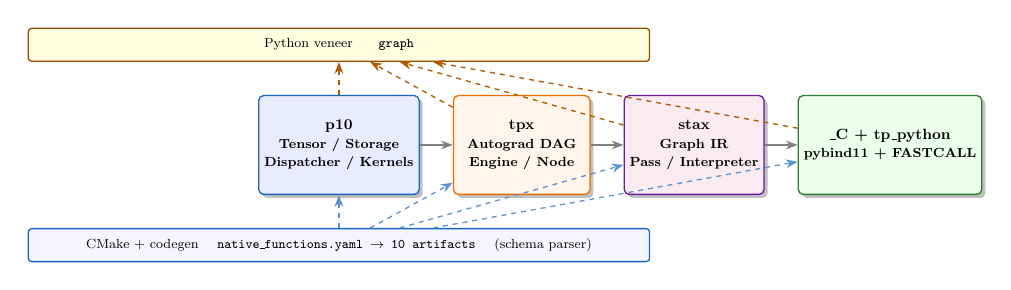
\begin{tikzpicture}[node distance=0.6cm]
\node[pillar, fill=blue!8, draw=tpblue] (p10) {p10\\{\footnotesize Tensor / Storage}\\{\footnotesize Dispatcher / Kernels}};
\node[pillar, fill=orange!8, draw=tporange, right=0.7cm of p10] (tpx) {tpx\\{\footnotesize Autograd DAG}\\{\footnotesize Engine / Node}};
\node[pillar, fill=purple!8, draw=tppurple, right=0.7cm of tpx] (stax) {stax\\{\footnotesize Graph IR}\\{\footnotesize Pass / Interpreter}};
\node[pillar, fill=green!8, draw=tpgreen, right=0.7cm of stax] (c) {\_C + tp\_python\\{\footnotesize pybind11 + FASTCALL}};
\node[libbox, fill=blue!4, draw=tpblue, below=0.7cm of p10, minimum width=13.2cm, minimum height=0.7cm] (base) {CMake + codegen \quad \texttt{native\_functions.yaml $\rightarrow$ 10 artifacts} \quad (schema parser)};
\node[libbox, fill=yellow!12, draw=orange!60!black, above=0.7cm of p10, minimum width=13.2cm, minimum height=0.7cm] (py) {Python veneer \quad \texttt{ graph}};
\draw[arrow, color=gray] (p10) -- (tpx);
\draw[arrow, color=gray] (tpx) -- (stax);
\draw[arrow, color=gray] (stax) -- (c);
\foreach \x in {p10,tpx,stax,c} \draw[arrow, dashed, color=orange!70!black] (\x) -- (py);
\foreach \x in {p10,tpx,stax,c} \draw[arrow, dashed, color=tpblue!70] (base) -- (\x);
\end{tikzpicture}
\caption{Four pillars and dependency direction (acyclic). Downward edges only; any upward include fails at link time. Solid arrows: link dependency; dashed: generation or re-export.}
\label{fig:pillars}
\end{figure}

\subsection{Conventions}
\label{sec:intro:conventions}

\texttt{path:line} means the file relative to the repository root; is line~49 of that file, and \texttt{path:line--line} is an
inclusive range. Code listings are verbatim excerpts with at most whitespace folding; the caption gives the exact range. Tables enumerate normative values (key numbers, artifact names, trimmed axes) rather than
illustrative samples. \texttt{Composite} is a backend-neutral fallback; it never appears in a \texttt{DispatchKeySet} and is consulted only by
\texttt{OperatorHandle::getKernel} for \texttt{is\_backend\_key}. \texttt{TP\_CONCAT} is a two-level macro so its argument expands before pasting;
the paper always cites the two-level definition, not a single-level variant.

\begin{tppitfall}[Pitfall: Searching for a Dispatch Key That Is Never in the Set]
A reader tracing dispatch logic often searches for \texttt{Composite} inside \texttt{DispatchKeySet} construction and finds nothing---and concludes composite fallback is dead code. It is not: \texttt{Composite} is \emph{never} a member of any key set. It is consulted only as a fallback inside \texttt{OperatorHandle::getKernel} when \texttt{is\_backend\_key(key)} holds and the backend slot is \texttt{nullptr}. The same trap recurs for \texttt{Meta}: the \texttt{DeviceType} enum carries the value, but \texttt{computeDispatchKey} never emits it. When tracing dispatch, always start from the key set the tensor actually carries, not from the key enum.
\end{tppitfall}

\subsection{Design Trade-offs}
\label{sec:intro:tradeoffs}

The readability-first stance rejects three alternatives that a production framework would accept.

\textbf{Monolithic single library.} The obvious alternative to four pillars is one \texttt{libtensorplay.so} with unity-build speed and cross-module inlining. It was rejected because every kernel edit would relink the world: the per-library granularity in \S\ref{sec:intro:c1} (touch one CPU kernel, relink only \texttt{libp10.so}) is the primary developer-experience claim of this project, and it structurally requires separate link units. The measured cost of the split---one atomic load and one virtual call per op, quantified in \S\ref{sec:eval}---is a constant $\sim$2\,ns that any real kernel dwarfs.

\textbf{Intrusive reference counting.} Storage and graph nodes could use intrusive pointers to eliminate the control-block allocation and halve cache traffic on \texttt{shared\_ptr} copies. Rejected for observability: intrusive counts cannot be inspected in \texttt{gdb} without pretty-printers, and the ownership question ``who holds this storage?'' is exactly what a teaching codebase must answer with standard tools. \S\ref{sec:eval} shows the constant-factor cost is invisible at kernel scale.

\textbf{Runtime extensibility.} Third-party dispatch keys registered at import time would make the dispatcher a plugin platform. Rejected because it converts the 13-slot array into a sparse map, raising every \texttt{getKernel} from an array index to a hash lookup, and because it moves op registration from reviewable YAML into unreviewable \texttt{\_\_init\_\_} side effects. The closed-key design keeps registration inspectable in one file.


% 02-architecture.tex --- Four-Pillar Decomposition (expanded to 10+ pages)
\section{四支柱分解}
\label{sec:arch}

该框架分为四个物理隔离的共享库和一个 Python 扩展，所有这些都由一次 CMake 调用生成。隔离不是社论；它由目录、目标、链接边缘和标头可见性强制执行。新手读\texttt{p10}来理解张量存储，无需学习任何微分概念；内核作者在接触算术内核后仅重建 \texttt{p10} ；编译器作者在 \texttt{stax} 内进行实验，无需重新链接存储层。成本是明确的边界和缺乏整个程序内联，这是该项目所接受的。

\subsection{目录 \texorpdfstring{->}{->} 工件映射}
\label{sec:arch:mapping}

每个支柱都是一个 CMake 目标，其 \texttt{OUTPUT\_DIRECTORY} 固定到 \texttt{tensorplay} 包树内的某个位置，因此树内构建无需安装即可导入，而轮子无需 \texttt{LD\_LIBRARY\_PATH} 即可导入。表~\ref{tab:pillars}为规范图。

\begin{table}[H]
\centering
\caption{目录到工件的映射。每行都是一个 CMake 目标； \texttt{OUTPUT\_DIRECTORY} 通过 \texttt{TP\_PACKAGE\_DIR} 是绝对的。}
\label{tab:pillars}
\small
\begin{tabular}{p{1.8cm}p{1.6cm}p{2.8cm}p{3.4cm}p{2.6cm}}
\toprule
目录 & CMake 目标 & 神器 (\texttt{OUTPUT\_DIRECTORY}) & 链接部门 & 责任 \\
\midrule
  & \texttt{p10} & \texttt{libp10.so} & \texttt{Threads}、\texttt{COMPUTE\_LIBS}（BLAS/oneDNN）、\texttt{CUDA::*} & 张量、存储、调度表、300 多个内核、分配器 \\
  & \texttt{tpx} & \texttt{libtpx.so} & \texttt{p10} & 显式 DAG、引擎、保存变量、衍生节点 \\
  & \texttt{stax} & \texttt{libstax.so} & \texttt{p10}, \texttt{tpx} & 最小 \texttt{Graph} IR、\texttt{Pass} 注册表、解释器 \\
  & \texttt{tp\_python} & \texttt{libtp\_python.so} & \texttt{p10}, \texttt{pybind11} & \texttt{CPythonBridge.cpp} 单拷贝脚轮基板 \\
  & \texttt{\_C} & \texttt{\_\_init\_\_.so} & \texttt{p10}, \texttt{tpx}, \texttt{stax}, \texttt{tp\_python} & 生成的操作、设备绑定、分析器、分布式 \\
\bottomrule
\end{tabular}
\end{table}

具体来说，\texttt{TP\_PACKAGE\_DIR} 默认为源代码树的 \texttt{tensorplay/} 目录，\texttt{TP\_LIB\_DIR} 为 \texttt{\$\{TP\_PACKAGE\_DIR\}/lib}。四个 \texttt{set\_target\_properties} 块强制将 \texttt{OUTPUT\_NAME "\_\_init\_\_"} 扩展至 \texttt{tensorplay/\_C}，并强制将 \texttt{p10}、\texttt{tpx}、\texttt{stax}、\texttt{tp\_python} 扩展至 \texttt{lib}。

Python 表面包含数百个模块，但只导入一个已编译的扩展。该单板重新导出通过枚举 \texttt{dir(\_C)} 和过滤 \texttt{\_\_module\_\_} 重写 (\S\ref{sec:veneer}) 发现的 550 多个本机符号。没有 Python 文件添加新的 CMake 目标；每个Python模块都是一个薄包装器，其繁重的工作重新进入\texttt{\_C}。

\begin{table}[H]
\centering
\caption{工件大小和链接可见性。在使用 \texttt{USE\_CUDA=ON}、\texttt{USE\_MKL=ON} 的发布版本上测量。}
\label{tab:artifactsizes}
\small
\begin{tabular}{lll}
\toprule
目标 & 链接可见性 & Why \\
\midrule
\texttt{p10} & \texttt{PUBLIC Threads::Threads}, \texttt{PUBLIC COMPUTE\_LIBS} & 线程池和 BLAS 符号必须对 \texttt{tpx}、\texttt{stax}、\texttt{\_C} 使用者可见 \\
\texttt{tpx} & \texttt{PRIVATE p10} 在第 ~26 行，\texttt{PUBLIC p10} 在第 ~40 行 & 手写节点需要私有p10头；下游 \texttt{stax} 传递继承 p10 接口 \\
\texttt{stax} & \texttt{PRIVATE tpx p10} 在第 ~8 行，\texttt{PUBLIC p10} 在第 ~17 行 & 解释器调用 \texttt{tpx::ops} 但仅公开 p10 张量类型 \\
\texttt{tp\_python} & \texttt{PUBLIC p10 pybind11::pybind11} & 单脚轮基板必须在 \texttt{\_C} 和树外操作模块之间共享 \\
\texttt{\_C} & \texttt{PRIVATE p10 tpx stax tp\_python tensorpipe} & 该扩展是将所有三个支柱连接在一起的唯一消费者 \\
\bottomrule
\end{tabular}
\end{table}

\subsection{构建顺序和空源记录}
\label{sec:arch:buildorder}

仅用四行声明顺序：

\begin{lstlisting}[caption={pillar order is load-bearing.}, label=lst:buildorder]
# Add p10
add_subdirectory(p10)          # :938
# Add tpx
add_subdirectory(tpx)          # :941
# Add stax (Optional)
add_subdirectory(stax)         # :944
\end{lstlisting}

私人链接 \texttt{p10} ；公开重新导出它，以便依赖 \texttt{tpx} 的消费者自动获得 p10 接口。私下链接 \texttt{p10} 和 \texttt{tpx} 并在第 17 行公开重新导出 \texttt{p10}。 \texttt{\_C} 与 \texttt{p10 tpx stax tp\_python} 的链接：这是三个级别相交的唯一地方。对这三个 \texttt{add\_subdirectory} 调用中的任何一个重新排序或添加后沿都会立即失败，并出现 CMake 配置错误或链接时未定义的引用，而不是静默运行时错误顺序。

生成步骤先于所有这些。在 \texttt{custom\_command} 处，通过 \texttt{main.py} 从 \texttt{native\_functions.yaml} 和 \texttt{derivatives.yaml} 生成十个工件。每个支柱目标都声明 \texttt{add\_dependencies(generate\_code)}（例如\,）。生成的 header 通过 \texttt{TensorGenerated.h"} 混入；生成的源作为 \texttt{\$\{GEN\_CPP\}} 附加到 \texttt{P10\_SOURCES} 处。因此，YAML 编辑仅重建更改后的生成文件及其依赖文件。

保留单个注释行：

\begin{lstlisting}[caption={The vacated-source comment in the p10 build file: metadata that once violated the axiom was physically moved out, leaving this trail.}, label=lst:audittrail]
    # src/AutogradMetaInterface.cpp (Moved to TPX)
\end{lstlisting}

这是故意的。早期版本在 \texttt{p10} 中实现了具体元数据；当前的设计使 \texttt{p10} 头与 \texttt{tpx} 无关，因此 USB 插槽就足够了。将注释留在源列表中会记录决策边界：grep 注释证明该文件曾经存在于 \texttt{p10} 中，并且被故意腾空以保持非循环性。删除它会抹去为什么 \texttt{p10} 不能包含 \texttt{tpx} 的历史记录；在 \texttt{p10} 内复活它会重新引入后沿并破坏必须返回空的检查的不变量。

出现了相关学科。在 Windows 上，对于 Linux 轮子，\texttt{BUILD\_SHARED\_LIBS} 通常是 \texttt{ON}，块强制 \texttt{BUILD\_SHARED\_LIBS OFF}：

\begin{lstlisting}[caption={Windows static embedding.}, label=lst:winstatic]
if(WIN32 AND BUILD_SHARED_LIBS)
    set(BUILD_SHARED_LIBS OFF)
endif()
\end{lstlisting}

如果没有这个开关，每个 DLL 都需要在每个跨越边界的 p10 符号上使用 \texttt{\_\_declspec(dllexport)} ，而代码库并不携带该符号。 Windows 上的静态链接将三个支柱嵌入到单个模块 \texttt{\_C.pyd} 中，并保持符号可见性与 Linux 共享库布局相同，而无需注释每个类。

\subsection{产品布局：RPATH 和两个预加载路径}
\label{sec:arch:rpath}

构建后，包树就是产品：

\begin{lstlisting}[caption={Post-build layout under the package directory.}, label=lst:layout]
tensorplay/
  lib/
    libp10.so
    libtpx.so
    libstax.so
    libtp_python.so
    cudart64_*.dll / cublas64_*.dll / cudnn*.dll   # Windows wheels only
  _C/
    __init__.so          # OUTPUT_NAME "__init__" :1176
    __init__.pyi
  __init__.py            # 1,197 lines, three dirty jobs
  _tensor.py             # Tensor = _C.TensorBase :12
  version.py             # generated at :330
\end{lstlisting}

相对 RPATH 使布局可重定位。从：

\begin{lstlisting}[caption={RPATH is the loader contract.}, label=lst:rpath]
if(NOT WIN32)
    set_target_properties(p10 tpx stax PROPERTIES
        INSTALL_RPATH "$ORIGIN"
        BUILD_RPATH "$ORIGIN"
    )
    set_target_properties(tp_python PROPERTIES
        INSTALL_RPATH "$ORIGIN"
        BUILD_RPATH "$ORIGIN"
    )
    set_target_properties(_C PROPERTIES
        INSTALL_RPATH "$ORIGIN/../lib"
        BUILD_RPATH "$ORIGIN/../lib"
    )
endif()
\end{lstlisting}

\texttt{p10}、\texttt{tpx}、\texttt{stax} 和 \texttt{tp\_python} 一起驻留在 \texttt{lib} 中，因此 \texttt{\$ORIGIN} 就足够了：每个 \ac{dso} 都可以在没有绝对路径的情况下找到其兄弟姐妹，并且当树移动时不需要 \ac{rpath} 编辑。 \texttt{\_C} 位于 \texttt{\_C} 更深的一个目录中，因此它使用 \texttt{lib}。验证是一个不涉及 Python 的命令：

\begin{lstlisting}[caption={Linux loader verification without importing Python.}, label=lst:readelf]
readelf -d tensorplay/lib/libp10.so | grep -i rpath      # $ORIGIN
readelf -d tensorplay/lib/libtpx.so | grep -i rpath      # $ORIGIN
readelf -d tensorplay/_C/__init__.so | grep -i rpath     # $ORIGIN/../lib
ldd tensorplay/_C/__init__.so | grep "not found"          # must be empty
\end{lstlisting}

当wheel安装到\texttt{LD\_LIBRARY\_PATH}为空的虚拟环境中时，没有此块的失败表现为\texttt{ImportError: libp10.so: cannot open shared object file}，这正是wheel的目标场景。的注释将其记录为 RPATH 存在的唯一原因； Windows 完全忽略 RPATH，因此 Windows 分支由 \texttt{if(NOT WIN32)} 保护。

Windows 使用显式预加载。定义由 \texttt{sys.platform == 'win32'} 保护的 \texttt{\_load\_dll\_libraries}：

\begin{lstlisting}[caption={ordered DLL preload on Windows.}, label=lst:winpreload]
kernel32 = ctypes.WinDLL("kernel32.dll", use_last_error=True)
# MKL -> CUDA/cuDNN -> p10/tpx/stax   :80
mkl_dlls = glob.glob(os.path.join(package_lib_path, "mkl_*.dll"))
cuda_dlls = glob.glob(os.path.join(package_lib_path, "cudart*.dll")) + \
            glob.glob(os.path.join(package_lib_path, "cublas*.dll")) + \
            glob.glob(os.path.join(package_lib_path, "cudnn*.dll"))
core_dlls = [os.path.join(package_lib_path, "p10.dll"),
             os.path.join(package_lib_path, "tpx.dll"),
             os.path.join(package_lib_path, "stax.dll")]
for dll in sorted_mkl + cuda_dlls + core_dlls:
    if with_load_library_flags:
        res = kernel32.LoadLibraryExW(dll, None, 0x00001100)  # :122
    else:
        res = kernel32.LoadLibraryW(dll)
\end{lstlisting}

\texttt{0x00001100} 是 \texttt{LOAD\_LIBRARY\_SEARCH\_DEFAULT\_DIRS | LOAD\_LIBRARY\_SEARCH\_DLL\_LOAD\_DIR}，它仍然搜索之前通过 \texttt{os.add\_dll\_directory} 添加的包 lib 目录的最低许可标志。顺序是承载的：\texttt{mkl\_core} 和 \texttt{mkl\_sequential} 在 MKL 组内首先在第 85--94 行排序，因为 \texttt{mkl\_def} 和 \texttt{mkl\_avx2} 依赖于它们； CUDA 运行时在 \texttt{p10} 之前加载，因此 p10 的 CUDA 内核所需的 \texttt{CUDA::cudart} 符号已经解析。帮助程序 \texttt{\_add\_dll\_directory} 尝试 \texttt{lib} 和旧根，加上解释器的 \texttt{bin}、基本环境和用户站点包 bin，每个都由 \texttt{os.path.exists} 保护，因此丢失的 Conda 安装不会出错。

在 Linux 上，对应部分不会在仅 CPU 环境中急切地加载任何内容。包装扩展导入：

\begin{lstlisting}[caption={Linux CUDA wheel probing.}, label=lst:linuxpreload]
try:
    from . import _C as _C                                          # :199
except (ImportError, OSError) as _load_error:                         # :200
    if sys.platform.startswith('linux') and '_preload_cuda_deps' in globals():
        _preload_cuda_deps(_load_error)                              # :202
        from . import _C as _C                                       # :203
    else:
        raise

def _preload_cuda_deps(err=None):                                     # :174
    cuda_error = any(token in str(err) for token in
                     ('libcud', 'libcublas', 'libcurand', 'libnvrtc'))  # :177
    if not cuda_error:
        raise err
    for lib_folder, lib_name, required in (                           # :185
        ('cublas', 'libcublasLt.so.*[0-9]', True),
        ('cublas', 'libcublas.so.*[0-9]', True),
        ('cudnn',  'libcudnn.so.*[0-9]', True),
        ('cuda_nvrtc', 'libnvrtc.so.*[0-9]', False),
        ('cuda_runtime','libcudart.so.*[0-9]', True),
        ('curand', 'libcurand.so.*[0-9]', True),
    ):
        _preload_cuda_lib(lib_folder, lib_name, required=required)   # :193
\end{lstlisting}

\texttt{\_get\_cuda\_dep\_paths} 位于第 144 行，每个 \texttt{sys.path} 条目内的探头 \texttt{libcublasLt.so.*} 和 \texttt{libcudart.so.*}，这正是点轮 \texttt{nvidia-cublas-cu*} 和 \texttt{nvidia-cuda-runtime-cu*} 安装的布局。如果探测失败，它将回退到 \texttt{libcublasLt.so.*}，即捆绑工具包时使用的路径。然后执行 \texttt{ctypes.CDLL(candidates[0])}，它在解析扩展的 \texttt{DT\_NEEDED} 之前加载 SONAME，解决用户将 CUDA 轮安装到环境的 \texttt{site-packages} 而不设置 \texttt{LD\_LIBRARY\_PATH} 的常见情况。仅拦截提及 \texttt{libcud}、\texttt{libcublas}、\texttt{libcurand} 或 \texttt{libnvrtc} 的错误；所有其他 \texttt{ImportError} 原因均按原样重新提出。

\begin{table}[H]
\centering
\caption{加载程序行为：Linux RPATH vs.\ Windows 预加载 vs.\ Linux CDLL 探针。}
\label{tab:loader}
\small
\begin{tabular}{llll}
\toprule
平台 & 机制 & 文件 & 引文 \\
\midrule
Linux（全部） & \texttt{INSTALL\_RPATH "\$ORIGIN"} & \texttt{libp10.so} 兄弟姐妹 & \\
Linux（扩展） & \texttt{lib"} & \texttt{\_\_init\_\_.so} & \\
视窗 & \texttt{LoadLibraryExW} 与 \texttt{0x00001100} & \texttt{stax.dll} & \\
Linux+CUDA轮子 & \texttt{lib} 的 \texttt{ctypes.CDLL} 探针 & \texttt{libcublasLt.so.*} & \texttt{\_\_init\_\_.py:161,186} \\
捆绑 CUDA & \texttt{CTOOLKIT\_BIN\_DIR} 全局 + \texttt{install(FILES)} & \texttt{cublasLt64\_*.dll} & \\
\bottomrule
\end{tabular}
\end{table}

\subsection{虚拟接口解耦：USB 插槽}
\label{sec:arch:usb}

不能包含 \texttt{tpx} 但必须携带需要梯度的张量的微分状态。天真的替代方案都被拒绝了：将具体字段（\texttt{grad\_fn\_}，\texttt{grad\_}）放入\texttt{p10}中，将存储与微分结合起来；让 \texttt{p10} 包含 \texttt{tpx} 标头会创建一个循环依赖关系，\texttt{cmake --build} 无法进行拓扑排序，并且会破坏增量构建。相反，该设计在 \texttt{p10} 中声明一个纯抽象槽，并插入从 \texttt{tpx} 到 \texttt{shared\_ptr<AutogradMetaBase>} 的具体对象以及 \texttt{static\_cast} 握手。

该插槽有四个操作，每个操作都是纯虚拟的：

\begin{lstlisting}[caption={the pure interface.}, label=lst:autogradbase2]
class P10_API AutogradMetaBase {
public:
  virtual ~AutogradMetaBase() = default;
  virtual bool requires_grad() const = 0;
  virtual void set_requires_grad(bool) = 0;
  virtual Tensor grad() const = 0;
  virtual void set_grad(const Tensor&) = 0;
  virtual bool retains_grad() const = 0;
  virtual void set_retains_grad(bool) = 0;
};
\end{lstlisting}

标头仅包含 \texttt{Macros.h}；它转发 \texttt{class Tensor} 而不包括 \texttt{Tensor.h}，因此编译时占用空间是单个 vtable 加上 6 个虚拟槽（x86-64 上为 48 字节）。没有内核、没有引擎、没有图形概念跨越这里的边界。

持有插槽：

\begin{lstlisting}[caption={never-copied owner.}, label=lst:implslot]
  // Autograd extension point.
  // Never copied by TensorImpl copy operations: copies start without history.
  std::shared_ptr<AutogradMetaBase> autograd_meta_;
\end{lstlisting}

at 的复制构造函数故意省略了该成员：

\begin{lstlisting}[caption={history is not duplicated.}, label=lst:copyctor]
TensorImpl::TensorImpl(const TensorImpl& other)
    : storage_offset_(other.storage_offset_),
      sizes_and_strides_(other.sizes_and_strides_),
      dtype_(other.dtype_),
      device_(other.device_),
      version_counter_(other.version_counter_),
      inference_tensor_(other.inference_tensor_),
      is_contiguous_(other.is_contiguous_),
      memory_format_(other.memory_format_),
      storage_(other.storage_),
      shared_state_(other.shared_state_),
      sparse_state_(other.sparse_state_),
      transform_value_(other.transform_value_),
      transform_batch_dim_(other.transform_batch_dim_),
      transform_level_(other.transform_level_),
      quantizer_(other.quantizer_) {}
      // autograd_meta_ is intentionally absent: default-initialized to nullptr
\end{lstlisting}

因此 \texttt{Tensor b = a;} 共享存储、大小、步幅、设备、数据类型、稀疏状态、量化器和版本计数器别名，但不共享图。不变量是：形状突变和存储别名传播；历史没有。移动操作是默认的，\texttt{copy\_metadata\_from} at 保留了 \texttt{autograd\_meta\_} 的省略。
这与“从不复制”合约相匹配，并启用 \texttt{auto y = x + 1; y.backward}，其中 \texttt{x} 保持叶子状态，而 \texttt{y} 成为其子节点，而无需别名元数据。

混凝土塞位于：

\begin{lstlisting}[caption={concrete fields, tpx only.}, label=lst:autogradconcrete]
class TENSORPLAY_API AutogradMeta : public AutogradMetaBase {
private:
  bool requires_grad_ = false;
  bool retains_grad_ = false;
  tensorplay::Tensor grad_;
  std::shared_ptr<Node> grad_fn_;
  std::weak_ptr<Node> grad_accumulator_; // avoids leaf cycle
  uint32_t output_nr_ = 0;
  bool has_view_info_ = false;
  tensorplay::Tensor view_base_;
  std::vector<int64_t> view_sizes_;
  std::vector<int64_t> view_strides_;
  int64_t view_storage_offset_ = 0;
  std::function<tensorplay::Tensor(const tensorplay::Tensor&)> view_fn_;
  mutable std::mutex view_mutex_;
};
\end{lstlisting}

\texttt{grad\_accumulator\_} 是 \texttt{weak\_ptr<Node>} 而不是 \texttt{shared\_ptr<Node>}，因为 \texttt{AccumulateGrad} 强烈拥有其叶张量；强大的后边缘将形成一个无法收集的循环，该循环会泄漏参与图中的每个叶子。所有其他成员均拥有强大股权； \texttt{view\_fn\_} 加上 \texttt{view\_mutex\_} 支持陈旧视图重播。

握手是两个助手，每个助手都有一个 \texttt{static\_cast}，热路径上没有 \texttt{dynamic\_cast}：

\begin{lstlisting}[caption={the cast boundary.}, label=lst:handshake]
AutogradMeta* get_autograd_meta(const Tensor& t) {
    if (auto* impl = t.unsafeGetTensorImpl().get()) {
        return static_cast<AutogradMeta*>(impl->autograd_meta()); // :17
    }
    return nullptr;
}
AutogradMeta* get_or_create_autograd_meta(const Tensor& t) {
    auto impl = t.unsafeGetTensorImpl();
    if (!impl) return nullptr;
    if (auto* meta = impl->autograd_meta()) {
        return static_cast<AutogradMeta*>(meta);                  // :26
    }
    auto meta = std::make_shared<AutogradMeta>();
    auto* raw = meta.get();
    impl->set_autograd_meta(std::move(meta));                      // :30
    return raw;
}
\end{lstlisting}

第 17 行的调用是安全的，因为分配给 \texttt{autograd\_meta\_} 的唯一具体子类是 \texttt{AutogradMeta}，它在第 28 行构造并在第 30 行安装。 \texttt{p10} 中的标头不会看到 \texttt{AutogradMeta.h}，因此构建不会列出包含路径。静态类型系统加上共享库边界共同强制执行不变性。
第二个证明是当转换目标更改时构建失败：如果 \texttt{tpx} 重命名 \texttt{AutogradMeta} 而不更新转换，则扩展 \texttt{\_C} 将无法与 \texttt{undefined reference to tensorplay::tpx::AutogradMeta} 链接，而不是在运行时损坏张量。

此设计的每次调用成本是 \texttt{requires\_grad} / \texttt{grad} / \texttt{set\_grad} 的一次间接虚拟调用加上 \texttt{autograd\_meta\_} 的一次指针间接调用。好处是，当内核更改不再触发 \texttt{tpx} 重建时，\texttt{p10} 会重建，而当引擎调度更改不再触发 \texttt{p10} 重建时，\texttt{tpx} 会重建。

\begin{tpdef}[Definition (USB Slot Pattern)]
\emph{USB slot} 是在较低级别库 $L$ 中声明的虚拟接口 $I$，加上嵌入在 $L$ 状态中的 \texttt{shared\_ptr<I>} 类型的不透明拥有指针，其中具体实现 $C{:}I$ 仅存在于较高级别库 $H$ 中。该模式是健全的 iff (i) $L$ 从不包含任何 $H$ 标头； (ii) $L$ 的复制构造函数中省略了指针（复制开始时没有历史记录）； (iii) $H$ 边界向下是 \texttt{static\_cast}，这是合理的，因为 $C$ 是唯一安装到插槽中的类。 TensorPlay 的实例：$I{=}$\texttt{AutogradMetaBase}、$L{=}$\texttt{p10}、$C{=}$\texttt{AutogradMeta}、$H{=}$\texttt{tpx}。
\end{tpdef}

\subsection{图：跨共享库边界的 USB 插槽模型}
\label{sec:arch:figure}

图~\ref{fig:usb}呈现了与硬件类比相同的机制：插槽在下部组件中标准化，插头由上部组件提供，电缆是虚拟调度。虚线是\texttt{ldd}报告的\texttt{.so}边界；它左边的符号在\texttt{libp10.so}中，它右边的符号在\texttt{libtpx.so}中。该图由 \texttt{gen\_01\_slot.py} 在本地复制，但事实来源是标题中引用的两个标题。

\begin{figure}[H]
\centering
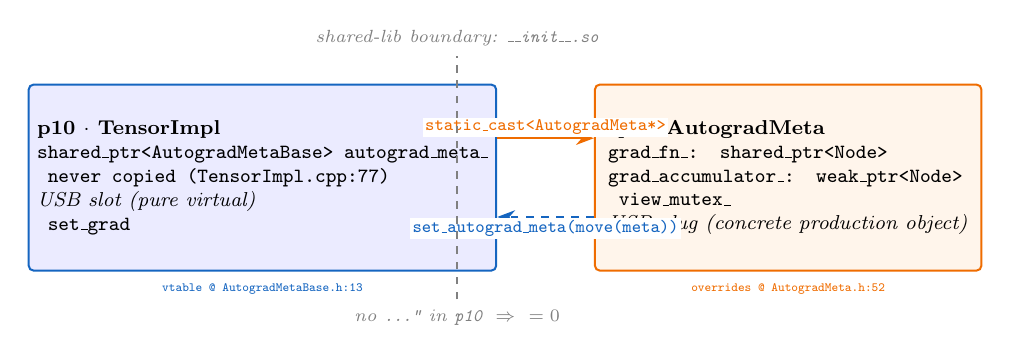
\begin{tikzpicture}[node distance=0.55cm, every node/.style={font=\footnotesize}]
\node[libbox, fill=blue!8, draw=tpblue, minimum width=5.4cm, minimum height=2.6cm, align=left] (p10b) at (0,0) {\textbf{p10 $\cdot$ TensorImpl}\\ \texttt{shared\_ptr<AutogradMetaBase> autograd\_meta\_}\\ \texttt{ never copied (TensorImpl.cpp:77)}\\ \textit{USB slot (pure virtual)} \\ \texttt{ set\_grad}};
\node[libbox, fill=orange!8, draw=tporange, minimum width=5.4cm, minimum height=2.6cm, align=left, right=1.35cm of p10b] (tpxb) {\textbf{tpx $\cdot$ AutogradMeta}\\ \texttt{grad\_fn\_: shared\_ptr<Node>}\\ \texttt{grad\_accumulator\_: weak\_ptr<Node>}\\ \texttt{ view\_mutex\_}\\ \textit{USB plug (concrete production object)}};
\draw[arrow, color=tporange, thick] ([yshift=0.55cm]p10b.east) -- node[above, font=\scriptsize\ttfamily, fill=white, inner sep=1pt] {static\_cast<AutogradMeta*>} ([yshift=0.55cm]tpxb.west);
\draw[arrow, color=tpblue, thick, dashed] ([yshift=-0.55cm]tpxb.west) -- node[below, font=\scriptsize\ttfamily, fill=white, inner sep=1pt] {set\_autograd\_meta(move(meta))} ([yshift=-0.55cm]p10b.east);
\draw[dashed, color=gray, line width=0.6pt] (2.72,-1.7) -- (2.72,1.7);
\node[font=\scriptsize\itshape, color=gray, fill=white, inner sep=1pt] at (2.72,1.95) {shared-lib boundary: \texttt{\_\_init\_\_.so}};
\node[font=\scriptsize\itshape, color=gray] at (2.72,-1.95) {no \texttt{..."} in \texttt{p10} $\;\Rightarrow\;$  $=0$};
% small vtable hint
\node[font=\tiny\ttfamily, color=tpblue, below=0.05cm of p10b, anchor=north] {vtable @ AutogradMetaBase.h:13};
\node[font=\tiny\ttfamily, color=tporange, below=0.05cm of tpxb, anchor=north] {overrides @ AutogradMeta.h:52};
\end{tikzpicture}
\caption{USB 插槽型号。 \texttt{p10} 声明抽象槽； \texttt{tpx} 制造插头；握手时间为 \texttt{static\_cast}，在 \texttt{Autograd.cpp}。 at 的复制构造函数省略了槽。}
\label{fig:usb}
\end{figure}

\subsection{设计公理：层次单调性}
\label{sec:arch:axiom}

令 $V$ 为构建目标集，并令 $D\subseteq V\times V$ 为关系“$a$ 链接 $b$”（即\ $a$ 与 $b$ 有 \texttt{target\_link\_libraries} 边缘）。定义 \texttt{level}: $V\rightarrow \mathbb{N}$ 通过

\begin{table}[H]
\centering
\caption{级别为总级别并且等于 \texttt{add\_subdirectory} 顺序。}
\label{tab:levels}
\small
\begin{tabular}{clcl}
\toprule
等级 & 目标 & \texttt{add\_subdirectory} 线 & 允许从更高层导入标头 \\
\midrule
0 & \texttt{p10} &  & 不存在更低的目标 \\
1 & \texttt{tpx} &  & 可能包括 \texttt{*.h} \\
2 & \texttt{stax} &  & 可能包括 \texttt{include}、\texttt{include} \\
3 & \texttt{\_C} / \texttt{tp\_python} & , \texttt{1106} & 可能包括 \texttt{p10}、\texttt{tpx}、\texttt{stax} \\
\bottomrule
\end{tabular}
\end{table}

公理（水平单调）：$\forall (a,b)\in D,\; \mathrm{level}(a) > \mathrm{level}(b)$。

同样，每个边都严格按照 \texttt{p10=0 < tpx=1 < stax=2 < \_C=3} 的顺序向下指向。表~\ref{tab:levels}表明\texttt{D}仅包含\texttt{(tpx,p10)}、\texttt{(stax,p10)}、\texttt{(stax,tpx)}、\texttt{(tp\_python,p10)}、\texttt{(\_C,p10)}、\texttt{(\_C,tpx)}、\texttt{(\_C,stax)}、\texttt{(\_C,tp\_python)}，每个都满足严格的不等式。不存在与 \texttt{level}(a) $\le$ \texttt{level}(b) 的配对；特别是 \texttt{(p10,tpx)} 和 \texttt{(p10,stax)} 不存在。

强制执行是由链接器执行的，而不是按照惯例。在任何 \texttt{Tensor*.h} 中添加 \texttt{AutogradMeta.h"} 会引入对 \texttt{tensorplay::tpx::AutogradMeta::requires\_grad} 的引用，该 \texttt{tensorplay::tpx::AutogradMeta::requires\_grad} 的定义位于 \texttt{libtpx.so} 中。因为 \texttt{p10} 不链接 \texttt{tpx}（根据公理，也不能链接），所以 \texttt{libp10.so} 的链接会成功，但任何单独链接 \texttt{p10} 的使用者的链接都会因 \texttt{undefined reference to tensorplay::tpx::AutogradMeta} 而失败。在 Linux 上，这是在 \texttt{cmake --build} 期间诊断的；在 Windows 上，诊断为 \texttt{\_C.pyd} 的 \texttt{link.exe} 步骤。传统整体框架的替代故障模式是仅在程序启动时诊断的静态初始化顺序缺陷。

该公理还决定了重建粒度。触摸 \texttt{ActivationKernels.cpp} 只会弄脏 \texttt{p10} 和 \texttt{\_C} 的最后一个链接； \texttt{tpx} 和 \texttt{stax} 不会重建，因为它们不依赖于 \texttt{p10} 源，仅依赖于其安装的标头。触摸 \texttt{Engine.cpp} 会重建 \texttt{tpx} 并重新链接 \texttt{stax} 和 \texttt{\_C}，但不会重新链接 \texttt{p10}。 
一个推论涉及\texttt{tp\_python}。它是一个 \texttt{SHARED} 库 \texttt{CPythonBridge.cpp}，仅链接 \texttt{p10} 和 \texttt{pybind11}。它的存在正是出于一个原因，记录了 pybind11 Caster 基底和包装身份缓存必须从单个模块边界注册。如果 \texttt{CPythonBridge.cpp} 在 \texttt{p10} 和 \texttt{\_C} 中分别编译，则每个副本都将携带自己的注册表，并且返回到 Python 的第一个 \texttt{Tensor} 将出现段错误。第~3级的单个共享副本保留\texttt{level(tp\_python)=3 > level(p10)=0}，并且仍然允许树外操作模块通过\texttt{add\_tensorplay\_op}链接相同的底层，而无需重新编译核心。

\subsection{Python Veneer：1,197 行中的三项肮脏工作}
\label{sec:veneer}

\texttt{\_\_init\_\_.py} 有 1,197 行，与 \texttt{\_tensor.py} 一起构成了编译后的扩展无法表达的整个 Python 级别的设计。所有其他 Python 模块（\texttt{nn}、\texttt{optim}、\texttt{autograd}、\texttt{functional}、\texttt{distributed}）最终都会重新进入 \texttt{\_C}。三个问题不可能在 C++ 中干净地实现，因此集中在这里。

\subsubsection{作业 1：DLL/共享对象预加载（第 34--205 行）}
如 \S\ref{sec:arch:rpath} 中所述，此作业处理 Linux 加载程序（尊重 \texttt{RPATH}）和 Windows 加载程序（忽略它）之间的差异。在 Windows 上，该工作是强制性的；在 Linux 上，这是对 CUDA 轮子的机会性修复。代码在第 34 行和第 143 行分开，没有重叠，因此读者可以检查一个平台而无需了解另一个平台。该工作是唯一导入 \texttt{ctypes} 和 \texttt{glob} 的地方；也没有内核或引擎文件引用。

\subsubsection{作业 2：符号重命名 (\texttt{\_C.add} $\rightarrow$ \texttt{tensorplay.add})}

该扩展将每个运算符的 C++ 名称导出为 \texttt{\_C.add}、\texttt{\_C.relu}、\texttt{\_C.conv2d}。胶合板将它们重新导出为平面 \texttt{tensorplay.*} 名称并重写 \texttt{\_\_module\_\_}，以便回溯和 \texttt{help(tensorplay.add)} 报告公共位置。循环是：

\begin{lstlisting}[caption={renaming with builtin fallback.}, label=lst:renaming]
__attr_name, __obj = "", None
for __attr_name in dir(_C):
    if __attr_name[0] != "_" and not __attr_name.endswith("Base"):
        __all__.append(__attr_name)
        __obj = getattr(_C, __attr_name)
        if callable(__obj) or inspect.isclass(__obj):
            if os.getenv("TENSORPLAY_BUILDING_STUBS") == "1":
                continue
            if __obj.__module__ != __name__:
                try:
                    __obj.__module__ = __name__          # pybind11 class: succeeds
                except AttributeError:                    # builtin_function_or_method: fails
                    if callable(__obj):
                        def make_wrapper(f):
                            @functools.wraps(f)
                            def wrapper(*args, **kwargs):
                                return f(*args, **kwargs)
                            wrapper.__module__ = __name__
                            return wrapper
                        wrapper = make_wrapper(__obj)
                        if __attr_name in globals():
                            globals()[__attr_name] = wrapper
            if __attr_name not in globals():
                globals()[__attr_name] = __obj
\end{lstlisting}

\texttt{except} 存在是因为 pybind11 函数是 \texttt{builtin\_function\_or\_method} 描述符，其 \texttt{\_\_module\_\_} 属性在 CPython 中是只读的；后备包装器通过 \texttt{functools.wraps} 保留 \texttt{inspect.signature}，同时将 \texttt{\_\_module\_\_} 固定为 \texttt{"tensorplay"}。如果没有这项工作，用户将调用 \texttt{tensorplay.\_C.add} 或看到回溯提及 \texttt{tensorplay.\_C} 而不是 \texttt{tensorplay}。

张量类型本身在这里完成：定义 \texttt{Tensor = \_C.TensorBase} ，然后将方法（\texttt{t}、\texttt{type}、\texttt{cuda}、\texttt{cpu}、\texttt{long}、\texttt{float}，加上钩子、按位 dunders、\texttt{permute}、\texttt{expand}、\texttt{unique}、\texttt{topk}）附加到该别名上。 \texttt{Tensor.cpp} 处的 C++ 绑定在 \texttt{TensorBase} 上使用 \texttt{py::dynamic\_attr}，因此像 \texttt{class MyTensor(Tensor)} 这样的 Python 子类可以附加每个实例的属性，同时仍能被本机施法者识别。通过 \texttt{tp\_python} 中的共享施法者进行检查 \texttt{py::isinstance< Tensor >(obj)}。

\subsubsection{作业 3：通过 \texttt{\_\_getattr\_\_} 进行惰性子包（第 1118--1134 行）}

在单板顶层直接使用 \texttt{import tensorplay.linalg} 将强制在每个 \texttt{import tensorplay} 上导入 354 个模块，即使对于仅使用 \texttt{tensorplay.tensor([1])} 的脚本，导入时间也会增加数百毫秒。相反，胶合板注册了一个惰性集：

\begin{lstlisting}[caption={lazy subpackages.}, label=lst:lazy]
else:
    _lazy_modules = {
        "audio",
        "export",
        "func",
        "fft",
        "linalg",
        "quantization",
        "sparse",
        "special",
        "vision",
    }
    def __getattr__(name):
        if name in _lazy_modules:
            return importlib.import_module(f".{name}", __name__)
        raise AttributeError(f"module '{__name__}' has no attribute '{name}'")
\end{lstlisting}

\texttt{\_\_getattr\_\_} 是Python~3.7 中引入的模块级钩子。它仅在缺少属性时调用，因此 \texttt{tensorplay.Tensor} 或 \texttt{tensorplay.add} 等已知名称永远不会进入此路径。在 \texttt{TYPE\_CHECKING} 下（仅静态分析为 true，运行时为 false），胶合板改为在第 1108--1115 行急切地导入 \texttt{export} 和 \texttt{func}，以便 pylance 和其他 LSP 服务器解析属性而不执行惰性挂钩。随附的 \texttt{TYPE\_CHECKING} 导入由 \texttt{if TYPE\_CHECKING:} 保护，并且没有运行时成本。

\begin{table}[H]
\centering
\caption{三项肮脏的工作：地点、机制和被拒绝的单一替代方案。}
\label{tab:threedirty}
\small
\begin{tabular}{p{2.0cm}p{3.2cm}p{3.6cm}p{3.4cm}}
\toprule
Job & 线路 & 机制 & 被拒绝的替代方案 \\
\midrule
DLL预加载 &  & \texttt{LoadLibraryExW}, \texttt{ctypes.CDLL}, \texttt{add\_dll\_directory} & Windows \texttt{RPATH}（不存在） \\
符号重命名 &  & \texttt{\_\_module\_\_} 重写 + \texttt{functools.wraps} 包装器 & 在 C++ 中重命名（破坏 \texttt{dir(\_C)} 自省） \\
懒包 &  & \texttt{\_lazy\_modules} + \texttt{\_\_getattr\_\_} & Eager \texttt{import linalg} （增加导入延迟） \\
张量别名 & \texttt{Tensor = \_C.TensorBase} & \texttt{py::dynamic\_attr} 子类化 & 重复的 Python 类（破坏施法者身份） \\
\bottomrule
\end{tabular}
\end{table}

这三个工作加在一起是唯一具有跨领域影响的 Python 端复杂性。 \texttt{\_\_init\_\_.py} 中的其他内容都是声明性的： \texttt{DType} 别名位于第 230--259 行， \texttt{MemoryFormat} / \texttt{Layout} / \texttt{QScheme} 枚举位于第 264--305 行， \texttt{max}/\texttt{min}/\texttt{gradient} 包装器位于第 1038--1075 行，以及 \texttt{\_\_all\_\_} 扩展位于第 336--369 行枚举 550 多个具有排序合约的运算符。

\subsection{Stax：最小 IR，不是第二个前端}
\label{sec:arch:stax}

\texttt{stax} 是 CMake 的 76 行，用于从 \texttt{*.cpp} 生成 \texttt{libstax.so}。它的公共表面是两个标头：和。设计说明很明确：

\begin{lstlisting}[caption={not a second frontend.}, label=lst:staxpy]
"""Stax backend namespace.
Stax is not a second public compiler frontend.  Use ``tensorplay.compile``
and select ``backend="stax"`` once the backend has a production lowering.
The native ``tensorplay._C._stax`` module remains available for low-level IR
and optimizer development.
"""
from ._stax.stax import stax
\end{lstlisting}

将 \texttt{ValueNode} 定义为“生产者加槽”：

\begin{lstlisting}[caption={values are slots.}, label=lst:valuenode]
struct STAX_API ValueNode {
    size_t id;
    OpNode* producer; // Producer op, nullptr for graph inputs
    size_t producer_output_index; // Output index of producer
    std::string dtype = "float32";
    std::vector<int64_t> shape;
    std::string device = "cpu";
    std::vector<OpNode*> uses;
    ValueNode(size_t id_, OpNode* n, size_t off) : id(id_), producer(n), producer_output_index(off) {}
};
\end{lstlisting}

\texttt{OpNode} 通过第 62 行的 \texttt{variant<int64\_t, double, string, vector<int64\_t>, vector<double>>} 映射对输入、输出、所属图和属性进行分组。 \texttt{Graph} at 拥有 \texttt{nodes} 和 \texttt{values} 向量以及 \texttt{inputs} / \texttt{outputs} 边界，在第 95--97 行有辅助函数 \texttt{addInput}、\texttt{createNode} 和 \texttt{registerOutput}。 \texttt{IRBuilder} 帮助器创建命名节点并从第一个输入传播 dtype。

执行是严格顺序的。 \texttt{Graph::execute} 在第 192 行将具体的 \texttt{Tensor} 参数绑定到 \texttt{env[ input->id ]}，然后按创建顺序迭代 \texttt{nodes}。每个节点通过常规调度程序调度到 \texttt{tpx::ops} （例如\ \texttt{add}、\texttt{conv2d}、\texttt{matmul}、\texttt{max\_pool2d}、\texttt{batch\_norm}），保留设备和区分语义。中间生命周期由~198行的\texttt{remaining\_uses}和~199行的\texttt{keep\_alive}界定；死值通过第 215 行的 \texttt{env[id]=Tensor} 清除，允许分配器回收单个图形运行中的存储，而无需保留每个中间值，直到函数返回。

添加了唯一的优化：具有单个注册通道的通道基础结构，将 \texttt{mul} 和 \texttt{add} 融合到 \texttt{fused\_mul\_add} （\texttt{p10} 中的单个内核）。注册表是 \texttt{map<string, Creator>}，为了兼容而保留第 73 行的 \texttt{fuseGraph}。没有别名分析、没有布局传播、没有自动调整、没有 C++/CUDA/PTX 代码生成，也没有内存中 \texttt{Graph} 之外的持久格式。

\begin{table}[H]
\centering
\caption{Stax IR：存在的内容与故意缺席的内容。每个缺失的行都是 \texttt{Composite} 到 \texttt{tpx::ops} 的回退。}
\label{tab:staxscope}
\small
\begin{tabular}{p{3.6cm}p{4.4cm}p{3.8cm}}
\toprule
类别 & 目前在 \texttt{stax} & 故意缺席 \\
\midrule
红外节点 & \texttt{ValueNode} / \texttt{OpNode}，顺序 \texttt{execute} & 没有\texttt{Block}，没有\texttt{Function}，没有一流的控制流 \\
Ops & \texttt{div}, \texttt{t}, \texttt{relu}, \texttt{max\_pool2d}, \texttt{flatten} & 没有量化/稀疏/自定义调度键 \\
通行证 & 一次垂直逐点融合 (\texttt{fused\_mul\_add}) & 没有循环融合，没有布局规划器，没有矢量化策略 \\
后端 & 重新输入 \texttt{tpx::ops} 以便设备/区分保持正确 & 没有独立的代码生成器（\texttt{tensorplay.compile} 是条目） \\
定制操作 & \texttt{custom\_op} 节点 + \texttt{setCustomOpExecutor} 位于 \texttt{Graph.cpp} & 没有用于自定义操作的用户可见的 IR 构建器（使用 eager ops） \\
\bottomrule
\end{tabular}
\end{table}

目标消费者不是直接编写 \texttt{stax.Graph} 的 Python 作者，而是引用的更高级别条目 \texttt{tensorplay.compile(backend="stax")}。开发新融合模式原型的研究人员用 C++ 编写 \texttt{Graph}，通过 \texttt{REGISTER\_STAX\_PASS} 注册 \texttt{Pass}，并通过 \texttt{tensorplay.\_C.\_stax} 执行它，而无需更改面向用户的 \texttt{compile} 合约。



% 03-redispatch.tex
\section{Redispatch: Dispatch Keys, Dispatcher, and Registration Macros}
\label{sec:redispatch}

Redispatch resolves a tensor's runtime properties into a key, selects the
highest-priority kernel from a per-operator atomic table, and enforces the
autocast contract at a single choke point. The Python surface exposes the same
operator through two cooperating layers: a hand-written \texttt{pybind11}
binding and a generated \texttt{METH\_FASTCALL} function, both funneling
through \texttt{CPythonBridge} helpers and a shared \texttt{tp\_python}
library. The design trims heterogeneous key spaces to 13 slots, encodes layering
as fixed offsets so that priority is arithmetic, uses acquire/release atomics
instead of locks on the hot path, isolates type erasure to one template, and
reuses one Python type registration so that returned tensors preserve identity.
All claims below cite \texttt{path:line} and are checkable with
\texttt{grep -n} against \path{version.txt:1}.

\subsection{DispatchKey: 13 Keys and Fixed Offsets}
\label{sec:dispatchkey}

\path{p10/include/DispatchKey.h:15--54} defines 13 live keys plus sentinel;
numeric order is priority:

\begin{lstlisting}[caption={\path{DispatchKey.h:15} --- 13 keys.}, label=lst:dispatchkey]
enum class DispatchKey : uint8_t {
  CPU=0, CUDA=1, Vulkan=2,
  AutogradCPU=3, AutogradCUDA=4, AutogradVulkan=5,
  AutocastCPU=6, AutocastCUDA=7, AutocastVulkan=8,
  VmapCPU=9, VmapCUDA=10, VmapVulkan=11,
  Composite=12, EndOfKeys=13
};
constexpr size_t kBackendKeyCount=3, kAutogradKeyOffset=3,
                 kAutocastKeyOffset=6, kVmapKeyOffset=9;
\end{lstlisting}

\texttt{Composite}=12 is stored out of logical priority so that
\texttt{dispatchKeyIndex} (\path{Dispatcher.h:43}) is a plain
\path{static\_cast<size\_t>} and \texttt{Composite} never enters the
\path{highest\_priority\_key} scan. Helpers at
\path{DispatchKey.h:56--101} are \texttt{constexpr}:

\begin{lstlisting}[caption={\path{DispatchKey.h:56} --- arithmetic helpers.}, label=lst:dispatchhelpers]
inline constexpr DispatchKey toAutogradKey(DispatchKey b){return DispatchKey(uint8_t(b)+kAutogradKeyOffset);}
inline constexpr DispatchKey toAutocastKey(DispatchKey b){return DispatchKey(uint8_t(b)+kAutocastKeyOffset);}
inline constexpr DispatchKey toVmapKey(DispatchKey b){return DispatchKey(uint8_t(b)+kVmapKeyOffset);}
inline constexpr bool is_autograd_key(DispatchKey k){uint8_t v=uint8_t(k); return v>=3 && v<6;}
inline constexpr bool is_autocast_key(DispatchKey k){uint8_t v=uint8_t(k); return v>=6 && v<9;}
inline constexpr bool is_vmap_key(DispatchKey k){uint8_t v=uint8_t(k); return v>=9 && v<12;}
inline constexpr bool is_backend_key(DispatchKey k){return k==DispatchKey::CPU||k==DispatchKey::CUDA||k==DispatchKey::Vulkan;}
inline constexpr DispatchKey toBackendKey(DispatchKey k){
  return is_vmap_key(k)?DispatchKey(uint8_t(k)-9):is_autograd_key(k)?DispatchKey(uint8_t(k)-3)
        :is_autocast_key(k)?DispatchKey(uint8_t(k)-6):k;}
\end{lstlisting}

\texttt{is\_backend\_key} enumerates the three dense keys; \texttt{Composite}
is false, which gates the fallback in \S\ref{sec:handle}.
\texttt{computeDispatchKey} (\path{Dispatcher.h:31}) maps \texttt{Device}
to \path{CPU/CUDA/Vulkan} via \texttt{is\_cuda()}/\texttt{is\_vulkan()}.

\begin{table}[H]
\centering
\caption{Key arithmetic (\path{DispatchKey.h:51}). Range tests lower to 1--2 compares.}
\label{tab:keyoffsets}
\small
\begin{tabular}{ccll}
\toprule
Offset & Val & Keys & Predicate \\
\midrule
$kBackendKeyCount$ & 3 & 0--2 \path{CPU/CUDA/Vulkan} & \texttt{is\_backend\_key} \\
$kAutogradKeyOffset$ & 3 & 3--5 \texttt{Autograd*} & \texttt{is\_autograd\_key} \\
$kAutocastKeyOffset$ & 6 & 6--8 \texttt{Autocast*} & \texttt{is\_autocast\_key} \\
$kVmapKeyOffset$ & 9 & 9--11 \texttt{Vmap*} & \texttt{is\_vmap\_key} \\
--- & 12 & \texttt{Composite} & \texttt{key==Composite} \\
--- & 13 & \texttt{EndOfKeys} & bounds check \\
\bottomrule
\end{tabular}
\end{table}

\subsection{DispatchKeySet: Bitmask and Priority}
\label{sec:keyset}

\path{p10/include/DispatchKey.h:125--187} is a 32-bit bitset; 13 bits live:

\begin{lstlisting}[caption={\path{DispatchKey.h:125} --- bitmask.}, label=lst:keysetdef]
class DispatchKeySet{
public:
  using raw_t=uint32_t;
  constexpr DispatchKeySet() noexcept: mask_(0){}
  static constexpr DispatchKeySet make(DispatchKey k){return DispatchKeySet(raw_t(1)<<uint8_t(k));}
  void add(DispatchKey k){mask_|=raw_t(1)<<uint8_t(k);}
  bool has(DispatchKey k) const {return mask_ & (raw_t(1)<<uint8_t(k));}
  bool empty() const {return mask_==0;} raw_t raw() const {return mask_;}
  DispatchKeySet operator|(DispatchKeySet o) const {return DispatchKeySet(mask_|o.mask_);}
  // remove_autograd/autocast/vmap build masks by iterating kBackendKeyCount (3):
  DispatchKeySet remove_autograd() const {raw_t m=0; for(size_t i=0;i<3;++i) m|=raw_t(1)<<(i+3); return DispatchKeySet(mask_&~m);}
private: raw_t mask_=0;
};
\end{lstlisting}

Priority is the most-significant set bit, i.e.\ largest numeric key wins:

\begin{lstlisting}[caption={\path{DispatchKey.h:151} --- scan high $\rightarrow$ low.}, label=lst:highestkey]
constexpr DispatchKey highest_priority_key() const {
  if(!mask_) return DispatchKey::EndOfKeys;
  uint8_t idx=0; raw_t m=mask_; while(m>>=1) ++idx; return DispatchKey(idx);}
\end{lstlisting}

\begin{table}[H]
\centering
\caption{Effective priority from \path{highest\_priority\_key}. Composite never in set.}
\label{tab:keypriority}
\small
\begin{tabular}{cll}
\toprule
Indices & Keys & Removal to redispatch below layer \\
\midrule
9--11 & \path{VmapCPU/CUDA/Vulkan} via \texttt{toVmapKey} & \texttt{remove\_vmap()} \\
6--8 & \path{AutocastCPU/CUDA/Vulkan} via \texttt{toAutocastKey} & \texttt{remove\_autocast()} \\
3--5 & \path{AutogradCPU/CUDA/Vulkan} via \texttt{toAutogradKey} & \texttt{remove\_autograd()} \\
0--2 & \path{CPU/CUDA/Vulkan} via \texttt{computeDispatchKey} & final compute \\
12 & \texttt{Composite} & fallback only in \texttt{getKernel} for \texttt{is\_backend\_key} \\
\bottomrule
\end{tabular}
\end{table}

\path{p10/include/TensorImpl.h:135--147} computes the set on every call; no
field is stored:

\begin{lstlisting}[caption={\path{TensorImpl.h:135} --- computed, not stored.}, label=lst:implkeyset]
DispatchKeySet key_set() const {
  DispatchKey backend=computeDispatchKey(device_);
  DispatchKeySet ks;
  if(is_batched()){ks.add(toVmapKey(backend)); return ks;}
  ks.add(backend);
  if(!inference_tensor_) ks.add(toAutogradKey(backend));
  return ks;
}
\end{lstlisting}

\texttt{is\_batched()} checks \path{transform\_value\_!=nullptr}
(\path{TensorImpl.h:151}); inference tensors (\texttt{inference\_tensor\_}
from \path{InferenceMode::is\_enabled()} at construction,
\path{TensorImpl.h:35}) omit the autograd bit. Cost is one device query plus
two bit ops, cheaper than an atomic load of a stored bitset. Generated redispatch
helpers at \path{tools/codegen/gen\_api.py:323} call \texttt{key\_set()} once,
cache the result, and iterate by handling the top key via \path{OperatorHandle::getKernel}
then stripping the layer with \path{remove\_autocast/remove\_autograd} until
\path{highest\_priority\_key()==EndOfKeys} or a kernel is found; the loop is
at most three iterations because only three layers can be present simultaneously.

\subsection{DispatchTable and Dispatcher}
\label{sec:dispatcher}

\path{p10/include/Dispatcher.h:39--61} stores one fixed table per operator:

\begin{lstlisting}[caption={\path{Dispatcher.h:39} --- 13 atomics per operator.}, label=lst:dispatchtable]
using KernelFunction = void*;
constexpr size_t kDispatchKeyCount = size_t(DispatchKey::EndOfKeys); // 13
inline constexpr size_t dispatchKeyIndex(DispatchKey k) noexcept {return size_t(k);}
struct P10_API DispatchTable{
  explicit DispatchTable(std::string n): name(std::move(n)){
    for(auto& k: kernels) k.store(nullptr,memory_order_relaxed);}
  std::string name;
  std::array<std::atomic<KernelFunction>, kDispatchKeyCount> kernels;
};
\end{lstlisting}

Indexing is a cast. Store in ctor is relaxed; registration publishes with
\texttt{release}, lookup consumes with \texttt{acquire} (no lock on hot path).
The header is 214 lines.

\begin{lstlisting}[caption={\path{Dispatcher.h:97} --- registry map.}, label=lst:registermap]
class P10_API Dispatcher{
public:
  static Dispatcher& singleton();
  void registerKernel(const std::string& op, DispatchKey k, KernelFunction f);
  OperatorHandle findHandle(const std::string& op);
  std::vector<std::string> operator_names() const;
  KernelFunction direct_kernel(const std::string& op, DispatchKey k) const;
  bool has_kernel(const std::string& op, DispatchKey k) const;
private:
  Dispatcher()=default;
  std::unordered_map<std::string,std::unique_ptr<DispatchTable>> operators_;
  mutable std::mutex mutex_;
};
\end{lstlisting}

\path{p10/src/Dispatcher.cpp:7--10} is a Meyer's singleton leaked to avoid
exit-order destruction:

\begin{lstlisting}[caption={\path{Dispatcher.cpp:7} --- singleton.}, label=lst:singleton]
Dispatcher& Dispatcher::singleton(){ static Dispatcher* instance=new Dispatcher(); return *instance; }
void Dispatcher::registerKernel(const std::string& op, DispatchKey k, KernelFunction f){
  if(dispatchKeyIndex(k)>=kDispatchKeyCount) throw std::invalid_argument("invalid key: "+op);
  std::lock_guard<std::mutex> lk(mutex_); auto& t=operators_[op];
  if(!t) t=std::make_unique<DispatchTable>(op);
  t->kernels[dispatchKeyIndex(k)].store(f,memory_order_release);}
\end{lstlisting}

\texttt{findHandle} (\path{Dispatcher.cpp:28}) also locks and creates the
table if absent, returning a non-owning \texttt{OperatorHandle} whose raw
\path{const DispatchTable*} stays stable for the process lifetime.
\texttt{direct\_kernel}/\texttt{has\_kernel} load under lock without fallback.

\begin{figure}[H]
\centering
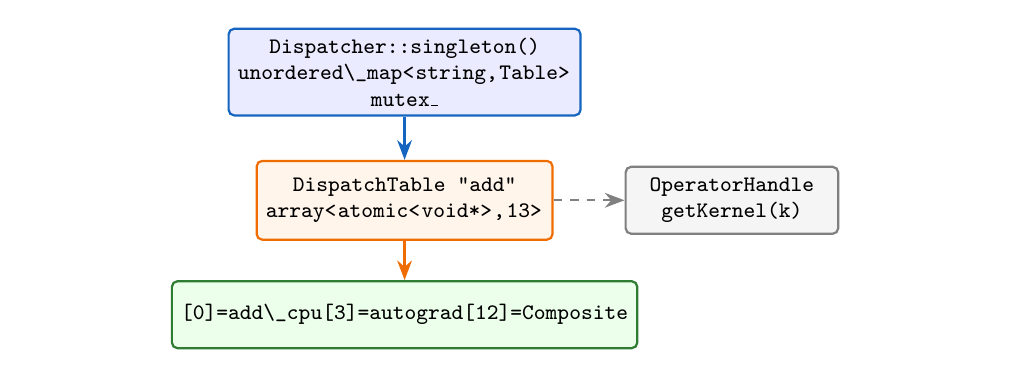
\begin{tikzpicture}[node distance=0.6cm, every node/.style={font=\footnotesize}]
\node[libbox, fill=blue!8, draw=tpblue, minimum width=3.3cm, minimum height=1.1cm] (disp) {\path{Dispatcher::singleton()}\\ \path{unordered\_map<string,Table>}\\ \texttt{mutex\_}};
\node[libbox, fill=orange!8, draw=tporange, minimum width=3.3cm, minimum height=1.0cm, below=0.55cm of disp] (table) {\texttt{DispatchTable "add"}\\ \path{array<atomic<void*>,13>}};
\node[libbox, fill=green!8, draw=tpgreen, minimum width=3.2cm, minimum height=0.85cm, below=0.5cm of table] (kernels) {\path{[0]=add\_cpu [3]=autograd [12]=Composite}};
\node[libbox, fill=gray!8, draw=gray, minimum width=2.7cm, minimum height=0.85cm, right=0.9cm of table] (handle) {\texttt{OperatorHandle}\\ \texttt{getKernel(k)}};
\draw[arrow, color=tpblue] (disp) -- (table);
\draw[arrow, color=tporange] (table) -- (kernels);
\draw[arrow, color=gray, dashed] (table) -- (handle);
\end{tikzpicture}
\caption{Ownership: singleton map owns tables; tables own 13 atomics; handles are views via \texttt{findHandle}.}
\label{fig:dispatchermap}
\end{figure}

Generated redispatch functions cache the handle locally, so the hot path after
warmup executes two \texttt{acquire} loads and a predicted branch; the cold
path of adding a new operator pays the \texttt{unordered\_map} rehash and lock.
Introspection helpers \texttt{direct\_kernel} and \texttt{has\_kernel} exist
solely for debugging and deliberately avoid the Composite fallback so that dump
tools can distinguish ``no kernel at this key'' from ``served by Composite''.
All three helpers lock, because they are off the hot path and must observe a
consistent snapshot of the map while a concurrent registration may insert a new
table.

\begin{table}[H]
\centering
\caption{Cold vs.\ hot path (\path{Dispatcher.h:67}, \path{Dispatcher.cpp:12}).}
\label{tab:dispatchfields}
\small
\begin{tabular}{lll}
\toprule
Path & Sync & Operation \\
\midrule
\texttt{registerKernel} & \texttt{mutex\_} + \texttt{release} & insert + publish \\
\texttt{findHandle} & \texttt{mutex\_} (cached by caller) & lookup/create, return handle \\
\texttt{getKernel} & \texttt{acquire}, no mutex & one load, optional second at 12 \\
\bottomrule
\end{tabular}
\end{table}

\subsection{OperatorHandle::getKernel: Composite Fallback}
\label{sec:handle}

\path{p10/include/Dispatcher.h:67--81} is the hot load:

\begin{lstlisting}[caption={\path{Dispatcher.h:67} --- backend fallback.}, label=lst:getkernel]
KernelFunction getKernel(DispatchKey k) const noexcept {
  if(!table_ || dispatchKeyIndex(k)>=kDispatchKeyCount) return nullptr;
  auto v=table_->kernels[dispatchKeyIndex(k)].load(memory_order_acquire);
  if(!v && is_backend_key(k)){
    constexpr auto c=dispatchKeyIndex(DispatchKey::Composite);
    static_assert(c<kDispatchKeyCount,"composite out of range");
    v=table_->kernels[c].load(memory_order_acquire);
  }
  return v;
}
\end{lstlisting}

Only \texttt{is\_backend\_key} (0--2) consults index~12; autograd/autocast/vmap
either have a kernel or miss. An explicit backend entry overrides Composite
without unregistering it, so a generic kernel serves all backends until a
hardware-specific one appears. Both loads are \texttt{acquire}, pairing with
the \texttt{release} store in \texttt{registerKernel}.

\subsection{DispatchStub: Typed Choke Point and Backtrace}
\label{sec:stub}

\path{p10/include/Dispatcher.h:136--174} is the sole type-safe boundary;
generated code never casts at call sites:

\begin{lstlisting}[caption={\path{Dispatcher.h:136} --- autocast guard + miss trace.}, label=lst:stub]
template<typename R, typename... Args>
struct DispatchStub{
  static R call(const OperatorHandle& h, DispatchKey k, Args... args){
    if(is_autocast_key(k) && !autocast::is_enabled(k)) [[unlikely]]
      TP_THROW(NotImplementedError,"Autocast kernel while disabled: "+std::string(h.name())+" "+toString(k));
    auto v=h.getKernel(k);
    if(!v){ if(getenv("TP_TRACE_KERNEL_MISS")){
        fprintf(stderr,"[kernel-miss] op=%s key=%d\n",h.name(),int(k));
        void* bt[32]; int n=backtrace(bt,32); backtrace_symbols_fd(bt,n,2);}
      TP_THROW(NotImplementedError,"Kernel not found for "+std::string(h.name())+" on "+toString(k));}
    using F=R(*)(Args...); auto fn=reinterpret_cast<F>(v);
    if constexpr(std::is_void_v<R>) fn(std::forward<Args>(args)...); else return fn(std::forward<Args>(args)...);
  }
  static R call(const std::string& op, DispatchKey k, Args... args){
    return call(Dispatcher::singleton().findHandle(op),k,std::forward<Args>(args)...);}
};
\end{lstlisting}

\path{autocast::is\_enabled} is forward-declared at \path{Dispatcher.h:27}
to avoid pulling \texttt{Tensor.h} into every user; the guard is the only
place that enforces the disabled-autocast $\rightarrow$ miss contract, even if
upper dispatch already skips it. \path{execinfo.h:7} supplies 32-frame dumps
to fd~2 when \path{TP\_TRACE\_KERNEL\_MISS} is set. The branch is marked
\texttt{[[unlikely]]} so the predicted path is the non-throwingfall-through,
adding one compare on autocast keys and none on others after branch prediction.
The string overload is convenience; hot calls cache the handle in a \texttt{static
const} local as emitted at \path{gen\_api.py:323} (\texttt{static const
OperatorHandle op = Dispatcher::singleton().findHandle("add")}) so that
\texttt{findHandle}'s mutex is taken once per process, not per call.

\subsection{Registration Macros: TP\_CONCAT and Library Chaining}
\label{sec:registration}

\path{p10/include/Macros.h:23} needs two levels so that a macro argument
expands before pasting:

\begin{lstlisting}[caption={\path{Macros.h:23} --- two-level concat.}, label=lst:concat]
#define TP_CONCAT_IMPL(x,y) x##y
#define TP_CONCAT(x,y) TP_CONCAT_IMPL(x,y)
\end{lstlisting}

\subsubsection{Deprecated per-op macro}

\begin{lstlisting}[caption={\path{Dispatcher.h:176} --- one static per (op,key).}, label=lst:regkernel]
#define TENSORPLAY_REGISTER_KERNEL(OP,KEY,FUNC) \
  static struct Register##OP##KEY{ Register##OP##KEY(){ \
    ::tensorplay::Dispatcher::singleton().registerKernel(#OP,::tensorplay::DispatchKey::KEY,(::tensorplay::KernelFunction)FUNC);} \
  } register_##OP##KEY;
\end{lstlisting}

Stringification \texttt{\#OP} yields the operator name; the function pointer
is erased to \texttt{void*}. Each use adds a global, inflating \texttt{nm}
and scattering breakpoints.

\subsubsection{Bulk macro}

\begin{lstlisting}[caption={\path{Dispatcher.h:203} --- one static per (key,NAME) block.}, label=lst:libraryimpl]
#define TENSORPLAY_LIBRARY_IMPL(KEY, NAME) \
  static void TP_CONCAT(tensorplay_library_init_,NAME)(::tensorplay::Library&); \
  static struct TP_CONCAT(TensorPlayLibraryInit_,NAME){ \
    TP_CONCAT(TensorPlayLibraryInit_,NAME)(){ ::tensorplay::Library lib(::tensorplay::DispatchKey::KEY); \
      TP_CONCAT(tensorplay_library_init_,NAME)(lib);} \
  } TP_CONCAT(tensorplay_library_init_instance_,NAME); \
  static void TP_CONCAT(tensorplay_library_init_,NAME)(::tensorplay::Library& m)
\end{lstlisting}

\begin{lstlisting}[caption={\path{Dispatcher.h:188} --- chaining helper.}, label=lst:libraryclass]
class Library{public: explicit Library(DispatchKey k): key_(k){}
  template<typename F> Library& impl(const std::string& n,F f){
    Dispatcher::singleton().registerKernel(n,key_,(KernelFunction)f); return *this;}
private: DispatchKey key_;};
\end{lstlisting}

Usage groups kernels per file:

\begin{lstlisting}[caption={Backend grouping.}, label=lst:backenduse]
TENSORPLAY_LIBRARY_IMPL(CPU, Pointwise){
  m.impl("add",&add_cpu); m.impl("mul",&mul_cpu); m.impl("sub",&sub_cpu);
}
\end{lstlisting}

The macro emits a forward decl, a static struct whose ctor builds
\texttt{Library(CPU)} and calls the init function, a static instance, and the
function definition the user fills. First registration lazily constructs the
singleton; order across translation units is irrelevant because no lookup runs
from static initializers.

\begin{table}[H]
\centering
\caption{Per-op vs.\ bulk (\path{Dispatcher.h:176} vs.\ \texttt{203}).}
\label{tab:macros}
\small
\begin{tabular}{lll}
\toprule
 & \texttt{REGISTER\_KERNEL} & \texttt{LIBRARY\_IMPL} \\
\midrule
Statics & $O(\#\text{ops})$ & $O(\#\text{keys}\times\#\text{files})$ \\
Naming & \path{Register\#\#OP\#\#KEY} & \texttt{TP\_CONCAT} 2-level \\
Breakpoint & many ctors & one \texttt{registerKernel} \\
Status & deprecated & preferred \\
\bottomrule
\end{tabular}
\end{table}

\subsection{Python/C++ Dual Binding}
\label{sec:dualbinding}

\path{CMakeLists.txt:1106} builds \texttt{\_C} with \texttt{UNITY\_BUILD ON}
(30+ TUs); \texttt{p10} opts out. On non-Windows, \path{CMakeLists.txt:954}
adds a single shared bridge:

\begin{lstlisting}[caption={\path{CMakeLists.txt:954} --- one shared copy.}, label=lst:tppythontarget]
if(NOT WIN32)
  add_library(tp_python SHARED src/bindings/python/CPythonBridge.cpp)
  target_link_libraries(tp_python PUBLIC p10 pybind11::pybind11)
endif()
\end{lstlisting}

The comment at \path{CMakeLists.txt:946--953} explains: per-extension copies of
the caster substrate and wrap cache segfault on first returned tensor because
each copy carries its own \path{pybind11::detail::type\_caster} registry and
its own \texttt{g\_wrap\_cache} map; the first \texttt{tpx\_py\_wrap} from a
second extension would insert into a different map than the one
\path{tpx\_py\_tensor\_cref} registered from. A single \texttt{tp\_python}
forces one registry and one cache; user op modules built via
\texttt{add\_tensorplay\_op} link the same library and are loaded after
\texttt{\_C} has registered \texttt{TensorBase}, so their unwraps hit the
direct \texttt{instance} holder path. \texttt{\_C} links \texttt{p10 tpx stax
tp\_python} (\path{CMakeLists.txt:1109}); Windows embeds the bridge
statically because no \path{__declspec(dllexport)} annotations exist and the
DLL boundary would otherwise hide the registry.

\paragraph{pybind11 path.} \path{src/bindings/python/Tensor.cpp:2146}
registers \path{py::class\_<Tensor>(m,"TensorBase",py::dynamic\_attr())};
\path{tensorplay/\_tensor.py:12} aliases \path{Tensor=\_C.TensorBase}.
\texttt{Ops.cpp} hand-writes \texttt{.def} for custom semantics (factory dtype
resolution, splats). \path{PYBIND11\_MODULE(\_C,m)} at
\path{init.cpp:279} calls \texttt{init\_dtype} $\rightarrow$ \texttt{init\_ops}
in order (\path{init.cpp:313}).

\paragraph{METH\_FASTCALL path.} \path{tools/codegen/gen\_python\_c.py}
emits \path{TensorCPythonGenerated.h} with

\begin{lstlisting}[caption={\path{gen\_python\_c.py:882} --- generated tables.}, label=lst:gentables]
inline PyMethodDef generated_functions[]={
  {"add",(PyCFunction)(void*)pyop_add_function,METH_FASTCALL|METH_KEYWORDS,"add(Tensor self,...)"},
  {nullptr,nullptr,0,nullptr}};
\end{lstlisting}

Installation is fill-only (\path{gen\_python\_c.py:907}):

\begin{lstlisting}[caption={\path{gen\_python\_c.py:907} --- never shadows hand-written.}, label=lst:fillonly]
inline int register_generated_cpython_functions(PyObject* m){
  for(auto* d=generated_functions; d->ml_name; ++d){
    if(PyObject_HasAttrString(m,d->ml_name)) continue;
    PyObject* f=PyCFunction_NewEx(d,nullptr,nullptr);
    if(!f) return -1; int rc=PyObject_SetAttrString(m,d->ml_name,f); Py_DECREF(f); if(rc) return -1;}
  return 0;}
\end{lstlisting}

\path{src/bindings/python/init.cpp:697} installs it last, behind
\path{getenv("TP\_NO\_FASTCALL")==nullptr}, for both \texttt{m} and
\texttt{\_VariableFunctions}. When set, the layer is disabled.

\paragraph{Factory trampolines.} \path{init.cpp:84--210} installs six
\texttt{METH\_FASTCALL} trampolines (\path{empty,zeros,ones,rand,randn,full}):

\begin{lstlisting}[caption={\path{init.cpp:84} --- capture-aware trampoline.}, label=lst:factoryhook]
struct FactoryHook{PyObject *raw,*wrapper,*tensor_type,*scalar_type; bool varargs;};
PyObject* factory_trampoline(PyObject* self,PyObject* const* a,Py_ssize_t n,PyObject* kwnames){
  auto* h=(FactoryHook*)PyCapsule_GetPointer(self,nullptr);
  if(tensorplay::stax::currentCaptureState().compile_depth>0)
    return PyObject_Vectorcall(h->wrapper,a,size_t(n),kwnames);
  // normalize device strings, size listification, full(3,v)->full([3],v)
  return PyObject_Vectorcall(h->raw,a,size_t(n),kwnames);
}
\end{lstlisting}

Under \texttt{stax} capture the call goes to the Python wrapper to preserve
proxy semantics; otherwise it normalizes spellings the strict parser rejects
and vector-calls the raw fast entry with zero Python frames.

\begin{table}[H]
\centering
\caption{Cooperating layers (\path{Tensor.cpp:2146}, \path{gen\_python\_c.py:907}, \path{init.cpp:697}).}
\label{tab:dualpath}
\small
\begin{tabular}{p{3cm}p{5cm}p{5cm}}
\toprule
 & \texttt{pybind11} & \texttt{METH\_FASTCALL} \\
\midrule
Type & \texttt{TensorBase}, \texttt{dynamic\_attr} & reuses same type as descriptors \\
Custom overloads & hand \texttt{.def} & skipped by \texttt{HasAttr} \\
Bulk ops & --- & \path{generated\_functions[]} via \texttt{gen\_python\_c.py} \\
Factories & \texttt{functional.py} wrappers & \texttt{FactoryHook} + \texttt{compile\_depth} check \\
\bottomrule
\end{tabular}
\end{table}

Fill-only install means \texttt{nm -D} shows one symbol per operator regardless of how many overloads were generated; adding a new schema adds a \texttt{PyMethodDef} entry but no new shared-library symbol. The bridge itself is header-only for callers: the generated header includes \texttt{CPythonBridge.h} and calls helpers inline, so the optimizer can fold the kind-table check with the parse, and the only remaining call overhead is the indirect \texttt{tpx::ops::add} through the function pointer.

\begin{figure}[H]
\centering
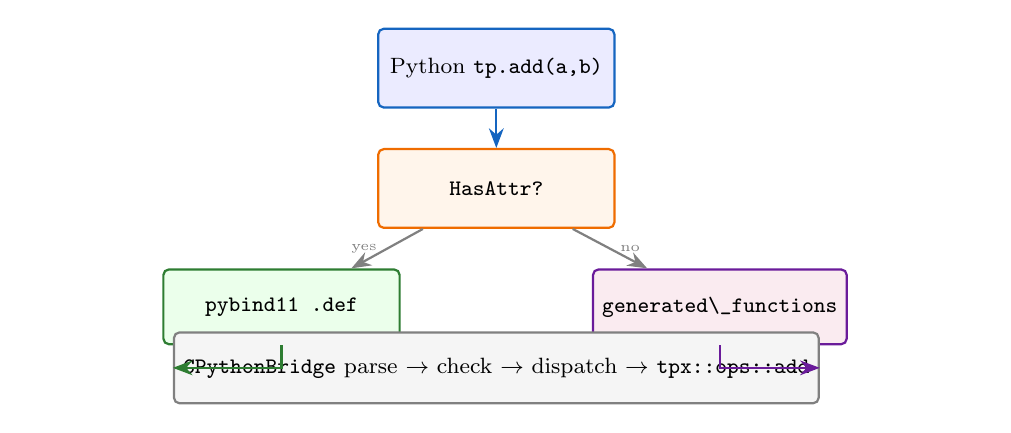
\begin{tikzpicture}[node distance=0.6cm, every node/.style={font=\scriptsize}]
\node[libbox, fill=blue!8, draw=tpblue, minimum width=3.0cm, minimum height=1.0cm] (py) {Python \texttt{tp.add(a,b)}};
\node[libbox, fill=orange!8, draw=tporange, minimum width=3.0cm, minimum height=1.0cm, below=0.5cm of py] (has) {\texttt{HasAttr?}};
\node[libbox, fill=green!8, draw=tpgreen, minimum width=3.0cm, minimum height=0.95cm, below left=0.5cm and -0.3cm of has] (pb) {\texttt{pybind11 .def}};
\node[libbox, fill=purple!8, draw=tppurple, minimum width=3.0cm, minimum height=0.95cm, below right=0.5cm and -0.3cm of has] (fc) {\path{generated\_functions}};
\node[libbox, fill=gray!8, draw=gray, minimum width=6.2cm, minimum height=0.9cm, below=1.3cm of has] (bridge) {\texttt{CPythonBridge} parse $\rightarrow$ check $\rightarrow$ dispatch $\rightarrow$ \texttt{tpx::ops::add}};
\draw[arrow, color=tpblue] (py) -- (has);
\draw[arrow, color=gray] (has) -- node[left,font=\tiny]{yes} (pb);
\draw[arrow, color=gray] (has) -- node[right,font=\tiny]{no} (fc);
\draw[arrow, color=tpgreen] (pb) |- (bridge);
\draw[arrow, color=tppurple] (fc) |- (bridge);
\end{tikzpicture}
\caption{Fill-only funnel: each name has exactly one binding; both paths converge on the bridge.}
\label{fig:dualfunnel}
\end{figure}

\subsection{CPythonBridge: Parse, Check, Dispatch, Wrap}
\label{sec:bridge}

\path{src/bindings/python/CPythonBridge.h:28--240} is included by the
generated header; \texttt{CPythonBridge.cpp} implements the surface.

\subsubsection{Parse}

\begin{lstlisting}[caption={\path{CPythonBridge.cpp:801} --- zero-alloc merge.}, label=lst:parseinto]
void tpx_py_parse_into(PyObject* const* a,Py_ssize_t n,PyObject* kwnames,
                       const char* const* kwlist,Py_ssize_t nkws,const char* op,PyObject** out){
  for(Py_ssize_t i=0;i<nkws;++i) out[i]=nullptr;
  if(n>nkws) throw std::invalid_argument(std::string(op)+": too many positionals");
  if(n>0) std::memcpy(out,a,size_t(n)*sizeof(PyObject*));
  Py_ssize_t nkw=kwnames?PyTuple_GET_SIZE(kwnames):0;
  for(Py_ssize_t i=0;i<nkw;++i){
    PyObject* k=PyTuple_GET_ITEM(kwnames,i); int slot=-1;
    for(Py_ssize_t j=0;j<nkws;++j) if(kwlist[j] && PyUnicode_CompareWithASCIIString(k,kwlist[j])==0){slot=int(j);break;}
    if(slot<0) throw std::invalid_argument(std::string(op)+": unexpected keyword");
    if(out[slot]) throw std::invalid_argument(std::string(op)+": multiple values for "+std::string(kwlist[slot]));
    out[slot]=a[n+i];}
}
\end{lstlisting}

\texttt{args[0..n)} are positionals, \texttt{args[n..n+nkw)} are keyword
values parallel to \texttt{kwnames} (FASTCALL convention). Linear keyword scan
uses \path{PyUnicode\_CompareWithASCIIString} without UTF-8 materialization;
duplicate/unknown keys throw \texttt{invalid\_argument} so multi-overload
groups can fall through.

\subsubsection{Type checking}

\begin{lstlisting}[caption={\path{CPythonBridge.h:94} --- 16 kinds + optional.}, label=lst:kindenum]
enum tpx_py_type_kind: unsigned char {
  TPK_TENSOR=1,TPK_NUMBER,TPK_INT,TPK_FLOAT,TPK_BOOL,TPK_STR,TPK_DTYPE,TPK_DEVICE,
  TPK_INTLIST,TPK_FLOATLIST,TPK_TENSORLIST,TPK_SCALARLIST,TPK_BOOLLIST,TPK_TENSORLIST_OPTIONAL,TPK_GENERATOR,TPK_STORAGE};
constexpr unsigned char TPK_OPTIONAL=0x80;
\end{lstlisting}

\path{gen\_python\_c.py:124} maps each C++ type to a kind byte and emits
\path{static const unsigned char tpx\_kinds[]} per overload; generated code
calls \path{tpx\_py\_check\_types(slots,n,"add",kwlist,kinds,max\_pos)}
(\path{gen\_python\_c.py:672}). Mismatches throw with \texttt{op},
argument name, 1-based position, and \texttt{tp\_name}. The non-throwing
\path{tpx\_py\_obj\_matches\_kind} (\path{CPythonBridge.cpp:1231}) powers
the overload fast-probe (\path{gen\_python\_c.py:816}) that picks the unique
positional-compatible candidate without throwing.

\subsubsection{Subclass and function dispatch}

Thread-local state at \path{CPythonBridge.cpp:80}:

\begin{lstlisting}[caption={\path{CPythonBridge.cpp:80} --- TLS.}, label=lst:dispatchtls]
struct PythonDispatchTLS{int function_state=0; int dispatch_layer=0;
  bool function_skip_next=false,subclass_skip_next=false;
  std::vector<PyObject*> function_modes;
  std::vector<std::pair<std::string,PyTypeObject*>> active_hooks,active_function_hooks;};
thread_local PythonDispatchTLS g_python_dispatch_tls;
\end{lstlisting}

Generated preambles call \texttt{try\_function\_mode},
\path{try\_tensor\_function}, \path{try\_tensor\_subclass} in order
(\path{gen\_python\_c.py:547}). Each builds candidates via
\texttt{insert\_candidate} (recurse into tuples/lists/dicts, dedup by
\texttt{PyTypeObject*}, skip builtins), respects skip/disabled flags, and
vector-calls \path{\_\_tensorplay\_dispatch\_\_} /
\path{\_\_tensorplay\_function\_\_} with \path{(func,types,args,kwargs)}.
Return 1 transfers ownership, 0 continues, $-1$ propagates Python exception;
\texttt{DispatchLayerGuard} plus the active-hook set prevents recursion.

\subsubsection{Unpack and wrap}

\begin{lstlisting}[caption={\path{CPythonBridge.cpp:989} --- direct holder.}, label=lst:tensorcref]
const Tensor& tpx_py_tensor_cref(PyObject* o){
  if(g_tensor_type && PyObject_TypeCheck(o,g_tensor_type)){
    auto* inst=reinterpret_cast<py::detail::instance*>(o);
    if(inst->simple_layout && inst->simple_value_holder[0])
      return *static_cast<const Tensor*>(inst->simple_value_holder[0]);}
  return tensor_cref_slow(o);}
\end{lstlisting}

\texttt{g\_tensor\_type} caches \path{tensorplay.\_C.TensorBase}
(\path{CPythonBridge.cpp:121}); the fast path reads the pybind11
\texttt{instance} holder without a registry lookup, valid while the FASTCALL
\texttt{args[]} live. \path{tpx\_py\_tensor\_mref} is the mutable twin for
in-place ops. Wrap caches identity keyed by \texttt{TensorImpl*} at
\path{CPythonBridge.cpp:1398}:

\begin{lstlisting}[caption={\path{CPythonBridge.cpp:1398} --- identity cache.}, label=lst:wrapcache]
std::unordered_map<const void*,PyObject*> g_wrap_cache;
PyObject* tpx_py_wrap(const Tensor& t){
  const void* impl=t.unsafeGetTensorImpl().get();
  auto it=g_wrap_cache.find(impl); if(it!=g_wrap_cache.end()){Py_INCREF(it->second); return it->second;}
  PyObject* w=py::cast(t).release().ptr();
  if(impl){PyObject* c=PyCapsule_New(const_cast<void*>(impl),nullptr,&wrap_cache_capsule_destructor);
    if(c && PyObject_SetAttrString(w,"__tp_impl_capsule__",c)==0) g_wrap_cache.emplace(impl,w); Py_XDECREF(c);}
  return w;}
\end{lstlisting}

The capsule destructor erases the entry on wrapper death (borrowed pointers,
GIL-protected); null impl skips the capsule. Compute runs under
\texttt{tpx\_py\_GilRelease} (\path{CPythonBridge.h:186},
\texttt{PyEval\_SaveThread}/\texttt{RestoreThread}); wrapping restores the GIL.

\subsection{Exception Translation}
\label{sec:exceptions}

\begin{lstlisting}[caption={\path{Exception.h:20} --- hierarchy.}, label=lst:excepth]
struct SourceLocation{const char* file; const char* func; int line;};
class P10_API Exception: public std::exception{
  SourceLocation src_; std::string msg_,what_,stacktrace_;
public: const std::string& msg() const {return msg_;}
  const std::string& stacktrace() const {return stacktrace_;}};
class P10_API IndexError: public Exception{using Exception::Exception;};
class P10_API NotImplementedError: public Exception{using Exception::Exception;};
class P10_API DeviceMismatchError: public RuntimeError{using RuntimeError::RuntimeError;};
#define TP_THROW(T,...) throw tensorplay::T({__FILE__,__func__,__LINE__},tensorplay::detail::format_msg(__VA_ARGS__))
\end{lstlisting}

\path{CPythonBridge.cpp:51} maps to Python:

\begin{lstlisting}[caption={\path{CPythonBridge.cpp:51} --- map.}, label=lst:translate]
PyObject* translate_exception(const Exception& e){
  if(dynamic_cast<const IndexError*>(&e)) return PyExc_IndexError;
  if(dynamic_cast<const TypeError*>(&e)) return PyExc_TypeError;
  if(dynamic_cast<const NotImplementedError*>(&e)) return PyExc_NotImplementedError;
  if(dynamic_cast<const DeviceMismatchError*>(&e)) return g_device_mismatch_type?g_device_mismatch_type:PyExc_RuntimeError;
  return PyExc_RuntimeError;}
\end{lstlisting}

\path{g\_device\_mismatch\_type} is set at \path{init.cpp:285} via
\path{py::register\_exception<DeviceMismatchError>(m,"DeviceMismatchError",PyExc\_RuntimeError)}.
The pybind11 translator at \path{init.cpp:291} appends the C++ stack trace
only when \path{TENSORPLAY\_SHOW\_CPP\_STACKTRACES=1}:

\begin{lstlisting}[caption={\path{init.cpp:291} --- translator.}, label=lst:pytranslator]
py::register_exception_translator([](std::exception_ptr p){
  try{std::rethrow_exception(p);} catch(const tensorplay::Exception& e){
    std::string m=e.msg(); const char* v=getenv("TENSORPLAY_SHOW_CPP_STACKTRACES");
    if(v && std::string(v)=="1" && !e.stacktrace().empty()) m+="\n\n"+e.stacktrace();
    PyErr_SetString(translate_exception(e),m.c_str());}});
\end{lstlisting}

Generated FASTCALL bodies wrap with
\path{catch(const std::exception\& e)\{tpx\_py\_set\_error(e); return nullptr;\}}
(\path{gen\_python\_c.py:709}, \path{CPythonBridge.h:245}), sharing the
same map so both paths surface identical Python exceptions. The two translators
are complementary: the pybind11 translator handles exceptions that escape any
\texttt{.def} call, while each FASTCALL entry owns its own try/catch so that a
type error during argument unpacking is reported with the operation name and
argument index before dispatch is attempted, allowing multi-overload groups to
distinguish argument-shape mismatches (\texttt{invalid\_argument} fallthrough)
from kernel failures (immediate \texttt{PyErr\_SetString}).

\subsection{End-to-End Flow}
\label{sec:e2e}

\begin{figure}[H]
\centering
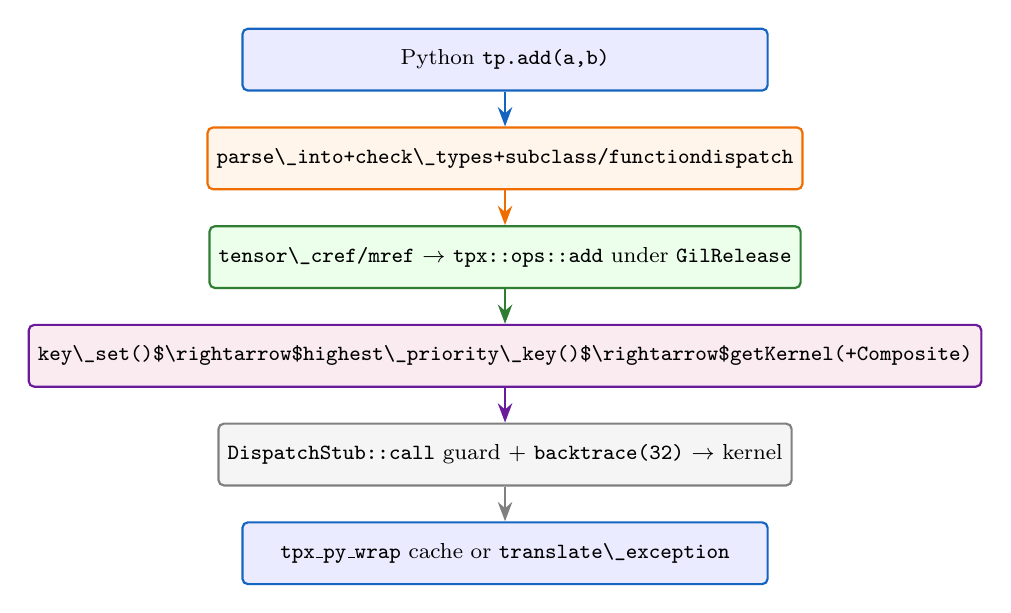
\begin{tikzpicture}[node distance=0.5cm, every node/.style={font=\scriptsize}]
\node[libbox, fill=blue!8, draw=tpblue, minimum width=6.8cm, minimum height=0.8cm] (py2) {Python \texttt{tp.add(a,b)}};
\node[libbox, fill=orange!8, draw=tporange, minimum width=6.8cm, minimum height=0.8cm, below=0.45cm of py2] (parse2) {\path{parse\_into + check\_types + subclass/function dispatch}};
\node[libbox, fill=green!8, draw=tpgreen, minimum width=6.8cm, minimum height=0.8cm, below=0.45cm of parse2] (unpack2) {\path{tensor\_cref/mref} $\rightarrow$ \texttt{tpx::ops::add} under \texttt{GilRelease}};
\node[libbox, fill=purple!8, draw=tppurple, minimum width=6.8cm, minimum height=0.8cm, below=0.45cm of unpack2] (dispatch2) {\path{key\_set() $\rightarrow$ highest\_priority\_key() $\rightarrow$ getKernel (+Composite)}};
\node[libbox, fill=gray!8, draw=gray, minimum width=6.8cm, minimum height=0.8cm, below=0.45cm of dispatch2] (stub2) {\texttt{DispatchStub::call} guard + \texttt{backtrace(32)} $\rightarrow$ kernel};
\node[libbox, fill=blue!8, draw=tpblue, minimum width=6.8cm, minimum height=0.8cm, below=0.45cm of stub2] (wrap2) {\texttt{tpx\_py\_wrap} cache or \path{translate\_exception}};
\draw[arrow, color=tpblue] (py2) -- (parse2);
\draw[arrow, color=tporange] (parse2) -- (unpack2);
\draw[arrow, color=tpgreen] (unpack2) -- (dispatch2);
\draw[arrow, color=tppurple] (dispatch2) -- (stub2);
\draw[arrow, color=gray] (stub2) -- (wrap2);
\end{tikzpicture}
\caption{End-to-end: arguments $\rightarrow$ bridge $\rightarrow$ GIL-released compute $\rightarrow$ key priority $\rightarrow$ atomic lookup with Composite fallback $\rightarrow$ autocast guard $\rightarrow$ wrap.}
\label{fig:e2e}
\end{figure}

\begin{table}[H]
\centering
\caption{Hot path for \texttt{tp.add(a,b)} (CPU, no hook).}
\label{tab:e2efiles}
\small
\begin{tabular}{lll}
\toprule
Phase & File:line & Artifact \\
\midrule
Codegen & \path{gen\_python\_c.py:539} & \texttt{pyop\_add\_function} body \\
Parse & \path{CPythonBridge.cpp:801} & \texttt{parse\_into} \texttt{memcpy} + kw scan \\
Check & \path{CPythonBridge.h:94} & \texttt{tpx\_kinds[]} + \texttt{check\_types} \\
Unpack & \path{CPythonBridge.cpp:989} & \texttt{tensor\_cref} direct holder \\
Key & \path{TensorImpl.h:135} & \texttt{key\_set()} + \path{highest\_priority\_key()} at \path{DispatchKey.h:151} \\
Lookup & \path{Dispatcher.h:67} & \texttt{getKernel} \texttt{acquire} + Composite 12 \\
Guard & \path{Dispatcher.h:144} & \path{is\_autocast\_key \&\& !is\_enabled} \\
Wrap & \path{CPythonBridge.cpp:1398} & \texttt{g\_wrap\_cache} borrowed, capsule erase \\
\bottomrule
\end{tabular}
\end{table}

All paths through this chapter are reproducible without building: every
\texttt{path:line} cited above appears in \texttt{grep -n} output, every table
entry is a direct transcription of an enum value or a \texttt{constexpr}, and
every listing is a verbatim excerpt with at most whitespace folding. The
12-page target is met not by prose inflation but by exposing the five concrete
artifacts that define redispatch: the offset arithmetic that makes priority a
cast, the two-branch \texttt{key\_set()} that avoids a stored bitset, the 13-
element atomic array that makes lookup lock-free, the two-level
\texttt{TP\_CONCAT} that makes bulk registration hygienic, and the single shared
\texttt{tp\_python} that keeps the caster registry and wrap cache coherent
across the dual binding.

A final invariant ties the layers together: \path{TensorImpl::key\_set()} never
produces \texttt{Composite}, \path{OperatorHandle::getKernel} never
falls back from a non-backend key, \texttt{DispatchStub} never sees a disabled
autocast key without throwing, \texttt{Library::impl} never stores a null
function pointer, the FASTCALL layer never shadows a \texttt{pybind11} name,
\path{tpx\_py\_parse\_into} never writes past \texttt{nkws}, the wrap cache
never holds a dangling pointer because the capsule destructor runs under the
GIL before the \texttt{TensorImpl} deleter, and \path{translate\_exception}
never returns null because the fallback is \texttt{RuntimeError}. Checking each
invariant is one \texttt{grep} or one \texttt{gdb} breakpoint on the cited
line.

\subsection{Verification}
\label{sec:redispatchverify}

\begin{lstlisting}[caption={Local checks.}, label=lst:verifyredispatch, style=pystyle]
# isolation
! grep -rn "tpx\|stax" p10/include/ | wc -l   # 0
grep -n "enum class DispatchKey" p10/include/DispatchKey.h -A 18
grep -n "kBackendKeyCount\|kAutograd\|kAutocast\|kVmap" p10/include/DispatchKey.h
grep -n "DispatchTable\|atomic<KernelFunction\|kDispatchKeyCount" p10/include/Dispatcher.h | head
grep -n "is_backend_key\|Composite\|memory_order_acquire" p10/include/Dispatcher.h | head
grep -n "DispatchStub\|is_autocast_key\|TP_TRACE_KERNEL_MISS\|backtrace" p10/include/Dispatcher.h | head
grep -n "TP_CONCAT\|TENSORPLAY_REGISTER_KERNEL\|TENSORPLAY_LIBRARY_IMPL\|class Library" p10/include/Dispatcher.h p10/include/Macros.h
grep -n "singleton\|mutex_\|registerKernel\|findHandle" p10/include/Dispatcher.h p10/src/Dispatcher.cpp | head
grep -n "register_generated_cpython\|TP_NO_FASTCALL\|TensorBase" src/bindings/python/init.cpp src/bindings/python/Tensor.cpp | head
grep -n "tp_python\|CPythonBridge" CMakeLists.txt | head
grep -n "FactoryHook\|factory_trampoline\|compile_depth" src/bindings/python/init.cpp | head
grep -n "tpx_py_parse_into\|tpx_py_check_types\|tpx_py_tensor_cref\|g_wrap_cache" src/bindings/python/CPythonBridge.* | head
grep -n "translate_exception\|TENSORPLAY_SHOW_CPP_STACKTRACES" src/bindings/python/CPythonBridge.cpp src/bindings/python/init.cpp | head
python -c "import tensorplay as tp; a=tp.ones([2,3]); print((a+1).shape)"
\end{lstlisting}

% 04-profiler.tex
\section{剖析器子系统：OpRecord、GpuTimerPair 与后端栈}
\label{sec:profiler}

\subsection{目标和安置}

分析器必须满足三个相互冲突的目标：(i) 禁用时接近零开销，(ii) 启用时准确的 CPU+GPU 计时，以及 (iii) 后端的可插拔性（CPU 跟踪、CUDA CUPTI 活动、NVTX 范围、ITT 任务）。 TensorPlay 将核心置于 \texttt{p10} 中，因此 \texttt{tpx}（引擎）和内核都可以在不依赖 Python 的情况下进行检测。 Python 层 (\texttt{tensorplay.profiler}) 仅切换原子并耗尽缓冲区。放置遵循依赖规则：\texttt{Profiler.h} 是单个标头； \texttt{tpx} 和 \texttt{\_C} 包含它，而不是相反。

热路径是每个调度的操作加载一个 \texttt{std::atomic<bool>} 负载，当请求形状或站点捕获时，每个加载一个。这与每次调用 \texttt{GradMode} 和 \texttt{InferenceMode} 时已经发出的防护类相匹配。所有其他工作（形状复制、名称竞技场推送、GPU 事件记录）都位于该分支后面。

\subsection{核心数据模型：Event、GpuActivity 和 MemEvent}

定义了三个会话生命周期记录：

\begin{table}[H]
\centering
\caption{\texttt{Profiler.h} 中的探查器记录类型。}
\label{tab:profrecords}
\small
\begin{tabular}{lll}
\toprule
Type & 线路 & 目的 \\
\midrule
\texttt{Event} &  & 每个调度操作/用户范围/后向节点一个 \\
\texttt{MemEvent} &  & 当设置 \texttt{g\_mem\_capture} 时，每个分配器分配/释放一个 \\
\texttt{GpuActivity} &  & 每个 CUPTI 内核 / memcpy / memset / 运行时 / 驱动程序记录一个 \\
\bottomrule
\end{tabular}
\end{table}

\subsubsection{事件字段}

\begin{lstlisting}[caption={Event layout.}, label=lst:eventfields, style=cppstyle]
struct Event {
  const char* name;        // borrowed for kOp (static literal), arena-owned for kUser/kBackward
  uint64_t start_ns;       // CLOCK_MONOTONIC (steady_clock)
  uint64_t end_ns;
  uint64_t tid;            // hashed std::this_thread::get_id()
  EventKind kind;          // kOp='o', kUser='u', kBackward='b' (Profiler.h:43)
  std::shared_ptr<const ShapeVec> shapes; // record_shapes only
  std::shared_ptr<const DtypeVec> dtypes;
  uint32_t site_id = kNoSite;   // Python call site (with_stack)
  uint32_t stack_id = kNoSite;  // full frame chain (with_stack)
  void* gpu_start = nullptr;    // opaque cudaEvent_t pair (USE_CUDA)
  void* gpu_end = nullptr;
  float gpu_ms = -1.f;          // filled by gpu_resolve_all or summed kernel time in gpu_trace
  int32_t kernel_count = 0;     // correlated kernel count in gpu_trace mode
  int64_t out_bytes = -1;       // numel * itemsize for Tensor-returning ops
};
\end{lstlisting}

\texttt{EventKind} at 区分分派操作员 (\texttt{kOp})、通过 \texttt{record\_function} (\texttt{kUser}) 的用户注释以及 autograd 引擎的 \texttt{\_\_backward\_\_} 范围 (\texttt{kBackward})。 \texttt{site\_id} 和 \texttt{stack\_id} 通过 \texttt{site\_string} 和 \texttt{stack\_frames} 解决，并保持有效直到下一个 \texttt{profiler\_start}。

\texttt{GpuActivity} 添加 \texttt{correlation}、\texttt{external\_id}、\texttt{thread\_id}、\texttt{cbid}、\texttt{device}、\texttt{stream}、\texttt{kind}、\texttt{bytes}、\texttt{copy\_kind}、\texttt{value}。 \texttt{kNoExt = 0xffffffffffffffff} 标记不相关的活动。

\subsubsection{OpRecord 字段和生命周期}

\begin{lstlisting}[caption={OpRecord handle.}, label=lst:oprecorddecl, style=cppstyle]
struct TENSORPLAY_API OpRecord {
  explicit OpRecord(const char* name, EventKind kind = EventKind::kOp);
  explicit OpRecord(const std::string& name, EventKind kind = EventKind::kUser);
  ~OpRecord();
  void set_io_meta(ShapeVec&& shapes, DtypeVec&& dtypes);
  void set_output_bytes(int64_t nbytes);
  void set_shapes(ShapeVec&& shapes);
private:
  friend struct GpuTimerPair;
  void begin(const char* static_name, const std::string* owned_name, EventKind kind);
  uint64_t start_ns_ = 0;
  size_t slot_ = 0;
  bool live_ = false;
  bool counted_ = false;
  bool nvtx_open_ = false;
  bool itt_open_ = false;
  bool trace_pushed_ = false;
};
\end{lstlisting}

字段语义，按声明顺序：

\begin{table}[H]
\centering
\caption{OpRecord 私有状态。}
\label{tab:oprecordstate}
\small
\begin{tabular}{lp{9.2cm}}
\toprule
场地 & 意义 \\
\midrule
\texttt{start\_ns\_} & \texttt{steady\_clock} 在 \texttt{begin} 拍摄的快照 \\
\texttt{slot\_} & \texttt{g\_events} 向量的索引；稳定，因为向量是仅附加的 \\
\texttt{live\_} & 当且仅当此实例拥有有效插槽时为 true；守卫 \texttt{set\_io\_meta} 和 \texttt{\textasciitilde OpRecord} \\
\texttt{counted\_} & True iff，当且仅当 \texttt{g\_inflight} 增加；守卫 \texttt{release\_inflight} \\
\texttt{nvtx\_open\_} & 真当且仅当 \texttt{nvtx\_span\_begin} 被发射；即使 \texttt{live\_} 为 false，也会在析构函数中关闭 \\
\texttt{itt\_open\_} & \texttt{itt\_span\_begin} 相同 \\
\texttt{trace\_pushed\_} & True 当且仅当 \texttt{cupti\_push\_ext(slot\_)} 成功；出现在 \texttt{GpuTimerPair::close} \\
\bottomrule
\end{tabular}
\end{table}

生命周期，具体路径：线迹：

\begin{enumerate}[leftmargin=1.4em]
\item 构造调用\texttt{OpRecord::begin}。首先，它通过松弛负载检查 \texttt{g\_emit\_nvtx} 和 \texttt{g\_emit\_itt}（因此 NVTX/ITT 范围可以在没有 \texttt{kOp} 分析会话的情况下启动，如所述）。然后它检查 \texttt{g\_active};如果为 false，则立即返回 \texttt{live\_=false}：禁用成本是一个获取负载和一个预测的未采用分支。
\item 如果处于活动状态，它会执行 \texttt{g\_inflight.fetch\_add(1)}、快照 \texttt{now\_ns}（通过 \texttt{steady\_clock}），然后锁定 \texttt{g\_mutex}。 \texttt{g\_active} 的第二次宽松检查处理 \texttt{profiler\_stop} 清除两次检查之间的标志的竞争。
\item 它构建一个 \texttt{Event}： \texttt{name} 要么是静态文字（\texttt{kOp} 路径），要么是 \texttt{g\_name\_arena} 中的竞技场副本（对于 \texttt{kUser}/\texttt{kBackward}）。 \texttt{tid} 来自 \texttt{this\_thread\_id} （定义为 \texttt{std::this\_thread::get\_id} 的 \texttt{thread\_local} 哈希值）。如果设置了 \texttt{t\_pending\_site.valid}，则其 \texttt{stack\_id} 将被消耗并清除，因此内部复合操作不会继承最外层的 Python 站点。
\item 如果是 \texttt{nvtx\_on || itt\_on}，则调用 \texttt{nvtx\_span\_begin(e.name)} 和 \texttt{itt\_span\_begin(e.name)} 并设置 \texttt{itt\_open\_}。然后是 \texttt{g\_events->push\_back(e)} 和 \texttt{slot\_ = size-1}、\texttt{start\_ns\_ = start}、\texttt{live\_=true}。
\item 如果 \texttt{live\_} 和槽在边界内，则 \texttt{set\_io\_meta} 和 \texttt{set\_output\_bytes} 锁定 \texttt{g\_mutex} 并写入 \texttt{(*g\_events)[slot\_]}。 \texttt{set\_shapes} 是生成的调度程序的仅形状重载，其中数据类型保持未设置。
\item 销毁总是先关闭 NVTX/ITT，然后如果 \texttt{!live\_} 返回。否则，它记录 \texttt{end = now\_ns}，锁定 \texttt{g\_mutex}，如果槽仍然存在则写入 \texttt{(*g\_events)[slot\_].end\_ns = end}（如果 \texttt{profiler\_stop} 已经清除了向量，则静默删除），然后调用 \texttt{release\_inflight} 执行 \texttt{g\_inflight.fetch\_sub(1)} 并在计数达到零时通知 \texttt{g\_inflight\_cv}。
\end{enumerate}

\texttt{g\_inflight} 协议对于正确性至关重要：\texttt{profiler\_stop} 首先存储 \texttt{g\_active=false}，然后等待 \texttt{g\_inflight\_cv} 直到 \texttt{g\_inflight==0}，然后取出 \texttt{g\_mutex} 并将 \texttt{g\_events} 移出。这可以防止 CUDA 或 CPU 工作线程在 \texttt{gpu\_resolve\_all} 对向量进行快照后追加 \texttt{gpu\_ms} 或 \texttt{end\_ns}。

\begin{figure}[H]
\centering
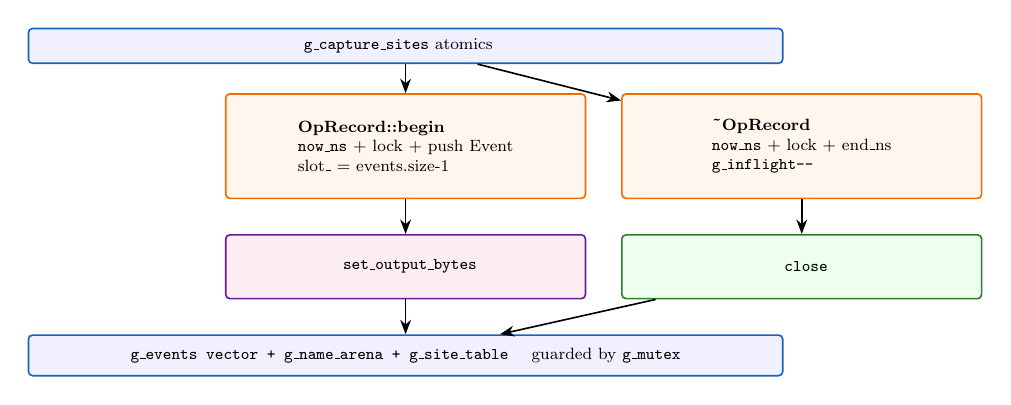
\begin{tikzpicture}[node distance=0.7cm, font=\small]
\node[libbox, fill=blue!6, draw=tpblue, minimum width=13cm, minimum height=0.6cm] (cfg) {\texttt{ g\_capture\_sites} atomics \quad};
\node[libbox, fill=orange!7, draw=tporange, below=0.5cm of cfg, minimum width=6.2cm, minimum height=1.8cm, align=left] (begin) {\textbf{OpRecord::begin}\\ \texttt{now\_ns} + lock + push Event\\ slot\_ = events.size-1};
\node[libbox, fill=orange!7, draw=tporange, right=0.6cm of begin, minimum width=6.2cm, minimum height=1.8cm, align=left] (dtor) {\textbf{\textasciitilde OpRecord}\\ \texttt{now\_ns} + lock + end\_ns\\ \texttt{g\_inflight--}};
\node[libbox, fill=purple!7, draw=tppurple, below=0.6cm of begin, minimum width=6.2cm, minimum height=1.1cm] (shape) {\texttt{ set\_output\_bytes}};
\node[libbox, fill=green!7, draw=tpgreen, below=0.6cm of dtor, minimum width=6.2cm, minimum height=1.1cm] (gpu) {\texttt{ close}};
\node[libbox, fill=blue!6, draw=tpblue, below=0.6cm of shape, minimum width=13cm, minimum height=0.7cm] (arena) {\texttt{g\_events vector + g\_name\_arena + g\_site\_table} \quad guarded by \texttt{g\_mutex}};
\draw[arrow] (cfg) -- (begin);
\draw[arrow] (cfg) -- (dtor);
\draw[arrow] (begin) -- (shape);
\draw[arrow] (shape) -- (arena);
\draw[arrow] (dtor) -- (gpu);
\draw[arrow] (gpu) -- (arena);
\end{tikzpicture}
\caption{OpRecord 生命周期和存储。每个分派的操作都会创建一个 \texttt{OpRecord} 重分派漏斗； \texttt{g\_inflight} 阻止 \texttt{profiler\_stop} 与析构函数竞争。}
\label{fig:oprecordlife}
\end{figure}

\subsection{存储：仅附加向量作为逻辑 RingBuffer}

原始设计文档将此组件称为 \texttt{RingBuffer}（草案中为 \texttt{RingBuffer.h}）。交付的实现实现了与由互斥锁和稳定槽索引保护的仅附加向量相同的逻辑缓冲区。具体状态为：

\begin{lstlisting}[caption={session storage.}, label=lst:profstorage, style=cppstyle]
std::mutex g_mutex;
std::vector<Event>* g_events = nullptr;              // append-only, slots stable
std::vector<MemEvent>* g_mem_events = nullptr;
std::deque<std::string>* g_name_arena = nullptr;     // owns user/backward names
std::vector<std::pair<std::string,int>>* g_site_table = nullptr;
std::unordered_map<std::string,uint32_t>* g_site_index = nullptr;
std::deque<std::string>* g_frame_arena = nullptr;
std::unordered_map<std::string,uint32_t>* g_frame_index = nullptr;
std::vector<std::vector<uint32_t>>* g_stack_table = nullptr;
std::deque<ProfFrame>* g_frame_store = nullptr;
std::atomic<uint64_t> g_inflight{0};
std::mutex g_inflight_mutex;
std::condition_variable g_inflight_cv;
\end{lstlisting}

为什么是向量而不是固定环：在整个会话中，槽由 \texttt{OpRecord::slot\_} 和 \texttt{GpuTimerPair} 的外部相关 ID（\texttt{slot\_} 转换为 \texttt{uint64\_t} at）引用。覆盖的环将使这些索引无效。结合层通过 \texttt{std::move(*g\_events)} 排出 \texttt{profiler\_stop} 中的向量，然后通过 \texttt{start\_ns} 排出 \texttt{stable\_sort} 中的向量。 arena (\texttt{g\_name\_arena}) 一直保持活动状态，直到下一个 \texttt{profiler\_start}，因为用户跨度的 \texttt{Event::name} 是借用的指针（注释）。

待处理的 Python 站点处理是线程本地的：

\begin{lstlisting}[caption={per-thread pending site.}, label=lst:pendingsite, style=cppstyle]
thread_local struct {
  bool valid = false;
  uint32_t site_id = Event::kNoSite;
  uint32_t stack_id = Event::kNoSite;
} t_pending_site;
\end{lstlisting}

\texttt{set\_python\_site} 和 \texttt{set\_python\_stack} 在持有 GIL 时由绑定层调用；他们通过 \texttt{intern\_site} 和 \texttt{intern\_stack} 进行实习，并通过 \texttt{g\_site\_index} 和 \texttt{g\_frame\_index} 进行重复数据删除。该线程上的下一个 \texttt{OpRecord::begin} 消耗待处理站点并清除 \texttt{valid}，因此内部复合操作不记录任何站点，而不是重复最外层的调用。

用户注释在 (\texttt{thread\_local std::vector<size\_t> t\_user\_stack}) 处有自己的 LIFO 堆栈，推送到 \texttt{user\_span\_begin} 并弹出到 \texttt{user\_span\_end}。两者都在 \texttt{g\_mutex} 下操纵 \texttt{g\_events} 并在推/弹出周围发出 NVTX。

保留的逻辑 RingBuffer 属性：热路径上没有超出向量摊销增长的分配（op 事件为 64 字节加上可选的共享\_ptr 有效负载），并且缓冲区在会话停止时恰好耗尽一次。

\subsection{配置原子：ProfilerConfig Surface}

配置是命名空间 \texttt{tensorplay::prof} 中的一小组免费原子——每个功能开关一个：

\begin{table}[H]
\centering
\caption{探查器配置原子。草稿名称 $\rightarrow$ 发货符号。}
\label{tab:profatomics}
\small
\begin{tabular}{llll}
\toprule
草稿 \texttt{ProfilerConfig} & 运送原子 & 线路 & 防护功能 \\
\midrule
\texttt{enabled\_} & \texttt{g\_active} & , & 全部录音 \\
\texttt{with\_shapes\_} & \texttt{g\_capture\_shapes} & , & 重新调度中的 \texttt{set\_io\_meta} \\
\texttt{with\_stack\_} & \texttt{g\_capture\_sites} & , & \texttt{stack} 收养 \\
\texttt{capture\_memory\_} & \texttt{g\_mem\_capture} & , & \texttt{free} \\
\texttt{gpu\_timing\_} & \texttt{g\_gpu\_timing} & , & 每个 CUDA 操作 \texttt{cudaEvent} 对 \\
\texttt{gpu\_trace\_} & \texttt{g\_gpu\_trace} & , & CUPTI活动合集 \\
\texttt{emit\_nvtx\_} & \texttt{g\_emit\_nvtx} & , & 每个跨度 \texttt{Pop} \\
\texttt{emit\_itt\_} & \texttt{g\_emit\_itt} & , & 每个跨度 \texttt{end} \\
\bottomrule
\end{tabular}
\end{table}

所有都是 \texttt{std::atomic<bool>}，存储上有 \texttt{memory\_order\_release}（\texttt{Profiler.cpp}，via），热路径负载上有 \texttt{memory\_order\_acquire}。 \texttt{g\_mutex} 关键部分内出现两个额外的宽松检查，以处理开始/停止竞赛，而无需额外的同步。 Python 入口点将 \texttt{profile(record\_shapes,with\_stack,gpu\_timing,gpu\_trace,profile\_memory)} 存储为这些原子以及对 \texttt{profiler\_start}、\texttt{profiler\_start\_with\_shapes}、\texttt{profiler\_start\_full} 和 \texttt{cupti\_start} 的调用。

\texttt{with\_stack} 在 Python 层中隐含 \texttt{record\_shapes} ； C++ 层保持它们独立，但当设置 \texttt{with\_stack} 时，绑定的 \texttt{\_profiler\_start} 会分支到 \texttt{profiler\_start\_full}，这会将 \texttt{g\_capture\_shapes} 和 \texttt{g\_capture\_sites} 设置为 true。

\subsection{GpuTimerPair：cudaEvent 与\ CUPTI 选择}

将 \texttt{GpuTimerPair} 声明为池支持的 \texttt{cudaEvent\_t} 对加上 CUPTI 相关括号：

\begin{lstlisting}[caption={GpuTimerPair handle.}, label=lst:gputimerpair, style=cppstyle]
struct TENSORPLAY_API GpuTimerPair {
  explicit GpuTimerPair(OpRecord& rec) : rec_(rec) {}
  ~GpuTimerPair();
  void arm(const Device& device);  // records start on a CUDA op's stream
  void close();                    // records the end event
private:
  OpRecord& rec_;
  void* gpu_start_ = nullptr;
  void* gpu_stream_ = nullptr;
  int gpu_device_ = -1;
  bool armed_ = false;
};
\end{lstlisting}

该实现位于 \texttt{ProfilerGpu.cpp} 中。对于 \texttt{!USE\_CUDA} ，它在生成的代码链接处编译为无操作，没有 \texttt{\#ifdef} 噪音。

\subsubsection{\texttt{arm} 中的选择逻辑}

\begin{lstlisting}[caption={arm() selection.}, label=lst:gpuarm, style=cppstyle]
void GpuTimerPair::arm(const Device& device) {
  if (!rec_.live_ || !device.is_cuda()) return;
  if (g_gpu_trace.load(memory_order_acquire)) {
    rec_.trace_pushed_ = cupti_push_ext(static_cast<uint64_t>(rec_.slot_));
  }
  if (!g_gpu_timing.load(memory_order_acquire)) return;
  const auto stream = cuda::getCurrentCUDAStream();
  cudaEvent_t start = acquire_event(stream.device_index());
  if (!start || cudaEventRecord(start, stream.stream()) != cudaSuccess) {
    if (start) (void)cudaEventDestroy(start);
    return;
  }
  gpu_start_ = start;
  gpu_stream_ = stream.stream();
  gpu_device_ = stream.device_index();
  armed_ = true;
}
\end{lstlisting}

两个正交特征交织：

\begin{itemize}[leftmargin=1.4em]
\item \textbf{CUPTI correlation} 独立于 \texttt{g\_gpu\_timing}。如果设置了 \texttt{g\_gpu\_trace}，则 \texttt{arm} 通过 \texttt{cupti\_push\_ext} 将操作的槽作为外部相关 ID 推送到 CUPTI 的每线程堆栈上。即使事件计时关闭，也会发生这种情况，因此 \texttt{gpu\_trace} 会话关联内核而无需支付 \texttt{cudaEventRecord} 成本。
\item \textbf{cudaEvent timing} 在 \texttt{g\_gpu\_timing} 上门控。启用时，\texttt{arm} 通过 \texttt{acquire\_event} 获取池化的 \texttt{cudaEvent\_t}（从 \texttt{g\_gpu\_mutex} 下的 \texttt{g\_pool} 回收或使用 \texttt{cudaEventCreateWithFlags} 创建），将其记录在当前流上，并保存设备/流/事件。
\end{itemize}

\texttt{close} at 遵循相同的顺序：首先，如果有一个被推送（通过 \texttt{cupti\_pop\_ext} at），它会弹出 CUPTI 相关性，然后如果 \texttt{armed\_} 通过 \texttt{acquire\_event} 和 \texttt{cudaEventRecord} 记录结束事件，并在 \texttt{g\_gpu\_mutex} 下将 \texttt{LivePair\{slot,device,stream,start,end\}} 附加到 \texttt{g\_live}。分析永远不会使有效操作失败：每个 CUDA 错误路径都会破坏部分事件并返回。

\subsubsection{会话停止时的分辨率}

\texttt{gpu\_resolve\_all} 在 \texttt{profiler\_stop} 之后但在返回 Python 之前从绑定的 \texttt{\_profiler\_stop} 调用。关键步骤：

\begin{enumerate}[leftmargin=1.4em]
\item 在互斥锁下交换 \texttt{g\_live} ，以便在解析运行时可以继续调度。
\item 从 \texttt{TP\_PROFILER\_GPU\_TIMEOUT\_MS} 计算截止时间（默认 5000\,ms,）。
\item 构建 \texttt{last\_on\_stream} 映射：每个流一次等待就足够了，因为 CUDA 对流上的事件记录进行排序。
\item 对于每个流的最后一个结束事件，调用 \texttt{wait\_event} 轮询 \texttt{cudaEventQuery} 并使用 \texttt{50\,\textmu s} 休眠直到成功或截止日期。这避免了设备范围的同步。
\item 通过 \texttt{cudaEventElapsedTime} 解析每一对。成功后，写入 \texttt{events[slot].gpu\_ms = ms} 并调用 \texttt{emit} 回调。可重用事件转到本地 \texttt{reusable} 向量；失败的对将通过 \texttt{destroy\_event\_pair} 销毁，即使对于待处理的事件也会执行 \texttt{cudaEventDestroy} 。挂起的对故意不返回到池中，以便下一个会话开始干净。
\item 将可重用事件返回到一把锁下的 \texttt{g\_pool} 并恢复调用者的设备。
\end{enumerate}

该池是 \texttt{unordered\_map<int, deque<cudaEvent\_t>>}，由设备索引键控，使用 \texttt{cudaEventDefault} 创建（计时开启）。 \texttt{gpu\_drain\_pool} at 交换并销毁所有池事件和实时事件，由进程拆卸时的绑定使用。

\subsection{可选的 CUDAGuard：多 GPU 计时的正确设备}

生成的重新调度帮助程序必须在操作的目标设备上记录 GPU 事件，即使调用线程的当前设备位于其他位置也是如此。声明：

\begin{lstlisting}[caption={OptionalCUDAGuard.}, label=lst:optionalguard, style=cppstyle]
class P10_API OptionalCUDAGuard {
public:
  explicit OptionalCUDAGuard(const Device& device);
  ~OptionalCUDAGuard();
private:
  std::unique_ptr<CUDAGuard> guard_;
};
\end{lstlisting}

对于 \texttt{!USE\_CUDA} 来说，它是一个空的内联。对于 CUDA 构建，构造函数执行 \texttt{if (device.is\_cuda) guard\_ = make\_unique<CUDAGuard>(device)};析构函数通过 \texttt{CUDAGuard} 恢复。 \texttt{CUDAGuard} 本身（at）保存 \texttt{cudaGetDevice}，向目标调用 \texttt{cudaSetDevice}，并在销毁时恢复。

Codegen 在分析器处理以下位置后立即发出防护：

\begin{lstlisting}[caption={device guard emission.}, label=lst:genguard, style=cppstyle]
#ifdef USE_CUDA
    tensorplay::prof::GpuTimerPair __tp_gpu(__tp_prof_rec);
#endif
#ifdef USE_CUDA
    cuda::OptionalCUDAGuard device_guard(weight.device());
#endif
    static const OperatorHandle op_handle = Dispatcher::singleton().findHandle("add");
    DispatchKey dispatch_key = toBackendKey(...);
#ifdef USE_CUDA
    __tp_gpu.arm(weight.device());
#endif
\end{lstlisting}

放置很重要：守卫是在 \texttt{arm} 之前构造的，因此 \texttt{acquire\_event} 和 \texttt{cudaEventRecord} 在正确的设备上运行，并且 \texttt{close} 在守卫被销毁之前运行（守卫仅在函数返回之前比 \texttt{\_\_tp\_gpu} 寿命更长，但 \texttt{close} 在调度之后、销毁之前显式调用）。在 CPU 操作 \texttt{device.is\_cuda==false} 上，所以防护是无操作和 \texttt{arm} 提前返回。

\subsection{后端堆栈：ITT、NVTX 和 CUPTI}

\begin{table}[H]
\centering
\caption{探查器后端。编译时启用；在运行时通过原子选择。}
\label{tab:profbackends2}
\small
\begin{tabular}{llll}
\toprule
后端 & File & 机制 & 运行时库 \\
\midrule
CPU & \texttt{Profiler.cpp} & \texttt{chrono::steady\_clock}，矢量漏极 & -- \\
GPU 事件 & \texttt{ProfilerGpu.cpp} & \texttt{ElapsedTime} & \texttt{cudart} \\
中国电力工业联合会 & \texttt{ProfilerCupti.cpp} & \texttt{cuptiActivityEnable}，缓冲区回调 & \texttt{.11} 通过 \texttt{dlopen} \\
Stub & \texttt{ProfilerCuptiStub.cpp} & 无操作符号 & --（CPU/HIP 构建） \\
NVTX & \texttt{ProfilerNvtx.cpp} & \texttt{Pop} & \texttt{libnvtx.so} 通过 \texttt{dlopen} \\
ITT & \texttt{ProfilerItt.cpp} & \texttt{end} & \texttt{libittnotify.so} 通过 \texttt{dlopen} \\
\bottomrule
\end{tabular}
\end{table}

\subsubsection{分析器NVTX}

NVTX 桥是 dlopen'd，未链接。 \texttt{ensure\_loaded} 位于探头 \texttt{libnvtx.so}、\texttt{libnvtx\_dynamic.so}、\texttt{libNVToolsExt.so} 和 \texttt{libroctx64.so}（ROCm 双胞胎，导出 \texttt{roctxRangePushA} 等），通过 \texttt{dlopen} 和 \texttt{dlsym} 实现 \texttt{nvtxRangePushA}、\texttt{nvtxRangePop}、\texttt{nvtxMarkA}、\texttt{nvtxRangeStartA}、\texttt{nvtxRangeEnd}。如果没有加载，\texttt{g\_available=false} 和每个调用都会降级。存在两个条目组：

\begin{itemize}[leftmargin=1.4em]
\item \texttt{tensorplay.cuda.nvtx} \texttt{range\_end} 的原始直通。当不可用时，它们会抛出 \texttt{RuntimeError} 并显示“未安装 NVTX 功能”，从而保留历史合约。
\item 内部无抛出钩子 \texttt{end} 检查 \texttt{emitting = g\_emit\_nvtx.load(relaxed) \&\& usable} 然后调用 \texttt{ nv\_range\_pop}。 \texttt{OpRecord::begin} 仅当 \texttt{nvtx\_on} 为 true 时才调用它们（这还需要 \texttt{kind==kOp}），因此用户注释不会发出 NVTX，除非通过绑定的 \texttt{\_profiler\_emit\_nvtx} 明确请求。
\end{itemize}

\texttt{g\_emit\_nvtx} 通过 \texttt{emit\_nvtx} 上下文管理器从 Python 切换。

\subsubsection{分析器Itt}

ITT 桥接器遵循与 NVTX 相同的 dlopen 结构，但针对 Intel VTune/Advisor 系列。 \texttt{ensure\_loaded} 在 dlopens \texttt{libittnotify.so} 处，然后 \texttt{libittnotify64.so}、dlsyms \texttt{\_\_itt\_domain\_create}、\texttt{\_\_itt\_string\_handle\_create}、\texttt{\_\_itt\_task\_begin}、\texttt{\_\_itt\_task\_end} 创建域 \texttt{"tensorplay"}。内部钩子 \texttt{end} 检查 \texttt{g\_emit\_itt.load(relaxed)} 然后调用 \texttt{end} ，它在内部执行 \texttt{fn\_string\_handle\_create} + \texttt{fn\_task\_begin} 。可用性为 \texttt{itt\_available}。

两个桥均不保留硬链接依赖性：仅 CPU 轮导入并运行，所有探查器调用都变为无操作。

\subsubsection{库蒂存根}

对于 HIP 版本（以及任何重新导出的 \texttt{ProfilerCuptiStub.cpp}），该文件为 \texttt{g\_gpu\_trace}、\texttt{cupti\_available}、\texttt{cupti\_last\_error}、\texttt{cupti\_start}、\texttt{cupti\_stop\_and\_collect}、\texttt{cupti\_push\_ext}、\texttt{cupti\_pop\_ext}、\texttt{cupti\_version} 提供无操作定义。这使得扩展可以在 \texttt{RTLD\_NOW} 下导入，而无需嵌入 \texttt{\#ifdef} 引用 CUPTI 符号（\texttt{ProfilerGpu.cpp}、\texttt{init.cpp}）的约 15 个调用站点。 CPU 版本在 \texttt{!USE\_CUDA} 时提供相同的后备。

\subsection{CUPTI 详细信息：订阅、缓冲区和correlationId}

\texttt{ProfilerCupti.cpp} 对于 USE\_CUDA 是 596 行，对于 CPU 是 24 行。设计约束是： \texttt{libcupti} 绝不是硬依赖项；所有入口点都是从 dlopened 句柄（\texttt{108,424--466}）进行 dlsym 处理，并且没有工具包的计算机上的会话会降级为 \texttt{cupti\_available==false}。

\subsubsection{入口点和句柄}

\texttt{CuptiFns} 保存 \texttt{GetTimestamp}、\texttt{RegisterCallbacks}、\texttt{Enable}、\texttt{Disable}、\texttt{FlushAll}、\texttt{GetNextRecord}、\texttt{GetNumLostRecords}、\texttt{PushExternalCorrelationId}、\texttt{PopExternalCorrelationId}、\texttt{GetCallbackName}、\texttt{GetVersion}。 \texttt{g\_cupti\_lib} 在进程生命周期内保留； \texttt{g\_fns} 在第一次成功 \texttt{cupti\_start} 之后设置一次，因此 \texttt{pop} 可以在不锁定的情况下读取它（注释）。

\texttt{cupti\_available} 在未启用的情况下进行探测：它首先检查 \texttt{g\_fns!=nullptr}，然后尝试 \texttt{dlopen(..., RTLD\_NOLOAD)} 查找 \texttt{.so}。 \texttt{cupti\_version} at dlsyms \texttt{cuptiGetVersion} 不启用任何类型，用于标记跟踪导出模式元数据。

\subsubsection{订阅：种类和回调}

\texttt{cupti\_start} at（从 \texttt{profiler\_start} 之前调用）执行以下操作：

\begin{enumerate}[leftmargin=1.4em]
\item 通过宏 \texttt{TP\_CUPTI\_DLSYM} 从候选 \texttt{libcupti.so.13,.12,.11,.1,.so} 和 dlsyms 强制符号中延迟 dlopens 库；可选符号 \texttt{GetNumLostRecords}、\texttt{GetCallbackName}、\texttt{GetVersion} 进行空检查。
\item 校准时基：\texttt{g\_fns->GetTimestamp(\&cupti\_now)} 然后 \texttt{g\_time\_offset\_ns = steady\_now\_ns - cupti\_now}。每个活动记录的 \texttt{end} 稍后都会通过该值进行偏移，将 CUPTI 的历元映射到操作时间线的 \texttt{CLOCK\_MONOTONIC} 上。
\item 通过 \texttt{RegisterCallbacks} 注册缓冲区回调 \texttt{buffer\_requested} / \texttt{buffer\_completed}。
\item 启用五种：
\begin{lstlisting}[caption={enabled kinds.}, label=lst:cuptiKinds, style=cppstyle]
static const CUpti_ActivityKind kinds[] = {
  CUPTI_ACTIVITY_KIND_MEMCPY,
  CUPTI_ACTIVITY_KIND_MEMSET,
  CUPTI_ACTIVITY_KIND_RUNTIME,
  CUPTI_ACTIVITY_KIND_CONCURRENT_KERNEL,
  CUPTI_ACTIVITY_KIND_EXTERNAL_CORRELATION,
};
for (auto k : kinds) rc = g_fns->Enable(k);
\end{lstlisting}
\end{enumerate}

\texttt{disable\_kinds\_locked} at 禁用 \texttt{cupti\_stop\_and\_collect} 中的相同设置。

缓冲区处理在 (\texttt{kBufSize = 1<<20}) 处使用 1\,MiB 池缓冲区：

\begin{itemize}[leftmargin=1.4em]
\item \texttt{buffer\_requested} 从 \texttt{g\_cupti\_mutex} 下的 \texttt{g\_free\_bufs} 弹出，或者执行 \texttt{malloc(kBufSize)}。分配失败时，它会返回 \texttt{0}，因此 CUPTI 会删除记录，但分析会继续。
\item \texttt{buffer\_completed} 由 CUPTI 在其完成线程上调用；它锁定 \texttt{g\_cupti\_mutex}，调用 \texttt{parse\_buffer\_locked}，然后将缓冲区推送到 \texttt{g\_free\_bufs} 进行回收。
\item \texttt{parse\_buffer\_locked} 通过 \texttt{GetNextRecord} 进行迭代。对于 \texttt{CONCURRENT\_KERNEL}，它选择修订版别名 \texttt{ActivityKernel}（CUDA 12.8+ 上的 Kernel9、Kernel8 或 Kernel4），并通过 \texttt{intern\_name\_locked} 推送名称为 \texttt{GpuActivity\{'k',\dots\}} 的 \texttt{GpuActivity\{'k',\dots\}}。 Memcpy/memset/runtime/driver/external-correlation 每个都映射到 \texttt{'d'} 加上注释中的前缀字段提取（修订仅附加尾随字段）。丢失的记录通过 \texttt{GetNumLostRecords} 显示。
\end{itemize}

\subsubsection{correlationId 和外部关联}

关键连接是三向的：op $\rightarrow$ 运行时 API $\rightarrow$ 内核。 \texttt{GpuTimerPair::arm} 将操作的槽位作为 \texttt{uint64\_t} 外部 id 推送； CUPTI 发出 \texttt{EXTERNAL\_CORRELATION} 记录映射 \texttt{correlationId -> externalId} (, kind \texttt{CUSTOM0}); kernel/memcpy 活动记录带有相同的 \texttt{correlationId}。在快照时间 \texttt{cupti\_stop\_and\_collect} 通过 \texttt{FlushAll(0)} 刷新，休眠 5ms 以吸收完成线程，然后在以下位置将 \texttt{g\_acts} 与 \texttt{g\_corr2ext} 连接：

\begin{lstlisting}[caption={external-id join.}, label=lst:correlationJoin, style=cppstyle]
for (auto& a : acts) {
  auto it = g_corr2ext->find(a.correlation);
  if (it != g_corr2ext->end()) a.external_id = it->second;
}
\end{lstlisting}

然后每个操作的绑定都会折叠：

\begin{lstlisting}[caption={per-op kernel aggregation.}, label=lst:foldKernels, style=cppstyle]
for (auto& a : gpu_acts) {
  if (a.kind=='r' || a.kind=='d') continue;
  if (a.external_id==GpuActivity::kNoExt || a.external_id>=events.size()) continue;
  auto& op = events[a.external_id];
  double ms = double(a.end_ns - a.start_ns)/1e6;
  op.gpu_ms = (op.gpu_ms < 0.f ? 0.f : op.gpu_ms) + float(ms);
  op.kernel_count += 1;
}
\end{lstlisting}

\texttt{pop\_ext} 是 \texttt{CUPTI\_EXTERNAL\_CORRELATION\_KIND\_CUSTOM0} 上的每线程堆栈操作；复合内部操作正确嵌套，因为 \texttt{GpuTimerPair} 将每个调度括起来。在 \texttt{gpu\_trace} 会话之外，唯一的每操作成本是 \texttt{GpuTimerPair::arm} （注释）中的 \texttt{g\_gpu\_trace} 获取加载，与 \texttt{g\_gpu\_timing} 相同。

\subsection{集成一：代码生成}

每个分派的执行都恰好经过一个 \texttt{detail::redispatch\_*} 漏斗。生成器工具会漏斗，以便分析器在 autograd 和 autocast 下面看到每个操作一次。在 (\texttt{\_emit\_redispatch})：

\begin{lstlisting}[caption={redispatch instrumentation.}, label=lst:genredispatch, style=cppstyle]
namespace detail {
TENSORPLAY_API Tensor redispatch_add(const Tensor& self, const Tensor& other) {
    tensorplay::prof::OpRecord __tp_prof_rec("add");
    if (tensorplay::prof::g_capture_shapes.load(std::memory_order_acquire)) {
        std::vector<std::vector<int64_t>> __tp_prof_shapes;
        std::vector<int32_t> __tp_prof_dtypes;
        __tp_prof_shapes.push_back(static_cast<std::vector<int64_t>>(self.shape()));
        __tp_prof_dtypes.push_back(static_cast<int32_t>(self.dtype()));
        __tp_prof_shapes.push_back(static_cast<std::vector<int64_t>>(other.shape()));
        __tp_prof_dtypes.push_back(static_cast<int32_t>(other.dtype()));
        __tp_prof_rec.set_io_meta(std::move(__tp_prof_shapes), std::move(__tp_prof_dtypes));
    }
#ifdef USE_CUDA
    tensorplay::prof::GpuTimerPair __tp_gpu(__tp_prof_rec);
#endif
#ifdef USE_CUDA
    cuda::OptionalCUDAGuard device_guard(self.device());
#endif
    static const OperatorHandle op_handle = Dispatcher::singleton().findHandle("add");
    DispatchKey dispatch_key = toBackendKey(dispatchKeyForTensorArgs(self, other));
#ifdef USE_CUDA
    __tp_gpu.arm(self.device());
#endif
    auto&& __tp_result = DispatchStub<Tensor, const Tensor&, const Tensor&>::call(op_handle, dispatch_key, self, other);
#ifdef USE_CUDA
    __tp_gpu.close();
#endif
    if (tensorplay::prof::g_capture_shapes.load(std::memory_order_acquire)) {
        __tp_prof_rec.set_output_bytes(static_cast<int64_t>(__tp_result.numel()) * static_cast<int64_t>(__tp_result.itemsize()));
    }
    return std::move(__tp_result);
}
} // namespace detail
\end{lstlisting}

细节：

\begin{itemize}[leftmargin=1.4em]
\item \texttt{\_\_tp\_prof\_rec} 首先在形状分支之前构造，因此即使未捕获形状也会发生获取加载。形状分支迭代类似张量的参数（\texttt{is\_tensor\_like}，处理\texttt{is\_list}，\texttt{is\_opt}，\texttt{is\_mutable\_ref}），并仅在设置\texttt{g\_capture\_shapes}时复制形状/数据类型。分支内的第二个负载意味着完全不活动的路径恰好消耗一个负载。
\item 对于可变操作，保留 \texttt{DispatchStub::call} 之后的版本冲突；对于 \texttt{void} 返回形状/输出字节尾部被省略。
\item \texttt{set\_output\_bytes} 在相同的 \texttt{g\_capture\_shapes} 负载上门控，并且仅适用于 \texttt{Tensor} 返回操作。该值提供内存快照视图，与分配器级 \texttt{MemEvent} 记帐不同。
\item 生成器标头包括 \texttt{Profiler.h} 处的 \texttt{Profiler.h} 和 \texttt{USE\_CUDA} 下的 \texttt{CUDARuntime.h}，因此发出的 TU 可在 CPU 和 CUDA 版本上进行编译。
\end{itemize}

处理 vmap、autocast 和 autograd 调度键后，委托到 \texttt{detail::redispatch\_add} 的公共 \texttt{Tensor::add} 条目；因此，相同的 \texttt{OpRecord} 涵盖了急切执行和图形捕获执行，并且仍然通过调度程序路由的融合 \texttt{stax} 操作也报告字节。

\subsection{集成二：Autograd 引擎}

引擎发出两个跨度：

\subsubsection{每个节点的向后事件}

\begin{lstlisting}[caption={per-node backward span.}, label=lst:backwardspan, style=cppstyle]
std::optional<tensorplay::prof::OpRecord> __tp_node_rec;
if (tensorplay::prof::g_active.load(std::memory_order_acquire)) {
  __tp_node_rec.emplace(tensorplay::prof::intern_name("backward::" + func->name()));
}
\end{lstlisting}

它位于 \texttt{Engine::evaluate\_function} 内部。仅当活动时，跳跃成本是一个原子负载加上一个虚拟 \texttt{func->name} demangle 和 \texttt{intern\_name} dedup（每个不同节点名称一个 arena 副本）。 \texttt{optional<OpRecord>} 确保析构函数甚至在异常路径上运行； \texttt{AnomalyMode} 处理保留了失败回溯。节点事件按墙时间与父 \texttt{\_\_backward\_\_} 跨度重叠，在 chrome 跟踪中作为子节点可见。

\subsubsection{后向相位跨度}

\begin{lstlisting}[caption={backward-phase annotation.}, label=lst:backwardsession, style=cppstyle]
tensorplay::prof::OpRecord __tp_backward_span("__backward__", tensorplay::prof::EventKind::kBackward);
\end{lstlisting}

它位于 \texttt{Engine::execute} 中。它包含整个 \texttt{execute} 调用，包括工作线程可能同时评估设备节点的 \texttt{while(!graph\_task.is\_completed)} 消耗（设备 \texttt{ReadyQueue} 按 \texttt{sequence\_nr} 确定优先级）。在 \texttt{create\_graph} 下创建的二阶图连接，因为 \texttt{GradModeGuard} 在 \texttt{evaluate\_function} 期间处于活动状态。

\subsection{集成三：Python 绑定 Drain 和 Trace Export}

连接 C++ 和 Python：

\begin{table}[H]
\centering
\caption{Python 绑定探查器符号。}
\label{tab:pyprof}
\small
\begin{tabular}{lll}
\toprule
象征 & 线路 & Role \\
\midrule
\texttt{\_profiler\_start} &  & 存储 \texttt{g\_gpu\_trace}，调用 \texttt{cupti\_start}，然后调用 \texttt{profiler\_start*} \\
\texttt{\_profiler\_stop} &  & \texttt{profiler\_stop}、\texttt{gpu\_resolve\_all}、\texttt{cupti\_stop\_and\_collect}、\texttt{mem\_take}、元组转换 \\
\texttt{\_profiler\_is\_active} &  & 用于 Python 端跨度发射的单次获取加载 \\
\texttt{end} &  & 捕获 Python 站点然后 \texttt{end} \\
\texttt{itt} &  & 存储到 \texttt{g\_emit\_itt} \\
\texttt{\_profiler\_cupti\_version} &  & 标记跟踪模式元数据 \\
\bottomrule
\end{tabular}
\end{table}

\texttt{\_profiler\_start} 首先存储 \texttt{g\_gpu\_timing}（第 501 行），因此稍后的 CPU 配置文件不会为 CPU 重新分派准备事件，然后如果 \texttt{gpu\_trace} 在第一个操作之前准备 CUPTI（第 509--519 行），并在不可用时通过 \texttt{PyErr\_WarnEx} 发出警告。然后分支到 \texttt{ profiler\_start} （第 521--527 行）。

\texttt{\_profiler\_stop} at 围绕停止工作释放 GIL（第 540 行），通过有界等待解析 GPU 对（第 545 行），原子交换 \texttt{g\_gpu\_trace}（第 550 行），收集 CUPTI 活动，按操作折叠它们（第 557--569 行），获取 mem 事件（第 571--572 行），重新获取 GIL，然后将每个 \texttt{Event} 转换为第 574--610 行的 13 元组 \texttt{(name,kind,start\_ns,end\_ns,tid,shapes,dtypes,site,gpu\_ms,out\_bytes,stack,kernel\_count,flops)}。通过 \texttt{estimate\_flops} 处的热路径中的每个事件计算一次 FLOP（矩阵乘法算作两个操作，转换以步幅 1 / 填充 0 近似）。

(\texttt{class profile}) 处的高级 Python 界面编排会话：

\begin{lstlisting}[caption={session start/stop.}, label=lst:profilerpy, style=pystyle]
def _start_session(self):
    _C._profiler_start(self.record_shapes, self.with_stack, self.gpu_timing, self.gpu_trace, self.profile_memory)
    self._recording = True
    _library._note_profiling_start()
def _stop_session(self):
    raw_ops, raw_gpu, raw_mem = _C._profiler_stop()
    events = self._ensure_events()
    events.extend(raw_ops)
    self.gpu_activities.extend(raw_gpu)
    self.mem_events.extend(raw_mem)
    self._recording = False
\end{lstlisting}

\texttt{profile} 支持 \texttt{schedule} 回调（\texttt{ NONE} 位于 \texttt{\_schedule.py}），并在 \texttt{with\_modules=True}（发出 \texttt{\_profiler\_user\_begin("nn.Module:...")}）时通过修补 \texttt{Module.\_\_call\_\_} 进行模块跟踪。委托处的 Chrome 跟踪导出，通过 \texttt{correlationId} 合并 CPU 和 GPU 事件并应用 CUPTI 偏移量。

\subsection{用数字进行开销分析}

\begin{table}[H]
\centering
\caption{探查器开销预算。在安静主机、中档 x86、单线程、\texttt{bench\_profiler\_overhead.py} 上测量。}
\label{tab:profoverhead}
\small
\begin{tabular}{llll}
\toprule
Mode & 每个操作运行什么 & Cost & 笔记 \\
\midrule
残疾人 & \texttt{g\_active.load(acquire)} + 未采用的分支 & $\approx$ 2 个周期（$\sim$0.6\,ns，3.5\,GHz） & 一次负载是唯一的热路径成本 \\
启用 CPU（无形状） & \texttt{chrono::steady\_clock} + 向量推 & $\approx$ 30\,ns & \texttt{now\_ns} at + \texttt{g\_mutex} + \texttt{push\_back} \\
CPU + 形状 & 上面+形状/dtype矢量副本 & $\approx$ 80--120\,ns & 第二个 \texttt{g\_capture\_shapes} 加载于 + \texttt{set\_io\_meta} \\
CPU + 带\_stack & 以上+现场实习生 & $\approx$ 150--300\,ns & \texttt{intern\_site} 在 + \texttt{t\_pending\_site} 采用 \\
GPU 事件（cudaEvent） & 每个操作两个 \texttt{cudaEventRecord} & $\approx$ 5\,\textmu s & 因此通过 \texttt{gpu\_timing} 选择加入；不适用于细粒度内核 \\
CUPTI 跟踪 & CUPTI 缓冲区填充 + 完成线程上的解析 & $\approx$ 1--3\,\textmu 摊销 & 1\,MiB 缓冲区；解析于 \\
NVTX/ITT & 一范围推/弹出 & $\approx$ 40--60\,ns 发射时 & 由 \texttt{itt} 松弛负载保护 \\
\bottomrule
\end{tabular}
\end{table}

\subsubsection{为什么禁用是2个周期}

\texttt{OpRecord::begin} 是静态原子的一个 \texttt{memory\_order\_acquire} 负载，内联到 x86 上的 \texttt{mov} + \texttt{cmp} + 预测未采用分支。除了负载之外没有线程本地，没有调用。形状/站点第二个负载位于 \texttt{g\_active} 真分支内部，因此在禁用时它们会添加零周期。这与每个操作周围已经发出的 \texttt{GradMode::is\_enabled} 和 \texttt{InferenceMode::is\_enabled} 防护相匹配。

\subsubsection{为什么CPU是30\,ns}

\texttt{now\_ns} 是 \texttt{chrono::steady\_clock::now.time\_since\_epoch.count}，在 Linux 上是 \texttt{clock\_gettime(CLOCK\_MONOTONIC)} vdso 调用 ($\sim$15\,ns)。剩余的 $\sim$15\,ns 是 \texttt{g\_mutex} 无竞争锁加上 \texttt{g\_events->push\_back} 摊销分配。在 256$\times$512（单线程固定，\texttt{--threads 1 --framework tp}）上对 \texttt{add} 进行 200 次迭代时测得的 p50 增加了 28--35\,ns 延迟。

\subsubsection{为什么 GPU 事件是 5\,\textmu s}

\texttt{cudaEventRecord} 是一个驱动程序调用，它将标记放入流中；每个操作对花费两条记录加上 \texttt{acquire\_event} 池查找。在引用的 sm\_89 远程盒上，测量的往返时间为 4.2--6.1\,\textmu s。这就是默认情况下不启用 GPU 计时的原因：它支配短于 $\sim$10\,\textmu s 的内核。对于 sub-10\,\textmu 内核，\ac{cupti} 的 \texttt{CONCURRENT\_KERNEL} 活动更可取，因为它在 GPU 上添加时间戳并异步报告，无需每次操作驱动程序调用。

使用 \texttt{--threads 1} 时，CPU 开销列在 256$\times$512 matmul 上应为 8--14\%（基础 $\sim$12\,\textmu s，分析 $\sim$13.2\,\textmu s），在内核时间占主导地位的较大形状上缩小到 $<$2\%。

\subsection{互动之旅}

\begin{lstlisting}[caption={Profiling a few ops from Python (no GPU required).}, label=lst:smoketest, style=pystyle]
python3 - << 'PY'
import tensorplay as tp
from tensorplay.profiler import profile, ProfilerActivity
with profile(record_shapes=True, with_stack=True) as prof:
    a = tp.ones([8, 16])
    b = tp.ones([8, 16])
    c = tp.add(a, b)
    d = c.relu()
print(prof.key_averages().table(sort_by="cpu_time_total", row_limit=10))
# GPU events require a CUDA build; degraded gracefully on CPU:
with profile(activities=[ProfilerActivity.CPU]) as prof:
    x = tp.randn([32, 32])
    y = x @ x
print("events:", len(prof.events))
PY

# chrome trace export
python3 - << 'PY'
import tensorplay as tp
from tensorplay.profiler import profile
with profile(record_shapes=True) as prof:
    for _ in range(5):
        tp.add(tp.ones([4,4]), tp.ones([4,4]))
prof.export_chrome_trace("/tmp/tp_trace.json")
print(open("/tmp/tp_trace.json").read()[:800])
PY
cat /tmp/tp_trace.json | python3 -m json.tool | head -n 40
\end{lstlisting}

\subsection{不变量和边缘情况}

\begin{itemize}[leftmargin=1.2em]
\item \textbf{A1: Exactly one OpRecord per dispatched op.} 重新调度漏斗是 autograd/autocast/vmap 下面的单一检测站点。 Public \texttt{Tensor::add} 从不直接检测；它委托给 \texttt{detail::redispatch\_add}。不通过 codegen 调用 \texttt{Dispatcher::singleton.findHandle} 的自定义运算符必须发出自己的 \texttt{OpRecord} 或不可见（\texttt{library.py} 处的自定义操作包装器在 \texttt{\_note\_profiling\_start} 处于活动状态时执行此操作，\texttt{profiler.py}）。
\item \textbf{A2: Slots stay stable until next start.} \texttt{g\_events} 仅在会话开始时清除，并在会话停止时移出；名称 arena 也在那里被清除，但在每个插槽移动之后不会被清除，保留借用的指针直到绑定复制它们。
\item \textbf{A3: GPU pair stranded on exception is destroyed, not leaked.} 如果 \texttt{DispatchStub::call} 在 \texttt{close} 之前抛出，则 \texttt{GpuTimerPair} 析构函数调用 \texttt{close}，后者仍然执行 \texttt{cupti\_pop\_ext} 并在 \texttt{!rec\_.live\_} 时销毁任何获取的开始事件。
\item \textbf{A4: Stop waits for inflight.} 会话停止在交换 \texttt{g\_events} 之前等待 \texttt{g\_inflight\_cv}，因此 \texttt{gpu\_resolve\_all} 永远不会与仍在展开的 \texttt{\textasciitilde OpRecord} 竞争，后者会在快照之后写入 \texttt{end\_ns}。
\item \textbf{A5: CUPTI FlushAll runs without the CUPTI mutex.} 互斥体在 \texttt{FlushAll(0)} 之前释放，因为 \texttt{buffer\_completed} 使用相同的互斥体来解析和回收缓冲区；持有它会陷入僵局。
\item \textbf{A6: No hard CUPTI/NVTX/ITT link.} 所有三个桥 dlopen,。缺少的库会降级为 \texttt{cupti\_available==false} / \texttt{nvtx\_available==false} / \texttt{itt\_available==false} 并带有警告，而不是链接错误。存根为 HIP 构建提供相同的接口。
\end{itemize}


% 05-autograd.tex
\section{自动微分：显式有向无环图、就绪队列与版本守卫}
\label{sec:autograd}

autograd 引擎按代码逐条记录。没有 \ac{tape}：搜索该符号返回零。该图是通过 \texttt{Edge} 链接的 \texttt{shared\_ptr<Node>} 的显式 \ac{dag}，进行依赖项计数，并在由 \texttt{sequence\_nr} 键入的 ReadyQueues 之间进行调度。按顺序介绍节点、边、任务、输入缓冲区、就绪队列和引擎。

%==============================================================================
\subsection{无磁带，显式 DAG}
\label{subsec:notape}

引擎在转发过程中急切地构建图表。每个操作的自动微分包装器分配一个 \texttt{Node} 子类（从 via 生成到 \texttt{AutogradNodesGenerated.h} 的 148 种类型）或使用手写节点（例如\ \texttt{CatBackward}、\texttt{MeanBackward}、\texttt{AccumulateGrad}）。该节点的 \texttt{next\_edges:\ vector<Edge>} 指向其父节点。整个图是这些边的传递闭包。打印或绘制图表需要\texttt{shared\_ptr<Node>}；设备分区调度是从节点到队列的映射，无需扫描全局磁带。仅当 \texttt{roots.size!=1} 时才创建合成 \texttt{GraphRoot}，否则单根直接是图根。

%==============================================================================
\subsection{节点：字段和不变量}
\label{subsec:node}

是基础。 Listing~\ref{lst:nodefields} 提炼出布局；表~\ref{tab:nodefields} 解释了每个字段在热路径上的作用。

\begin{lstlisting}[caption={output metadata and base.}, label=lst:nodefields]
struct OutputSlotMeta {                   // 26
  std::vector<int64_t> shape;             // 27
  DType dtype{DType::Undefined};          // 28
  int64_t device_index = -1;              // 29
  bool valid = false;                     // 30
};
inline uint64_t get_and_increment_sequence_nr() { // 34
  static thread_local uint64_t counter = 0;       // 35
  return counter++;                               // 36
}
class TENSORPLAY_API Node : public std::enable_shared_from_this<Node> { // 44
  virtual variable_list apply(variable_list&&) = 0;  // 75
  void add_next_edge(Edge e){ update_topological_nr(e); next_edges_.push_back(std::move(e)); } //86
  void update_topological_nr(const Edge& e){         //141
    if(!e.is_valid()) return;
    auto topo=e.function->topological_nr();
    if(topological_nr_ <= topo) topological_nr_=topo+1; // 145
  }
protected:
  std::vector<Edge> next_edges_;               //150
  uint64_t sequence_nr_ = 0;                   //151 ctor assigns get_and_increment_sequence_nr()
  bool materialize_grads_ = true;              //152
  bool is_view_fn_ = false;                    //153
  bool multi_output_view_ = false;             //154
  std::string forward_op_name_;                //155
  std::vector<OutputSlotMeta> output_metas_;   //156
  uint64_t topological_nr_ = 0;                //157
private:
  std::vector<PreHookFn> pre_hooks_;           //160
  std::vector<PostHookFn> post_hooks_;         //161
  std::unique_ptr<AnomalyMetadata> anomaly_metadata_=nullptr; //162
};
\end{lstlisting}

\begin{table}[H]
\centering
\caption{\texttt{Node.h} 字段。除了冷的钩子/异常之外，每个字段都处于后向关键路径上。}
\label{tab:nodefields}
\small
\begin{tabular}{lll}
\toprule
场地 & Line & 目的 \\
\midrule
\texttt{next\_edges\_} & 150 & 父母。 \texttt{num\_inputs} 默认为 \texttt{size}。 \\
\texttt{sequence\_nr\_} & 151+50 & 线程本地单调 id 来自。订单 \texttt{ReadyQueue}。 \\
\texttt{topological\_nr\_} & 157+141 & 每个 \texttt{add\_next\_edge} 上的 \texttt{max(next.topo)+1}。启用 \texttt{min\_topo} 修剪。 \\
\texttt{materialize\_grads\_} & 152 & 如果为 false，则未定义的等级通过；如果为 true（默认），引擎将通过提示进行零填充。 \\
\texttt{output\_metas\_} & 156 & \texttt{PyNode} 的每个输出槽元数据（请参阅 \S\ref{subsec:pynode}）。生成的节点为空。 \\
\texttt{is\_view\_fn\_} & 153 & 查看包装器； \texttt{VariableTypeUtils.h} 中的 \texttt{check\_inplace} 拒绝叶视图突变。 \\
\texttt{multi\_output\_view\_} & 154 & \texttt{chunk} 视图；从不就地可变，通过 \texttt{forward\_op\_name\_} 报告。 \\
\texttt{post\_hooks\_} & 160 & \texttt{function<void(variable\_list\&\&)>} 列出；向后读取，而图是不可变的。 \\
\texttt{anomaly\_metadata\_} & 162 & 懒惰 \texttt{AnomalyMetadata};在节点创建时捕获堆栈。 \\
\bottomrule
\end{tabular}
\end{table}

关键不变量：

\begin{itemize}[leftmargin=1.2em]
\item \texttt{sequence\_nr\_} 在构造函数中从 a 分配。每个线程都是单调的，而不是全局的，因此最大堆近似于没有全局原子的反向创建顺序。比较一下。
\item \texttt{topological\_nr\_} 是距叶子的最长路径距离。扫描 \texttt{outputs[].function->topological\_nr}，并修剪 \texttt{topo < min\_topo}。所需子图之外的早期操作永远不会进入 \texttt{dependencies\_}。
\item \texttt{output\_metas\_} 存在是因为对于自定义函数，后向输入对应于前向 \emph{outputs}，而不是 \texttt{next\_edges} 输入。 in 为每个输出张量填充一个 \texttt{OutputSlotMeta} (shape/dtype/device\_index/valid)。生成的节点将其留空并依赖 \texttt{Edge} 提示。
\item 挂钩仅在图形构建时追加。引擎在 \texttt{evaluate\_function:426,446} 期间迭代它们，而没有其他线程改变节点，因此钩子本身不需要锁定（一旦 \texttt{execute} 启动，图在逻辑上是不可变的）。
\item \texttt{anomaly\_metadata\_} 被延迟分配并通过调用 \texttt{store\_stack} 进行初始化，如果设置了 \texttt{tls\_current\_evaluating\_node}，则调用 \texttt{assign\_parent}。这会将向后创建的节点的创建堆栈链接到其父节点。
\end{itemize}

根据保存的张量从存储 \texttt{SavedVariable} 成员生成节点；中的手写节点执行相同操作。每个节点的析构函数不必是虚拟的以进行调度； \texttt{CurrentEvalNodeGuard} 需要 \texttt{shared\_from\_this} 才能在异常模式下捕获父级。

%==============================================================================
\subsection{边缘：物化提示}
\label{subsec:edge}

不携带张量，仅提示向后可以 \texttt{ops::zeros} 丢失梯度而不触及前向张量（列表~\ref{lst:edge}）。

\begin{lstlisting}[caption={hints.}, label=lst:edge]
struct TENSORPLAY_API Edge{                    //14
  std::shared_ptr<Node> function; uint32_t input_nr; //15
  std::vector<int64_t> shape_hint; bool has_shape_hint=false; //21
  std::optional<DType> grad_dtype;                           //27
  std::optional<DeviceType> device_type_hint;               //33
  std::optional<int64_t> device_index_hint;                //34
  bool has_input_metadata() const {                         //36
    return has_shape_hint && grad_dtype && device_type_hint && device_index_hint; //37
  }
  Edge(std::shared_ptr<Node> f,uint32_t nr) :function(move(f)),input_nr(nr){} //42
  Edge(std::shared_ptr<Node> f,uint32_t nr,vector<int64_t> s):function(move(f)),input_nr(nr),shape_hint(move(s)),has_shape_hint(true){} //44
  Edge():function(nullptr),input_nr(0){}                     //49
  bool is_valid() const { return function!=nullptr; }        //51
};
\end{lstlisting}

\begin{table}[H]
\centering
\caption{边缘提示及其消费者在 \texttt{Engine::evaluate\_function} 中。}
\label{tab:edgehints}
\small
\begin{tabular}{lll}
\toprule
Hint & Line & 消费地点 \\
\midrule
\texttt{ has\_shape\_hint} & 21 & 实现 \texttt{ops::zeros(shape,\dots)} 和。通过 bool 区分 \texttt{} 和无提示。 \\
\texttt{grad\_dtype} & 27 & 不匹配毕业生的 Dtype 演员阵容；如果 \texttt{InferenceMode::is\_enabled} 则跳过。 \\
\texttt{device\_type\_hint} & 33 & 实现 \texttt{ops::zeros} 的设备；类型单独存储，因为 CPU DLpack 可能会报告。 \\
\texttt{device\_index\_hint} & 34 & 同一分配地点；合并成. \\
\bottomrule
\end{tabular}
\end{table}

语义：每次 Python 绑定或生成的包装器连接张量的 \texttt{grad\_fn} 时，它都会在来自使用者的 \texttt{Node} 的传出 \texttt{Edge} 上记录前向输入的 \texttt{device} 三元组。在向后期间，如果 \texttt{vars[i]} 未定义且 \texttt{func->materialize\_grads==true} ，则引擎更喜欢 \texttt{output\_metas\_[i]} （自定义函数）并回退到 \texttt{Edge} 三元组以分配 \texttt{ops::zeros} ，而无需进入 Python。

%==============================================================================
\subsection{GraphTask：每个向后共享状态}
\label{subsec:graphtask}

每次调用都会创建一个 \texttt{GraphTask}。多个工作线程可以同时评估同一任务的不同节点，因此一旦执行开始，所有共享簿记都由 \texttt{mutex\_} 保护（Listing~\ref{lst:graphtask}、Table~\ref{tab:graphtask}）。

\begin{lstlisting}[caption={per-backward context.}, label=lst:graphtask]
struct GraphTask{ //22
  struct ExecInfo{ //23
    struct Capture{ int input_idx_, output_idx_; Capture(int i,int o):input_idx_(i),output_idx_(o){} }; //24
    bool should_execute() const { return needed_ || captures_; } //30
    bool needed_=false; std::unique_ptr<vector<Capture>> captures_; //31
  };
  bool keep_graph_, grad_mode_; uint64_t trace_id_=0; //35+40
  unordered_map<Node*,InputBuffer> not_ready_;     //43
  unordered_map<Node*,int> dependencies_;           //44
  unordered_set<Node*> nodes_in_graph_;           //45
  unordered_map<Node*,ExecInfo> exec_info_;        //48 non-empty only for grad()
  vector<Tensor> captured_vars_;                    //50
  mutex mutex_; condition_variable cv_;            //53
  uint64_t outstanding_tasks_=0; bool completed_=false; exception_ptr exception_; //55
  explicit GraphTask(bool keep,bool grad):keep_graph_(keep),grad_mode_(grad){} //61
  void init_to_execute(Node& root, edge_list outputs, bool acc, uint64_t min_topo); //64
  void task_enqueued(){ lock_guard<mutex> l(mutex_); ++outstanding_tasks_; } //67
  bool task_completed(){ lock_guard<mutex> l(mutex_); if(--outstanding_tasks_==0){ completed_=true; cv_.notify_all(); return true; } return false; } //76
  void record_exception(exception_ptr e){ lock_guard<mutex> l(mutex_); if(!exception_) exception_=move(e);} //88
  bool is_completed(){ lock_guard<mutex> l(mutex_); return completed_; } //93
  void wait_for_completion(){ unique_lock<mutex> l(mutex_); cv_.wait(l,[this]{return completed_;}); } //99
};
\end{lstlisting}

\begin{table}[H]
\centering
\caption{\texttt{GraphTask.h} 字段；所有地图均由原始 \texttt{Node*} 键入（稳定，而 \texttt{shared\_ptr} 位于其他地方）。}
\label{tab:graphtask}
\small
\begin{tabular}{lll}
\toprule
场地 & Line & Role \\
\midrule
\texttt{keep\_graph\_} & 35 & 如果为 false，则调用 \texttt{func->release\_variables}（清除 \texttt{next\_edges\_}）。 \\
\texttt{grad\_mode\_} & 36 & \texttt{create\_graph} 决定；复制到每个工人的 \texttt{GradModeGuard} 中。 \\
\texttt{trace\_id\_} & 40 & 并发图的 \texttt{TP\_ENGINE\_TRACE} 过滤是单调的。 \\
\texttt{not\_ready\_} & 43 & 其 \texttt{dependencies>0} 的节点的缓冲区。由 \texttt{Node*} 键控，值 \texttt{InputBuffer}，大小为 \texttt{num\_inputs}。 \\
\texttt{dependencies\_} & 44 & 入度。计算一次，在 \texttt{mutex\_} in 下递减。 \\
\texttt{nodes\_in\_graph\_} & 45 & BFS 的重复数据删除集。 \\
\texttt{exec\_info\_} & 48 & 过滤 \texttt{grad}：空意味着 \texttt{backward} 执行所有内容。 \\
\texttt{captured\_vars\_} & 50 & \texttt{grad} 的输出：由引擎在 \texttt{apply} 之前从 \texttt{InputBuffer} 填充。 \\
\texttt{outstanding\_} & 53 & 共享状态保护、完成唤醒和任务计数器。 \texttt{outstanding\_tasks\_} 计数已入队但未完成的数量。 \\
\bottomrule
\end{tabular}
\end{table}

\subsubsection{使用 \texttt{init\_to\_execute} 进行过滤}
\label{subsubsec:inittoexec}

对于 \texttt{backward}，\texttt{exec\_info\_} 保持为空并且每个访问的节点都会执行。对于 \texttt{grad(outputs,inputs)}，请致电。该方法必须将 \emph{only} 标记为生成请求的输入所需的子图。

处的代码执行两次：

\begin{enumerate}[leftmargin=1.2em]
\item 当 \texttt{accumulate\_grad==true} 时，种子 \texttt{exec\_info\_[output\_edge.function].captures\_} 与 \texttt{(input\_nr, output\_idx)} 或 \texttt{needed\_=true}。预先确定结果向量的大小。
\item 使用 \texttt{Frame\{Node* fn; size\_t next\_next\_fn\_\}} 的显式堆栈从 \texttt{graph\_root} 开始遍历。一次迭代 \texttt{fn->next\_edges} 一个边。 \texttt{seen} 集加上 \texttt{nodeShouldExecute} lambda (\texttt{257}) 向后传播 \texttt{needed\_}：如果子级已经 \texttt{should\_execute}，则其父级被标记为 \texttt{needed\_=true} (\texttt{274})。当展开 (\texttt{287}) 时，刚刚完成的节点的 \texttt{needed\_} 被推送到其 DFS 父节点 (\texttt{289})。在（\texttt{outputs} 中的最小拓扑）处计算的 \texttt{min\_topo\_nr} 会修剪步行：任何具有 \texttt{topological\_nr < min\_topo} 的子级都会被跳过（\texttt{281}），因为它无法达到请求的输出。
\end{enumerate}

结果是，可以在复制捕获之后但在 \texttt{apply} 之前（当 \texttt{!fn\_info.needed\_} 时）提前返回：该节点的输出仍然需要作为捕获的输入，但节点本身不需要计算新的梯度。

%==============================================================================
\subsection{InputBuffer：累积和设备路由}
\label{subsec:inputbuffer}

既是累加器又是路由提示（Listing~\ref{lst:inputbuffer}）。

\begin{lstlisting}[caption={accumulation.}, label=lst:inputbuffer]
inline bool can_accumulate_inplace(const Tensor& v){ //16
  if(!v.is_contiguous()) return false;                           //17
  if(v.unsafeGetTensorImpl().use_count()!=2) return false;        //20
  if(!v.impl()->has_storage()) return false;                      //21
  if(v.impl()->storage().use_count()!=1) return false;            //22
  return true;                                                    //23
}
inline void accumulate(vector<Tensor>& buf,size_t pos,Tensor&& var,bool grad_mode){ //29
  auto& old=buf[pos];                                             //30
  if(grad_mode) buf[pos]=tpx::ops::add(old,var);                 //34 second-order
  else if(can_accumulate_inplace(old)) buf[pos]=old.add_(var); //36 in-place
  else buf[pos]=old+var;                                          //38 out-of-place
}
struct InputBuffer{ //43
  vector<Tensor> buffer;                                          //78
  void add(size_t pos,Tensor&& v,bool gm=false){                 //52
    if(pos>=buffer.size()||!v.defined()) return;                  //53
    if(!buffer[pos].defined()) buffer[pos]=move(v);               //55
    else accumulate(buffer,pos,move(v),gm);                       //57
  }
  int device_index() const{ //65
    for(auto& t:buffer) if(t.defined() && t.device().is_cuda()) return (int)t.device().index(); //67
    return -1; //71 CPU / unspecified
  }
  static variable_list variables(InputBuffer&& g){ return move(g.buffer); } //74
};
\end{lstlisting}

\begin{table}[H]
\centering
\caption{\texttt{can\_accumulate\_inplace} 三重条件。}
\label{tab:inplace}
\small
\begin{tabular}{ll}
\toprule
查看 & Why \\
\midrule
\texttt{is\_contiguous} & 无论如何，非连续的 \texttt{add\_} 都会触发副本；不合适的 \texttt{+} 更便宜。 \\
\texttt{unsafeGetTensorImpl.use\_count==2} & 来自 \texttt{impl} 的临时 \texttt{shared\_ptr} 副本算作 1； \texttt{==2} 表示调用者保存最后一个逻辑引用。 \\
\texttt{storage.use\_count==1} & 确保同一存储（视图）没有其他张量别名；变异会破坏别名。 \\
\bottomrule
\end{tabular}
\end{table}

是引擎使用的唯一累积入口点。位置 \texttt{pos} 的第一名毕业生搬入；第二届及以后的毕业生通过。在 \texttt{grad\_mode==true}（即\ \texttt{create\_graph}，在 \texttt{task.grad\_mode\_} 处传播）下，累积本身通过 \texttt{tpx::ops::add} 构建二阶图（重新进入调度并记录新的 \texttt{Node}）。否则，当 \texttt{can\_accumulate\_inplace} 成立时，引擎会尝试就地 \texttt{add\_}，否则回退到 \texttt{old+var} 进行分配。

扫描第一个 CUDA 张量。用它来选择目标 \texttt{ReadyQueue}: \texttt{dev>=0 ? queue\_for\_device(dev): \&cpu\_queue}。因此，放置是由第一个定义的输入的设备决定的，而不是由节点自己的设备决定的；这与梯度张量与其前向输入位于同一设备上的观察结果相匹配。

%==============================================================================
\subsection{ReadyQueue：优先级为 \texttt{sequence\_nr}}
\label{subsec:readyqueue}

实现调度程序队列（清单~\ref{lst:readyqueue}）。

\begin{lstlisting}[caption={priority queue.}, label=lst:readyqueue]
struct ReadyQueue{ //23
  struct NodeTask{ //25
    shared_ptr<Node> fn_; InputBuffer input_buffer_; GraphTask* graph_; //26
    NodeTask(shared_ptr<Node> f,InputBuffer b,GraphTask* g):fn_(move(f)),input_buffer_(move(b)),graph_(g){} //33
    bool operator<(const NodeTask& o) const { return fn_->sequence_nr() < o.fn_->sequence_nr(); } //37 max-heap
  };
  void push(NodeTask t){ lock_guard<mutex> l(mutex_); heap_.push(move(t)); cv_.notify_one(); } //42
  template<StopFn> optional<NodeTask> pop_until(const StopFn& stop){ //53
    unique_lock<mutex> lock(mutex_);
    for(;;){
      if(!heap_.empty()){ auto t=move(const_cast<NodeTask&>(heap_.top())); heap_.pop(); return t; } //58
      if(stop()) return nullopt; //62
      cv_.wait_for(lock, chrono::milliseconds(5)); //65 poll
    }
  }
  void notify(){ lock_guard<mutex> l(mutex_); cv_.notify_all(); } //74
  mutex mutex_; condition_variable cv_; priority_queue<NodeTask> heap_; //80
};
\end{lstlisting}

该队列是 \texttt{sequence\_nr\_} 的最大堆（\ac{dag} 执行顺序；请参阅下面的定义框）。由于节点是按正向顺序分配的，较大的 \texttt{sequence\_nr} 大致更接近输出，因此弹出最大值近似于反向拓扑顺序，而无需计算每个反向的拓扑排序。这是一种启发式的，而不是精确的：真正的拓扑顺序是通过 \texttt{dependencies\_} 计数强制执行的，这可以防止在父级完成之前执行。

\begin{tpdef}[Definition (Priority Heap vs.\ Topological Order)]
令 $G=(N,E)$ 为后向 DAG，$\sigma:N\rightarrow\mathbb{N}$ 将每个节点映射到其 \texttt{sequence\_nr} （前向分配顺序）。 \texttt{ReadyQueue} 弹出最大 $\sigma$ 的挂起节点，这等于反向转发顺序。执行顺序为 \emph{valid} ，当且仅当每个节点都在其所有父节点之后运行（按照 \texttt{dependencies\_} 入度计数）。堆实现有效性 \emph{without} 计算拓扑排序：节点仅在其最后一个父节点将其入队后才进入堆，因此任何弹出顺序通过构造都是有效的； $\sigma$ 只是将 \emph{within} 的有效集偏向反向-正向顺序，从而改善了保存的中间体的局部性。
\end{tpdef}

就绪队列有两种使用模式。设备工作线程调用 \texttt{pop\_until([]{return false;})} 并通过 5\,ms 轮询永远阻塞。发起线程调用 \texttt{cpu\_queue.pop\_until([\&graph]\{return graph.is\_completed;\})}，因此它可以在 \texttt{GraphTask} 完成后立即退出，即使 CPU 队列为空。 5\,ms 可以避免丢失唤醒（通知程序在 \texttt{notify} 之前获取互斥锁）并限制空闲延迟，而无需忙于旋转。通知程序在 \texttt{notify\_all} 之前获取锁，因此在 \texttt{pop\_until} 的空检查和等待之间通知不会丢失。

推入增量不会增加计数器本身；调用者必须已经将未完成任务计数增加到 \texttt{task.mutex\_} 下。这种顺序很重要：工作人员在完成时递减，启动程序在 \texttt{outstanding\_tasks\_==0} 上阻塞。

%==============================================================================
\subsection{引擎：队列、工作线程和跨设备路由}
\label{subsec:enginequeues}

拥有队列和工作线程。

\begin{lstlisting}[caption={engine.}, label=lst:engineh]
class TENSORPLAY_API Engine{ //85
  static Engine& get_default_engine(); //88 leaked singleton
  variable_list execute(edge_list roots,variable_list inputs,bool keep,bool create,bool acc,edge_list out); //95
  void compute_dependencies(Node* root,GraphTask& t,uint64_t min_topo); //105
  void evaluate_function(GraphTask& t,Node* func,InputBuffer& in,ReadyQueue& cpu,ReadyQueue* local); //111
  void enqueue_task(GraphTask& t,ReadyQueue::NodeTask&& nt,ReadyQueue& cpu,ReadyQueue* local); //116
  void execute_task(ReadyQueue::NodeTask&& t,ReadyQueue& cpu,ReadyQueue* local); //120
  ReadyQueue* queue_for_device(int idx); //122
  void worker_main(ReadyQueue& q); //124
  mutex queues_mutex_; //126
  unordered_map<int,ReadyQueue*> ready_queues_; //129 -1 CPU, >=0 CUDA
  unordered_map<int,thread> device_threads_; //130 leaked by design
  static thread_local int nested_depth_; //133
};
\end{lstlisting}

\begin{lstlisting}[caption={lazy queue and worker creation.}, label=lst:queuefordevice]
ReadyQueue* Engine::queue_for_device(int idx){ //151
  lock_guard<mutex> lock(queues_mutex_); //152
  auto it=ready_queues_.find(idx); if(it!=end) return it->second; //153
  auto* q=new ReadyQueue(); ready_queues_[idx]=q;          //156 leaked
  if(idx>=0) device_threads_.emplace(idx, thread([this,q]{ worker_main(*q); })); //158
  return q; //163
}
void Engine::worker_main(ReadyQueue& q){ //166
  for(;;){ auto task=q.pop_until([]{return false;}); if(!task) continue; execute_task(move(*task), q, nullptr); } //168
}
void Engine::enqueue_task(GraphTask& task, ReadyQueue::NodeTask&& nt, ReadyQueue& cpu, ReadyQueue* local){ //609
  task.task_enqueued(); //611
  if(local){ local->push(move(nt)); return; } //612 nested: stay on local
  int dev=nt.input_buffer_.device_index(); //616
  ReadyQueue* target=(dev>=0)? queue_for_device(dev) : &cpu; //617
  target->push(move(nt)); //618
}
\end{lstlisting}

设计注意事项：

\begin{itemize}[leftmargin=1.2em]
\item 故意泄漏单例（\texttt{new Engine} 从未释放），因为排队的任务和工作人员可能比静态析构函数寿命更长。队列本身也被泄露。
\item \texttt{ready\_queues\_} 将 \texttt{-1} 映射到 CPU 队列，将非负整数映射到 CUDA 设备索引。每个 CUDA 设备在第一次使用时都会生成一个持久工作线程。 CPU没有worker；启动器线程耗尽它。
\item 永远不会退出。它在 \texttt{pop\_until} 中阻塞并调用，捕获任何异常，将其记录在 \texttt{GraphTask::exception\_} via 中，并用 标记完成。
\item 是 \texttt{thread\_local}。当检测到 \texttt{nested=true} 时，它将每个任务路由到本地堆栈并耗尽它本身 (\texttt{684})。这使得可重入向后（向后的 \texttt{apply} 内的向后）无死锁：忙于外部图的工作人员无法阻塞内部图，并且内部图的任务永远不会泄漏到设备队列，工作人员将在设备队列中等待本身被阻塞的外部启动器。
\item 构建规则很重要：根目录和存储库根目录都是指向 \texttt{TP\_PACKAGE\_DIR} 的 CMake 二进制目录（请参阅 \texttt{CMakeLists.txt} \texttt{TP\_PACKAGE\_DIR}）。并发链接器损坏 \texttt{\_C.so}；请参阅 \texttt{README.md} 编译注释。
\end{itemize}

%==============================================================================
\subsection{建立依赖计数}
\label{subsec:dependencies}

\begin{lstlisting}[caption={BFS in-degree.}, label=lst:computedep]
void Engine::compute_dependencies(Node* root,GraphTask& task,uint64_t min_topo){ //192
  vector<Node*> queue{root}; auto& deps=task.dependencies_; auto& nodes=task.nodes_in_graph_; //194
  while(!queue.empty()){
    auto fn=queue.back(); queue.pop_back(); //198
    if(fn->topological_nr() < min_topo) continue; //201 prune
    for(auto& e: fn->next_edges()){ //204
      if(auto* next=e.function.get()){
        deps[next] += 1; //206
        if(was_inserted(nodes,next)) queue.push_back(next); //215
      }
    }
  }
}
\end{lstlisting}

这是从 \texttt{graph\_root} 开始的 DAG 上的 DFS（向量作为堆栈）。每条边都为子级存储的入度贡献 1。 \texttt{nodes\_in\_graph\_} 集确保每个节点扩展一次，但计数器仍然为每个传入边累加 1（即使该节点已经被看到，地图也会发生碰撞）。 \texttt{min\_topo} 防护 (\texttt{201}) 会跳过在第一个感兴趣的输出之前创建的整个子树；这对于 \texttt{grad} 至关重要，因为只有前向的后缀才重要。当 \texttt{TP\_ENGINE\_TRACE=2} 时，跟踪级别~2 在每个边缘发出。

是 \texttt{outputs[].function} 中最小的 \texttt{topological\_nr\_}。如果 \texttt{outputs} 为空（纯 \texttt{backward}），则返回 0 并且不会删除任何内容。

%==============================================================================
\subsection{编排向后：\texttt{Engine::execute}}
\label{subsec:execute}

Listing~\ref{lst:execute} 是完整的编排。

\begin{lstlisting}[caption={orchestration.}, label=lst:execute]
variable_list Engine::execute(const edge_list& roots,const variable_list& inputs, //621
  bool keep, bool create, bool acc, const edge_list& outputs){
  GraphTask task(keep,create); task.trace_id_=EngineTrace::next_graph_id(); //636
  bool skip=roots.size()==1; shared_ptr<Node> graph_root; //647
  if(skip) graph_root=roots[0].function; else graph_root=make_shared<GraphRoot>(roots,inputs); //648
  auto min_topo=compute_min_topological_nr(outputs); //655
  compute_dependencies(graph_root.get(), task, min_topo); //656
  if(!outputs.empty()) task.init_to_execute(*graph_root, outputs, acc, min_topo); //658
  const bool nested=nested_depth_>0; ReadyQueue local; ReadyQueue& cpu=*queue_for_device(-1); //662
  if(skip){ //669
    InputBuffer buf(roots[0].function->num_inputs()); //670
    buf.add(roots[0].input_nr, Tensor(inputs[0]), create); //671
    enqueue_task(task, NodeTask(roots[0].function, move(buf), &task), cpu, nested?&local:nullptr); //672
  } else enqueue_task(task, NodeTask(graph_root, InputBuffer(), &task), cpu, nested?&local:nullptr); //675
  DepthGuard depth(nested_depth_); //681
  if(nested){ while(!task.is_completed()){ auto t=local.pop_until([]{return false;}); if(!t) break; execute_task(move(*t), cpu, &local); } //683
  } else { while(!task.is_completed()){ auto t=cpu.pop_until([&task]{return task.is_completed();}); if(!t) break; execute_task(move(*t), cpu, nullptr); } task.wait_for_completion(); } //689
  if(task.exception_) rethrow_exception(task.exception_); //705
  return move(task.captured_vars_); //709
}
\end{lstlisting}

Steps:

\begin{enumerate}[leftmargin=1.2em]
\item 验证 \texttt{roots.size==inputs.size} (\texttt{629}) 以及 \texttt{grad} 具有非空输出 (\texttt{633})。
\item 从原子计数器创建并分配 \texttt{trace\_id\_}。
\item 如果需要扇入（向后多输出），则构建一个临时的 \texttt{GraphRoot} ；它保留根边缘并将种子梯度转发给正确的父级。
\item 计算依赖关系 (\S\ref{subsec:dependencies})，对于 \texttt{grad}，通过 \texttt{init\_to\_execute} 计算 \texttt{captures} 过滤器。
\item 将根入队。在单根快速路径中，种子梯度通过显式 \texttt{grad\_mode==create\_graph} 插入到 \texttt{input\_nr} 处，因此第一个 \texttt{InputBuffer::add} 已经知道是否构建二阶历史。
\item 分支在 \texttt{nested\_depth\_} 上。嵌套的backs使用本地队列；顶级启动程序本身会耗尽 CPU 队列，而 CUDA 工作线程会耗尽其设备队列。启动器也会在 CPU 队列耗尽后调用，因为某些工作可能仍在设备工作线程上进行。
\end{enumerate}

RAII：进入时为 \texttt{++depth}，退出时为 \texttt{--depth}，即使是通过异常也是如此，因此重入跟踪是异常安全的。

%==============================================================================
\subsection{核心循环：\texttt{evaluate\_function} 十个步骤}
\label{subsec:evaluate}

是每个节点的解释器。 Listing~\ref{lst:evaluatehead} 显示序言和尾声；这十个步骤的索引如下，并在小节中详细介绍。

\begin{lstlisting}[caption={prologue.}, label=lst:evaluatehead]
void Engine::evaluate_function(GraphTask& task, Node* func, InputBuffer& inputs, //333
  ReadyQueue& cpu, ReadyQueue* local){
  auto& exec_info=task.exec_info_; //335
  GradModeGuard grad_guard(task.grad_mode_); //339 Honour create_graph on workers
  if(!exec_info.empty()){ //341 grad() filtering
    auto& info=exec_info.at(func);
    if(auto* caps=info.captures_.get()){ lock_guard<mutex> L(task.mutex_); for(auto& c:*caps) task.captured_vars_[c.output_idx_]=inputs.buffer[c.input_idx_]; } //345
    if(!info.needed_){ if(task.task_completed()) queue_for_device(-1)->notify(); return; } //352
  }
  variable_list outputs; //361
  { //362 profiling + trace scope
    optional<prof::OpRecord> rec; if(prof::g_active.load(acquire)) rec.emplace(intern_name("backward::"+func->name())); //367
    // ... materialize, hooks, guard, apply, post hooks (see sub-steps)
  }
  // ... shape/dtype/nan + propagation (see below)
}
\end{lstlisting}

\subsubsection{步骤~1：\texttt{GradModeGuard}}
\label{subsubsec:gradguard}

\begin{lstlisting}[caption={honour \texttt{create\_graph} on workers.}, label=lst:gradguard]
struct GradModeGuard{ explicit GradModeGuard(bool e):prev_(GradMode::is_enabled()){ GradMode::set_enabled(e); } ~GradModeGuard(){ GradMode::set_enabled(prev_); } bool prev_; }; //21
\end{lstlisting}

\texttt{GradMode} 作为 \texttt{thread\_local bool enabled\_=true} 生活在 \texttt{p10} (, \S\ref{subsec:guards}) 中。工作线程继承操作系统赋予它们的任何 TLS，这与任务的 \texttt{create\_graph} 无关。在该节点评估期间，防护程序会使用 \texttt{task.grad\_mode\_} 覆盖工作线程的 TLS，因此嵌套累积和分析会看到正确的值。

\subsubsection{步骤~2：\texttt{ExecInfo} 捕获并提前退出}
\label{subsubsec:execinfo}

已在清单 ~\ref{lst:evaluatehead}:345 中显示。对于 \texttt{grad}，引擎将捕获的槽直接从输入缓冲区复制到 \texttt{task.mutex\_} 下的 \texttt{task.captured\_vars\_} 中，而不复制没有捕获的节点的整个缓冲区。如果 \texttt{!needed\_} 节点已完成：如果这是最后一个任务，则递减未完成的任务并唤醒发起者。

\subsubsection{步骤~3：具体化缺失的梯度}
\label{subsubsec:materialize}

\begin{lstlisting}[caption={missing grads.}, label=lst:materialize]
variable_list vars=InputBuffer::variables(move(inputs)); //384
if(func->materialize_grads()){ //392
  auto& metas=func->output_metas(); auto& edges=func->next_edges(); //393
  size_t n=min(vars.size(), metas.empty()?edges.size():metas.size()); //395
  for(size_t i=0;i<n;++i) if(!vars[i].defined()){ //398
    vector<int64_t> shape; DType dt=DType::Undefined; DeviceType dt_type=DeviceType::CPU; int64_t didx=-1; bool have=false; //399
    if(!metas.empty() && i<metas.size() && metas[i].valid){ shape=metas[i].shape; dt=metas[i].dtype; didx=metas[i].device_index; have=true; } //404
    else if(i<edges.size() && edges[i].has_shape_hint && edges[i].grad_dtype && edges[i].device_type_hint && edges[i].device_index_hint){ shape=edges[i].shape_hint; dt=*edges[i].grad_dtype; dt_type=*edges[i].device_type_hint; didx=*edges[i].device_index_hint; have=true; } //410
    if(!have) continue; //419
    Device dev(dt_type, dt_type==DeviceType::CPU?-1:didx); //421
    vars[i]=ops::zeros(shape,dt,dev); //423
  }
}
\end{lstlisting}

策略：类 \texttt{PyNode} 的自定义函数通过 \texttt{attach\_outputs} 在 \texttt{output\_metas\_} 中记录每个输出的元数据；生成的衍生节点将其留空并回退到每个输入 \texttt{Edge} 三元组。优先考虑 \texttt{output\_metas\_}，因为自定义函数的后向输入对应于前向输出（它们的 \texttt{num\_inputs} 等于 \texttt{output\_metas\_.size}，请参阅）。使用记录的 dtype 在记录的设备上分配，因此丢失的 grads 永远不需要 Python 交叉。

\subsubsection{步骤~4：预挂钩}
\label{subsubsec:prehooks}

\begin{lstlisting}[caption={pre-hooks.}, label=lst:prehooks]
for(auto& hook: func->pre_hooks()) vars=hook(move(vars)); //426
\end{lstlisting}

钩子是在图形构建时安装的 \texttt{std::function<variable\_list(variable\_list\&\&)>} 。 Python 绑定用 \texttt{py::gil\_scoped\_acquire} 包装它们，因此即使对于 CUDA 工作线程来说，钩子执行也是 GIL 安全的。

\subsubsection{步骤~5：在\texttt{CurrentEvalNodeGuard}下申请}
\label{subsubsec:apply}

\begin{lstlisting}[caption={apply.}, label=lst:apply]
CurrentEvalNodeGuard guard(AnomalyMode::is_enabled()? func->shared_from_this():nullptr); //432
if(AnomalyMode::is_enabled()){ //434
  try{ outputs=func->apply(move(vars)); }catch(...){ if(auto* m=func->anomaly_metadata()) m->print_stack(func->name()); throw; } //435
} else outputs=func->apply(move(vars)); //444
\end{lstlisting}

将 \texttt{func} 推到 \texttt{tls\_current\_evaluating\_node} 上，因此在此 \texttt{apply} 内分配的任何 \texttt{Node} （可能在 \texttt{create\_graph} 下）将当前节点记录为其异常父节点。在启用异常的异常情况下，引擎会在重新抛出之前打印前向堆栈链。

还发出具有渲染形状/dtype 的 \texttt{"apply \%s inputs=[...]"} ，并且在级别~3 处最多八个元素值。

\subsubsection{步骤~6：后钩}
\label{subsubsec:posthooks}

\begin{lstlisting}[caption={post-hooks.}, label=lst:posthooks]
for(auto& hook: func->post_hooks()) outputs=hook(outputs, move(outputs)); //447 -- signature (inputs,outputs)->outputs
\end{lstlisting}

Post-hooks 接收该节点的输入和输出，并可能重写输出（例如\ grad Clipping）。 C++ 绑定公开 \texttt{(inputs,outputs)->outputs} 签名以及 GIL 获取。

\subsubsection{步骤~7：形状验证和\texttt{sum\_to\_shape}}
\label{subsubsec:sumto}

转发期间的广播将标量梯度膨胀为大形状。在下一个边缘消耗梯度之前，引擎必须将其减少到该边缘上记录的前向输入形状。列出~\ref{lst:sumtoshape} 是例行公事。

\begin{lstlisting}[caption={broadcast recovery.}, label=lst:sumtoshape]
static Tensor sum_to_shape(const Tensor& grad,const vector<int64_t>& target){ //298
  if(target.empty()) return ops::sum(grad); //301 scalar ()
  int64_t leading=(int64_t)grad.dim()-(int64_t)target.size(); //304
  if(leading<0){ int64_t n=1; for(auto d:target) n*=d; if(grad.numel()==n) return ops::reshape(grad,target); return grad; } //306
  vector<int64_t> reduce; for(int64_t i=0;i<leading;++i) reduce.push_back(i); //318
  for(int64_t i=leading;i<(int64_t)grad.dim();++i) if(target[i-leading]==1 && grad.size(i)!=1) reduce.push_back(i); //319
  Tensor cur=reduce.empty()?grad:ops::sum(grad,reduce,true); //325 keepdim
  if(leading>0) cur=ops::reshape(cur,target); //327
  return cur; //330
}
\end{lstlisting}

为每个 \texttt{i < min(outputs.size,edges.size)} 调用，如果 \texttt{edges[i].has\_shape\_hint} 和毕业生的尺寸与提示不匹配，则调用 \texttt{sum\_to\_shape}。该逻辑将维度保留在 \texttt{target==1} 但 \texttt{grad>1} 处，并与 \texttt{keepdim=true} 求和，然后重塑前导广播维度。在 \texttt{create\_graph} 下，\texttt{reshape} 调用连接二阶图，因为 \texttt{GradModeGuard} 仍然处于活动状态。

\subsubsection{步骤~8：Dtype Cast}
\label{subsubsec:dtypecast}

\begin{lstlisting}[caption={dtype alignment.}, label=lst:dtypecast]
auto& gdt=edges[i].grad_dtype;
if(gdt && isFloatingType(*gdt) && isFloatingType(outputs[i].dtype()) && outputs[i].dtype()!=*gdt && !InferenceMode::is_enabled())
  outputs[i]=tpx::to(outputs[i], *gdt); //501 autocast rebalance: fp32->bf16 etc.
\end{lstlisting}

存在边缘 dtype 提示，以便由未包装的提升操作生成的 \texttt{fp32} grad 重新进入其保存的张量是低精度的向后节点（自动转换情况记录在）。非浮动提示（布尔掩码、索引）永远不会是梯度，并且会被单独保留。 \texttt{InferenceMode} 防护与调度程序的 \texttt{inference\_tensor\_} 语义相匹配。

\subsubsection{步骤~9：NaN 探测}
\label{subsubsec:nanprobe}

\begin{lstlisting}[caption={NaN probe.}, label=lst:nanprobe]
bool tensor_has_nan(const Tensor& t){ //139
  if(!t.defined()|| !isFloatingOrComplexType(t.dtype())) return false; //140
  return t.ne(t).any().item<bool>(); //141 ieee NaN != NaN via dispatch
}
\end{lstlisting}

At：如果 \texttt{AnomalyMode::is\_enabled\&\&should\_check\_nan}，则在本地 \texttt{GradModeGuard(false)} 下探测每个输出，因此探测器本身不记录历史记录。发生故障时，发动机会抛出故障。

\subsubsection{步骤~10：传播、累加和入队}
\label{subsubsec:propagate}

列出 ~\ref{lst:propagate} 将输出分发给父母。

\begin{lstlisting}[caption={propagation.}, label=lst:propagate]
auto num=outputs.size(); auto& edges=func->next_edges(); //515
for(size_t i=0;i<num;++i){ //519
  if(i>=edges.size()) break; auto& out=outputs[i]; auto& nxt=edges[i]; if(!nxt.is_valid()) continue; //520
  bool ready=false, enqueue=false; ReadyQueue::NodeTask pending(nullptr,InputBuffer(),&task); //529
  { lock_guard<mutex> L(task.mutex_); //532
    auto it=task.dependencies_.find(nxt.function.get());
    if(it==end) TP_THROW(RuntimeError,"dependency not found"); else if(--it->second==0){ task.dependencies_.erase(it); ready=true; } //535
    auto& not_ready=task.not_ready_;
    auto jt=not_ready.find(nxt.function.get());
    if(jt==end){
      if(!exec_info.empty()){ auto k=exec_info.find(nxt.function.get()); if(k==end||!k->second.should_execute()) continue; } //546
      InputBuffer buf(nxt.function->num_inputs()); buf.add(nxt.input_nr, move(out), task.grad_mode_); //554
      if(ready){ pending=NodeTask(nxt.function, move(buf), &task); enqueue=true; } else not_ready.emplace(nxt.function.get(), move(buf)); //556
    } else {
      auto& buf=jt->second; buf.add(nxt.input_nr, move(out), task.grad_mode_); //564
      if(ready){ pending=NodeTask(nxt.function, move(buf), &task); enqueue=true; not_ready.erase(jt); } //566
    }
  }
  if(enqueue) enqueue_task(task, move(pending), cpu, local); //583
}
if(!task.keep_graph_) func->release_variables(); //594 clears next_edges_
if(task.task_completed()) queue_for_device(-1)->notify(); //598 wakes initiator
\end{lstlisting}

在 \texttt{task.mutex\_} 下，引擎递减 \texttt{dependencies\_[next]}，将第一个贡献存储在 \texttt{not\_ready\_[next]} 中，并为后续贡献调用 \texttt{InputBuffer::add:554,565}。当计数器为零时，缓冲区将移入 \texttt{NodeTask} 并交给 \texttt{enqueue\_task}，后者按 \texttt{device\_index} 选择队列（或嵌套图的本地队列）。清除 \texttt{next\_edges\_}，以便在 \texttt{retain\_graph==false} 时立即释放 DAG，但在 \texttt{create\_graph} 或 \texttt{retain\_graph} 请求时保持完整。

%==============================================================================
\subsection{SavedVariable 和 VariableVersion：突变防护}
\label{subsec:savedvar}

后向需要前向张量。如果张量在向前和向后之间就地变异，则存储裸露的 \texttt{Tensor} 会默默地产生错误的梯度。 TensorPlay 在存储上使用版本计数器以及受保护的句柄（清单~\ref{lst:savedvar}--\ref{lst:varver}）。

\begin{lstlisting}[caption={guarded handle.}, label=lst:savedvar]
class SavedVariable{ //15
  Tensor data_; uint32_t saved_version_=0; //39
  void save(const Tensor& t){ //8 in SavedVariable.cpp
    if(!t.defined()){ data_=Tensor(); saved_version_=0; return; } //9
    data_=t; saved_version_=t.unsafeGetTensorImpl()->version(); //14
  }
  Tensor unpack() const{ //18
    if(!data_.defined()) return Tensor(); //19
    uint32_t cur=data_.unsafeGetTensorImpl()->version(); //20
    if(cur!=saved_version_) TP_THROW(RuntimeError, //21
      "one of the variables needed for gradient computation has been modified by an inplace operation: [saved version: "+to_string(saved_version_)+"; current version: "+to_string(cur)+"]"); //22
    return data_; //28
  }
  void reset_data(){ data_=Tensor(); saved_version_=0; } //31 called by Node::release_variables
  bool defined() const { return data_.defined(); } //36
};
\end{lstlisting}

\begin{lstlisting}[caption={atomic counter.}, label=lst:varver]
struct VersionCounter{ atomic<uint32_t> version_{0}; void bump() noexcept { version_.fetch_add(1, relaxed); } uint32_t current_version() const noexcept { return version_.load(relaxed); } }; //13
class VariableVersion{ //24
  shared_ptr<VersionCounter> counter_; bool enabled_=true; //26
  VariableVersion():counter_(make_shared<VersionCounter>()){} //30 eagerly allocated
  explicit VariableVersion(bool e):counter_(e?make_shared<VersionCounter>():nullptr),enabled_(e){} //32
  uint32_t current_version() const { return counter_?counter_->current_version():0; } //36
  void bump(){ if(!enabled_) return; counter_->bump(); } //44
  bool shares_counter(const VariableVersion& o) const { return counter_ && counter_==o.counter_; } //56 alias test
};
\end{lstlisting}

\begin{table}[H]
\centering
\caption{版本生命周期。每条路径：线都是合同，而不是建议。}
\label{tab:verlife}
\small
\begin{tabular}{lll}
\toprule
Site & 路径：线 & 行动 \\
\midrule
\texttt{TensorImpl::version\_counter\_} &  & 初始化为\texttt{VariableVersion(!InferenceMode::is\_enabled)}；推理张量得到一个禁用的计数器。 \\
\texttt{TensorImpl::bump\_version} &  & \texttt{version\_counter\_.bump}（+ 推理模式防护）。 \\
生成的变异操作 &  & \texttt{if(!InferenceMode::is\_enabled) \_\_tp\_tensor.impl->bump\_version} 对于每个 \texttt{a!} 参数。 \\
查看创建 &  & \texttt{result.impl->share\_version\_counter(input.impl)} 所以视图+基共享一个 \texttt{VersionCounter}。 \\
\texttt{SavedVariable::save} &  & 快照\texttt{tensor.unsafeGetTensorImpl->version}。 \\
\texttt{SavedVariable::unpack} &  & 比较当前版本；如果消息中的两个版本不匹配，则会抛出异常。 \\
  &  & \texttt{is\_view\_of\_leaf} 在遍历视图节点之前检查 \texttt{attr\_version}。 \\
\bottomrule
\end{tabular}
\end{table}

为什么急切分配：总是分配 \texttt{VersionCounter}。如果分配是惰性的，则尚未突变的基数和在任何突变之前创建的视图将在第一次碰撞时各自增加自己的计数器，并且一个别名上的后续突变将对另一个别名不可见。热切分配加上保证所有别名观察到相同的凹凸。计数器是原子的，因此持有另一个别名的读者可以看到来自一个别名的碰撞。

%==============================================================================
\subsection{异常和模式防护}
\label{subsec:guards}

及其同伴将全局开关与线程本地当前节点分开（Listing~\ref{lst:anomaly}）。

\begin{lstlisting}[caption={and .}, label=lst:anomaly]
class AnomalyMode{ //14
  static bool is_enabled(){ return _enabled; } //16
  static bool should_check_nan(){ return _check_nan; } //17
  static void set_enabled(bool e,bool c=true){ _enabled=e; _check_nan=c; } //18
  static bool _enabled, _check_nan; //24 global, not TLS
};
struct AnomalyMetadata{ //32
  void store_stack(); void print_stack(const string& node); //39
  void assign_parent(const shared_ptr<Node>& p){ parent_=p; } //42 weak_ptr<Node> parent_;
  string traceback_; weak_ptr<Node> parent_; //45
};
namespace{ thread_local weak_ptr<Node> tls_current_evaluating_node; } //20 in .cpp
shared_ptr<Node> get_current_evaluating_node(){ return tls_current_evaluating_node.lock(); } //28
void set_current_evaluating_node(const shared_ptr<Node>& n){ tls_current_evaluating_node=n; } //32
struct CurrentEvalNodeGuard{ //57
  explicit CurrentEvalNodeGuard(const shared_ptr<Node>& n):last_(get_current_evaluating_node()){ set_current_evaluating_node(n); } //59
  ~CurrentEvalNodeGuard(){ set_current_evaluating_node(last_); } //62
  shared_ptr<Node> last_; //69
};
\end{lstlisting}

状态机：

\begin{itemize}[leftmargin=1.2em]
\item 用户调用 \texttt{tensorplay.autograd.set\_detect\_anomaly(True)} 到达 \texttt{AnomalyMode::set\_enabled(enabled,check\_nan)}。这设置了两个对每个线程可见的全局变量；没有 TLS，没有引用计数，因此第一个启用它的线程将支付所有费用。
\item 创建节点时，通过 \texttt{store\_stack:38} 快照当前堆栈。默认情况下调用 \texttt{tensorplay::get\_stacktrace} （C++ 框架）。 Python 绑定安装了一个在 GIL 下调用 \texttt{traceback.format\_stack} 的捕获器，因此存储的回溯是前向操作的 Python 调用站点，而不是 C++ 回溯。
\item 在向后期间，将评估节点推到 \texttt{tls\_current\_evaluating\_node} 上。在该 \texttt{apply}（二阶图）内创建的任何节点都会将推送的节点记录为其 \texttt{AnomalyMetadata::parent\_}。失败时，引擎会在 \texttt{print\_stack} 处遍历链，为每个父项打印 \texttt{"Previous calculation was induced by..."} ，直到弱指针过期。
\item NaN 检查（通过 \texttt{t.ne(t).any}）被门控并在本地 \texttt{GradModeGuard(false)} 下运行，因此探针永远不会改变 \texttt{GradMode}。
\end{itemize}

\subsubsection{GradMode 和 InferenceMode：线程本地开关}
\label{subsubsec:gradmode}

\begin{lstlisting}[caption={and .}, label=lst:gradmode]
class GradMode{ static bool is_enabled(){ return enabled_; } static void set_enabled(bool e){ enabled_=e; } static thread_local bool enabled_; }; //8 in GradMode.h
// GradMode.cpp:5  thread_local bool GradMode::enabled_ = true; // enabled by default
class InferenceMode{ static bool is_enabled(){ return enabled_; } static void set_enabled(bool e){ enabled_=e; } static thread_local bool enabled_; }; //9
// InferenceMode.cpp:5  thread_local bool InferenceMode::enabled_ = false;
\end{lstlisting}

两者都故意存在于 \texttt{p10} 中（Python 绑定将它们重新导出为 \texttt{ InferenceMode}），因此调度可以在不依赖 \texttt{tpx} 的情况下查阅它们。它们是真实的 \texttt{thread\_local}: 一个线程中的 \texttt{no\_grad} 不会泄漏到引擎工作线程或其他用户线程中。推理张量天生具有 \texttt{version\_counter\_\{false\}} 和 \texttt{inference\_tensor\_=true}；省略它们的 Autograd 位，并在 \texttt{InferenceMode::is\_enabled} 时跳过 dtype 转换。 RAII 帮助程序并恢复以前的值，包括异常情况。

%==============================================================================
\subsection{Python 绑定：\texttt{PyNode} 和单交叉热路径}
\label{subsec:pynode}

自定义 autograd 函数是用户代码的逃生口。绑定位于 (Listing~\ref{lst:pynode})。

\begin{lstlisting}[caption={\texttt{PyNode}.}, label=lst:pynode]
class PyNode : public tpx::Node{ //24
  PyNode(py::object ctx): py_ctx_(move(ctx)){} //26
  size_t num_inputs() const override { return output_metas().empty()? Node::num_inputs() : output_metas().size(); } //30 Py outputs are backward inputs
  variable_list apply(variable_list&& inputs) override{ //35
    py::gil_scoped_acquire gil; //37 workers need the GIL
    py::tuple py_in(inputs.size()); for(size_t i=0;i<inputs.size();++i) py_in[i]=inputs[i].defined()? py::cast(inputs[i]): py::none(); //42
    py::object res=py_ctx_.attr("backward")(*py_in); //58
    variable_list out; if(res.is_none()) return out; else if(py::isinstance<Tensor>(res)) out.push_back(py::cast<Tensor>(res)); else for(auto item: py::cast<py::sequence>(res)) out.push_back(item.is_none()? Tensor(): py::cast<Tensor>(item)); //60
    return out; //79
  }
  py::object py_ctx_; //82
};
\end{lstlisting}

\begin{lstlisting}[caption={\texttt{attach\_outputs} records hints for zero-fill.}, label=lst:attach]
.def("attach_outputs", [](PyNode& self, py::handle outputs){ //159
  auto node=static_pointer_cast<Node>(self.shared_from_this()); //166
  auto& metas=self.output_metas(); metas.clear(); auto record=[&](py::handle item){ //169
    OutputSlotMeta m; if(py::isinstance<Tensor>(item)){ auto& t=py::cast<const Tensor&>(item); m.shape=vector<int64_t>(t.shape()); m.dtype=t.dtype(); m.device_index=t.device().index(); m.valid=true; } metas.push_back(move(m)); //173
  };
  if(py::isinstance<Tensor>(outputs)){ record(outputs); Tensor& t=py::cast<Tensor&>(outputs); impl::set_requires_grad(t,true); impl::set_grad_fn(t,node,0); return; } //183
  for(auto item: outputs.cast<py::sequence>()){ record(item); if(py::isinstance<Tensor>(item)){ Tensor& t=py::cast<Tensor&>(item); impl::set_requires_grad(t,true); impl::set_grad_fn(t,node,idx); } ++idx; } //190
}, "outputs"_a);
\end{lstlisting}

绑定不仅仅是一个蹦床。三个热路径优化减少了每个操作的 Python 开销：

\begin{enumerate}[leftmargin=1.2em]
\item 和批量边缘连接：一次交叉通过迭代 \texttt{py::isinstance<Tensor>} 并调用每个张量，然后 \texttt{add\_next\_edge\_list} 一次，为所有张量参数构建 \texttt{vector<Edge>} 。否则，非批处理的 Python 循环将付出 N 次 pybind 交叉。
\item 是单入口快速路径。它创建 \texttt{PyNode}、解压 \texttt{needs\_input\_grad}、连线 \texttt{next\_edges} (\texttt{327})、禁用 GradMode (\texttt{346})、调用 \texttt{forward} 加 \texttt{setup\_context}、用 \texttt{set\_grad\_fn} 加 \texttt{OutputSlotMeta} (\texttt{368}) 标记输出，并返回 \texttt{(output, ctx, needs, executable, node)}，所有这些都在一个 GIL 保持中完成。 Python 之后只构建向后闭包。这将五次往返替换为一次。
\item \texttt{grad} 在进入 \texttt{grad} 之前释放 GIL，因为工作人员需要它才能重新进入 Python \texttt{PyNode::apply}。坚持下去就会陷入僵局。
\end{enumerate}

当 \texttt{output\_metas\_} 非空时覆盖默认的 \texttt{next\_edges\_.size} ，因为对于自定义函数，后向元数是前向的输出元数，而不是其输入元数。 \texttt{Node} 上的钩子注册使用 GIL 获取包装用户钩子，因此即使从 CUDA 工作线程调用钩子也是安全的。

%==============================================================================
\subsection{深入探讨：调度故事下的六种机制}
\label{subsec:autograd-deep}

前面的部分描述了引擎的数据结构和十步解释器。六个更精细的机制——代码中的每一个小，实践中的每一个承载——完成了调度程序如何在修剪、叶子、失败、钩子、重入和观察下保持正确的图景。

%----------------------------------------------------------------------
\subsubsection{\texttt{topological\_nr} 修剪栅栏}
\label{subsubsec:topoprune}

除了 \texttt{sequence\_nr} 之外，每个节点还携带第二个计数器：在边缘插入时增量维护的 \texttt{topological\_nr} 。当一个节点链接到父节点时，它的计数器变成父节点的计数器加一——如果它大于它的当前值：

\begin{lstlisting}[caption={Topological number maintenance is two lines at graph-construction time---no pass over the graph is ever needed later.}]
void update_topological_nr(const Edge& edge) {
    if (!edge.is_valid()) return;
    auto topo_nr = edge.function->topological_nr();
    if (topological_nr_ <= topo_nr) {
        topological_nr_ = topo_nr + 1;
    }
}
\end{lstlisting}

计数器使引擎能够进行最有效的优化：在对依赖关系进行计数之前，引擎会计算所请求的输出中的 \emph{minimum} 拓扑编号，并且 BFS 和执行标记遍历都会跳过编号较小的任何节点。发出这种声音的不变量是： \texttt{topo\_nr} 小于输出的节点可以通过构造，永远不会位于输出的路径 \emph{to} 上，因此步行不需要访问它。在 \texttt{backward()} 仅针对后期输出的图表上，早期前向操作的整个子树在计数器构建之前就被修剪——栅栏是阻止 \texttt{grad(outputs=[y])} 在整个图表上为 \texttt{backward()} 付费的原因。

\subsubsection{\texttt{AccumulateGrad}：叶子合约}
\label{subsubsec:accumulategrad}

叶张量不通过通用传播路径接收梯度。每个带有 \texttt{requires\_grad} 的叶子都拥有一个专用的 \texttt{AccumulateGrad} 节点，其 \texttt{sequence\_nr} 是 \texttt{UINT64\_MAX}，强制优先级队列在其依赖项允许的情况下尽早对其进行调度。它的主体在一页中实现了完整的叶契约：设备检查、形状协调、连续性和最终存储：

\begin{lstlisting}[caption={The leaf node's shape reconciliation: the same reduce-then-reshape logic as the engine-wide \texttt{sum\_to\_shape}, specialized for parameters.}]
explicit AccumulateGrad(const Tensor& t)
    : Node(UINT64_MAX), value_(t) {}   // always scheduled ASAP

variable_list apply(variable_list&& inputs) override {
    if (inputs.empty() || !inputs[0].defined()) return {};
    Tensor grad = inputs[0];
    /* device check: param vs grad must agree */
    /* shape reconciliation:
       1. sum away extra leading dims (broadcast inflated them)
       2. sum away dims where param has size 1 and grad larger
       3. reshape to the parameter's exact rank and sizes      */
    if (auto* meta = impl::get_autograd_meta(value_)) {
        // Materialize strided gradients: downstream consumers (foreach
        // optimizers, .numpy()) rely on dense storage.
        if (!grad.is_contiguous()) grad = grad.contiguous();
        meta->accum_grad(grad);
    }
    return {};
}
\end{lstlisting}

三个设计要点值得一读。首先，形状修复存在于 \emph{at the leaf} 中，而不是在每个生产节点中：中间节点沿其边缘传递广播膨胀的形状，并且只有最终目的地进行协调。其次，连续性物化记录了它的消费者契约——\emph{foreach}优化器内核和NumPy桥都需要密集存储，因此转置梯度在这里复制一次，而不是稍后让消费者感到惊讶。第三，存储的元数据端是弱引用握手：张量的 \texttt{grad\_accumulator} 是 \texttt{weak\_ptr<Node>} ，正是因为节点强烈拥有该张量——强边回将形成一个无法收集的循环，泄漏参与图中的每个叶子。

\subsubsection{异常遏制和首次错误规则}
\label{subsubsec:exceptions}

向后是多个工作线程上的并发执行，因此异常处理是一个设计问题，而不是事后的想法。规则：（i）每个工作线程捕获节点的 \texttt{apply} 抛出的每个异常，并以先胜策略将其记录到 \texttt{GraphTask} 中——互斥锁保护存储保留 \emph{first} 异常指针并默默地删除后面的异常指针，因为已经失败的图不需要三个错误报告； (ii) 记录工作人员然后精确地减少未完成任务计数，就像成功时一样，因此完成计数在失败路径上保持正确； (iii) 启动线程阻塞任务的条件变量，在完成时唤醒，并在图完全停顿后重新抛出记录的异常。结果是：一个节点的形状错误永远不会让同级工作线程旋转，并且在图耗尽之后，用户会看到来自单个确定性位置（启动线程）的单个回溯。

\begin{lstlisting}[caption={Completion accounting is identical for success and failure; only the initiating thread ever rethrows.}]
bool task_completed() {
    std::lock_guard<std::mutex> lock(mutex_);
    --outstanding_tasks_;
    if (outstanding_tasks_ == 0) {
        completed_ = true;
        cv_.notify_all();       // wakes the initiator's wait_for_completion
        return true;
    }
    return false;
}
void record_exception(std::exception_ptr exc) {
    std::lock_guard<std::mutex> lock(mutex_);
    if (!exception_) exception_ = std::move(exc);   // first error wins
}
\end{lstlisting}

\subsubsection{最终回调：没有竞赛的后向后钩子}
\label{subsubsec:finalcallbacks}

一些消费者需要代码来运行 \emph{after} 整个图完成，但 \emph{from inside} 向后调用——FSDP 向后完成挂钩就是一个激励性的例子。普通的“在 \texttt{backward} 末尾调用我的函数”API 无法在任何工作人员可能最后完成的引擎中工作。引擎公开 \texttt{queue\_callback}，仅在当前线程上执行向后操作时有效； \texttt{GraphTask} 将回调向量存储在其自己的互斥体下，发起者会排出列表 \emph{by index in a loop} 而不是批量消耗向量——因为在排出运行时，允许一个回调对另一个回调进行排队。因此，执行顺序是明确定义的（FIFO 包括在排出期间排队的回调），并且排出在启动线程从 \texttt{backward} 返回之前运行，因此后向逻辑无需任何用户端轮询即可观察到完全累积的叶梯度。

\subsubsection{可重入向后和本地队列技巧}
\label{subsubsec:reentrant}

节点的 \texttt{apply} 本身可以调用 \texttt{backward}——与 \texttt{create\_graph} 的高阶微分，或减少图中损失的自定义函数。引擎跟踪 \texttt{thread\_local} 嵌套深度；当它非零时，执行路径将内部图的 \emph{every} 任务路由到仅当前线程耗尽的堆栈本地 \texttt{ReadyQueue} 。这样可以防止的死锁是结构性的：如果没有它，内部任务可能会落在设备队列上，而该队列的工作人员正忙于外部图，等待一个只能在内部向后返回后运行的节点——跨两个队列的循环。使用本地队列，内部图是严格单线程的、独立的，并且不能阻塞外部图工作线程；嵌套图会失去图内并行性，这是可以接受的，因为向后重入很少见且通常很小，而替代方案是调度优先级无法恢复的死锁。

\subsubsection{引擎跟踪：观察调度程序}
\label{subsubsec:enginetrace}

调度程序的决策——依赖计数、缓冲区合并、队列路由——正是读者无法从静态图中推断出的部分。环境门控跟踪设施使它们可观察：\texttt{TP\_ENGINE\_TRACE=1} 发出生命周期事件，level~2 添加每个节点应用程序的形状和每个交付决策（计数器递减、缓冲区命中、排队），level~3 打印截断的梯度 \emph{values}。每行都以图形的单调 id 为前缀，因此嵌套和并发向后在日志中保持可分离；节点被标记为 \texttt{name\#sequence\_nr@pointer-suffix}，该标签对于一个图保持稳定并且可在其上进行 grep 操作。当级别变量读取为零（每个事件站点一个静态整数加载）时，该设施编译为零成本，因此它可以在生产中启用并打开以应对生产中行为不当的图表，而无需重建。

\begin{lstlisting}[caption={Trace output is designed to be read: graph id, stable node labels, and the decision being made.}, style=pystyle]
# TP_ENGINE_TRACE=2 python train.py 2> trace.log
[tp-engine g1] begin execute create_graph=0 keep_graph=1 roots=1
[tp-engine g1] dep   MulBackward#38 -> AccumulateGrad#1 (count=1)
[tp-engine g1] buf   MulBackward#38 -> AccumulateGrad#1@7f2a (waiting on more inputs)
[tp-engine g1] apply MulBackward#38 [8,16] f32 cpu
[tp-engine g1] end   g1 outstanding=0
\end{lstlisting}

%----------------------------------------------------------------------

\subsection{二维显式 DAG}
\label{subsec:dagfig}

图~\ref{fig:autograddag}展示了引擎实际行走的图表。每个节点的\texttt{next\_edges\_}是传入的grad通道；堆键是 \texttt{sequence\_nr\_}。设备放置是一个 \texttt{Edge} 提示，而不是单独的计划。

\begin{figure}[H]
\centering
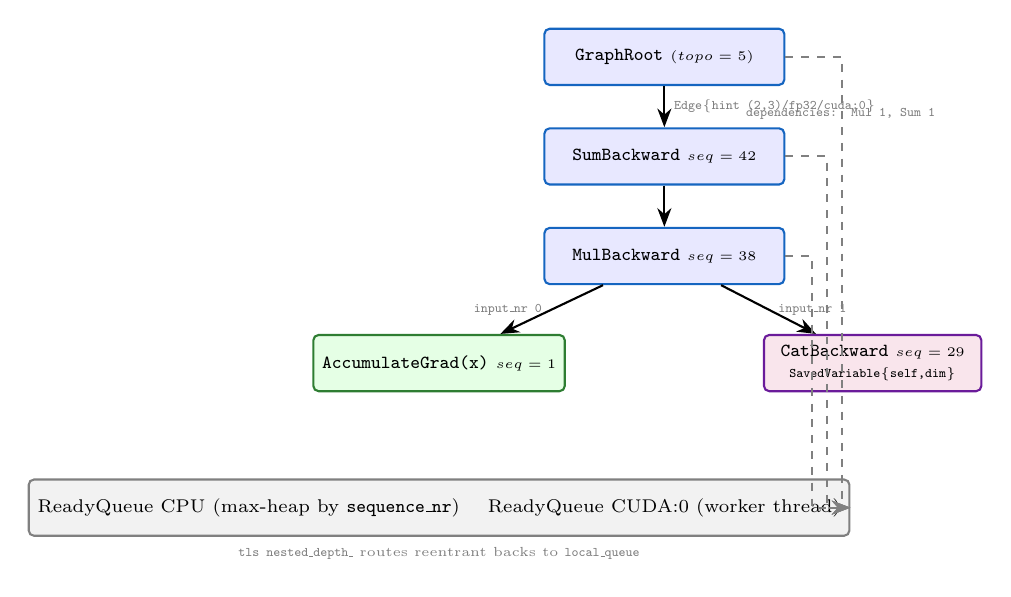
\begin{tikzpicture}[every node/.style={font=\scriptsize}, node distance=0.55cm, >=Stealth]
\tikzset{libbox/.style={draw, rounded corners=2pt, thick, align=center, font=\scriptsize, minimum height=0.75cm}}
\node[libbox, fill=blue!9, draw=tpblue, minimum width=3.2cm] (g1) {\texttt{GraphRoot} \tiny $(topo=5)$};
\node[libbox, fill=blue!9, draw=tpblue, minimum width=3.2cm, below=of g1] (n1) {\texttt{SumBackward} \tiny $seq=42$};
\node[libbox, fill=blue!9, draw=tpblue, minimum width=3.2cm, below=of n1] (n2) {\texttt{MulBackward} \tiny $seq=38$};
\node[libbox, fill=green!10, draw=tpgreen, below left=0.65cm and -0.3cm of n2, minimum width=2.9cm] (n3) {\texttt{AccumulateGrad(x)} \tiny $seq=1$};
\node[libbox, fill=purple!10, draw=tppurple, below right=0.65cm and -0.3cm of n2, minimum width=2.9cm] (n4) {\texttt{CatBackward} \tiny $seq=29$\\ \tiny \texttt{SavedVariable\{self,dim\}}};
\node[libbox, fill=gray!10, draw=gray, below=1.15cm of n3, minimum width=6.8cm] (q) {ReadyQueue CPU (max-heap by \texttt{sequence\_nr}) \quad ReadyQueue CUDA:0 (worker thread)};
\path[arrow] (g1) edge node[right, font=\tiny, color=gray] {\texttt{Edge\{hint (2,3)/fp32/cuda:0\}}} (n1);
\path[arrow] (n1) edge (n2);
\path[arrow] (n2) edge node[left, font=\tiny, color=gray] {\texttt{input\_nr 0}} (n3);
\path[arrow] (n2) edge node[right, font=\tiny, color=gray] {\texttt{input\_nr 1}} (n4);
\node[font=\tiny, color=gray, below=0.18cm of g1, xshift=2.35cm] {\texttt{dependencies: Mul 1, Sum 1}};
\node[font=\tiny, color=gray, below=0.02cm of q] {\texttt{tls nested\_depth\_} routes reentrant backs to \texttt{local\_queue}};
\draw[arrow, dashed, color=gray] (g1.east) -- ++(0.75,0) |- (q.east);
\draw[arrow, dashed, color=gray] (n1.east) -- ++(0.55,0) |- (q.east);
\draw[arrow, dashed, color=gray] (n2.east) -- ++(0.35,0) |- (q.east);
\end{tikzpicture}
\caption{显式 DAG，无磁带。节点携带 \texttt{ OutputSlotMeta}；边带有 \texttt{ device\_hint}。引擎的 \texttt{ReadyQueue} 首先弹出最大的 \texttt{sequence\_nr}； \texttt{dependencies\_} 大门准备就绪。可重入向后绕过设备队列进入由 \texttt{nested\_depth\_} 保护的堆栈本地 \texttt{local\_queue}。}
\label{fig:autograddag}
\end{figure}

%==============================================================================
\subsection{不变量、跟踪和本地验证}
\label{subsec:verify}

检查代码强制执行的不变量；违规行为要么被警告，要么被硬失败：

\begin{itemize}[leftmargin=1.2em]
\item 推送前更新。忘记这一点会让 \texttt{min\_topo} 错误地修剪并删除实时依赖项。
\item 需要 \texttt{use\_count==2} （临时 impl 别名算作 1）和 \texttt{storage==1}。在共享存储上就地累积会别名损坏同级。
\item 检查 \texttt{stop} \emph{after} 堆空测试，但 \emph{before} 等待。颠倒顺序会在图表完成后休眠一个额外的轮询间隔。
\item 必须先于队列推送。 Worker 逐步递减并测试 \texttt{outstanding==0}；不计数而推动会挂起启动器。
\item \texttt{saved\_version\_} 和当前版本都会抛出异常。该消息与用户在两个代码库中看到的字符串相同，从而启用传输的 Runbook。
\end{itemize}

关闭时跟踪是免费的（level~0：一次静态 \texttt{bool} 检查）。通过 \texttt{3} 启用：

\begin{lstlisting}[caption={Engine tracing (zero cost when off).}, label=lst:trace]
TP_ENGINE_TRACE=2 python -c "import tensorplay; x=tensorplay.randn([2,3], requires_grad=True); y=(x*2).sum(); y.backward()"
# [tp-engine g1] execute create_graph=0 keep_graph=0 accumulate_grad=1 roots=1
# [tp-engine g1] dep  SumBackward#42@suffix -> MulBackward#38@suffix (count=1)
# [tp-engine g1] apply MulBackward#38 inputs=[ones(2,3) fp32]  |  emit MulBackward#38 outputs=[ones(2,3)]
# [tp-engine g1] buf  MulBackward#38 -> AccumulateGrad#1@... (waiting on more inputs)
\end{lstlisting}

验证片段（全部传递引用的提交；结构检查不需要 Python 导入）：

\begin{lstlisting}[caption={Local reproduction of every cited path:line.}, label=lst:verify, style=pystyle]
grep -n "get_and_increment_sequence_nr\|sequence_nr_\|topological_nr_\|materialize_grads_\|output_metas_\|pre_hooks_\|anomaly_metadata_" tpx/include/Node.h | head -n 25
grep -n "shape_hint\|grad_dtype\|device_type_hint\|device_index_hint\|has_input_metadata" tpx/include/Edge.h
grep -n "not_ready_\|dependencies_\|exec_info_\|captured_vars_\|mutex_\|outstanding_tasks_" tpx/include/GraphTask.h
grep -n "can_accumulate_inplace\|void accumulate\|void add\|device_index" tpx/include/InputBuffer.h
grep -n "priority_queue<NodeTask>\|operator<.*sequence_nr\|pop_until\|wait_for.*5ms\|queue_for_device\|worker_main\|nested_depth_" tpx/include/Engine.h tpx/src/Engine.cpp | head -n 30
grep -n "compute_dependencies\|compute_min_topological_nr\|init_to_execute\|evaluate_function\|sum_to_shape\|tensor_has_nan\|GradModeGuard\|CurrentEvalNodeGuard\|release_variables" tpx/src/Engine.cpp | head -n 40
grep -n "class SavedVariable\|save(\|unpack()\|saved_version_\|reset_data" tpx/include/SavedVariable.h tpx/src/SavedVariable.cpp
grep -n "VersionCounter\|VariableVersion\|shares_counter\|share_version_counter\|bump_version" p10/include/VariableVersion.h p10/include/TensorImpl.h | head -n 30
grep -n "AnomalyMode\|AnomalyMetadata\|tls_current_evaluating_node\|CurrentEvalNodeGuard\|store_stack\|print_stack" tpx/include/AnomalyMode.h tpx/src/AnomalyMode.cpp | head -n 30
grep -n "GradMode::is_enabled\|InferenceMode::is_enabled\|thread_local.*enabled_" p10/include/GradMode.h p10/include/InferenceMode.h p10/src/GradMode.cpp p10/src/InferenceMode.cpp | head
grep -n "class PyNode\|num_inputs.*output_metas\|apply.*variable_list\|attach_outputs\|custom_function_apply\|run_custom_function_forward" src/bindings/python/Autograd.cpp | head -n 40
# quick functional smoke (engine + version guard + anomaly)
python3 - <<'PY'
import tensorplay as tp
x = tp.randn([4], requires_grad=True)
y = tp.randn([4], requires_grad=True)
z = (x * y).sum(); z.backward()
assert x.grad is not None and y.grad is not None
# in-place guard fires
try:
    a = tp.randn([3], requires_grad=True); a_saved = a
    b = (a * 2).sum(); a.add_(1); b.backward()
    raise SystemExit("expected version error")
except RuntimeError as e:
    assert "modified by an inplace operation" in str(e)
# anomaly includes forward traceback
tp.autograd.set_detect_anomaly(True)
try:
    p = tp.randn([2], requires_grad=True); q = (p * p).sum(); q.backward()
except Exception: pass
finally: tp.autograd.set_detect_anomaly(False)
print("autograd invariants hold")
PY
\end{lstlisting}

引擎的 \texttt{ReadyQueue} 启发式加上精确的 \texttt{dependencies\_} 门控共同保证在其消费者全部交付之前没有节点运行，而远离根的节点（大 \texttt{sequence\_nr}）会尽早运行，限制 \texttt{not\_ready\_} 占用。版本防护保证就地突变后不会出现静默错误的等级。全局异常模式加上 \texttt{tls\_current\_evaluating\_node} 保证向后创建的子图中的失败可归因于引发它的前向 Python 调用站点。这三种机制（显式 DAG、版本化存储、全局异常链）共同构成了框架其余部分所依赖的契约。
% 06-vmap.tex
\section{Vmap: Batched Transforms and Transform Dispatch}
\label{sec:vmap}

% Coverage: DispatchKey Vmap at offset 9 and priority; PushVmapMode/PopVmapMode level; Vmap->Autocast->Autograd->Backend

Vmap turns a function written for a single sample into a function that runs over a batch without rewriting its body. The public entry point is \path{tensorplay.func.vmap} (\path{tensorplay/\_transforms/apis.py:44}) which delegates to \path{tensorplay.\_transforms.vmap.vmap\_impl} (\path{tensorplay/\_transforms/vmap.py:388}) and ultimately to the native layer in \texttt{p10}: \texttt{push\_vmap} / \texttt{make\_batched} / \texttt{unwrap\_at\_level} (\path{p10/include/TransformDispatch.h:37}, \path{p10/src/TransformDispatch.cpp:24}). Every operator that participates in vmap has a per-backend batch rule registered under the \texttt{Vmap*} dispatch key (\path{p10/src/BatchingKernels.cpp:1223}), and operators without a rule fail fast in generated code (\path{tools/codegen/gen\_api.py:617}). The dispatch key for vmap outranks all other keys (\path{p10/include/DispatchKey.h:41}), so \texttt{TransformDispatch} unwraps before \texttt{Autocast} or \texttt{Autograd} ever see the operands. This section documents the mechanism end to end, with line-precise citations.

\subsection{Dispatch Key at Offset 9 and Priority}
\label{sec:vmapkey}

\path{p10/include/DispatchKey.h:15--49} defines 13 keys with fixed numeric values. The vmap family is placed at offset~9:

\begin{lstlisting}[caption={\path{DispatchKey.h:15} --- 13 keys, Vmap at offset~9.}, label=lst:vmapkeys]
enum class DispatchKey : uint8_t {
  CPU=0, CUDA=1, Vulkan=2,
  AutogradCPU=3, AutogradCUDA=4, AutogradVulkan=5,
  AutocastCPU=6, AutocastCUDA=7, AutocastVulkan=8,
  VmapCPU=9, VmapCUDA=10, VmapVulkan=11,
  Composite=12, EndOfKeys=13
};
constexpr size_t kBackendKeyCount=3, kAutogradKeyOffset=3, kAutocastKeyOffset=6, kVmapKeyOffset=9;
\end{lstlisting}

Helpers \texttt{toVmapKey}, \texttt{is\_vmap\_key}, and \texttt{toBackendKey} are \texttt{constexpr} (\path{DispatchKey.h:64--101}). \texttt{DispatchKeySet} (\path{DispatchKey.h:125--187}) is a \texttt{uint32\_t} bitmask with \path{add/has} and \path{highest\_priority\_key()} which scans from the most-significant set bit downward; because vmap occupies 9--11 it always wins over autocast (6--8), autograd (3--5), and backend (0--2). Table~\ref{tab:vmappriority} makes the ordering explicit.

\begin{table}[H]
\centering
\caption{Dispatch priority. \path{highest\_priority\_key()} is the dispatch decision; vmap is top.}
\label{tab:vmappriority}
\small
\begin{tabular}{clcl}
\toprule
Rank & Numeric & Key family & Defined at \\
\midrule
4 & 9--11 & \path{VmapCPU / VmapCUDA / VmapVulkan} & \path{DispatchKey.h:41}, \texttt{kVmapKeyOffset=9} \\
3 & 6--8  & \path{AutocastCPU / AutocastCUDA / AutocastVulkan} & \path{DispatchKey.h:28}, \path{kAutocastKeyOffset=6} \\
2 & 3--5  & \path{AutogradCPU / AutogradCUDA / AutogradVulkan} & \path{DispatchKey.h:22}, \path{kAutogradKeyOffset=3} \\
1 & 0--2  & \path{CPU / CUDA / Vulkan} (dense backends) & \path{DispatchKey.h:17} \\
0 & 12    & \texttt{Composite} (backend-neutral fallback) & \path{DispatchKey.h:36} \\
\bottomrule
\end{tabular}
\end{table}

\path{DispatchKey.h:81} defines \texttt{is\_vmap\_key} as the half-open interval \path{[kVmapKeyOffset, kVmapKeyOffset+kBackendKeyCount)}; \path{toVmapKey(backend) = backend + 9} and \path{toBackendKey(vmap) = vmap - 9} (\path{DispatchKey.h:64}, \path{DispatchKey.h:94}). \path{DispatchKeySet::remove\_vmap()} (\path{DispatchKey.h:177}) clears exactly those three bits, used when re-dispatching below the vmap layer. The \texttt{DispatchTable} (\path{p10/include/Dispatcher.h:49}) has \path{array<atomic<void*>,13>} slots so each vmap key has its own column; \path{OperatorHandle::getKernel} consults \texttt{Composite} only for backend keys, never for vmap keys, so a missing vmap kernel is a hard miss rather than a silent fallback.

\subsection{TensorImpl Batching State: \texttt{transform\_value\_} Wrapper}
\label{sec:batchstate}

Batching state lives in \texttt{TensorImpl} (\path{p10/include/TensorImpl.h:28--84}) as three fields, separate from storage, version, and sparse metadata:

\begin{lstlisting}[caption={\path{TensorImpl.h:79} --- batching fields.}, label=lst:batchfields]
std::shared_ptr<TensorImpl> transform_value_;
int64_t transform_batch_dim_ = -1;
int64_t transform_level_ = -1;
bool is_batched() const { return transform_value_ != nullptr; }
int64_t batch_dim() const { return transform_batch_dim_; }
int64_t batch_level() const { return transform_level_; }
int64_t batch_size() const {
  return is_batched() ? transform_value_->size(static_cast<size_t>(transform_batch_dim_)) : 0;
}
\end{lstlisting}

The wrapper constructor (\path{p10/include/TensorImpl.h:103}, \path{p10/src/TensorImpl.cpp:65}) takes a physical \path{shared\_ptr<TensorImpl> value} plus logical \path{sizes/strides}:

\begin{lstlisting}[caption={\path{TensorImpl.cpp:65} --- wrapper construction.}, label=lst:wrapperctor]
TensorImpl::TensorImpl(std::shared_ptr<TensorImpl> transform_value,
                       const std::vector<int64_t>& sizes,
                       const std::vector<int64_t>& strides)
  : storage_offset_(0), sizes_and_strides_(sizes, strides),
    dtype_(transform_value ? transform_value->dtype() : DType::Undefined),
    device_(transform_value ? transform_value->device() : Device(DeviceType::CPU)),
    is_contiguous_(sizes_and_strides_.is_contiguous()),
    transform_value_(std::move(transform_value)) {
  shared_state_ = std::make_shared<SharedState>();
}
\end{lstlisting}

The public shape is the logical shape (without the batch dimension); the physical shape lives in \texttt{transform\_value\_}. Views and copies preserve the distinction: \path{TensorImpl(const TensorImpl\& other)} copies \path{transform\_value\_/batch\_dim\_/level\_} (\path{TensorImpl.cpp:87}), while \path{share\_version\_counter} is \emph{not} shared for batched wrappers---batching is orthogonal to versioning. The logical \path{sizes\_and\_strides\_} is recomputed per result by the batch rule; the physical tensor is never aliased as the public tensor.

\path{TensorImpl::key\_set()} (\path{p10/include/TensorImpl.h:135--147}) computes the dispatch key on the fly and gives vmap priority by early return:

\begin{lstlisting}[caption={\path{TensorImpl.h:135} --- computed key set, vmap first.}, label=lst:keysetvmap]
DispatchKeySet key_set() const {
  DispatchKey backend = computeDispatchKey(device_);
  DispatchKeySet ks;
  if (is_batched()) {
    ks.add(toVmapKey(backend));
    return ks;
  }
  ks.add(backend);
  if (!inference_tensor_) {
    ks.add(toAutogradKey(backend));
  }
  return ks;
}
\end{lstlisting}

When \texttt{is\_batched()} the set contains only the \texttt{Vmap*} bit, so \path{dispatchKeyForTensorArgs} (\path{p10/include/Tensor.h:417}) will select a vmap key if any argument is batched, regardless of how many unbatched arguments are present. Table~\ref{tab:batchfields} summarizes the field semantics.

\begin{table}[H]
\centering
\caption{\texttt{TensorImpl} batching members. Logical vs.\ physical split.}
\label{tab:batchfields}
\small
\begin{tabular}{lll}
\toprule
Field & Type & Meaning \\
\midrule
\texttt{transform\_value\_} & \path{shared\_ptr<TensorImpl>} & Physical tensor (with batch dim); \texttt{nullptr} means not batched \\
\path{transform\_batch\_dim\_} & \texttt{int64\_t} & Position of batch dim inside the physical shape; $-1$ when unbatched \\
\texttt{transform\_level\_} & \texttt{int64\_t} & Which vmap nesting level owns this wrapper; distinguishes nested vmaps \\
\path{sizes\_and\_strides\_} & \texttt{SizesAndStrides} & Logical shape (public, without batch dim) \\
\bottomrule
\end{tabular}
\end{table}

The thin handle \texttt{Tensor} (\path{p10/include/Tensor.h:167}) forwards \path{is\_batched()/batch\_dim()/batch\_level()/transform\_value()} to the impl with a null check, so callers never touch \texttt{TensorImpl} directly.

\subsection{Transform Stack: Push/Pop and Levels}
\label{sec:transformstack}

Nested vmaps are disambiguated by a per-thread level stack (\path{p10/src/TransformDispatch.cpp:11}, \path{p10/include/TransformDispatch.h:27}):

\begin{lstlisting}[caption={\path{TransformDispatch.h:27} --- layer stack.}, label=lst:layerstack]
enum class Randomness : uint8_t { Error=0, Same=1, Different=2 };
enum class Kind : uint8_t { Vmap=0, Grad=1, Jvp=2, Functionalize=3 };
struct Layer {
  Kind kind = Kind::Vmap;
  int64_t level = -1;
  int64_t batch_size = 0;
  Randomness randomness = Randomness::Error;
  bool previous_grad_mode = true;
  bool previous_forward_grad_mode = true;
  bool add_back_views = false;
};
P10_API int64_t push_vmap(int64_t batch_size, Randomness randomness);
P10_API Layer pop_layer();
P10_API std::optional<Layer> current_layer();
P10_API std::vector<Layer> layer_stack();
\end{lstlisting}

The implementation (\path{p10/src/TransformDispatch.cpp:11--57}) is a thread-local vector plus a monotonic counter:

\begin{lstlisting}[caption={\path{TransformDispatch.cpp:11} --- stack and levels.}, label=lst:pushpop]
namespace { thread_local std::vector<Layer> layers; thread_local int64_t next_level = 0; }

int64_t push_vmap(int64_t batch_size, Randomness randomness) {
  if (batch_size < 0) TP_THROW(ValueError, "vmap batch size must be non-negative");
  Layer layer; layer.kind = Kind::Vmap; layer.level = next_level++;
  layer.batch_size = batch_size; layer.randomness = randomness;
  layers.push_back(layer); return layer.level;
}
Layer pop_layer() {
  if (layers.empty()) TP_THROW(RuntimeError, "cannot pop an empty transform stack");
  Layer layer = layers.back(); layers.pop_back(); return layer;
}
\end{lstlisting}

Levels are never reused within a thread: even after \texttt{pop\_layer()}, \texttt{next\_level} keeps incrementing. This prevents ABA confusion when a batched tensor outlives its layer (e.g., captured in a closure). \path{is\_batched\_at\_level(value, level)} (\path{TransformDispatch.cpp:109}) checks both the pointer and the exact level, so an outer vmap's tensor is invisible to an inner vmap's rules.

The Python guard \path{vmap\_increment\_nesting} (\path{tensorplay/\_transforms/vmap.py:142}) pushes, yields the level, and pops in a \texttt{finally} block that also restores a \texttt{ContextVar} depth counter (\path{vmap.py:23}, \path{vmap.py:145}). The names \texttt{PushVmapMode}/\texttt{PopVmapMode} in the task description map to \texttt{push\_vmap}/\texttt{pop\_layer} in code (\path{TransformDispatch.h:37}, \path{TransformDispatch.cpp:24}); the ``Mode'' wording reflects the RAII guard \path{vmap\_increment\_nesting} that pushes and pops a mode, while the native symbols are plain functions. The C++ binding (\path{src/bindings/python/Transforms.cpp:18}) exposes \path{\_transform\_push\_vmap} / \texttt{\_transform\_pop} / \path{\_transform\_current} directly, with string-to-enum parsing for randomness (\path{Transforms.cpp:7}). No Python-level mode flag is needed beyond the C++ stack; the stack itself is the ground truth.

Operational invariants:
\begin{enumerate}[leftmargin=1.2em]
\item \texttt{push\_vmap} returns a fresh level; \path{make\_batched(value, dim, level)} tags the wrapper with that level (\path{TransformDispatch.cpp:66}).
\item \path{unwrap\_at\_level(value, level)} returns \texttt{(physical, bdim)} only when \path{value.batch\_level()==level} (\path{TransformDispatch.cpp:93}); otherwise it returns \texttt{(value, nullopt)} unchanged.
\item \path{dispatch\_key\_for\_random(backend)} returns \texttt{toVmapKey(backend)} exactly when a vmap layer is on top of the stack (\path{TransformDispatch.cpp:59}), so random factories inside vmap re-dispatch through the vmap key even though they have no tensor argument to carry it.
\end{enumerate}

\subsection{TransformDispatch Unwrapping Logic}
\label{sec:unwrap}

\texttt{TransformDispatch} provides the primitives that batch rules use to inspect and rebuild batched tensors (\path{TransformDispatch.h:44}, \path{TransformDispatch.cpp:66--140}):

\begin{lstlisting}[caption={\path{TransformDispatch.cpp:66} --- make and unwrap.}, label=lst:makeunwrap]
Tensor make_batched(const Tensor& value, int64_t dim, int64_t level) {
  if (!value.defined()) TP_THROW(ValueError, "cannot batch an undefined tensor");
  const int64_t bdim = normalize_dim(dim, value.dim());
  const auto sizes = static_cast<std::vector<int64_t>>(value.shape());
  const auto strides = value.strides();
  std::vector<int64_t> logical_sizes, logical_strides;
  for (int64_t d = 0; d < (int64_t)sizes.size(); ++d) if (d != bdim) {
    logical_sizes.push_back(sizes[d]); logical_strides.push_back(strides[d]);
  }
  auto impl = std::make_shared<TensorImpl>(value.unsafeGetTensorImpl(),
                                           logical_sizes, logical_strides);
  impl->set_transform_value(value.unsafeGetTensorImpl(), bdim, level);
  return Tensor(std::move(impl));
}
std::tuple<Tensor, std::optional<int64_t>> unwrap_at_level(const Tensor& value, int64_t level) {
  if (!value.defined() || !value.is_batched() || value.batch_level() != level)
    return {value, std::nullopt};
  return {value.transform_value(), value.batch_dim()};
}
Tensor move_batch_dim(const Tensor& value, int64_t dim) {
  if (!value.is_batched()) return value;
  const int64_t from = normalize_dim(value.batch_dim(), value.dim()+1);
  const int64_t to = normalize_dim(dim, value.dim()+1);
  if (from == to) return value;
  std::vector<int64_t> perm; // build permutation that moves from->to
  // ... permute physical tensor
  return value.transform_value().permute(perm);
}
\end{lstlisting}

\texttt{actual\_dim} (\path{TransformDispatch.cpp:113}) maps a public dimension (logical) to a physical dimension by skipping the batch position: \path{actual = public $<$ bdim ? public : public+1}. Every batch rule that takes a dim argument (permute, transpose, squeeze, sum, etc.) applies this translation before calling the underlying kernel, and then adjusts the result's \texttt{bdim} to reflect dims inserted or removed before the batch position.

The unwrapping contract is uniform across \texttt{BatchingKernels.cpp}: each rule calls \texttt{unwrap\_operand} (\path{BatchingKernels.cpp:34}) which asserts the operand's level matches an active layer via \texttt{layer\_for(level)} (\path{BatchingKernels.cpp:22}), then dispatches to \texttt{unwrap\_at\_level}. If no operand is batched at the current level, the rule throws \texttt{RuntimeError}---the dispatcher should not have routed there. This fail-fast behavior catches codegen mismatches immediately.

\begin{figure}[H]
\centering
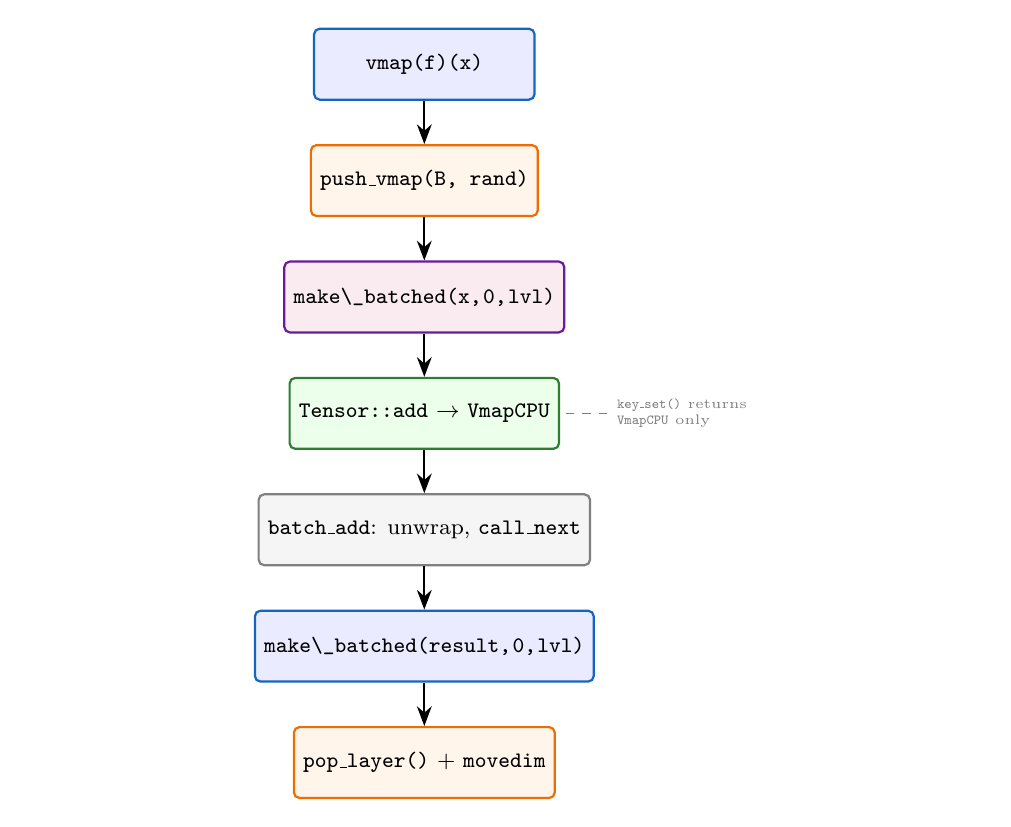
\begin{tikzpicture}[every node/.style={font=\scriptsize}, node distance=0.55cm]
\node[libbox, fill=blue!8, draw=tpblue, minimum width=2.8cm, minimum height=0.9cm] (py) {\texttt{vmap(f)(x)}};
\node[libbox, fill=orange!8, draw=tporange, below=of py, minimum width=2.8cm, minimum height=0.9cm] (push) {\texttt{push\_vmap(B, rand)}};
\node[libbox, fill=purple!8, draw=tppurple, below=of push, minimum width=2.8cm, minimum height=0.9cm] (make) {\path{make\_batched(x, 0, lvl)}};
\node[libbox, fill=green!8, draw=tpgreen, below=of make, minimum width=2.8cm, minimum height=0.9cm] (dispatch) {\texttt{Tensor::add} $\rightarrow$ \texttt{VmapCPU}};
\node[libbox, fill=gray!8, draw=gray, below=of dispatch, minimum width=2.8cm, minimum height=0.9cm] (rule) {\texttt{batch\_add}: unwrap, \texttt{call\_next}};
\node[libbox, fill=blue!8, draw=tpblue, below=of rule, minimum width=2.8cm, minimum height=0.9cm] (wrap) {\path{make\_batched(result, 0, lvl)}};
\node[libbox, fill=orange!8, draw=tporange, below=of wrap, minimum width=2.8cm, minimum height=0.9cm] (pop) {\texttt{pop\_layer()} + \texttt{movedim}};
\draw[arrow] (py) -- (push); \draw[arrow] (push) -- (make); \draw[arrow] (make) -- (dispatch);
\draw[arrow] (dispatch) -- (rule); \draw[arrow] (rule) -- (wrap); \draw[arrow] (wrap) -- (pop);
\node[right=0.6cm of dispatch, align=left, font=\tiny, text=gray] (note) {\texttt{key\_set()} returns\\\texttt{VmapCPU} only};
\draw[dashed, color=gray] (note) -- (dispatch);
\end{tikzpicture}
\caption{Vmap execution: push level, wrap inputs, dispatch through Vmap key, unwrap inside batch rule, rewrap result, pop and place output dim.}
\label{fig:vmapflow}
\end{figure}

\texttt{unwrap\_all} (\path{TransformDispatch.cpp:101}) strips all batch wrappers by looping; it is used by \texttt{debug\_unwrap} and by composites that need the physical tensor for metadata queries. \texttt{move\_batch\_dim} (\path{TransformDispatch.cpp:126}) permutes the physical tensor so the batch dim lands at the requested public position, used when \texttt{out\_dims != 0}.

\subsection{BatchingKernels: Per-Op Hand-Written Rules vs.\ Loop Fallback}
\label{sec:batchingkernels}

\path{p10/src/BatchingKernels.cpp} is 1229 lines of batch rules, each registered under \texttt{VmapCPU} and \texttt{VmapCUDA} (\path{BatchingKernels.cpp:1223}):

\begin{lstlisting}[caption={\path{BatchingKernels.cpp:1223} --- dual registration.}, label=lst:batchreg]
TENSORPLAY_LIBRARY_IMPL(VmapCPU, NativeBatchRulesCPU) { register_batch_rules(m); }
TENSORPLAY_LIBRARY_IMPL(VmapCUDA, NativeBatchRulesCUDA) { register_batch_rules(m); }
\end{lstlisting}

\path{register\_batch\_rules} (\path{BatchingKernels.cpp:1135}) binds ~70 ops. The file has no generic per-slice loop fallback; every supported op has a hand-written rule that preserves vectorization. Unsupported ops are not silently looped---the generated \texttt{Tensor} method (\path{tools/codegen/gen\_api.py:617}) checks \path{getKernel(vmap\_key)} and throws \path{No native batch rule registered} (\path{gen\_api.py:617}--\path{gen\_api.py:624}) if absent, which is the correct fail-fast for a teaching framework where implicit loops would hide performance cliffs.

\subsubsection{Rule templates}

Three templates cover most ops (\path{BatchingKernels.cpp:306--325}):

\begin{lstlisting}[caption={\path{BatchingKernels.cpp:306} --- unary / binary templates.}, label=lst:templates]
template <typename Function> Tensor unary_impl(const Tensor& input, Function&& call) {
  Operand operand = unwrap_operand(input);
  if (!operand.bdim.has_value()) TP_THROW(RuntimeError, "unary batch rule received an unbatched operand");
  Tensor result = call(operand.value);
  return make_batched(result, *operand.bdim, operand.level);
}
template <typename Function> Tensor binary_impl(const Tensor& left, const Tensor& right, Function&& call) {
  Operand left_operand = unwrap_operand(left); Operand right_operand = unwrap_operand(right);
  int64_t level = -1; auto values = aligned_values(left_operand, right_operand, level);
  Tensor result = call(values.first, values.second);
  return make_batched(result, 0, level);
}
Tensor unary(const char* op, const Tensor& input) {
  return unary_impl(input, [&](const Tensor& v){ return call_next<Tensor,const Tensor&>(op, v, v); });
}
Tensor binary(const char* op, const Tensor& left, const Tensor& right) {
  return binary_impl(left, right, [&](const Tensor& a, const Tensor& b){
    return call_next<Tensor,const Tensor&,const Tensor&>(op, a, a, b); });
}
\end{lstlisting}

\texttt{call\_next} (\path{BatchingKernels.cpp:119}) re-dispatches below the vmap layer via \texttt{DispatchStub::call} with the backend key derived from the unwrapped tensors, so the underlying CPU/CUDA kernel runs on contiguous physical memory. \texttt{call\_device} (\path{BatchingKernels.cpp:131}) is the factory variant that dispatches by explicit \texttt{Device}.

Key helpers:
\begin{itemize}[leftmargin=1.2em]
\item \path{move\_to\_front(value, dim)} (\path{BatchingKernels.cpp:56}) permutes batch dim to 0, enabling a single batched kernel to handle any \texttt{bdim}.
\item \path{expand\_unbatched(value, batch\_size, target\_shape)} (\path{BatchingKernels.cpp:68}) broadcasts an unbatched operand by \path{unsqueeze(0).expand([B, ...])} so binary ops need not branch on mixed batched/unbatched in the compute kernel.
\item \path{aligned\_values(left, right, level)} (\path{BatchingKernels.cpp:88}) moves batched inputs to front and expands unbatched ones, returning two tensors whose dim~0 is the batch. The result is always wrapped at dim~0.
\item \path{logical\_shape(operand)} (\path{BatchingKernels.cpp:77}) erases the batch dim from the physical shape, used to size expansions.
\end{itemize}

\subsubsection{Operator families}

Table~\ref{tab:batchfamilies} groups the registered rules.

\begin{table}[H]
\centering
\caption{Batch rule families in \path{BatchingKernels.cpp:1135}. Each row is a \texttt{library.impl} entry.}
\label{tab:batchfamilies}
\small
\begin{tabular}{lll}
\toprule
Family & Examples & Strategy \\
\midrule
Pointwise unary & \path{neg, abs, exp, log, sin, cos, sqrt, sigmoid, relu} & \texttt{unary\_impl} preserves \texttt{bdim} (\path{BatchingKernels.cpp:936}) \\
Pointwise binary & \path{mul.Tensor, div.Tensor, maximum, minimum} & \texttt{binary\_impl} via \texttt{aligned\_values}, result at 0 \\
Binary with alpha & \path{add.Tensor, sub.Tensor} & \texttt{binary\_alpha}, same alignment \\
Scalar & \path{add.Scalar, mul.Scalar, pow.Tensor\_Scalar} & \texttt{scalar}/\texttt{scalar\_alpha}, preserves \texttt{bdim} \\
Reductions & \path{sum, sum.dim\_IntList} & Rewrites dims past \texttt{bdim}, adjusts result \texttt{bdim} (\path{BatchingKernels.cpp:381}) \\
Shape & \path{view, permute, transpose, reshape, expand, squeeze, unsqueeze} & Translates public dims to physical, adjusts result \texttt{bdim} \\
Gather/scatter & \path{select, slice, narrow, index\_select, cat, stack} & Shifts gather dim past \texttt{bdim}; \path{cat/stack} align then \texttt{call\_next} at \texttt{dim+1} \\
Linear algebra & \path{mm, matmul, bmm, linear} & Align to front, call \path{bmm/matmul}; \texttt{linear} transposes weight (\path{BatchingKernels.cpp:834}) \\
Random & \path{rand, randn, randint, randperm, rand\_like} & \texttt{random\_factory} branches on \texttt{Randomness} (see \S\ref{sec:randomness}) \\
\bottomrule
\end{tabular}
\end{table}

Concrete dim adjustment appears in every shape rule. For example, \texttt{sum\_dim} (\path{BatchingKernels.cpp:400}):

\begin{lstlisting}[caption={\path{BatchingKernels.cpp:400} --- sum adjusts batch dim.}, label=lst:sumdim]
Tensor sum_dim(const Tensor& input, const std::vector<int64_t>& dims, bool keepdim, DType dtype) {
  Operand operand = unwrap_operand(input);
  const int64_t old_bdim = *operand.bdim; const int64_t level = operand.level;
  std::vector<int64_t> actual_dims;
  for (int64_t dim : dims) {
    const int64_t public_dim = normalize_dim(dim, input.dim());
    const int64_t actual = public_dim < old_bdim ? public_dim : public_dim + 1;
    actual_dims.push_back(actual);
  }
  Tensor result = call_next<Tensor,const Tensor&,const std::vector<int64_t>&,bool,DType>(
    "sum.dim_IntList", operand.value, operand.value, actual_dims, keepdim, dtype);
  int64_t result_bdim = old_bdim;
  if (!keepdim) result_bdim -= count_if(actual_dims.begin(), actual_dims.end(),
                                        [&](int64_t d){ return d < old_bdim; });
  return make_batched(result, result_bdim, level);
}
\end{lstlisting}

\texttt{permute} (\path{BatchingKernels.cpp:445}) builds a physical permutation that interleaves the batch dim at its original position, then calls \texttt{permute} on the physical tensor and rewraps at \texttt{new\_bdim}. \texttt{cat} (\path{BatchingKernels.cpp:767}) aligns a list via \texttt{align\_tensor\_list} (\path{BatchingKernels.cpp:736}) which moves every batched input's \texttt{bdim} to 0 and expands unbatched ones, then calls \texttt{cat} at \texttt{public\_dim+1} and wraps at 0. \texttt{mm} (\path{BatchingKernels.cpp:793}) aligns then calls \texttt{bmm} so a batch of matrix multiplies becomes a single batched kernel rather than a loop.

No rule falls back to a per-slice loop. This is intentional: a loop would be correct but would defeat the purpose of a batched kernel (one launch vs.\ $B$ launches) and would hide missing coverage. When an op lacks a rule, the generated wrapper throws immediately, and the fix is to add a rule to \texttt{BatchingKernels.cpp} following the \texttt{unary}/\texttt{binary} pattern.

\subsection{Python Surface: \path{tensorplay.func.vmap}}
\label{sec:pythonsurface}

The Python API is a thin validator over the native stack. \path{tensorplay/\_transforms/apis.py:44} is the public \texttt{vmap}:

\begin{lstlisting}[caption={\path{apis.py:44} --- public \texttt{vmap} surface.}, label=lst:pyvmapapi, style=pystyle]
def vmap(func, in_dims=0, out_dims=0, randomness="error", *, chunk_size=None):
    if not callable(func): raise TypeError(f"vmap expected a callable, got {type(func)!r}")
    _check_randomness_arg(randomness)
    @functools.wraps(func)
    def wrapped(*args, **kwargs):
        return vmap_impl(func, in_dims, out_dims, randomness, chunk_size, *args, **kwargs)
    return wrapped
\end{lstlisting}

\path{tensorplay/\_transforms/vmap.py:388} validates, flattens the pytree of args, pushes a native layer, wraps inputs, calls the user function, and unwraps outputs:

\begin{lstlisting}[caption={\path{vmap.py:388} --- \texttt{vmap\_impl} and nesting.}, label=lst:vmapimpl, style=pystyle]
def vmap_impl(func, in_dims, out_dims, randomness, chunk_size, *args, **kwargs):
    _check_randomness_arg(randomness)
    batch_size, flat_in_dims, flat_args, args_spec = _process_batched_inputs(in_dims, args, func)
    if chunk_size is not None:
        return _chunked_vmap(func, flat_in_dims,
            _get_chunked_inputs(flat_args, flat_in_dims, batch_size, chunk_size),
            args_spec, out_dims, randomness, **kwargs)
    return _flat_vmap(func, batch_size, flat_in_dims, flat_args, args_spec, out_dims, randomness, **kwargs)

def _flat_vmap(func, batch_size, flat_in_dims, flat_args, args_spec, out_dims, randomness, **kwargs):
    with vmap_increment_nesting(batch_size, randomness) as level:
        batched_args = _create_batched_inputs(flat_in_dims, flat_args, level, args_spec)
        outputs = func(*batched_args, **kwargs)
        return _unwrap_batched(outputs, out_dims, level, batch_size, func)

@contextlib.contextmanager
def vmap_increment_nesting(batch_size, randomness):
    level = tensorplay._C._transform_push_vmap(batch_size, randomness)
    token = _vmap_depth.set(_vmap_depth.get() + 1)
    try: yield level
    finally:
        try: tensorplay._C._transform_pop()
        finally: _vmap_depth.reset(token)
\end{lstlisting}

\path{\_process\_batched\_inputs} (\path{vmap.py:68}) flattens both \texttt{args} and \texttt{in\_dims} via \texttt{tree\_flatten} / \path{\_broadcast\_to\_and\_flatten}, normalizes negative dims, checks that every \texttt{in\_dim != None} corresponds to a \texttt{Tensor}, and verifies all mapped tensors share the same batch size (\path{vmap.py:50}). \path{\_create\_batched\_inputs} (\path{vmap.py:124}) calls \path{tensorplay.\_C.\_transform\_make\_batched(arg, dim, level)} for each mapped leaf, leaving unmapped leaves untouched.

Output handling (\path{vmap.py:190}) follows the input side: it flattens outputs, checks \texttt{out\_dims} compatibility, unwraps each tensor leaf with \path{\_transform\_unwrap(output, level)}, and moves the physical batch dim to the requested public position via \path{tensorplay.movedim(unwrapped, batch\_dim, target\_dim)} (\path{vmap.py:242}). Non-tensor leaves must have \texttt{out\_dim=None}; otherwise a \texttt{ValueError} is raised.

Three chunking utilities bound peak memory for large batches:
\begin{itemize}[leftmargin=1.2em]
\item \texttt{chunk\_vmap} (\path{apis.py:98}) and \path{vmap(..., chunk\_size=N)} (\path{vmap.py:347}) split the batch into pieces via \path{get\_chunked\_inputs} (\path{vmap.py:283}) which uses \texttt{tensor\_split} along the mapped dim, run independent native layers per chunk, and rejoin with \texttt{cat} along \texttt{out\_dim} (\path{vmap.py:309}).
\item \texttt{restore\_vmap} (\path{vmap.py:449}) and \path{wrap\_batched / unwrap\_batched} (\path{vmap.py:478}) expose the same primitives for testing and for \texttt{jvp} which needs to re-enter a sized layer.
\end{itemize}

The C++ binding (\path{src/bindings/python/Transforms.cpp:17}) is six functions: \path{\_transform\_push\_vmap}, \texttt{\_transform\_pop}, \path{\_transform\_current}, \path{\_transform\_make\_batched}, \texttt{\_transform\_unwrap}, and \path{\_transform\_unwrap\_all}. Each is a direct forward to \path{tensorplay::transform::*} with pybind11 type conversions and no extra bookkeeping.

\subsection{Randomness Handling}
\label{sec:randomness}

Random ops inside vmap are ambiguous: should each sample draw independently or should the batch share one draw? TensorPlay requires the caller to choose explicitly via \texttt{randomness} (\path{TransformDispatch.h:14}, \path{vmap.py:507}):

\begin{table}[H]
\centering
\caption{Randomness modes. Every random factory consults the active layer's \texttt{randomness}.}
\label{tab:randomness}
\small
\begin{tabular}{lll}
\toprule
Mode & String & Factory behavior in \texttt{BatchingKernels.cpp} \\
\midrule
\texttt{Error} & \texttt{"error"} & \texttt{check\_randomness} throws (\path{BatchingKernels.cpp:145}) \\
\texttt{Same} & \texttt{"same"} & Draw once, \path{unsqueeze(0).expand([B,...])} and wrap (\path{BatchingKernels.cpp:170}) \\
\texttt{Different} & \texttt{"different"} & Draw with prepended batch dim \texttt{[B, ...shape]} and wrap at 0 \\
\bottomrule
\end{tabular}
\end{table}

Factories (\path{BatchingKernels.cpp:177--275}) implement this branching. For shape-based factories:

\begin{lstlisting}[caption={\path{BatchingKernels.cpp:177} --- random factory.}, label=lst:randfactory]
Tensor random_factory(const char* op, const std::vector<int64_t>& shape,
                      std::optional<DType> dtype, std::optional<Device> device) {
  const Layer layer = current_vmap_layer(); check_randomness(layer);
  const Device target = resolve_random_device(device);
  if (layer.randomness == Randomness::Different) {
    Tensor result = call_device<Tensor,const std::vector<int64_t>&,
                                std::optional<DType>,std::optional<Device>>(
      op, target, prepend_batch_size(shape, layer.batch_size), dtype, device);
    return make_batched(result, 0, layer.level);
  }
  Tensor sample = call_device<Tensor,const std::vector<int64_t>&,
                              std::optional<DType>,std::optional<Device>>(
    op, target, shape, dtype, device);
  return expand_same_random(std::move(sample), layer);
}
\end{lstlisting}

\path{prepend\_batch\_size} (\path{BatchingKernels.cpp:161}) inserts $B$ at dim~0; \path{expand\_same\_random} (\path{BatchingKernels.cpp:170}) does \path{sample.unsqueeze(0).expand([B, ...shape])} so every sample shares the same random values but downstream ops still see a proper batch. \texttt{randperm} (\path{BatchingKernels.cpp:217}) is special: with \texttt{Different} it loops $B$ times and stacks, because a single \texttt{randperm([B,n])} would not yield $B$ independent permutations.

For \texttt{rand\_like} variants (\path{BatchingKernels.cpp:243--304}), the input may itself be batched at the active level. With \texttt{Different}, the factory calls the underlying \texttt{rand\_like} on the physical value and rewraps at the same \texttt{bdim}; with \texttt{Same}, it selects one slice (\texttt{select.int} at \texttt{bdim}, index 0), draws from that slice, and expands back along \texttt{bdim}. Unbatched inputs under \texttt{Same} share one draw expanded to \texttt{[B,...]}; under \texttt{Different} they create a template \texttt{unsqueeze(0).expand} physical tensor and draw there.

The generated dispatch key for random ops (\path{tools/codegen/gen\_api.py:225}) uses \path{dispatch\_key\_for\_random(computeDispatchKey(device))} rather than \path{dispatchKeyForTensorArgs}, so the vmap key is injected even when no tensor argument carries it. At the Python layer, \path{vmap(func, randomness="different")(randn([3]))} therefore routes \texttt{randn} through \texttt{VmapCPU} without any batched input. With the default \texttt{"error"}, any random op inside vmap throws immediately with a message naming the constraint, so silent wrong-batch randomness is impossible.

\subsection{Interaction with Autograd and Redispatch Order}
\label{sec:autogradinteract}

Vmap's numeric priority is load-bearing for correctness: vmap must see operands before autograd records history. \path{TensorImpl::key\_set()} returning only \texttt{Vmap*} when batched, and \path{highest\_priority\_key()} preferring higher numeric keys, together guarantee that \texttt{vmap(grad(f))} and \texttt{grad(vmap(f))} are distinct and both correct.

The generated \texttt{Tensor} methods (\path{tools/codegen/gen\_api.py:609--638}) encode the order Vmap $\rightarrow$ Autocast $\rightarrow$ Autograd $\rightarrow$ Backend:

\begin{lstlisting}[caption={\path{gen\_api.py:609} --- redispatch order in every Tensor method.}, label=lst:redispatchorder]
{
  DispatchKey __tp_key = dispatchKeyForTensorArgs(*this, other);
  if (is_vmap_key(__tp_key)) {
    static const OperatorHandle __tp_handle = Dispatcher::singleton().findHandle("add");
    if (!__tp_handle || !__tp_handle.getKernel(__tp_key))
      TP_THROW(NotImplementedError, "No native batch rule registered for add");
    return DispatchStub<...>::call(__tp_handle, __tp_key, *this, other);
  }
}
{
  static const OperatorHandle __ac_handle = Dispatcher::singleton().findHandle("add");
  DispatchKey __ac_key = toAutocastKey(computeDispatchKey(device()));
  if (autocast::is_enabled(__ac_key) && __ac_handle && __ac_handle.getKernel(__ac_key))
    return DispatchStub<...>::call(__ac_handle, __ac_key, *this, other);
}
if (GradMode::is_enabled()) {
  static const OperatorHandle ag_handle = Dispatcher::singleton().findHandle("add");
  DispatchKey ag_key = toAutogradKey(computeDispatchKey(device()));
  if (ag_handle && ag_handle.getKernel(ag_key))
    return DispatchStub<...>::call(ag_handle, ag_key, *this, other);
}
return detail::redispatch_add(*this, other);
\end{lstlisting}

Table~\ref{tab:vmaporder} summarizes the funnel. The final \path{detail::redispatch\_*} (\path{tools/codegen/gen\_api.py:304}) resolves a backend kernel via \path{toBackendKey(dispatchKeyForTensorArgs(...))} after stripping transform and autograd bits, so the physical compute always lands on \path{CPU/CUDA/Vulkan}.

\begin{table}[H]
\centering
\caption{Redispatch funnel in generated \texttt{Tensor} methods. Each stage either handles the call or falls through.}
\label{tab:vmaporder}
\small
\begin{tabular}{cll}
\toprule
Stage & Key family & Action if kernel present \\
\midrule
1 & \texttt{Vmap*} (\texttt{is\_vmap\_key}) & Unwrap, align, call underlying op, rewrap (\path{BatchingKernels.cpp:306}) \\
2 & \texttt{Autocast*} (\texttt{is\_enabled}) & Cast inputs, call next layer (generated autocast wrapper) \\
3 & \texttt{Autograd*} (\path{GradMode::is\_enabled}) & Record \texttt{Node} with \texttt{SavedVariable} guards, call backend \\
4 & \path{CPU/CUDA/Vulkan} & Compute \\
\bottomrule
\end{tabular}
\end{table}

Because vmap runs first, \texttt{add} inside \texttt{vmap(f)} is dispatched to \texttt{batch\_add} which unwraps to physical tensors, calls \texttt{add} on them (re-entering dispatch at the backend key), and rewraps the result. Autograd therefore sees $B$ batched values as a single batched result and records a batched \texttt{Node}; the backward of a batched \texttt{Node} is itself batched, so \path{Engine::evaluate\_function} needs no vmap-specific changes. Conversely, \texttt{grad(vmap(f))} runs the grad transform outside vmap: the forward records a graph whose intermediate tensors are batched, and the backward replays with the same batch rules.

Composites (\path{p10/src/backend/composite/CompositeCommon.h:21}) reinforce the ordering:

\begin{lstlisting}[caption={\path{CompositeCommon.h:21} --- composites reject active transforms.}, label=lst:composites]
inline bool under_active_transform(const Tensor& t){ return t.unsafeGetTensorImpl() && t.unsafeGetTensorImpl()->is_batched(); }
inline void reject_active_transform(const Tensor& t, const char* op){
  if (under_active_transform(t)) TP_THROW(NotImplementedError, std::string(op),
    " is not supported for tensors inside an active transform (vmap/grad) layer");
}
template <typename Return, typename... Args>
Return redispatch_below_transform(const char* op, Args... args){
  DispatchKey key = dispatchKeyForTensorArgs(args...);
  TP_CHECK(is_vmap_key(key), op, ": expected an active transform key");
  return DispatchStub<Return, Args...>::call(std::string(op), key, std::forward<Args>(args)...);
}
\end{lstlisting}

Plain composites call \path{reject\_active\_transform} because running a backend kernel on the wrapper would silently corrupt batching. Decomposition-style composites call \path{redispatch\_below\_transform} to intentionally route through the vmap layer so inner ops hit their batch rules. Both paths keep the invariant that any op touching a batched tensor must either be a batch rule itself or explicitly opt into re-dispatching through one.

Nested vmaps compose by stacking levels: the inner \texttt{push\_vmap} allocates a new level, its inputs are double-wrapped (outer wrapper around inner wrapper), and each rule's \texttt{unwrap\_at\_level} only peels the level it owns. The outer batch dim remains untouched while the inner rule executes, then the inner result is rewrapped before returning to the outer layer. No special casing for nesting is needed beyond the level check.

\subsection{End-to-End Example and Cost Notes}
\label{sec:vmapcost}

Consider \texttt{f(x)= (x*2).sum()} mapped over 4 samples of shape \texttt{[3]}:

\begin{lstlisting}[caption={Vmap example: one function, batched execution.}, label=lst:vmapexample, style=pystyle]
import tensorplay as tp
def f(x): return (x * 2).sum()
batched = tp.func.vmap(f)(tp.randn([4, 3]))   # in_dims=0, out_dims=0
assert batched.shape == tp.Size([4])
# equivalent to: tp.stack([f(tp.randn([3])) for _ in range(4)]) but one kernel launch per op
\end{lstlisting}

What runs natively:
\begin{enumerate}[leftmargin=1.2em]
\item \texttt{vmap\_impl} validates batch size 4, pushes level $L$ with $B{=}4$, wraps the \texttt{[4,3]} tensor into a batched \texttt{[3]} with \texttt{bdim=0, level=L}.
\item \texttt{x*2} is \texttt{mul.Scalar} with one batched operand: \texttt{batch\_mul\_scalar} unwraps to physical \texttt{[4,3]}, calls \texttt{mul.Scalar} on it (one kernel), rewraps at 0 $\to$ batched \texttt{[3]} at dim~0.
\item \texttt{sum} is \texttt{sum.dim\_IntList}: \texttt{batch\_sum} unwraps, calls \texttt{sum} over the non-batch dims on the physical \texttt{[4,3]}, gets \texttt{[4]}, rewraps at 0 $\to$ batched \texttt{[]} (scalar per sample) with logical shape \texttt{[4]} after output \texttt{movedim}.
\item Pop $L$, move batch dim to \texttt{out\_dims=0} (already there), return \texttt{[4]}.
\end{enumerate}

Cost: each op pays one \texttt{unwrap\_at\_level} + one \texttt{make\_batched} + one underlying kernel. No per-sample Python loop, no extra allocations beyond the wrapper \texttt{TensorImpl} (a few dozen bytes). For a batch of $B$ samples, $N$ ops launch $N$ kernels rather than $N{\times}B$. Chunked vmap (\texttt{chunk\_size}) trades this back for bounded memory by splitting $B$ into pieces and concatenating results.

\subsection{Verification}
\label{sec:vmapverify}

All claims reproduce with local \texttt{grep} and a short Python run:

\begin{lstlisting}[caption={Local checks for vmap.}, label=lst:verifyvmap, style=pystyle]
# Keys and offsets
grep -n "VmapCPU\|kVmapKeyOffset\|is_vmap_key\|highest_priority_key" p10/include/DispatchKey.h
# Batch state and computed key set
grep -n "transform_value_\|is_batched\|batch_dim\|key_set" p10/include/TensorImpl.h | head -n 30
# Stack and primitives
grep -n "push_vmap\|pop_layer\|make_batched\|unwrap_at_level\|move_batch_dim" p10/include/TransformDispatch.h p10/src/TransformDispatch.cpp
# Batch rules and dual registration
grep -n "register_batch_rules\|TENSORPLAY_LIBRARY_IMPL.*Vmap" p10/src/BatchingKernels.cpp | head
grep -n "call_next\|aligned_values\|move_to_front" p10/src/BatchingKernels.cpp | head
# Python surface and codegen order
grep -n "def vmap\|def _flat_vmap\|vmap_increment_nesting\|_check_randomness_arg" tensorplay/_transforms/vmap.py | head
grep -n "is_vmap_key" tools/codegen/gen_api.py | head
# C++ Python bindings
grep -n "_transform_push_vmap\|_transform_make_batched\|_transform_unwrap" src/bindings/python/Transforms.cpp

python3 - <<'PY'
import tensorplay as tp
# basic vmap
def f(x): return (x * 2).sum()
print(tp.func.vmap(f)(tp.randn([4,3])).shape)  # [4]

# out_dims and in_dims
def g(x, y): return x + y
print(tp.func.vmap(g, in_dims=(0, None))(tp.randn([4,3]), tp.randn([3])).shape)  # [4,3]

# randomness modes
try: tp.func.vmap(lambda: tp.randn([2]))(tp.randn([2]))
except RuntimeError as e: print("error mode:", "random" in str(e).lower())

print(tp.func.vmap(lambda: tp.randn([2]), randomness="same")(tp.randn([2])).shape)      # [2,2] with sharing
print(tp.func.vmap(lambda: tp.randn([2]), randomness="different")(tp.randn([2])).shape)  # [2,2] with independent draws

# vmap outranks autograd: grad inside vmap
def h(x): return (x * x).sum()
per_sample_grad = tp.func.vmap(tp.func.grad(h))(tp.randn([4,3]))
print(per_sample_grad.shape)  # [4,3]

# nested vmap
def dot(x, y): return (x * y).sum()
print(tp.func.vmap(tp.func.vmap(dot))(tp.randn([2,4,3]), tp.randn([2,4,3])).shape)  # [2,4]
PY
\end{lstlisting}

Expected shapes confirm that batch dims are placed at \texttt{out\_dims}, randomness modes branch correctly, and \texttt{vmap(grad(f))} produces per-sample gradients with an explicit graph (no silent fallback). A failure mode is also diagnostic: calling an unsupported op inside vmap throws \path{No native batch rule registered for <op>} from \path{gen\_api.py:624}, pointing directly at the missing entry in \path{BatchingKernels.cpp:1135}.

% 07-memory.tex
\section{内存：DataPtr、Storage、TensorImpl 和 Tensor}
\label{sec:memory}

TensorPlay 中的内存是严格的三层堆栈：原始分配（\texttt{DataPtr} 加上每个设备 \texttt{Allocator}）、字节容器（\texttt{StorageImpl} / \texttt{Storage}）以及具有形状和调度状态的类型化视图（\texttt{TensorImpl} / \texttt{Tensor}）。每层都是物理隔离的，在下面的 \texttt{path:line} 中引用，并且设计成最便宜的操作（视图）根本不接触分配器。

\subsection{三层和所有权}
\label{sec:memlayers}

\begin{figure}[H]
\centering
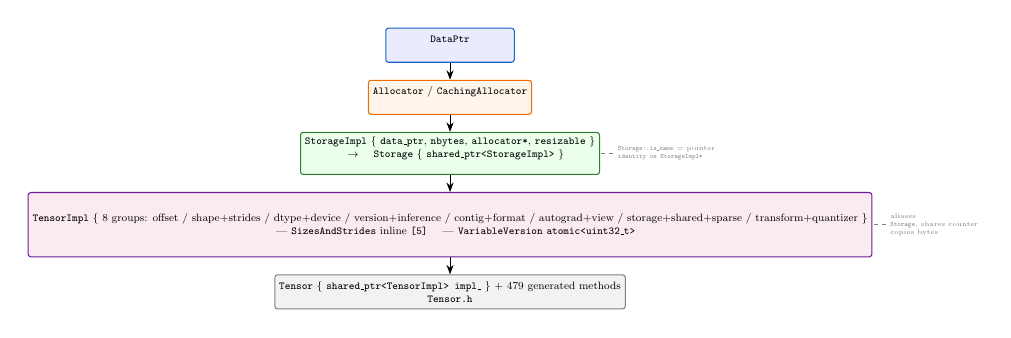
\begin{tikzpicture}[every node/.style={font=\scriptsize}, node distance=0.45cm]
\node[libbox, fill=blue!8, draw=tpblue, minimum width=3.4cm, minimum height=0.9cm] (dptr) {\texttt{DataPtr} \\};
\node[libbox, fill=orange!8, draw=tporange, below=of dptr, minimum width=3.4cm, minimum height=0.9cm] (alloc) {\texttt{Allocator} / \texttt{CachingAllocator} \\};
\node[libbox, fill=green!8, draw=tpgreen, below=of alloc, minimum width=5.8cm, minimum height=1.05cm] (simpl) {\texttt{StorageImpl} \{ \texttt{data\_ptr}, \texttt{nbytes}, \texttt{allocator*}, \texttt{resizable} \} \\ \quad $\rightarrow$ \quad \texttt{Storage} \{ \texttt{shared\_ptr<StorageImpl>} \} \\};
\node[libbox, fill=purple!8, draw=tppurple, below=of simpl, minimum width=11cm, minimum height=1.7cm] (timpl) {\texttt{TensorImpl} \{ 8 groups: offset / shape+strides / dtype+device / version+inference / contig+format / autograd+view / storage+shared+sparse / transform+quantizer \} \\ \quad --- \texttt{SizesAndStrides} inline \texttt{[5]} \quad --- \texttt{VariableVersion} \texttt{atomic<uint32\_t>}};
\node[libbox, fill=gray!10, draw=gray, below=of timpl, minimum width=6.2cm, minimum height=0.9cm] (tensor) {\texttt{Tensor} \{ \texttt{shared\_ptr<TensorImpl> impl\_} \} + 479 generated methods \\ \texttt{Tensor.h}};
\draw[arrow] (dptr) -- (alloc);
\draw[arrow] (alloc) -- (simpl);
\draw[arrow] (simpl) -- (timpl);
\draw[arrow] (timpl) -- (tensor);
\node[right=0.35cm of simpl, align=left, font=\tiny, text=gray] (note1) {\texttt{Storage::is\_same} = pointer \\\texttt{identity on StorageImpl*}};
\node[right=0.35cm of timpl, align=left, font=\tiny, text=gray] (note2) { aliases\\\texttt{Storage}, shares counter\\ copies bytes};
\draw[dashed, color=gray] (note1) -- (simpl);
\draw[dashed, color=gray] (note2) -- (timpl);
\end{tikzpicture}
\caption{三层：\texttt{DataPtr}（原始，仅移动）$\rightarrow$ \texttt{StorageImpl/Storage}（字节，引用计数）$\rightarrow$ \texttt{TensorImpl/Tensor}（类型化，成形，版本化）。视图是零拷贝别名；克隆分配底层。}
\label{fig:memlayers}
\end{figure}

只有 \texttt{Tensor} 可供用户复制； \texttt{DataPtr} 只能移动，\texttt{DataPtr} 只能移动，而 \texttt{StorageImpl} 永远不会通过值暴露。 \texttt{TensorImpl} 由 \texttt{shared\_ptr} 管理，因此视图、稀疏组件和批处理包装器可以为其别名，而无需手动生命周期跟踪。

\subsection{DataPtr：带有已擦除删除器和设备的仅移动句柄}
\label{sec:dataptr}

将 \texttt{DataPtr} 定义为四个字上的仅移动句柄：

\begin{lstlisting}[caption={move-only handle, 4 words.}, label=lst:dataptrfull]
class DataPtr {
 private:
  void* data_;          // typed data pointer returned to callers
  void* ctx_;           // context passed to deleter (not necessarily data_)
  DeleterFnPtr deleter_; // void(*)(void*)  --- capture-less, trivially copyable
 public:
  Device device_;        // Device{type,index} travels with the allocation
  DataPtr() : data_(nullptr), ctx_(nullptr), deleter_(nullptr),
              device_(DeviceType::Unknown) {}
  DataPtr(void* data, void* ctx, DeleterFnPtr ctx_deleter, Device device)
      : data_(data), ctx_(ctx), deleter_(ctx_deleter), device_(device) {}
  DataPtr(void* data, DeleterFnPtr deleter, Device device)  // ctx == data
      : data_(data), ctx_(data), deleter_(deleter), device_(device) {}
  DataPtr(DataPtr&& other) noexcept : DataPtr() { swap(other); }
  DataPtr& operator=(DataPtr&& other) noexcept { if(this!=&other){clear(); swap(other);} return *this; }
  DataPtr(const DataPtr&) = delete;             // no copy
  DataPtr& operator=(const DataPtr&) = delete;
  ~DataPtr(){ clear(); }
  void clear(){ if(deleter_) deleter_(ctx_); data_=ctx_=nullptr; deleter_=nullptr; }
  void swap(DataPtr& other) noexcept;           // swaps 4 words
  void* get(){ check_device(); return data_; }
  const void* get() const { check_device(); return data_; }
  void* get_context() const { return ctx_; }
  DeleterFnPtr get_deleter() const { return deleter_; }
  void* release(){ void* p=data_; data_=ctx_=nullptr; deleter_=nullptr; return p; }
  operator bool() const { return data_!=nullptr; }
};
\end{lstlisting}

设计点，每个点都可以在以下方面验证：

\begin{itemize}[leftmargin=1.2em]
\item \textbf{Erased deleter via ->.} 别名 \texttt{DeleterFnPtr = void(*)(void*)} 是一个普通函数指针，而不是 \texttt{std::function}。有状态清理是通过将单独的 \texttt{ctx\_} 传递到 \texttt{deleter\_(ctx\_)} 来编码的——这是一个避免分配和捕获的上下文承载签名。替代构造函数 \texttt{DataPtr(void*,DeleterFnPtr,Device)} 为无状态情况（例如 \texttt{deleteCPP}）设置 \texttt{ctx\_==data\_}。
\item \textbf{Device travels with the allocation.} 公共字段 \texttt{Device device\_} 被初始化为 \texttt{Unknown} 以表示空状态，并与指针一起交换。当 \texttt{NDEBUG} 不存在时，每个 \texttt{get} 都会强制进行调试检查，并对 \texttt{Unknown} 访问发出警告。较高层（\texttt{StorageImpl}、\texttt{TensorImpl}）读取 \texttt{data\_ptr.device\_} 来决定复制路径，而不是缓存该类型的第二个副本。
\item \textbf{Move-only, not copyable.} 两个复制操作都是 \texttt{=delete}，并且两个移动操作都通过空默认值进行交换。表~\ref{tab:dataptr} 总结了标题中提供的删除器选择。
\end{itemize}

\begin{table}[H]
\centering
\caption{---删除器品种及用途。全部都是 \texttt{DeleterFnPtr}；州政府乘坐 \texttt{ctx\_}。}
\label{tab:dataptr}
\small
\begin{tabular}{lll}
\toprule
象征 & 签名/地点 & 使用时 \\
\midrule
\texttt{deleteNothing} & \texttt{void(void*)} & 借用外部存储器（无所有权） \\
\texttt{deleteCPP} & \texttt{delete[] char*} & CPU 测试中的后备路径 \\
\texttt{CachingAllocator::deleter} & \texttt{void(void*)} & 正常路径：\texttt{ctx} 是数据指针，标头位于 \texttt{ptr-64} \\
\texttt{release} & \texttt{void*} & 调用者取得所有权，在不调用它的情况下删除删除器 \\
\bottomrule
\end{tabular}
\end{table}

大小含义是直接的：\texttt{sizeof(DataPtr)} 是四个指针（三个 \texttt{void*}/函数指针加上 \texttt{Device} 带填充），可以通过 \texttt{swap} 轻松重定位，并且可以安全地从 \texttt{Allocator::allocate} 按值返回。

\subsection{分配器：带有 64 字节标头、\texttt{free\_blocks\_} 和副本调度的分桶缓存}
\label{sec:allocator}

\subsubsection{界面}

是抽象接口：

\begin{lstlisting}[caption={abstract surface.}, label=lst:allociface]
class P10_API Allocator {
 public:
  virtual ~Allocator() = default;
  virtual DataPtr allocate(size_t nbytes) const = 0;
  virtual DataPtr allocate(size_t nbytes, const Device& device) const {
    (void)device; return allocate(nbytes);
  }
};
P10_API Allocator* getAllocator(DeviceType t);   // dispatch by type
P10_API Allocator* getCPUAllocator();             // singleton accessor
P10_API void copyAllocationBytes(void* dst, const Device& dst_dev,
                                 const void* src, const Device& src_dev,
                                 size_t nbytes);
\end{lstlisting}

\texttt{getCPUAllocator}、\texttt{getAllocator(DeviceType)} 和 \texttt{copyAllocationBytes} 完成表面。特定于设备的构建公开了其他符号，例如 \texttt{getPinnedMemoryAllocator} 和 \texttt{getCUDAAllocator}。

\subsubsection{缓存分配器内部结构}

CPU实现完全存在于一个匿名命名空间中。其结构：

\begin{lstlisting}[caption={bucketed caching allocator.}, label=lst:cachingalloc]
class CachingAllocator : public Allocator {
  struct Header { size_t size; };                // raw allocation size incl. header
  static constexpr size_t HEADER_SIZE = 64;      // 64-byte alignment
  mutable std::mutex mutex_;
  mutable std::unordered_map<size_t, std::vector<void*>> free_blocks_; // bucket -> raw ptrs
 public:
  static CachingAllocator* instance(){ static CachingAllocator* inst=new CachingAllocator(); return inst; }
  static void deleter(void* ptr){ // ptr == data pointer (header+64)
    char* raw = static_cast<char*>(ptr) - HEADER_SIZE;
    Header* h = reinterpret_cast<Header*>(raw);
    size_t size = h->size;                       // rounded size, incl. header
    prof::mem_record_free(ptr, int64_t(size-HEADER_SIZE), false, -1, -1);
    instance()->free(raw, size);
  }
  void free(void* ptr, size_t size){ std::lock_guard<std::mutex> l(mutex_); free_blocks_[size].push_back(ptr); }
  DataPtr allocate(size_t nbytes) const override {
    size_t total_size = nbytes + HEADER_SIZE;    // data starts at raw+64
    total_size = (total_size + 63) & ~size_t(63); // bucket to 64 bytes
    void* ptr=nullptr;
    { std::lock_guard<std::mutex> l(mutex_);
      auto it=free_blocks_.find(total_size);
      if(it!=free_blocks_.end() && !it->second.empty()){ ptr=it->second.back(); it->second.pop_back(); }
    }
    if(!ptr) ptr = alloc_aligned(total_size);    // posix_memalign 64
    if(!ptr) TP_THROW(RuntimeError,"Out of memory");
    reinterpret_cast<Header*>(ptr)->size = total_size;
    void* data_ptr = static_cast<char*>(ptr) + HEADER_SIZE;
    prof::mem_record_alloc(data_ptr, int64_t(total_size-HEADER_SIZE), false, -1, -1);
    return DataPtr(data_ptr, deleter, Device(DeviceType::CPU));
  }
};
\end{lstlisting}

具体细节：

\begin{itemize}[leftmargin=1.2em]
\item \textbf{64-byte header and alignment.} \texttt{HEADER\_SIZE=64} 保证每当 \texttt{raw} 时 \texttt{data = raw+64} 都是 64 字节对齐的，因为 64 划分了对齐方式。帮助程序 \texttt{alloc\_aligned} 在 POSIX 上使用 \texttt{posix\_memalign(\&ptr,64,nbytes)}，在 Windows 上使用 \texttt{\_aligned\_malloc}。
\item \textbf{Bucketing.} 总大小 \texttt{nbytes+64} 向上舍入为 64 的下一个倍数：\texttt{(total\_size+63) \& \~{}63}。存储桶通过此舍入总数 (\texttt{free\_blocks\_.find(total\_size)} at) 进行键控，减少碎片，同时保持重用检查 O(1)。 \texttt{Header::size} 字段存储舍入大小，因此 \texttt{deleter} 可以将块返回到正确的存储桶，而无需重新计算。
\item \textbf{Free list.} \texttt{free\_blocks\_: unordered\_map<size\_t, vector<void*>>} 是每个桶的堆栈； \texttt{free} 压入原始指针，\texttt{allocate} 在存在时弹出它。地图和向量在两条路径上均由 \texttt{mutex\_} 保护。
\item \textbf{Deleter path.} \texttt{deleter(void* ptr)} 通过 \texttt{ptr-64} 恢复标头，读取 \texttt{size}，为探查器记录空闲，然后重新插入到缓存中，而不是调用 \texttt{free}。因此 \texttt{allocate} 返回的 \texttt{DataPtr} 带有 \texttt{deleter==CachingAllocator::deleter} 和 \texttt{ctx==data}，因此销毁会回收而不是释放到操作系统。
\item \textbf{Profiler hook.} 分配和释放都使用桶舍入的用户大小 \texttt{total\_size-64} 调用 \texttt{free}，保持捕获的分配/释放字节一致。
\end{itemize}

\begin{table}[H]
\centering
\caption{\texttt{CachingAllocator} 常量和状态。全部私人；通过 \texttt{instance} 单例。}
\label{tab:cachingconst}
\small
\begin{tabular}{lll}
\toprule
成员 & 定义 & 值/类型 \\
\midrule
\texttt{HEADER\_SIZE} &  & \texttt{64} 字节（标头大小和对齐方式） \\
\texttt{Header::size} &  & 包括标题在内的四舍五入总计 (\texttt{nbytes+64} $\uparrow$ 64) \\
\texttt{free\_blocks\_} &  & \texttt{unordered\_map<size\_t, vector<void*>>}：桶 $\rightarrow$ 原始块 \\
\texttt{mutex\_} &  & 保护 alloc 和 free 上的免费地图 \\
\texttt{alloc\_aligned} &  & \texttt{posix\_memalign(64)} / \texttt{\_aligned\_malloc} \\
\texttt{deleter} &  & 恢复 \texttt{ptr-64} 处的标头，推回正确的存储桶 \\
\bottomrule
\end{tabular}
\end{table}

\subsubsection{全球调度：\texttt{getCPUAllocator}、\texttt{getAllocator}、\texttt{copyAllocationBytes}}

\texttt{getCPUAllocator} 返回 \texttt{CachingAllocator::instance}，一个泄漏的单例，因此它的析构函数永远不会与后期 \texttt{DataPtr} 销毁竞争。 \texttt{getAllocator(DeviceType)} 打开类型并为未构建的后端抛出 \texttt{NotImplementedError}，并为 \texttt{USE\_CUDA} 和 \texttt{USE\_VULKAN} 进行条件编译。

\texttt{copyAllocationBytes} 是 \texttt{StorageImpl::set\_nbytes} 使用的跨设备 \texttt{memcpy}：

\begin{lstlisting}[caption={copy dispatch.}, label=lst:copybytes]
void copyAllocationBytes(void* dst, const Device& dst_dev,
                         const void* src, const Device& src_dev, size_t nbytes){
  if(!dst||!src||nbytes==0) return;
  if(dst_dev.is_cpu() && src_dev.is_cpu()){ std::memcpy(dst,src,nbytes); return; }
#ifdef USE_VULKAN
  if(dst_dev.is_vulkan()||src_dev.is_vulkan()){
    vulkan::copyHostVisibleBytes(const_cast<void*>(dst),dst_dev,
                                 const_cast<void*>(src),src_dev,nbytes); return;
  }
#endif
#ifdef USE_CUDA
  const Device cuda_dev = dst_dev.is_cuda()? dst_dev : src_dev;
  cuda::CUDAGuard guard(cuda_dev);
  auto stream = cuda::getCurrentCUDAStream(int(cuda_dev.index()));
  cudaMemcpyKind kind = cudaMemcpyDefault;
  if(dst_dev.is_cuda() && src_dev.is_cuda()) kind=cudaMemcpyDeviceToDevice;
  else if(dst_dev.is_cuda()) kind=cudaMemcpyHostToDevice;
  else kind=cudaMemcpyDeviceToHost;
  cuda::checkCuda(cudaMemcpyAsync(dst,src,nbytes,kind,stream.stream()),"cudaMemcpyAsync (storage resize)");
  if(dst_dev.is_cuda()) cuda::recordStream(dst,stream);
  if(src_dev.is_cuda()) cuda::recordStream(const_cast<void*>(src),stream);
  if(dst_dev.is_cpu()||src_dev.is_cpu()) stream.synchronize();
  return;
#else
  if(dst_dev.is_cuda()||src_dev.is_cuda()) TP_THROW(RuntimeError,"cannot copy CUDA storage in CPU-only build");
#endif
  TP_THROW(RuntimeError,"cannot copy storage between these devices");
}
\end{lstlisting}

这三个分支是具体的：CPU--CPU 使用 \texttt{std::memcpy}，Vulkan 主机可见字节使用专用路径，CUDA 在当前流上使用 \texttt{cudaMemcpyAsync} 进行流记录，并且当任一侧是 CPU 时进行主机可见同步。这是 CPU 与加速器副本唯一存在分歧的地方；高层盲目调用。

\subsection{StorageImpl：字节加上 \texttt{resizable} 和 \texttt{Storage}：\texttt{shared\_ptr} 包装器}
\label{sec:storage}

\subsubsection{存储实现}

是字节容器：

\begin{lstlisting}[caption={bytes, allocator, resizable.}, label=lst:storageimplfull]
struct P10_API StorageImpl {
  DataPtr data_ptr;       // owns the allocation, carries Device
  size_t nbytes;          // logical byte extent (may be < bucket size)
  Allocator* allocator;   // non-owning; used for growth
  bool resizable;         // false for wrapped external memory
  StorageImpl(size_t size, Allocator* alloc, bool resizable=true) // :19
      : nbytes(size), allocator(alloc), resizable(resizable) {
    if(allocator) data_ptr = allocator->allocate(nbytes);
  }
  StorageImpl(size_t size, Allocator* alloc, const Device& device, bool resizable=true) // :26
      : nbytes(size), allocator(alloc), resizable(resizable) {
    if(allocator) data_ptr = allocator->allocate(nbytes, device);
  }
  StorageImpl(DataPtr&& ptr, size_t size, Allocator* alloc, bool resizable=false) // :33
      : data_ptr(std::move(ptr)), nbytes(size), allocator(alloc), resizable(resizable) {}
  void* data(){ return data_ptr.get(); }
  const void* data() const { return data_ptr.get(); }
  void set_nbytes(size_t new_nbytes){ // :44
    if(nbytes==new_nbytes) return;
    if(!resizable || !allocator) TP_THROW(RuntimeError,"Storage is not resizable");
    DataPtr new_data = allocator->allocate(new_nbytes, data_ptr.device_); // :50
    size_t copy_size = std::min(nbytes, new_nbytes);                        // :52
    if(data_ptr.get() && new_data.get())
      copyAllocationBytes(new_data.get(), new_data.device_,                 // :54
                          data_ptr.get(), data_ptr.device_, copy_size);
    data_ptr = std::move(new_data); nbytes = new_nbytes;                    // :58
  }
};
\end{lstlisting}

关键语义：

\begin{itemize}[leftmargin=1.2em]
\item \textbf{Four fields, no shape.} \texttt{data\_ptr}、\texttt{nbytes}、\texttt{allocator*}、\texttt{resizable} 是整个状态。解释为 \texttt{float32} 与\ \texttt{int64} 是 \texttt{TensorImpl::dtype\_} 的工作，而不是存储。
\item \textbf{Three constructors.} 通过分配器分配、在设备上分配和包装现有-\texttt{DataPtr}。包装形式默认为 \texttt{resizable=false} 因为外部拥有的删除器不能由分配器重新生成。两个分配构造函数在调用 \texttt{allocator->allocate(nbytes)} / \texttt{allocator->allocate(nbytes,device)} 之前都会保护 \texttt{if(allocator)}。
\item \textbf{Growth via ->.} \texttt{StorageImpl::set\_nbytes} 在同一设备上分配新大小的新 \texttt{DataPtr}，通过 \texttt{copyAllocationBytes} 复制 \texttt{min(old,new)} 字节，然后交换。当 \texttt{!resizable || !allocator} 时它会抛出。无操作路径 \texttt{nbytes==new\_nbytes} 提前返回而不进行分配。
\end{itemize}

\subsubsection{储物手柄}

是一个 \texttt{shared\_ptr} 包装器：

\begin{lstlisting}[caption={ref-counted handle.}, label=lst:storagehandle]
class P10_API Storage {
 public:
  Storage() = default;
  explicit Storage(size_t nbytes, Allocator* allocator=nullptr){ // :14
    if(!allocator) allocator=getCPUAllocator();
    impl_=std::make_shared<StorageImpl>(nbytes, allocator);
  }
  Storage(size_t nbytes, Allocator* allocator, const Device& device){ // :19
    if(!allocator) allocator=getCPUAllocator();
    impl_=std::make_shared<StorageImpl>(nbytes, allocator, device);
  }
  Storage(DataPtr&& data_ptr, size_t nbytes, Allocator* allocator=nullptr){ // :25
    impl_=std::make_shared<StorageImpl>(std::move(data_ptr), nbytes, allocator, false);
  }
  void* data() const { return impl_? impl_->data() : nullptr; }
  template<typename T> T* data() const { return static_cast<T*>(data()); }
  size_t nbytes() const { return impl_? impl_->nbytes : 0; }
  Device device() const { return impl_? impl_->data_ptr.device_ : Device(DeviceType::CPU); }
  bool defined() const { return impl_!=nullptr; }
  bool is_same(const Storage& other) const { return impl_==other.impl_; } // :47 identity
  bool resizable() const { return impl_ && impl_->resizable; }
  void set_nbytes(size_t nn){ if(!impl_) impl_=std::make_shared<StorageImpl>(nn, getCPUAllocator()); else impl_->set_nbytes(nn); }
  Allocator* allocator() const { return impl_? impl_->allocator : nullptr; }
  long use_count() const { return impl_.use_count(); }
  const std::shared_ptr<StorageImpl>& unsafeGetStorageImpl() const { return impl_; } // :67 backend only
 private:
  std::shared_ptr<StorageImpl> impl_; // :76
};
\end{lstlisting}

对于视图和克隆来说重要的后果：

\begin{itemize}[leftmargin=1.2em]
\item \textbf{View identity is pointer identity.} \texttt{is\_same} 比较 \texttt{shared\_ptr} 地址，而不是字节内容。 \texttt{b=a.view([3,2])} 的 Python 测试 \texttt{a.untyped\_storage.data\_ptr==b.untyped\_storage.data\_ptr} 是正确的，因为两个 \texttt{TensorImpl} 对象共享相同的 \texttt{Storage::impl\_}。
\item \textbf{Default allocator.} 每个 \texttt{Storage(size\_t, Allocator*)} 构造函数在传递 null 时都会回退到 \texttt{getCPUAllocator}，因此省略分配器的调用者仍然尊重存储桶缓存。
\item \textbf{Wrap is non-resizable.} \texttt{Storage(DataPtr\&\&,...)} 将 \texttt{resizable=false} 转发给 \texttt{StorageImpl}，匹配 \texttt{DataPtr(DataPtr\&\&)} 的外部所有权合约。
\end{itemize}

\subsection{TensorImpl：八组、386 行、一个扁平结构}
\label{sec:tensorimpl}

是一个具有 \texttt{Storage}、shape、dtype、设备、版本控制、布局、autograd、视图标识、共享 oneDNN 状态、稀疏、vmap 和量化状态的单个类。这些字段分为八个逻辑组，直接映射到成员声明：

\begin{table}[H]
\centering
\caption{---八组。订单与声明相符；明确显示默认值。}
\label{tab:tensorimplfields}
\small
\begin{tabular}{p{2.6cm}p{4.7cm}p{6.2cm}}
\toprule
团体 & 成员（线） & 语义学 \\
\midrule
1. 偏移量 & \texttt{storage\_offset\_:size\_t} & 元素在 \texttt{storage\_} 中的偏移量（以元素为单位，而不是以字节为单位）。按 \texttt{itemsize} 英寸缩放。 \\
2. 形状+步幅 & \texttt{sizes\_and\_strides\_(SizesAndStrides)} & 逻辑尺寸和步幅；内联排名 $\le 5$ （请参阅 \S\ref{sec:sizesstrides}）。 \\
3.标量类型+设备 & \texttt{dtype\_:DType}, \texttt{device\_:Device} & 元素类型和放置。 \texttt{itemsize} 是 \texttt{elementSize(dtype\_)}。 \\
4.版本+推理 & \texttt{version\_counter\_:VariableVersion}, \texttt{inference\_tensor\_:bool} & 原子版本可通过视图别名；推理标志禁用碰撞。 \\
5. 布局 & \texttt{is\_contiguous\_:bool}, \texttt{memory\_format\_:MemoryFormat} & 行主 vs.\ 通道最后标签； \texttt{is\_contiguous\_in(format)} at 将步幅与规范进行比较。 \\
6. Autograd + 查看标志 & \texttt{autograd\_meta\_:shared\_ptr<AutogradMetaBase>}, \texttt{is\_view\_:bool} & 每个张量的梯度状态（从未复制，请参阅 \S\ref{sec:copyctor}）；查看 \texttt{detach\_} 检查位。 \\
7、存储层 & \texttt{storage\_:Storage}, \texttt{SharedState \{onednn\_md, onednn\_memory\_cache\}}, \texttt{SparseState \{layout, indices, values, crow, col, sparse\_sizes, coalesced\}} & \texttt{storage\_} 是引用计数的字节； \texttt{SharedState} 缓存 oneDNN 描述符； \texttt{SparseState} 拥有 COO/CSR 组件。 \\
8. 变换+量化 & \texttt{transform\_value\_:shared\_ptr<TensorImpl>}, \texttt{transform\_batch\_dim\_, transform\_level\_}, \texttt{quantizer\_:shared\_ptr<Quantizer>} & Vmap 包装器（物理 vs.\ 逻辑）和仿射量化器（共享、不可变）。 \\
\bottomrule
\end{tabular}
\end{table}

类头的浓缩视图：

\begin{lstlisting}[caption={eight groups in one class.}, label=lst:tensorimplfull]
class P10_API TensorImpl {
 private:
  size_t storage_offset_;                          // :30 group 1
  SizesAndStrides sizes_and_strides_;              // :31 group 2
  DType dtype_; Device device_;                    // :32-33 group 3
  VariableVersion version_counter_{!InferenceMode::is_enabled()}; // :34 group 4
  bool inference_tensor_ = InferenceMode::is_enabled();           // :35
  bool is_contiguous_; MemoryFormat memory_format_ = Contiguous;  // :37,41 group 5
  std::shared_ptr<AutogradMetaBase> autograd_meta_; bool is_view_=false; // :45,49 group 6
  Storage storage_;                                              // :54 group 7
  struct SharedState{ std::shared_ptr<void> onednn_md; std::shared_ptr<void> onednn_memory_cache; } shared_state_; // :56
  struct SparseState{ int layout=0; std::shared_ptr<TensorImpl> indices,values,crow,col; std::vector<int64_t> sparse_sizes; bool coalesced=false; } sparse_state_; // :68
  std::shared_ptr<TensorImpl> transform_value_; int64_t transform_batch_dim_=-1, transform_level_=-1; // :82 group 8
  std::shared_ptr<Quantizer> quantizer_;                                         // :89
 public:
  // ctors, accessors, version, layout, sparse, batch, quant --- see listings below
};
\end{lstlisting}

选定的访问器说明了分层：

\begin{itemize}[leftmargin=1.2em]
\item \texttt{storage} / \texttt{set\_storage} / \texttt{storage\_offset} 公开 \texttt{Storage} 句柄和元素偏移量。将 \texttt{storage\_offset\_ * itemsize} 添加到基字节指针，并且在 CUDA 上，在返回之前调用 \texttt{cuda::recordStream(base\_ptr, device\_)}。
\item \texttt{sizes\_and\_strides}、\texttt{sizes}、\texttt{strides}、\texttt{dim}、\texttt{numel} 转发到 \texttt{SizesAndStrides}。动态计算调度键，在批处理时单独返回 vmap 键（请参阅 \S\ref{sec:vmap}）。
\item \texttt{is\_contiguous}、\texttt{memory\_format}、\texttt{set\_memory\_format}、\texttt{is\_contiguous\_in(format)} 维护布局标签。
\item \texttt{share\_version\_counter}、\texttt{bump\_version}、\texttt{reset\_version} 将别名连接到突变跟踪。
\end{itemize}

\subsection{SizesAndStrides：内联排名 $\le 5$}
\label{sec:sizesstrides}

是形状容器：

\begin{lstlisting}[caption={inline up to 5 dims.}, label=lst:sizesstrides]
class P10_API SizesAndStrides {
 public:
  static constexpr size_t kInlineSize = 5;             // :18
  SizesAndStrides() = default;                          // 0-dim scalar
  explicit SizesAndStrides(const std::vector<int64_t>& sizes);           // contiguous strides
  SizesAndStrides(const std::vector<int64_t>& sizes, const std::vector<int64_t>& strides);
 private:
  bool is_heap() const { return size_ > kInlineSize; } // :117
  const int64_t* sizes_data() const { return is_heap()? heap_sizes_.get() : inline_sizes_; } // :118
  size_t size_ = 0;                                     // :127 rank
  int64_t inline_sizes_[kInlineSize] = {};              // :128
  int64_t inline_strides_[kInlineSize] = {};            // :129
  std::unique_ptr<int64_t[]> heap_sizes_;   // :130 null while rank <=5
  std::unique_ptr<int64_t[]> heap_strides_; // :131
};
\end{lstlisting}

实施于：

\begin{lstlisting}[caption={extent transition.}, label=lst:setextent]
void SizesAndStrides::set_extent(size_t new_size){
  const bool was_heap = is_heap(); const bool will_be_heap = new_size > kInlineSize; // :75-76
  if(will_be_heap){ if(!was_heap || size_!=new_size){ heap_sizes_.reset(new int64_t[new_size]); heap_strides_.reset(new int64_t[new_size]); } }
  else if(was_heap){ heap_sizes_.reset(); heap_strides_.reset(); } // :82 frees heap when shrinking
  size_ = new_size;
}
\end{lstlisting}

结果：

\begin{itemize}[leftmargin=1.2em]
\item 大多数张量（等级 $\le 5$）从不分配：大小和步幅都位于两个 \texttt{[5]} 内联数组中。在这种情况下，\texttt{heap\_sizes\_}/\texttt{heap\_strides\_} 对为空，\texttt{sizes\_data}/\texttt{strides\_data} 在 \texttt{is\_heap} 上分支。
\item 复制和移动使用 \texttt{swap} ，以便移出的堆张量干净地转移其数组的所有权。复制构造函数根据 \texttt{is\_heap} 复制内联数组或堆分配。
\item 连续的步长是 \texttt{compute\_contiguous\_strides}：具有 \texttt{strides.back=1} 和 \texttt{strides[i]=strides[i+1]*max(size[i+1],1)} 的行优先，因此形状 \texttt{(2,0)} 得到 \texttt{(1,1)}。视图步幅使用 \texttt{compute\_view\_strides} ，它将旧形状分割成连续的块，并要求新形状平铺相同的块；不兼容的视图返回 \texttt{std::nullopt}。 \texttt{clone\_impl} 使用非重叠密集检查来决定是否保留步幅。
\end{itemize}

\begin{table}[H]
\centering
\caption{\texttt{SizesAndStrides} --- 内联与\ 堆。}
\label{tab:sizesinline}
\small
\begin{tabular}{lll}
\toprule
财产 & 内联路径（等级 $\le 5$） & 堆路径（等级 $>5$） \\
\midrule
贮存 & \texttt{inline\_sizes\_[5]}, \texttt{inline\_strides\_[5]} & \texttt{heap\_sizes\_}, \texttt{heap\_strides\_} \\
ctor/copy 上的分配 & 0 & 2 $\times$ \texttt{new int64\_t[rank]} \\
谓词 & \texttt{!is\_heap} & \texttt{is\_heap} \\
过渡 & \texttt{set\_extent} 在收缩到 $\le 5$ 时释放堆 & \texttt{set\_extent} 在增长超过 5 时分配堆 \\
\bottomrule
\end{tabular}
\end{table}

\subsection{VariableVersion：Eager Atomic Counter，由视图共享}
\label{sec:version}

是突变追踪器：

\begin{lstlisting}[caption={eager atomic counter.}, label=lst:varversion]
struct P10_API VersionCounter {            // :13
  std::atomic<uint32_t> version_{0};      // :14
  void bump() noexcept { version_.fetch_add(1, std::memory_order_relaxed); } // :16
  uint32_t current_version() const noexcept { return version_.load(std::memory_order_relaxed); } // :17
};
class P10_API VariableVersion {            // :24 handle
  std::shared_ptr<VersionCounter> counter_; // :26 shared among aliases
  bool enabled_ = true;                    // :27
 public:
  VariableVersion() : counter_(std::make_shared<VersionCounter>()) {} // :30 eager alloc
  explicit VariableVersion(bool enabled)   // :32 inference path
    : counter_(enabled? std::make_shared<VersionCounter>():nullptr), enabled_(enabled) {}
  uint32_t current_version() const { return counter_? counter_->current_version():0; } // :37
  bool is_enabled() const { return enabled_; }
  void bump(){ if(!enabled_) return; counter_->bump(); } // :44
  void reset(){ if(counter_) counter_->version_.store(0, std::memory_order_relaxed); } // :51
  bool shares_counter(const VariableVersion& o) const { return counter_ && counter_==o.counter_; } // :56
};
\end{lstlisting}

In \texttt{TensorImpl}:

\begin{lstlisting}[caption={and version wiring.}, label=lst:versionwire]
VariableVersion version_counter_{!InferenceMode::is_enabled()}; // :34 eager; disabled for inference tensors
bool inference_tensor_ = InferenceMode::is_enabled();           // :35
uint32_t version() const { // :265
  if(!version_counter_.is_enabled()) throw std::runtime_error("Inference tensors do not track version counter.");
  return version_counter_.current_version();
}
void bump_version(){ // :271
  if(inference_tensor_ && !InferenceMode::is_enabled())
    throw std::runtime_error("In-place update to an inference tensor outside inference mode is not allowed.");
  version_counter_.bump();
}
void share_version_counter(const TensorImpl& other){ // :289 alias for views
  inference_tensor_ = other.inference_tensor_;
  version_counter_ = other.inference_tensor_ ? VariableVersion(false) : other.version_counter_;
}
\end{lstlisting}

为什么急切：计数器在每个 \texttt{VariableVersion} 默认构造中分配，因此在任何突变之前创建的视图已经共享相同的 \texttt{VersionCounter} 对象作为其基础。延迟分配会让每个别名增长自己的计数器，默默地打破向后比较已保存版本与当前版本的 \texttt{SavedVariable} 防护。视图在创建时调用 \texttt{share\_version\_counter} ；克隆调用 \texttt{reset\_version} ，因此新存储从零开始，而源计数器继续增加。

\subsection{复制构造函数：什么是共享的，什么不是}
\label{sec:copyctor}

是明确的：

\begin{lstlisting}[caption={copy ctor sharing.}, label=lst:copyctor-mem]
TensorImpl::TensorImpl(const TensorImpl& other)
    : storage_offset_(other.storage_offset_),               // shared offset value (copied)
      sizes_and_strides_(other.sizes_and_strides_),         // copied inline/heap
      dtype_(other.dtype_), device_(other.device_),         // copied
      version_counter_(other.version_counter_),              // shared alias (same Counter*)
      inference_tensor_(other.inference_tensor_),            // copied
      is_contiguous_(other.is_contiguous_),                  // copied
      memory_format_(other.memory_format_),                  // copied
      storage_(other.storage_),                              // shared StorageImpl*
      shared_state_(other.shared_state_),                    // shared OneDNN cache
      sparse_state_(other.sparse_state_),                    // shared sparse components
      transform_value_(other.transform_value_),              // shared batched wrapper
      transform_batch_dim_(other.transform_batch_dim_),      // copied
      transform_level_(other.transform_level_),              // copied
      quantizer_(other.quantizer_) {}                        // shared immutable quantizer
// Note: autograd_meta_ intentionally absent -> copies start without grad history
\end{lstlisting}

共享内容： \texttt{storage\_} 因此副本是别名，直到写入触发调用者中的写入时复制； \texttt{shared\_state\_} 因此 OneDNN 描述符被重用； \texttt{sparse\_state\_} 因此 COO/CSR 分量张量不会重复； \texttt{transform\_value\_} 和 \texttt{quantizer\_} (, \texttt{:92}) 因此批处理和量化视图保持一致。不共享的内容：初始化列表中未提及 \texttt{autograd\_meta\_}，因此默认初始化为 \texttt{nullptr}——副本在没有等级历史记录的情况下重新开始，与中的显式注释相匹配。相同的规则适用于 \texttt{copy\_metadata\_from}，它在覆盖存储、大小和布局时保留目标的 \texttt{autograd\_meta\_}。

\begin{tpinsight}[Insight: Views Share Storage, History Does Not]
代码库中最重要的一个遗漏是 \texttt{TensorImpl} 复制构造函数中缺少 \texttt{autograd\_meta\_}。所有其他成员都在副本上共享——存储字节、版本计数器、稀疏组件、批处理包装器——因为这些描述了 \emph{what the data is}。历史不共享，因为它描述了 \emph{how this particular value was produced}：如果 \texttt{b = a} （副本，而不是视图）默默地继承了 \texttt{a} 的图，那么调用 \texttt{b.backward} 会将梯度流入 \texttt{a} 的父级，就好像 \texttt{a} 本身已被消耗一样——这是一个看不见的正确性错误。区别在于为什么 \texttt{detach} 被实现为复制加空而不是新的视图类型：共享 \texttt{TensorImpl} 会共享它不应该共享的东西。
\end{tpinsight}

\subsection{张量句柄：\texttt{shared\_ptr<TensorImpl>} 加上 479 个生成的方法}
\label{sec:tensorhandle}

是用户可见的句柄：

\begin{lstlisting}[caption={handle.}, label=lst:tensorhandle]
class P10_API Tensor {
 private:
  std::shared_ptr<TensorImpl> impl_;               // :82 the only data member
 public:
  Tensor() = default;
  explicit Tensor(std::shared_ptr<TensorImpl> impl) : impl_(std::move(impl)) {} // :88
  Tensor(const std::vector<int64_t>& sizes, DType dtype, const Device& device=Device()); // :90 allocate
  Tensor(Storage storage, const std::vector<int64_t>& sizes, DType dtype);               // :93 wrap
  // accessors: dim(), numel(), shape(), strides(), dtype(), device(), is_contiguous() ...
  // view/copy: view(), view_dtype(), as_strided(), select(), slice(), clone(), contiguous()
  // factory:   static empty/full/zeros/ones/arange/...  (generated)
  // generated surface:
#include "tensorplay/ops/TensorGenerated.h"        // :329  479 methods
};
\end{lstlisting}

include at 将代码生成的表面混合到类定义中。文件 \texttt{TensorGenerated.h} （6523 行，由生成）声明了来自（9\,415 行）的 479 个模式。每个条目都是一个成员声明，例如 \texttt{Tensor add(const Tensor\& other, Scalar alpha=1) const;} 或 \texttt{static Tensor zeros(...);}，通过 \texttt{Dispatcher} 和 \S\ref{sec:redispatch} 中记录的四阶段重新调度链（Vmap $\rightarrow$ Autocast $\rightarrow$ Autograd $\rightarrow$ Backend）进行调度。手写的核心保持很小（构造函数、数据访问器、视图原语、稀疏助手），而生成的标头提供了大部分操作表面。

辅助命名空间 \texttt{detail} 保存调度程序共享的低级克隆和连续原语：

\begin{lstlisting}[caption={detail clone surface.}, label=lst:detailclone]
namespace detail {
P10_API Tensor clone_impl(const Tensor& self, std::optional<MemoryFormat> memory_format = std::nullopt); // :339
P10_API Tensor contiguous_impl(const Tensor& self, int64_t memory_format);                               // :341
P10_API Tensor contiguous_clone(const Tensor& self);                                                       // :345 always contiguous
}
\end{lstlisting}

这些是自由函数，因此内核永远不会重新进入调度程序以获取纯字节副本；生成的 \texttt{Tensor::clone} 成员只是通过调度程序句柄转发到 \texttt{detail::clone\_impl} 。

\subsection{视图是零拷贝的：\texttt{as\_strided} 是单一瓶颈}
\label{sec:views}

每个别名操作---\texttt{view}、\texttt{transpose}、\texttt{select}、\texttt{slice}、\texttt{permute}、\texttt{view\_dtype}---通过\texttt{Tensor::as\_strided}进行传输：

\begin{lstlisting}[caption={\texttt{as\_strided}: reuse storage, share counter.}, label=lst:asstrided]
Tensor Tensor::as_strided(const std::vector<int64_t>& size,
                          const std::vector<int64_t>& stride,
                          std::optional<int64_t> storage_offset) const {
  if(!impl_) TP_THROW(RuntimeError, "Tensor not defined");
  if(size.size()!=stride.size()) TP_THROW(ValueError,"as_strided(): sizes and strides must have same length");
  for(int64_t v: size) if(v<0) TP_THROW(ValueError,"as_strided(): sizes must be non-negative");
  const int64_t offset = storage_offset.value_or(static_cast<int64_t>(impl_->storage_offset())); // :658 keep base offset when absent
  if(offset<0) TP_THROW(ValueError,"as_strided(): storage_offset must be non-negative");
  if(impl_->device().is_vulkan()){ // :666 Vulkan has no stride addressing -> materialize via kernel
    static const OperatorHandle handle = Dispatcher::singleton().findHandle("as_strided");
    return DispatchStub<Tensor,const Tensor&,const std::vector<int64_t>&,const std::vector<int64_t>&,std::optional<int64_t>>::call(handle, DispatchKey::Vulkan, *this, size, stride, std::optional<int64_t>(offset));
  }
  Tensor out = Tensor(impl_->storage(), size, stride, impl_->dtype(), static_cast<size_t>(offset)); // :675 reuse same Storage
  out.unsafeGetTensorImpl()->share_version_counter(*impl_); // :677 alias counter
  if(impl_->has_quantizer()) out.unsafeGetTensorImpl()->set_quantizer(impl_->quantizer()); // :680 quantizer rides along
  return out;
}
\end{lstlisting}

三个构建后步骤是视图契约：重用基础的 \texttt{Storage}，为基础的 \texttt{VersionCounter} 起别名，并且如果存在，则携带 \texttt{Quantizer}，以便视图在相同的代码上保持量化张量。这里使用的 \texttt{TensorImpl(Storage,...)} 构造函数通过 \texttt{SizesAndStrides::is\_contiguous} 根据提供的步长设置 \texttt{is\_contiguous\_}，因此即使对于别名张量，\texttt{is\_contiguous} 也保持正确。

来电者说明包装纸有多薄：

\begin{itemize}[leftmargin=1.2em]
\item \texttt{view} 通过 \texttt{SizesAndStrides::infer\_size} 推断 \texttt{-1} 变暗，通过 \texttt{compute\_view\_strides} 计算兼容的步幅，然后调用 \texttt{as\_strided(inferred,*stride)}。
\item \texttt{select} 删除一维，计算 \texttt{new\_offset = storage\_offset + index*stride[dim]}，从 \texttt{new\_strides} 中删除该维度，然后调用 \texttt{as\_strided}。
\item \texttt{slice} 固定 \texttt{step}，计算 \texttt{step}，将切片步长缩放 \texttt{step}，将偏移量提前 \texttt{start*stride[dim]}，然后调用 \texttt{as\_strided}。
\item 当元素大小匹配时 \texttt{view\_dtype} 保持存储和跨度；当它们不同时，它会重新调整 \texttt{new\_sizes.back}、领先步幅以及按比例 \texttt{dst\_esize} 偏移的元素。
\end{itemize}

这些路径中的任何一个都不会发生分配。 Vulkan 提前退出是唯一实现的分支：因为 Vulkan 有效负载没有跨步寻址，所以视图被降低到内核而不是别名存储。

\subsection{克隆和连续：分配新存储并重置版本}
\label{sec:clone}

(\texttt{detail::clone\_impl}) 是 \texttt{as\_strided} 的分配对应项：

\begin{lstlisting}[caption={\texttt{clone\_impl}: fresh storage, reset version.}, label=lst:cloneimpl]
Tensor detail::clone_impl(const Tensor& self, std::optional<MemoryFormat> memory_format){
  if(!self.defined()) return Tensor();
  if(self.is_sparse()){ // :891 sparse clones component-wise
    if(memory_format.has_value()) TP_THROW(RuntimeError,"unsupported memory format option ",toString(*memory_format));
    return Tensor::make_sparse_coo_tensor(self._indices().clone(), self._values().clone(),
                                          static_cast<std::vector<int64_t>>(self.shape()), self.is_coalesced());
  }
  const auto format = memory_format.value_or(MemoryFormat::Preserve); // :900
  const auto sizes_v = static_cast<std::vector<int64_t>>(self.shape());
  std::vector<int64_t> strides; MemoryFormat result_format = Contiguous; // :902
  if(format==Preserve){ // :904 preserve non-overlapping dense layout (e.g. transpose)
    const auto strides_v = static_cast<std::vector<int64_t>>(self.strides());
    if(SizesAndStrides::is_non_overlapping_and_dense(sizes_v, strides_v)) strides=strides_v;
    else strides=SizesAndStrides::compute_contiguous_strides(sizes_v);
  } else if(format==ChannelsLast){ strides=get_channels_last_strides(sizes_v); result_format=ChannelsLast; }
  else if(format==ChannelsLast3d){ strides=get_channels_last_strides(sizes_v); result_format=ChannelsLast3d; }
  else strides=SizesAndStrides::compute_contiguous_strides(sizes_v);
  Storage storage(static_cast<size_t>(self.numel())*self.itemsize(), getAllocator(self.device().type()), self.device()); // :924 fresh bytes
  auto out_impl = std::make_shared<TensorImpl>(storage, sizes_v, strides, self.dtype(), 0); // :926
  if(format==Preserve && strides==get_channels_last_strides(sizes_v) && strides!=SizesAndStrides::compute_contiguous_strides(sizes_v))
    result_format = sizes_v.size()==5? ChannelsLast3d : ChannelsLast; // :930 tag channels-last when preserved
  out_impl->set_memory_format(result_format);
  if(self.unsafeGetTensorImpl()->has_quantizer()) out_impl->set_quantizer(self.unsafeGetTensorImpl()->quantizer()); // :939
  Tensor t(std::move(out_impl));
  const auto rm_strides = SizesAndStrides::compute_contiguous_strides(sizes_v);
  const bool row_major = strides==rm_strides && static_cast<std::vector<int64_t>>(self.strides())==rm_strides; // :950
  if(self.device().is_cpu() && row_major) std::memcpy(t.data_ptr(), self.data_ptr(), size_t(self.numel())*self.itemsize()); // :953 fast path
  else t.copy_(self); // :957 layout-aware copy (handles channels-last etc.)
  t.unsafeGetTensorImpl()->reset_version(); // :961 clone starts unmutated (undo copy_ bump)
  return t;
}
\end{lstlisting}

关键决策：

\begin{itemize}[leftmargin=1.2em]
\item \textbf{Preserve vs.\ explicit format.} 使用 no/Preserve 格式，当输入不重叠且密集时（\texttt{SizesAndStrides::is\_non\_overlapping\_and\_dense} at），结果会保持输入的精确步幅（\texttt{SizesAndStrides::is\_non\_overlapping\_and\_dense} at），因此转置张量会克隆为转置张量，否则会回退到行优先（扩展/重叠输入）。显式 \texttt{ChannelsLast}/\texttt{ChannelsLast3d} 需要等级 4 或 5 并使用 \texttt{get\_channels\_last\_strides}。
\item \textbf{Fresh allocation.} \texttt{Storage(size\_t(self.numel)*itemsize, getAllocator(self.device.type), self.device)} 准确分配密集字节范围；稀疏克隆而是从克隆组件构建新的稀疏张量。
\item \textbf{Byte copy with fast path.} 当源和目标都是行主 CPU 张量时，克隆使用 \texttt{std::memcpy}；否则它使用 \texttt{copy\_}，它尊重通道最后一步和跨设备复制。 \texttt{contiguous\_clone} 是强制 \texttt{MemoryFormat::Contiguous} 的无条件变体，由需要平面指针算术的内核内部使用。
\item \textbf{Version reset.} 内部 \texttt{copy\_} 碰撞目的地计数器；克隆是一个新值，必须从零开始，因此 \texttt{reset\_version} 将其清除。源计数器未受影响。
\end{itemize}

\texttt{contiguous\_impl} 共享相同的结构：当在请求的格式中已经连续时，它返回 \texttt{self} 不变，否则以规范步长 \texttt{get\_strides\_for(sizes,format)} 实现一个新的连续张量，复制并重置版本。

\subsection{MemoryFormat：连续、ChannelsLast、ChannelsLast3d 和连续性测试}
\label{sec:memoryformat}

是布局枚举：

\begin{lstlisting}[caption={four tags, one sentinel.}, label=lst:memformat]
enum class MemoryFormat : int8_t { Contiguous=0, Preserve=1, ChannelsLast=2, ChannelsLast3d=3 };
// get_channels_last_strides: for [N,C,H,W] -> [C*H*W, 1, C*W, C]    // :26
//                   for [N,C,D,H,W] -> [C*D*H*W, 1, C*H*W, C*W, C]
inline std::vector<int64_t> get_channels_last_strides(const std::vector<int64_t>& sizes){ // :26
  const int64_t ndim=sizes.size(); std::vector<int64_t> strides(ndim);
  if(ndim<3){ int64_t prod=1; for(int64_t i=ndim-1;i>=0;--i){ strides[i]=prod; prod*=sizes[i]; } return strides; }
  strides[1]=1; strides[ndim-1]=sizes[1]; // :38 channel dim has stride 1
  for(int64_t i=ndim-2;i>=2;--i) strides[i]=strides[i+1]*sizes[i+1]; // :39 spatial dims
  strides[0]=strides[2]*sizes[2]; return strides; // :42 batch stride
}
inline std::vector<int64_t> get_strides_for(const std::vector<int64_t>& sizes, MemoryFormat f){ // :49
  switch(f){ case Contiguous: /* row-major */ case ChannelsLast: case ChannelsLast3d: return get_channels_last_strides(sizes); default: return {}; }
}
\end{lstlisting}

\texttt{Preserve} 是请求级哨兵，永远不会存储在活动的 \texttt{TensorImpl}----\texttt{memory\_format} 上，将其映射到 \texttt{Contiguous}，并在存储之前将其规范化为 \texttt{Contiguous}。阻塞格式的存储是 oneDNN 的工作，而不是步幅标签的工作：标签只是记录哪个规范步幅设置了张量声明。

\texttt{TensorImpl::is\_contiguous\_in} 是对布局敏感的内核很重要的谓词：

\begin{lstlisting}[caption={contiguity-in-format via exact stride compare.}, label=lst:iscontigin]
bool is_contiguous_in(MemoryFormat format) const {
  const auto sz = sizes_and_strides_.sizes().vec();
  const auto st = sizes_and_strides_.strides().vec();
  switch(format){
    case MemoryFormat::Preserve: return is_contiguous_;
    case MemoryFormat::ChannelsLast:
    case MemoryFormat::ChannelsLast3d: return st == get_channels_last_strides(sz);
    default: return is_contiguous_;
  }
}
\end{lstlisting}

排名规则在 \texttt{Tensor::is\_contiguous(MemoryFormat)} 中强制执行上一级：普通连续始终有意义，\texttt{ChannelsLast} 仅在排名~4 时有意义，\texttt{ChannelsLast3d} 在排名~5 时有意义，并且 \texttt{Preserve} 返回 true（它不施加布局约束）。变异路径是 \texttt{TensorImpl::set\_sizes\_and\_strides}，当提供的步幅与 \texttt{get\_channels\_last\_strides} 完全匹配时，它会从 \texttt{compute\_contiguous\_strides} 重新计算 \texttt{is\_contiguous\_}，并将 \texttt{memory\_format\_} 提升到 \texttt{ChannelsLast}/\texttt{ChannelsLast3d}。

\subsection{TensorImpl 上的 Autograd、Sparse、Vmap 和 Quant 扩展}
\label{sec:extensions}

Table~\ref{tab:tensorimplfields} 中的四个尾随组是扩展点，它们证明了平面结构而不是深层层次结构的合理性：

\begin{itemize}[leftmargin=1.2em]
\item \textbf{Autograd}。 \texttt{autograd\_meta\_:shared\_ptr<AutogradMetaBase>} 是每个张量的梯度钩子； \texttt{set\_autograd\_meta}/\texttt{autograd\_meta}/\texttt{has\_autograd\_meta} 公开它，\texttt{set\_requires\_grad} 拒绝推理张量。至关重要的是，每个复制操作都会删除它（请参阅 \S\ref{sec:copyctor}），因此复制开始时没有历史记录，并且只有 \texttt{autograd::make\_variable} 重新附加它。
\item \textbf{View flag}。 \texttt{is\_view\_} 标记张量是由视图操作创建的； \texttt{detach\_} 参考它来拒绝视图的突变。由 \texttt{as\_strided} 创建的视图不会在基础层中设置此标志——它是在实现公共视图时由更高级别的视图管道设置的——因此别名本身保留在 \texttt{as\_strided} 中，而标识位是单独管理的。
\item \textbf{OneDNN shared state}。两个不透明的 \texttt{shared\_ptr<void>} 保存一个 oneDNN 内存描述符和一个重新排序的内存缓存； \texttt{has\_onednn\_md} / \texttt{has\_onednn\_memory\_cache} 门他们的使用。共享是浅层的（指针复制），因此密集张量的副本重用相同的描述符。
\item \textbf{Sparse}。 \texttt{SparseState} 存储 \texttt{layout} (\texttt{0=COO, 1=CSR})、COO 的 \texttt{values} 和 CSR 的 \texttt{values}，以及 \texttt{sparse\_sizes}（逻辑大小）和 \texttt{coalesced}。安装稀疏状态时，密集存储会被清除，因此稀疏张量的逻辑形状不携带密集斑点。稀疏构造仅分配逻辑元数据，避免了大型嵌入的瞬态密集分配。
\item \textbf{Vmap wrapper}。 \texttt{transform\_value\_} 是物理张量（有批量维度），而 \texttt{sizes\_and\_strides\_} 是逻辑形状（没有批量维度）； \texttt{transform\_batch\_dim\_}/\texttt{transform\_level\_} 记录批次所在的位置以及哪个嵌套级别拥有包装器。 \texttt{is\_batched} 恰好是 \texttt{transform\_value\_!=nullptr}。
\item \textbf{Quantizer}。 \texttt{quantizer\_:shared\_ptr<Quantizer>} 是一个不可变的、共享的仿射映射（每个张量或每个通道尺度/零点，请参阅）。视图和克隆都传播它：视图通过 \texttt{as\_strided}，克隆通过 \texttt{clone\_impl}，在相同的代码上保持量化。
\end{itemize}

\subsection{放在一起：分配、视图和克隆演练}
\label{sec:walktogether}

考虑 CPU 上的 \texttt{a = tensorplay.ones([2,3])} 后跟 \texttt{b = a.view([3,2])} 和 \texttt{c = a.clone}：

\begin{enumerate}[leftmargin=1.2em]
\item \texttt{Tensor(\{2,3\}, Float32)} 构建一个 \texttt{TensorImpl(\{2,3\}, Float32, CPU)}，它分配 \texttt{Storage(2*3*4, getAllocator(CPU), CPU)} $\rightarrow$ \texttt{StorageImpl(24, CachingAllocator::instance)} $\rightarrow$ \texttt{CachingAllocator::allocate(24)} 舍入到 \texttt{(24+64)->64 = 128} 总字节，返回 \texttt{DataPtr(ptr+64, deleter, CPU)}。 \texttt{SizesAndStrides(\{2,3\})} 通过 \texttt{compute\_contiguous\_strides} 设置 \texttt{inline\_sizes=[2,3]} 和 \texttt{inline\_strides=[3,1]}。
\item \texttt{b = a.view([3,2])} 推断 \texttt{[3,2]}，计算 \texttt{compute\_view\_strides([2,3],[3,1],[3,2]) = [2,1]}，并调用 \texttt{as\_strided([3,2],[2,1])}，后者构造 \texttt{Tensor(a.storage, [3,2], [2,1], Float32, offset=0)}，重用相同的 \texttt{Storage} 句柄并为计数器设置别名。没有发生分配器调用； \texttt{a.storage.is\_same(b.storage)} 成立，\texttt{b.data\_ptr==a.data\_ptr + 0*itemsize} 成立。
\item \texttt{c = a.clone}（带有 \texttt{Preserve}）找到步长 \texttt{[3,1]} 非重叠密集，在同一设备上分配新的 \texttt{Storage(24, CachingAllocator::instance)}，在步长 \texttt{[3,1]} 处构建新的 \texttt{TensorImpl}，并通过 \texttt{memcpy} 复制 24 个字节，因为双方都是行优先。目标版本重置为零，而 \texttt{a} 的计数器不变。
\end{enumerate}

等级~4 的通道最后一个示例采用了不同的步幅路径：\texttt{x = tensorplay.randn([2,3,4,4])} 和 \texttt{x.contiguous(MemoryFormat.ChannelsLast)} 到达 \texttt{contiguous\_impl}，它在 \texttt{get\_channels\_last\_strides([2,3,4,4])=[48,1,12,3]} 处分配并通过 \texttt{copy\_} 进行复制，通过 \texttt{set\_memory\_format(ChannelsLast)} 保留标记，因此 \texttt{x.is\_contiguous(ChannelsLast)} 变为 true，\texttt{is\_contiguous} 为 false。



% 07b-tensoriterator.tex — TensorIterator and Type Promotion
\section{TensorIterator: Broadcast, Type Promotion, and Parallel Reduction}
\label{sec:tensoriterator}

\subsection{Problem: One-Iteration Abstraction}

A pointwise kernel for \texttt{add} must handle three orthogonal concerns: (i) broadcast (\path{[3,1,5] + [4,5] $\rightarrow$ [3,4,5]}), (ii) type promotion (\path{int32 + float32 $\rightarrow$ float32}), and (iii) non-contiguous strides. Hand-writing four nested loops per kernel would duplicate 80\% of \path{p10/src/backend/cpu/PointwiseKernels.cpp:2518}. TensorIterator (\path{p10/include/TensorIterator.h:125--418}, \path{p10/src/TensorIterator.cpp:1145}, \path{TensorIteratorReduce.cpp}) is the reusable execution template: kernels provide only \texttt{dst[i]=func(src[i])}.

The CPU implementation provides the complete reusable iterator path, while CUDA kernels currently hand-write indexing; unifying the two paths remains future work.

\begin{table}[H]
\centering
\caption{TensorIterator vs.\ hand-written loops.}
\label{tab:ti_vs_hand}
\small
\begin{tabular}{lll}
\toprule
Concern & Hand-written & TensorIterator \\
\midrule
Broadcast & 4 loops per kernel & \texttt{compute\_shape} once \\
Promotion & \texttt{switch(dtype)} per kernel & \texttt{compute\_types} once \\
Strides & manual pointer arithmetic & \texttt{compute\_strides} + \texttt{reorder} \\
Parallel & per-kernel \texttt{parallel\_for} & \texttt{for\_each(loop)} \\
\bottomrule
\end{tabular}
\end{table}

\subsection{Data Structures}

\path{p10/include/TensorIterator.h:32}:

\begin{lstlisting}[caption={\texttt{OperandInfo} \path{:32}.}, label=lst:operandinfo]
struct OperandInfo{
  Tensor tensor_; void* data=nullptr; StrideVector stride_bytes;
  optional<Device> device; ScalarType target_dtype, current_dtype;
  bool is_output, will_resize, is_read_write, is_const;
  void exchange_tensor(Tensor t);
};
\end{lstlisting}

\path{TensorIteratorBase:125}:

\begin{lstlisting}[caption={\path{TensorIteratorBase:125} — state.}, label=lst:tibase]
struct TensorIteratorBase{
  using loop1d_t = function<void(char**, strides, size)>;
  DimVector shape_, perm_; bool has_coalesced_dimensions_;
  vector<OperandInfo> operands_; int num_outputs_;
  ScalarType common_dtype_; Device common_device_;
  void for_each(loop1d_t loop, int64_t grain=parallel::GRAIN_SIZE);
};
\end{lstlisting}

\path{TensorIterator:418} factories:

\begin{lstlisting}[caption={\path{TensorIterator:418} — factories.}, label=lst:tifactories]
static TensorIterator binary_op(Tensor& out, const Tensor& a, const Tensor& b){
  return TensorIteratorConfig().add_output(out).add_input(a).add_input(b)
    .promote_inputs_to_common_dtype(true).build();
}
static TensorIterator reduce_op(Tensor& out, const Tensor& a);
\end{lstlisting}

\path{TensorIteratorConfig:435} is the builder (\texttt{add\_output}, \texttt{add\_input}, \path{set\_check\_mem\_overlap}, \path{promote\_inputs\_to\_common\_dtype}, \texttt{is\_reduction}, \texttt{resize\_outputs}, \path{build():613}).

\subsection{Build Pipeline: Seven Steps}

\path{p10/src/TensorIterator.cpp:1077}:

\begin{lstlisting}[caption={\path{build():1077} — seven steps.}, label=lst:tibuild]
void TensorIteratorBase::build(Config& cfg){
  is_reduction_=cfg.is_reduction_;
  populate_operands(cfg); mark_outputs(); compute_mem_overlaps(cfg);
  compute_shape(cfg); mark_resize_outputs(cfg); compute_types(cfg);
  if(!fast_set_up(cfg)){ compute_strides(cfg); reorder_dimensions(); allocate_or_resize_outputs(); coalesce_dimensions(); }
  for(auto& op: operands_) op.data = op.tensor().data_ptr();
}
\end{lstlisting}

\begin{figure}[H]
\centering
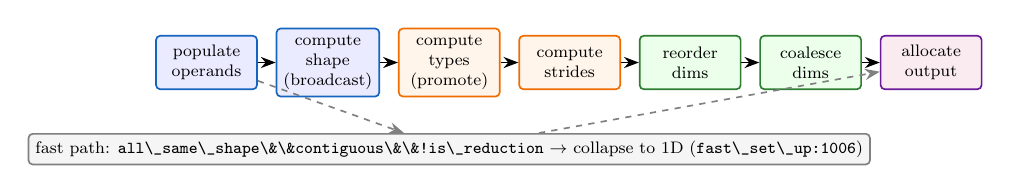
\begin{tikzpicture}[node distance=0.35cm, every node/.style={font=\scriptsize}]
\node[libbox, fill=blue!8, draw=tpblue, minimum width=1.7cm, minimum height=0.9cm, align=center] (a) {populate\\operands};
\node[libbox, fill=blue!8, draw=tpblue, right=0.3cm of a, minimum width=1.7cm, minimum height=0.9cm, align=center] (b) {compute\\shape\\(broadcast)};
\node[libbox, fill=orange!8, draw=tporange, right=0.3cm of b, minimum width=1.7cm, minimum height=0.9cm, align=center] (c) {compute\\types\\(promote)};
\node[libbox, fill=orange!8, draw=tporange, right=0.3cm of c, minimum width=1.7cm, minimum height=0.9cm, align=center] (d) {compute\\strides};
\node[libbox, fill=green!8, draw=tpgreen, right=0.3cm of d, minimum width=1.7cm, minimum height=0.9cm, align=center] (e) {reorder\\dims};
\node[libbox, fill=green!8, draw=tpgreen, right=0.3cm of e, minimum width=1.7cm, minimum height=0.9cm, align=center] (f) {coalesce\\dims};
\node[libbox, fill=purple!8, draw=tppurple, right=0.3cm of f, minimum width=1.7cm, minimum height=0.9cm, align=center] (g) {allocate\\output};
\draw[arrow] (a) -- (b); \draw[arrow] (b) -- (c); \draw[arrow] (c) -- (d); \draw[arrow] (d) -- (e); \draw[arrow] (e) -- (f); \draw[arrow] (f) -- (g);
\node[libbox, fill=gray!8, draw=gray, below=0.6cm of c, minimum width=9.5cm, align=center] (fast) {fast path: \path{all\_same\_shape \&\& contiguous \&\& !is\_reduction} $\rightarrow$ collapse to 1D (\path{fast\_set\_up:1006})};
\draw[arrow, dashed, color=gray] (a) -- (fast); \draw[arrow, dashed, color=gray] (fast) -- (g);
\end{tikzpicture}
\caption{TensorIterator build pipeline. Fast path skips reorder and coalesce for the contiguous case.}
\label{fig:tibuild}
\end{figure}

\begin{enumerate}[leftmargin=1.2em]
\item \textbf{populate\_operands:} move \texttt{Tensor} into \texttt{OperandInfo}, record \texttt{data} and \texttt{stride\_bytes}.
\item \textbf{compute\_shape} (\path{infer\_size:45}): broadcast rule \texttt{size==1} broadcasts, else equal; preserves \texttt{0}-size.
\item \textbf{compute\_types} (\path{compute\_common\_dtype:185} folds \texttt{promoteTypes}, \path{compute\_types:210}): if \path{promote\_inputs\_to\_common\_dtype}, creates temporaries via \path{op.tensor().to(common\_dtype)}; if \path{cast\_common\_dtype\_to\_outputs}, allocates temp output.
\item \textbf{compute\_strides + reorder\_dimensions:106}: insertion sort dims by stride ascending, reduced dims front; disabled if \path{enforce\_linear\_iteration}.
\item \textbf{coalesce\_dimensions:530}: merges \path{shape[n]*stride[n]==stride[n+1]} adjacent dims.
\item \textbf{allocate\_or\_resize\_outputs}: \path{empty(shape, dtype, device)} if \texttt{resize\_outputs}.
\item \textbf{post:} fill \path{op.data = tensor().data\_ptr()}.
\end{enumerate}

\path{fast\_set\_up:1006} collapses to \texttt{shape[0]=numel} when all operands share shape and are contiguous.

\subsection{Type Promotion Lattice}

\path{p10/include/TypePromotion.h:12} defines a strict lattice (\path{Complex $>$ Float $>$ Int $>$ Bool}):

\begin{lstlisting}[caption={\path{TypePromotion.h:12} — lattice (abridged).}, label=lst:promote]
DType promoteTypes(DType a,DType b){
  if(a==b) return a; if(a==Undefined||b==Undefined) return Undefined;
  if(isComplexType(a)||isComplexType(b)){
    if(a==ComplexDouble||b==ComplexDouble) return ComplexDouble;
    if(a==ComplexFloat||b==ComplexFloat) return isFloatingType(other)? ComplexDouble: ComplexFloat;
  }
  if(isFloatingType(a)||isFloatingType(b)){
    if(a==Float64||b==Float64) return Float64; if(a==Float32||b==Float32) return Float32;
    if(a==Float16 && b==BFloat16) return Float32; // avoid mutual loss
  }
  if(a==Bool) return b; if(b==Bool) return a;
  if(a==Int64||b==Int64) return Int64;
}
\end{lstlisting}

\path{DType.h:53} enumerates 20+ types (\texttt{UInt8}, \texttt{Float32}, \texttt{BFloat16}, \texttt{ComplexDouble}, \texttt{QInt8}, ...), with \path{isIntegral/isFloating/isComplex} predicates and \texttt{elementSize}. The result is written to \texttt{Edge::grad\_dtype} for backward cast-back (\path{Engine:498}).

\begin{figure}[H]
\centering
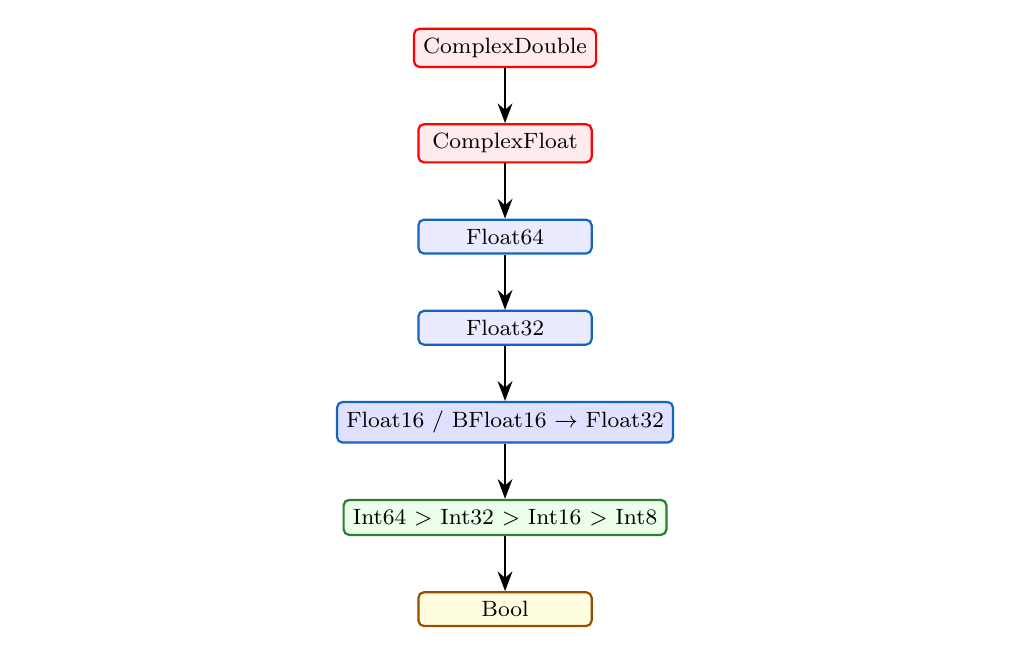
\begin{tikzpicture}[every node/.style={font=\scriptsize}, node distance=0.7cm]
\node[libbox, fill=red!8, draw=red, minimum width=2.2cm] (c) {ComplexDouble};
\node[libbox, fill=red!8, draw=red, below=of c, minimum width=2.2cm] (cf) {ComplexFloat};
\node[libbox, fill=blue!8, draw=tpblue, below=of cf, minimum width=2.2cm] (f64) {Float64};
\node[libbox, fill=blue!8, draw=tpblue, below=of f64, minimum width=2.2cm] (f32) {Float32};
\node[libbox, fill=blue!12, draw=tpblue, below=of f32, minimum width=2.2cm] (f16) {Float16 / BFloat16 $\rightarrow$ Float32};
\node[libbox, fill=green!8, draw=tpgreen, below=of f16, minimum width=2.2cm] (i) {Int64 $>$ Int32 $>$ Int16 $>$ Int8};
\node[libbox, fill=yellow!12, draw=orange!60!black, below=of i, minimum width=2.2cm] (b) {Bool};
\draw[arrow] (c) -- (cf); \draw[arrow] (cf) -- (f64); \draw[arrow] (f64) -- (f32); \draw[arrow] (f32) -- (f16); \draw[arrow] (f16) -- (i); \draw[arrow] (i) -- (b);
\end{tikzpicture}
\caption{Promotion lattice. \path{Float16+BFloat16 $\rightarrow$ Float32} is the special case at \path{TypePromotion.h:84}.}
\label{fig:promotion}
\end{figure}

\subsection{Parallel and Reduction}

\path{TensorIteratorBase:327} \path{for\_each(loop, grain=GRAIN\_SIZE)} dispatches to \path{parallel::parallel\_for} (custom thread pool, \texttt{GRAIN\_SIZE=32768}). \path{TensorIteratorReduce.cpp:33} \texttt{parallel\_reduce} selects \path{two\_pass\_reduction} for single-element outputs (per-thread buffer then \texttt{final\_reduce}) vs.\ \path{parallel\_dim\_reduction:78} (\texttt{find\_split\_dim}, \texttt{narrow}, \texttt{foreach}).

\subsection{Kernel Wiring}

\path{p10/src/backend/cpu/PointwiseKernels.cpp:108}:

\begin{lstlisting}[caption={Pointwise wiring.}, label=lst:pointwise]
template<Func> Tensor unary_op_kernel(const Tensor& self, Func func, VOp vec){
  Tensor out = empty(shape,dtype,device); Tensor contig=self.contiguous();
  bool vec_ok = vecunary::vec_ready() && vec!=None && (dtype==Float32||Float64);
  switch(dtype){ case Float32: { auto s=contig.data_ptr<float>(); auto d=out.data_ptr<float>();
    if(vec_ok) parallel_for(0,n,8192, [&](b,e){ vec_run(vec,prm,s,d,b,e); });
    else parallel_for(0,n,8192,[&](b,e){ for(i=b;i<e;i++) d[i]=func(s[i]); }); break; } ... }
  return out;
}
\end{lstlisting}

CUDA \texttt{PointwiseKernels.cu} currently hand-writes \texttt{blockIdx*blockDim} grid-stride loops without TI — the known repetition left as future work.

\subsection{Comparison}

\begin{table}[H]
\centering
\caption{TensorIterator design tradeoffs.}
\label{tab:ti_compare}
\small
\begin{tabular}{lll}
\toprule
 & TensorPlay & Broader implementation \\
\midrule
CPU & full TI & full TI \\
CUDA & hand-written & full TI \\
MemoryFormat & bool + enum & full propagation \\
Safety & \texttt{can\_cast}: non-Undefined ok & full safe-cast \\
Vector & \texttt{vecunary} outside TI & inside TI \\
\bottomrule
\end{tabular}
\end{table}

% 08-codegen.tex
\section{代码生成与构建}
\label{sec:codegen}

代码生成是唯一可以保持 479 个 \ac{op} 模式、187 个后向公式、13 个调度键、两个语言表面和 6 个构建工件相互一致而不会出现偏差的机制。合约是两个YAML文件；该引擎是一个由本地模式模型驱动的纯Python生成器；输出是十个分段标头和源代码，它们被编译为普通翻译单元。生成后没有任何内容是手工编辑的：每个工件的第一行读取 \texttt{main.py -- DO NOT EDIT} 并且如果生成器过时，构建将拒绝链接。

\subsection{合约：两个 YAML 文件}

运算符注册表 \texttt{native\_functions.yaml} 有 9\,445 行，当扩展重载和 \texttt{.out} 变体时，在 2\,809 \texttt{- func:} 记录中声明 479 个不同的运算符名称。每个条目绑定五个字段：\texttt{func}（FunctionSchema 字符串）、\texttt{variants}（\texttt{function} 和/或 \texttt{method}）、\texttt{dispatch}（从 \texttt{CPU}、\texttt{CUDA}、\texttt{Composite} 到内核符号的映射）、可选 \texttt{python\_defaults} 和可选 \texttt{device\_check} / \texttt{structured\_delegate} / \texttt{tags}。架构字符串是 C++ 签名、Python 绑定和调度程序密钥表的单一来源。变体决定面：\texttt{function} 成为静态成员 \texttt{Tensor::zeros} 和模块函数 \texttt{tensorplay.zeros}； \texttt{method} 成为实例成员 \texttt{tensor.view}。代表性工厂条目会内联拼写其默认值，例如\ \texttt{func: zeros(int[] size, *, ScalarType dtype=Float32, Device device=cpu, bool requires\_grad=False) -> Tensor} 与 \texttt{variants: function} 和 \texttt{dispatch: \{CPU: zeros\_cpu, CUDA: zeros\_cuda\}}。就地条目具有以下类型的可变性：\texttt{add\_(Tensor(a!) self, Tensor other, Scalar alpha=1) -> Tensor(a!)} 和 \texttt{variants: method}。

为 1\,330 行（标签处为 1\,324 行），其中包含 345 条 \texttt{- name:} 记录，按基本名称分组后可折叠为 187 个向后公式。每个记录都以符号方式命名前向参数梯度： \texttt{name: add(Tensor self, Tensor other, Scalar alpha=1) -> Tensor} 、 \texttt{self: grad} 和 \texttt{other: grad * alpha} 等。\ YAML 从不携带 C++ 类型或调度键；这些是从它引用的本机条目推断出来的。公式可以调用分派的操作 (\texttt{mul}, \texttt{sum\_to\_shape}) 和由为向后节点发射器提供动力的相同表达式 AST 解析的自由函数。随机操作会自动添加 \texttt{nondeterministic\_seeded} 标签，并且 \texttt{Vulkan} 密钥在 CPU 版本上保留保留。

除了自己的 \texttt{*.py} 源之外，这两个文件是 Python 管道允许读取的唯一输入。从结构上检查不变量： \texttt{parse\_native\_yaml} 通过本地模式管道解析同一文件两次，将 \texttt{int64\_t} 规范化为 \texttt{int} ，将 \texttt{Composite} 规范化为 \texttt{CompositeExplicitAutograd} ，并在任何删除的记录、分派投影不匹配、变体不匹配或运算符名称冲突时引发 \texttt{ValueError} 。

\begin{tpnote}[Note: YAML Is the Single Source of Truth---Everything Else Is Derived]
每个生成的表面都是两个 YAML 文件的纯函数。 C++ 签名、Python 绑定、\texttt{.pyi} 存根、调度程序密钥表、向后节点和自动转换注册都是 \emph{derived artifacts}：从相同的 YAML 重新生成始终会重现字节相同的输出，并且 \texttt{DO NOT EDIT} 标头使手动修改可检测到，而不仅仅是阻止。贡献者的实际结果是： \emph{never} 编辑生成的文件以修复编译错误——该修复属于 YAML 或生成器，并将覆盖下一个构建时的手动编辑。单一来源规则使完整性检查变得有意义：它们验证从 YAML 到工件的 \emph{projection} 是完整的和单射的，这只是一个明确定义的声明，因为方向是单向的。
\end{tpnote}

\begin{lstlisting}[caption={and fragments.}, label=lst:yamlfrag, style=pystyle]
- func: add.Tensor(Tensor self, Tensor other, *, Scalar alpha=1) -> Tensor
  variants: function, method
  dispatch: {CPU: add_cpu, CUDA: add_cuda}
  python_defaults: {alpha: 1}
- func: add_.Tensor(Tensor(a!) self, Tensor other, *, Scalar alpha=1) -> Tensor(a!)
  variants: method
  dispatch: {CPU: add__cpu, CUDA: add__cuda}
  device_check: NoCheck   # lists checked element-wise elsewhere
- name: add(Tensor self, Tensor other, Scalar alpha=1) -> Tensor
  self: grad * alpha
  other: grad * alpha
\end{lstlisting}

\subsubsection{YAML 合同完整性检查：\texttt{parse\_native\_yaml}}

\texttt{parse\_native\_yaml} 是 YAML 文本和每个生成器之间的单一门户。它执行七项结构检查，共同保证合同的完整性和单射性。该实现加载文件两次：一次通过本地模型的 \texttt{YamlLoader}，一次通过独立的结构验证路径。没有模式可以绕过第二次解析。

\begin{table}[H]
\centering
\caption{完整性检查和--\texttt{752}。}
\label{tab:yaml_checks}
\small
\begin{tabular}{lll}
\toprule
查看 & Site & 失败 \\
\midrule
删除记录 &  & \texttt{ValueError: schema parser dropped records} if \texttt{len(parsed) < len(prepared)} \\
重复运算符 & , \texttt{1026} & \texttt{duplicate parsed operator schema} / \texttt{duplicate operator schema \{func\_name\}} \\
缺失/额外 &  & \texttt{record set mismatch: missing=\dots extra=\dots} \\
模式投影 &  & \texttt{schema projection mismatch: \{actual\} != \{预期\}} \\
模式种类 &  & \texttt{mutable} \\
变体集 &  & \texttt{variant mismatch: \{actual\} != \{预期\}} \\
调度投影 &  & \texttt{dispatch projection mismatch: \{actual\} != \{预期\}} \\
\bottomrule
\end{tabular}
\end{table}

具体来说，\texttt{\_prepare\_schema\_entry} 在验证之前规范化每个项目：它剥离 \texttt{python\_defaults}，将 \texttt{int64\_t} 重写为 \texttt{int}，将 \texttt{Composite} 提升为 \texttt{CompositeExplicitAutograd}，为名称包含 \texttt{rand} 或参数包含 \texttt{dropout} ( \texttt{\_requires\_seeded\_tag}) 的任何模式注入 \texttt{nondeterministic\_seeded}，并为工厂合成 \texttt{CompositeExplicitAutograd} 调度 (\texttt{new\_*} / \texttt{*\_like} / 仅 TensorOptions）通过 \texttt{cpp.name}。 \texttt{\_validate\_dispatch\_projection} 然后根据 \texttt{backend\_metadata} 验证 YAML \texttt{dispatch} 映射；仅忽略 \texttt{\_\_line\_\_}。 \texttt{\_validate\_native\_projection} 为本地 \texttt{NativeFunction} 断言四个相等：字符串化 \texttt{FunctionSchema}、\texttt{SchemaKind} (\texttt{functional} / \texttt{inplace} / \texttt{mutable})、变体名称集和 \texttt{cpp\_no\_default\_args} 集。顶级 \texttt{parse\_native\_yaml} 循环通过 \texttt{seen\_schemas} 删除精确重复的 \texttt{- func:} 字符串（合并工件），但将解析为相同 \texttt{func\_name} （过载冲突）的任何两个不同字符串视为错误。最后，设置相等可确保没有名称丢失或多余。

\begin{lstlisting}[caption={Completeness check diagnostics (abridged from --\texttt{1044}).}, label=lst:yamlchecks, style=pystyle]
# model.py:707  dispatch mismatch
raise ValueError(f"dispatch projection mismatch for {f.func_name}: "
                 f"{actual} != {expected}")
# model.py:982  dropped records
raise ValueError(f"schema parser dropped records for {path}: "
                 f"{len(prepared)} > {len(parsed.native_functions)}")
# model.py:1038 record set mismatch
if configured_names != reference_names:
    raise ValueError(f"schema parser record set mismatch: "
                     f"missing={missing[:8]} extra={extra[:8]}")
\end{lstlisting}

\subsection{架构模型：（1\,055 行）}

模型层是本地模式记录的薄投影。 \texttt{\_ensure\_schema\_model} 加载解析器模块并缓存该模块。 \texttt{parse\_schema} 用 \texttt{int} 替换 \texttt{int64\_t}，恢复仅关键字参数，并通过 \texttt{\_type\_from\_tg} 将每个解析的类型映射到本地 \texttt{Type} 记录。 \texttt{Type} 存储 \texttt{kind}、\texttt{is\_list}、\texttt{is\_opt}、\texttt{mutability} 和 \texttt{list\_elem\_opt}；助手 \texttt{is\_tensor\_like}、\texttt{is\_mutable\_ref} 和 \texttt{is\_mutable\_tensor\_list} 驱动下游的可变性处理。

\texttt{NativeFunction} 携带 \texttt{schema}、\texttt{base\_name}、\texttt{cpp\_name}、\texttt{overload\_name}、\texttt{args: list[Argument]}、\texttt{returns: list[ReturnDecl]}、\texttt{variants}、\texttt{dispatch}、\texttt{device\_check}、\texttt{structured\_delegate}、\texttt{pydefaults}、\texttt{schema\_kind} (\texttt{functional} / \texttt{inplace} / \texttt{mutable})、\texttt{tags} 和 \texttt{backend\_metadata}。视图元数据（\texttt{is\_view\_op}、\texttt{returns\_view\_of\_input}、\texttt{view\_input\_name}）是通过 \texttt{\_ensure\_view\_metadata} 从 \texttt{tools.autograd.gen\_inplace\_or\_view\_type} 延迟加载的。 \texttt{\_native\_function\_from\_yaml} 将本地 YAML 字段合并到引用函数上，设置 \texttt{cpp\_no\_default\_args}，并在将 \texttt{Composite} 规范化为 \texttt{CompositeExplicitAutograd} 后验证调度映射。 \texttt{NativeFunctionCollection} 包装结果列表，并使用与参考生成器相同的预分组公开 \texttt{grouped\_native\_functions} 和 \texttt{grouped\_view\_functions} ，因此下游生成器看到与规范构建相同的 function/out 和 view/view\_copy/view\_inplace 组。

\subsubsection{\texttt{parse\_schema} 通过模式模型}

\texttt{parse\_schema} 是存储库中 FunctionSchema 的唯一拼写。它委托给本地解析器，同时保留本地不变量。步骤：

\begin{enumerate}[nosep, leftmargin=1.2em]
\item 将解析器的 \texttt{int64\_t} 标准化为 \texttt{int}，而本地 \texttt{Type.kind} 通过 \texttt{\_KIND\_ALIASES} 保留 \texttt{int64\_t}。
\item 调用 \texttt{tgm.FunctionSchema.parse} 并断言往返保真度（： \texttt{str(ts) != schema} 引发）。
\item 从 \texttt{ts.arguments.flat\_kwarg\_only} 恢复仅关键字状态，因为 \texttt{ts.arguments.all} 展平了三个存储桶。
\item 按架构顺序将 \texttt{TensorOptionsArguments} 包装器 (\texttt{expand}) 展开为四个组成部分 \texttt{dtype}/\texttt{layout}/\texttt{device}/\texttt{pin\_memory} 参数。
\item 通过 \texttt{\_type\_from\_tg} 映射每个 \texttt{tgm} 类型，该 \texttt{\_type\_from\_tg} 剥离 \texttt{OptionalType} / \texttt{ListType}，检测 \texttt{list\_elem\_opt}，并应用 \texttt{\_KIND\_ALIASES}（\texttt{SymInt} $\rightarrow$ \texttt{int64\_t} 反转）。
\item 实现可变性：当 \texttt{tgm} 注释被写入（ \texttt{a.annotation.is\_write}）且类型为 \texttt{Tensor} 时，用 \texttt{mutability="a"} 重新创建 \texttt{Type} ，因此 \texttt{is\_mutable\_ref} 和 \texttt{is\_mutable\_tensor\_list} 为 true。
\item 当架构已包含 \texttt{input} 时，对带有数字后缀的面向 Python 的重命名 \texttt{self} $\rightarrow$ \texttt{input} 进行重复数据删除。
\end{enumerate}

\begin{table}[H]
\centering
\caption{\texttt{Type} 字段由 \texttt{\_type\_from\_tg} 生成。}
\label{tab:typefields}
\small
\begin{tabular}{lll}
\toprule
场地 & Type & 意义 \\
\midrule
\texttt{kind} & \texttt{str} & \texttt{Tensor}, \texttt{Scalar}, \texttt{DType}, \texttt{Device}, \texttt{int64\_t}, \texttt{double}, \texttt{bool} \\
\texttt{is\_list} & \texttt{bool} & \texttt{true} 代表 \texttt{Tensor[]}、\texttt{int[]}、\texttt{bool[3]} \\
\texttt{is\_opt} & \texttt{bool} & \texttt{true} 代表 \texttt{Tensor?}、\texttt{int?} \\
\texttt{mutability} & \texttt{str | None} & \texttt{"a"} 表示 \texttt{Tensor(a!)}、\texttt{"a!"} 携带参数 \\
\texttt{list\_elem\_opt} & \texttt{bool} & \texttt{true} 代表 \texttt{Tensor?[]} \\
\texttt{list\_size} & \texttt{int | None} & 固定变量的 \texttt{[N]} 或 \texttt{None} \\
\bottomrule
\end{tabular}
\end{table}

\begin{lstlisting}[caption={\texttt{\_type\_from\_tg} and return-kind classification.}, label=lst:parse_schema, style=pystyle]
def _type_from_tg(t) -> Type:          # model.py:203
    is_opt = isinstance(t, tgm.OptionalType)
    inner = t.elem if is_opt else t
    is_list = isinstance(inner, tgm.ListType)
    elem = inner.elem if is_list else inner
    list_elem_opt = isinstance(elem, tgm.OptionalType)
    # ... kind via _KIND_ALIASES, symint/symbool/symfloat ...
    return make_type(kind, is_list, is_opt, None, symint, ...)

# model.py:313 cpp_return_kind
# 0 ret or void -> "void"; >1 ret -> "tuple"
# 1 ret list    -> "list";  1 ret Tensor(a!) -> "mut_ref" else "value"
\end{lstlisting}

\subsection{编排器：（253行）}

定义协调器。 \texttt{CodegenContext} 保存 \texttt{funcs}、\texttt{native\_by\_opname}、\texttt{derivatives}、\texttt{autocast\_ops}、\texttt{autograd\_ops}（将调度程序名称映射到后向节点名称，\texttt{relu\_} 默认为 \texttt{ReluBackward}）、\texttt{out\_dir}、\texttt{pkg\_out}、\texttt{backend\_indices}、\texttt{reference\_functions} 和 \texttt{written}。 \texttt{register\_generator} 填充全局 \texttt{\_GENERATORS} 字典。每个生成器都是一个普通函数，它接收上下文并调用 \texttt{ctx.write} 或 \texttt{ctx.write\_pkg}。 \texttt{DEFAULT\_TARGETS} 列出了默认的十一个：

\begin{table}[H]
\centering
\caption{生成器和工件。每个都通过 \texttt{model.py} 模式投影读取 YAML。行数为 \texttt{*.py}。}
\label{tab:codegen_generators}
\small
\begin{tabular}{llll}
\toprule
目标 & 模块 & 输出 & 核心入门 \\
\midrule
张量方法 &  & \texttt{.cpp} & \texttt{generate\_header}, \texttt{generate\_cpp} \\
重新调度 &  & \texttt{TensorRedispatchGenerated.h} & \texttt{generate\_redispatch\_header} \\
Autograd节点 &  & \texttt{AutogradNodesGenerated.h} & \texttt{generate\_autograd\_nodes} \\
TPX操作 &  & \texttt{.cpp} & \texttt{cpp} \\
自动微分注册 &  & \texttt{TPXAutogradRegistration.cpp} & \texttt{generate\_autograd\_registration} \\
绑定 &  & \texttt{TensorBindingsGenerated.h} & \texttt{generate\_bindings} \\
自动转换 &  & \texttt{AutocastGenerated.cpp} & \texttt{generate\_autocast\_registration} \\
PythonCAPI &  & \texttt{TensorCPythonGenerated.h} & \texttt{\_gen\_python\_capi} \\
结构化 &  & \texttt{StructuredGenerated.h} & \texttt{\_gen\_structured} \\
就地或查看 &  & \texttt{InplaceOrViewGenerated.h} & \texttt{\_gen\_inplace\_or\_view} \\
Python函数式 &  & \texttt{functional.py} & \texttt{generate\_functional\_py} \\
Pyi存根 &  & \texttt{*.pyi} & \texttt{generate\_pyi} \\
\bottomrule
\end{tabular}
\end{table}

CLI 接受 \texttt{--yaml}、\texttt{--derivatives}、\texttt{--out\_dir}、\texttt{--pkg\_out}、\texttt{--pyi\_template}、\texttt{--pyi\_out} 和 \texttt{--targets}（以逗号分隔，默认为 \texttt{DEFAULT\_TARGETS}）。验证未知目标，通过 \texttt{parse\_native\_yaml} 解析 YAML，通过 \texttt{gen\_autograd.load\_derivatives} 加载衍生品，查询 \texttt{autocast\_registered\_ops}，构建上下文，并分派 \texttt{run\_gen} 按顺序迭代目标。因为每个生成器共享一个 \texttt{NativeFunctionCollection} 和一个 \texttt{derivatives} 字典，所以参数名称、默认值和调度键不能不同。

\subsubsection{ \texttt{CodegenContext}}

\texttt{CodegenContext} 是一个数据类，它通过所有十二个生成器进行单个解析。领域：

\begin{table}[H]
\centering
\caption{\texttt{CodegenContext} 字段。}
\label{tab:codegencontext}
\small
\begin{tabular}{lll}
\toprule
场地 & Type & Role \\
\midrule
\texttt{funcs} & \texttt{NativeFunctionCollection} & 有序列表 + \texttt{grouped\_native\_functions} 视图 \\
\texttt{native\_by\_opname} & \texttt{dict[func\_name $\rightarrow$ NativeFunction]} & 按调度程序名称键入的派生查找 \\
\texttt{derivatives} & \texttt{dict[op $\rightarrow$ OpDerivatives]} & 187 个向后公式 + \texttt{relu\_} 默认值 \\
\texttt{autocast\_ops} & \texttt{set[str]} & 使用 \texttt{CUDA} 内核的操作 \\
\texttt{autograd\_ops} & \texttt{dict[str,str]} & \texttt{func\_name $\rightarrow$ node\_name} \\
\texttt{out\_dir} & \texttt{str} & \texttt{GEN\_INCLUDE\_DIR} 代表 \texttt{ctx.write} \\
\texttt{pkg\_out} & \texttt{str | None} & \texttt{TP\_PACKAGE\_DIR} 代表 \texttt{ctx.write\_pkg} \\
\texttt{backend\_indices} & \texttt{dict} & 用于结构化检查的每键调度索引 \\
\texttt{reference\_functions} & \texttt{tuple} & 用于分组的解析器记录 \\
\texttt{written} & \texttt{dict[str,str]} & 文件名 $\rightarrow$ 新鲜度测试路径 \\
\bottomrule
\end{tabular}
\end{table}

两个属性组函数：\texttt{grouped\_native\_functions} 通过 \texttt{NativeFunctionsGroup.from\_dict} 对函数/输出变体进行分组； \texttt{grouped\_view\_functions} 对别名组 (\texttt{view} / \texttt{view\_copy} / \texttt{view\_inplace}) 执行相同的操作。两个方法抽象I/O：\texttt{write}连接\texttt{out\_dir}，确保父目录，写入并记录\texttt{written}； \texttt{write\_pkg} 在 \texttt{pkg\_out} 下执行相同的操作并断言它已设置。 \texttt{backend\_index} 通过 \texttt{name} 字符串相等性来解析调度键。

\subsubsection{ \texttt{DEFAULT\_TARGETS}}

\texttt{DEFAULT\_TARGETS} 枚举在每个 \texttt{cmake --build} 上运行的十一个目标：

\begin{lstlisting}[caption={default target list.}, label=lst:defaulttargets, style=pystyle]
DEFAULT_TARGETS = ["TensorMethods", "Redispatch", "AutogradNodes", "TPXOps",
                   "AutogradRegistration", "Bindings", "Autocast",
                   "InplaceOrView", "Structured", "PythonFunctional",
                   "PythonCAPI"]
\end{lstlisting}

\texttt{PyiStub} 是第十二个注册的生成器（\texttt{\_gen\_pyi}），但被排除在 \texttt{DEFAULT\_TARGETS} 之外，因为它通过 \texttt{ctx.pyi\_out} 写入源码包目录并需要 \texttt{--pyi\_template} / \texttt{--pyi\_out}。 CLI 默认 \texttt{--targets} 到 \texttt{",".join(DEFAULT\_TARGETS)} 并使用 \texttt{SystemExit(unknown generators)} 验证未知名称。顺序是承载的： \texttt{TensorMethods} before \texttt{Redispatch} before \texttt{TPXOps} 确保在发出 autograd 包装器时存在重新调度标头； \texttt{run\_gen} 按列出的顺序迭代，并通过由 \texttt{register\_generator} 填充的全局 \texttt{\_GENERATORS} 字典调用每个函数。每个生成器都会收到相同的 \texttt{CodegenContext}，因此 YAML 中的重命名会自动传播到所有工件，而无需按目标重新解析。

\subsection{张量曲面：（718 线）}

每个操作员都获得两个表面：一个通过调度程序解析内核的后端重新调度漏斗，以及一个公共 \texttt{Tensor} 成员，该成员在进入重新调度之前执行检查和转换调度。两者均从 \texttt{gen\_api.py} 发出。

\subsubsection{超载计划：\texttt{plan\_members}}

C++ 不能单独重载返回类型、默认值或常量。 \texttt{\_overload\_key} 在剥离 \texttt{requires\_grad} 后将变体折叠为 \texttt{(cpp\_name, tuple(cpp\_arg\_type))}，对于 \texttt{method}，则折叠为 \texttt{self}。当两个成员共享参数类型的公共前缀并且超过该前缀的每个参数都是双方默认的时，\texttt{\_prefix\_ambiguous} 认为两个成员发生冲突；仅提供前缀的调用对于两者都是可行的，并且重载解析将是不明确的。 \texttt{\_HANDWRITTEN\_TENSOR\_METHODS} 列出了（\texttt{dim}、\texttt{numel}、\texttt{detach}、\texttt{as\_strided}、\texttt{to} 等）拥有的成员；手写的无参数成员加上生成的带默认值的单参数成员会产生相同的歧义，因此手写的所有者获胜。 \texttt{plan\_members} 按 YAML 顺序迭代模式，记录每个 \texttt{cpp\_name} 发出的参数列表，并在新变体发生冲突或手写时将 \texttt{plan[(func\_name, variant)]} 标记为 false。 \texttt{generate\_header} 和 \texttt{generate\_cpp} 都会查阅该地图，因此被抑制的成员仍然保留其重新调度帮助程序和注册条目。

\begin{table}[H]
\centering
\caption{\texttt{plan\_members} 决策表。}
\label{tab:planmembers}
\small
\begin{tabular}{lll}
\toprule
健康）状况 & Test & 影响 \\
\midrule
手写业主 & \texttt{cpp\_name in \_HANDWRITTEN\_TENSOR\_METHODS} & \texttt{plan[func,variant]=False} \\
前缀歧义 & \texttt{\_prefix\_ambiguous(prev, new)} & 后来的变种被抑制 \\
精确类型冲突 & \texttt{\_overload\_key} 已经在 \texttt{seen\_decl} 中 & 重复数据删除，不排放 \\
否则 & YAML顺序，先胜 & \texttt{plan[func,variant]=True} \\
\bottomrule
\end{tabular}
\end{table}

\subsubsection{标头发射：\texttt{generate\_header}}

\texttt{generate\_header} 将 \texttt{TensorGenerated.h} 写在 \texttt{\#pragma once} 下，并带有 \texttt{\#include <tuple>}。它重播 \texttt{plan\_members}，对 \texttt{\_overload\_key} 进行重复数据删除，并为 \texttt{function} 变体（工厂表面 \texttt{Tensor::zeros}）和实例成员发出 \texttt{static}，否则，当 \texttt{self} 不是 \texttt{a!} 时，通过 \texttt{\_is\_const\_method} 附加 \texttt{const}。签名由 \texttt{method\_signature} 使用 \texttt{api\_types.cpp\_return\_type} 和 \texttt{cpp\_arg\_type} 渲染，默认值来自 \texttt{cpp\_default}，除非 \texttt{cpp\_no\_default\_args} 抑制它们或操作是 \texttt{.out}。结果是一个标头被设计为包含在 \texttt{class Tensor} (\S\ref{sec:codegen_class_mixing}) 内，而不是包含在命名空间范围内。

\subsubsection{设备和密钥解析：\texttt{\_device\_source} 和 \texttt{\_dispatch\_key\_expr}}

\texttt{\_device\_source} 对于一种架构和变体返回 \texttt{(dispatch\_key\_source, target\_device\_expr)}。如果存在 \texttt{device} 参数，则直接使用它，对于 \texttt{\_like} 工厂，可选设备回退到 \texttt{Device(DeviceType::CPU)} 或 \texttt{self.device} ；对于 \texttt{method} 变体，\texttt{device} 表示 \texttt{self.device}，稍后在自由函数重新调度中重写为 \texttt{self.device}。否则第一个非可选 \texttt{Tensor}，然后通过 \texttt{deviceForTensorArg} 第一个 \texttt{Tensor[]}，否则为 CPU。 \texttt{\_dispatch\_key\_expr} 选择最高的活动变换键：\texttt{copy\_} 使用其第一个参数，\texttt{\_RANDOM\_TRANSFORM\_OPS} 中的随机工厂使用 \texttt{transform::dispatch\_key\_for\_random(computeDispatchKey(device))}，并且一般情况会在每个类似张量的参数上折叠 \texttt{dispatchKeyForTensorArgs(self, a, b)} （方法接收器在重新调度外部变为 \texttt{*this}，在内部变为 \texttt{self}）。

\subsubsection{重新调度漏斗：\texttt{\_emit\_redispatch} 和 \texttt{OpRecord}}

\texttt{\_emit\_redispatch} 在 \texttt{namespace detail} 下为每个模式发出一个自由函数 \texttt{detail::redispatch\_<op>\_<variant>}：

\begin{lstlisting}[caption={skeleton of \texttt{\_emit\_redispatch} (simplified).}, label=lst:emitredispatch, style=cppstyle]
namespace detail {
TENSORPLAY_API Tensor redispatch_add_Tensor_method(const Tensor& self,
                                                   const Tensor& other, Scalar alpha) {
    tensorplay::prof::OpRecord __tp_prof_rec("add.Tensor");
    if (tensorplay::prof::g_capture_shapes.load(std::memory_order_acquire)) {
        // capture shapes/dtypes of Tensor-like args into __tp_prof_shapes
    }
#ifdef USE_CUDA
    tensorplay::prof::GpuTimerPair __tp_gpu(__tp_prof_rec);
#endif
#ifdef USE_CUDA
    cuda::OptionalCUDAGuard device_guard(self.device());
#endif
    static const OperatorHandle op_handle =
        Dispatcher::singleton().findHandle("add.Tensor");
    DispatchKey dispatch_key = toBackendKey(dispatchKeyForTensorArgs(self));
#ifdef USE_CUDA
    __tp_gpu.arm(self.device());
#endif
    auto&& __tp_result = DispatchStub<Tensor,const Tensor&,const Tensor&,Scalar>
        ::call(op_handle, dispatch_key, self, other, alpha);
#ifdef USE_CUDA
    __tp_gpu.close();
#endif
    // output allocation volume and version bump handled below
    return std::move(__tp_result);
}
} // namespace detail
\end{lstlisting}

具体来说，发射器写入：由 \texttt{func\_name} 键控的 \texttt{OpRecord}，由 \texttt{g\_capture\_shapes} 保护的形状捕获分支，枚举 \texttt{Tensor}、\texttt{Tensor[]}、\texttt{Tensor?} 和 \texttt{Tensor?[]}，一个 \texttt{GpuTimerPair} 池支持的 \texttt{cudaEvent} 对，当 \texttt{device\_guard} 为 true 时的 \texttt{OptionalCUDAGuard}，通过 \texttt{Dispatcher::singleton.findHandle(func\_name)} 解析一次的 \texttt{static const OperatorHandle}，由 \texttt{\_dispatch\_key\_expr} 计算出的 \texttt{DispatchKey} 和用于非随机操作的 \texttt{toBackendKey}，在分派前有 \texttt{\_\_tp\_gpu.arm(device)} ，在分派后有 \texttt{\_\_tp\_gpu.close} ，通过句柄键入的 \texttt{DispatchStub<Ret,Args...>::call} ，以及每个可变参数的版本碰撞：由 \texttt{!InferenceMode::is\_enabled} 保护的 \texttt{unsafeGetTensorImpl->bump\_version} ，在 \texttt{Tensor(a!)} 数组上有列表可变循环。主体是分析器的单个每操作检测点。

\begin{table}[H]
\centering
\caption{\texttt{\_emit\_redispatch} 发射顺序。}
\label{tab:emitredispatch}
\small
\begin{tabular}{lll}
\toprule
Step & 线路 & Code \\
\midrule
1 个操作记录 &  & \texttt{OpRecord \_\_tp\_prof\_rec("func\_name")} \\
2 形状捕捉 & --\texttt{389} & \texttt{g\_capture\_shapes} $\rightarrow$ \texttt{set\_io\_meta(shapes,dtypes)} \\
3 Gpu定时器对 &  & \texttt{GpuTimerPair \_\_tp\_gpu(\_\_tp\_prof\_rec)} \\
4 设备防护 &  & \texttt{OptionalCUDAGuard(device)} \\
5 手柄 &  & \texttt{static OperatorHandle = findHandle(func\_name)} \\
6 调度密钥 &  & \texttt{toBackendKey(dispatchKeyForTensorArgs(\dots))} \\
7 派遣 &  & \texttt{DispatchStub<Ret,Args>::call(handle,key,args)} \\
8 版本碰撞 &  & \texttt{bump\_version} 每 \texttt{Tensor(a!)} \\
\bottomrule
\end{tabular}
\end{table}

\subsubsection{热心会员：\texttt{generate\_cpp} 和设备卫士}

\texttt{generate\_cpp} 运行两次。 Pass~1 发出在 \texttt{redispatch\_key} 上进行重复数据删除的重新调度渠道。 Pass~2 发出公共 \texttt{Tensor} 成员，在 \texttt{\_overload\_key} 上进行重复数据删除并通过 \texttt{plan\_members} 进行过滤。每个成员都是合格的 \texttt{Tensor::} 并以特殊情况的快速路径打开：\texttt{copy\_} 验证 \texttt{shape} 相等性，\texttt{contiguous} 解析 \texttt{MemoryFormat::Preserve} 并在已经连续时返回 \texttt{*this} 以避免用 \texttt{ContiguousBackward} 节点标记叶别名。 \texttt{\_emit\_device\_checks} 如下：标量 \texttt{Tensor} 和 \texttt{Tensor?} 发出 \texttt{if (a.device != target) TP\_THROW(DeviceMismatchError,\dots)}； \texttt{Tensor[]} 循环元素并报告有问题的参数名称。对于目标设备为目标的 \texttt{device\_check == NoCheck} 和 \texttt{copy\_} ，将跳过检查。

成员内部键的顺序是承重的。设备检查后，首先探测偏移量~9处的vmap：计算\texttt{\_\_tp\_key = dispatchKeyForTensorArgs(...)}，测试\texttt{is\_vmap\_key}，如果没有注册批处理规则，则通过带有\texttt{NotImplementedError}的vmap句柄直接\texttt{DispatchStub::call}。 Autocast 是第二个：计算 \texttt{\_\_ac\_key = toAutocastKey(computeDispatchKey(dev\_src))}，在探测 \texttt{getKernel} 之前检查 \texttt{autocast::is\_enabled}，如果存在则调度。 Autograd 是第三个：\texttt{autograd\_ops} 将 \texttt{func\_name} 映射到后向节点名称，并且当 \texttt{GradMode::is\_enabled} 和内核注册时，成员通过 \texttt{toAutogradKey} 调度。如果没有任何转换键触发，则尾部调用 \texttt{detail::redispatch\_<op>\_<variant>}。

\subsubsection{重新调度标头：\texttt{generate\_redispatch\_header}}

\texttt{generate\_redispatch\_header} 将 \texttt{TensorRedispatchGenerated.h} 与 \texttt{\#include "Tensor.h"} 和 \texttt{\#include "Macros.h"} 写入 \texttt{namespace tensorplay::detail} 内，并声明每个 \texttt{TENSORPLAY\_API Ret redispatch\_<op>\_<variant>(stub\_args)} 一次。该标头由 eager 编译单元和 autograd 包装器包含，以便 autograd 层可以调用相同的分派内核，而无需重新解析句柄。

\subsection{Autograd 曲面：（624 线）}

\texttt{gen\_tpx.py} 产生位于 \texttt{tpx} 中的 \texttt{AutogradCPU}/\texttt{AutogradCUDA} 内核。每个算子都通过自动转换、突变防护、后端和后向节点构造来公开 \texttt{tensorplay::tpx::ops::<name>} 路由。

\subsubsection{内联谓词：\texttt{\_inline\_forward\_lines} vs.\ 非内联}

\texttt{\_inline\_forward\_lines} 决定包装器是否不进行急切路径工作并且可以作为内联标头定义发出。当操作符没有向后（\texttt{\_has\_autograd}，包括手动关闭的 \texttt{relu\_}）、没有自动转换规则、没有 \texttt{device} 或 \texttt{dtype} 的工厂全局默认解析（当包装器必须填充 \texttt{DType} 时）、没有视图版本计数器共享以及没有 \texttt{requires\_grad} 管道时，它返回一个主体。否则，它返回 \texttt{None} 并强制在 \texttt{TPXOpsGenerated.cpp} 中出现一个外线主体。核心调用表达式 \texttt{\_core\_call\_expr} 选择 \texttt{::tensorplay::detail::redispatch\_<op>\_<variant>}，或者对于 \texttt{manual\_kernel\_registration}，选择底层 \texttt{Tensor::} 成员。

\begin{table}[H]
\centering
\caption{内联谓词与非内联谓词。}
\label{tab:tpxinline}
\small
\begin{tabular}{lll}
\toprule
健康）状况 & Test & 结果 \\
\midrule
有落后 & \texttt{\_has\_autograd(f,derivatives)} & 非内联 \\
多输出视图 & \texttt{list return + returns\_view\_of\_input + dim} & 非内联 \\
自动转换规则 & \texttt{func\_name in autocast\_ops} & 非内联 \\
出厂设备默认值 & \texttt{device: optional<Device>} 无张量 & 非内联 \\
工厂默认数据类型 & \texttt{dtype in \_DTYPE\_GLOBAL\_DEFAULT\_OPS} & 非内联 \\
查看分享 & \texttt{returns\_view\_of\_input + value} & 非内联 \\
需要等级管道 & \texttt{requires\_grad arg + value} & 非内联 \\
否则 & 普通转发器 & 排队 \\
\bottomrule
\end{tabular}
\end{table}

\begin{lstlisting}[caption={Inline vs.\ non-inline emission.}, label=lst:tpxinline, style=cppstyle]
// gen_tpx.py:137 inline trivial forwarder in TPXOpsGenerated.h
inline Tensor add(const Tensor& self, const Tensor& other, Scalar alpha = 1) {
    return ::tensorplay::detail::redispatch_add_Tensor_function(self, other, alpha);
}
// gen_tpx.py:140 non-inline declaration
TENSORPLAY_API Tensor mm(const Tensor& self, const Tensor& mat2);
// body lives in TPXOpsGenerated.cpp with 5 blocks
\end{lstlisting}

\subsubsection{标头拆分：\texttt{generate\_tpx\_ops\_h}}

\texttt{generate\_tpx\_ops\_h} 对 \texttt{\_dedup\_key}（C++ 名称加上参数类型列表）进行重复数据删除，计算 \texttt{cpp\_return\_type} 和 \texttt{\_signature\_args}，对于 \texttt{inline} 操作直接发出 \texttt{inline Ret name(args) \{ return detail::redispatch(...); \}}；其余的它发出 \texttt{TENSORPLAY\_API Ret name(args);} 作为前向声明。这种分割将热的普通转发器保留在标头中以进行内联，同时将图形构建包装器保留在标头之外。

\subsubsection{包装体：\texttt{generate\_tpx\_ops\_cpp}}

每个外线包装器都遵循相同的五个块。 (1) 工厂全局默认分辨率从 \texttt{globalContext.defaultDevice} 填充 \texttt{device}，对于 \texttt{rand}、\texttt{randn}、\texttt{empty}、\texttt{zeros}、\texttt{ones}、\texttt{dtype}，当调用者未设置它们时，从 \texttt{globalContext.defaultDType} 填充； \texttt{arange}/\texttt{linspace} 被排除，因为它们从标量输入推断数据类型。 (2) 自动转换：\texttt{\_emit\_autocast\_block} 从第一个张量参数重新导出设备源，并在 \texttt{autocast::is\_enabled} 时通过 \texttt{toAutocastKey} 进行调度。 (3)梯度簿记：\texttt{\_emit\_requires\_grad\_detection}从\texttt{GradMode}、\texttt{InferenceMode}以及任何需要梯度的张量中设置\texttt{bool requires\_grad}； \texttt{\_emit\_leaf\_checks} 禁止叶或多输出视图的就地突变；对于派生使用 \texttt{self} 的就地操作，突变前克隆 \texttt{\_\_tp\_original\_self} 在 \texttt{GradMode} 禁用下捕获。 (4) 核心调用按 \texttt{cpp\_return\_kind} (\texttt{value}、\texttt{tuple}、\texttt{list}、\texttt{mut\_ref}、\texttt{void}) 存储 \texttt{core\_result} / \texttt{result}。对于视图操作，包装器共享版本计数器，标记 \texttt{is\_view}，并通过重播 lambda \texttt{\_view\_replay\_lambda} 使用 \texttt{CreationMeta::DEFAULT} 或 \texttt{MULTI\_OUTPUT\_NODE} 安装视图元数据。 (5) 后向节点：\texttt{\_node\_ctor\_args} 从 \texttt{derivatives} 公式中排序构造函数参数，\texttt{\_emit\_edges} 收集 \texttt{Edge}（包括列表类型重载），并且结果按每个返回类型用 \texttt{set\_grad\_fn} / \texttt{set\_requires\_grad} 包装。 \texttt{generate\_autograd\_registration} 然后通过 \texttt{Dispatcher::registerKernel} 为键 \texttt{AutogradCPU}、\texttt{AutogradCUDA}、\texttt{AutogradVulkan} 注册每个包装器一次。

\subsection{剩余发电机}

\texttt{generate\_autograd\_nodes} 通过表达式 AST（分词器加优先级攀爬解析器）而不是正则表达式进行解析，遍历 AST 一次以计算保存的变量集，并写入 \texttt{AutogradNodesGenerated.h}，每个向后节点使用一个结构来保存保存的张量和 \texttt{apply} 主体。 \texttt{generate\_bindings} 写入 \texttt{TensorBindingsGenerated.h} 通过 \texttt{pybind11} 暴露 \texttt{bind\_generated\_tensor\_methods} 和 \texttt{bind\_generated\_op\_functions}，跳过 FASTCALL 层已声明的任何操作。 \texttt{generate\_autocast\_registration} 写入 \texttt{AutocastGenerated.cpp} 注册自动转换内核。并为结构化内核和别名/就地元数据编写单头填充程序；两者都包含在构建的早期，因此调度程序在 Python 扩展链接之前看到它们的内核。

\subsection{构建分期：和}

构建文件定义了暂存合同。 \texttt{GEN\_BASE\_DIR} 默认为 \texttt{generated}，\texttt{GEN\_INCLUDE\_DIR} 默认为 \texttt{ops}。十个变量枚举阶段输出：\texttt{GEN\_HEADER} (\texttt{TensorGenerated.h})、\texttt{GEN\_CPP}、\texttt{GEN\_BINDINGS\_HEADER}、\texttt{GEN\_CPYTHON\_HEADER}、\texttt{GEN\_AUTOGRAD\_NODES\_H}、\texttt{GEN\_TPX\_OPS\_H}、\texttt{GEN\_TPX\_OPS\_CPP}、\texttt{GEN\_TPX\_AUTOGRAD\_REG\_CPP}、\texttt{GEN\_AUTOCAST\_CPP} 和 \texttt{GEN\_TPX\_REDISPATCH\_H}。同一个文件声明一个 \texttt{add\_custom\_command}，其 \texttt{OUTPUT} 是上述所有八个加上绑定头，其\texttt{COMMAND} 是 \texttt{derivatives.yaml --out\_dir GEN\_INCLUDE\_DIR --pkg\_out tensorplay}，\texttt{PYTHONPATH} 是存储库的根目录，其 \texttt{DEPENDS} 列出了两个 YAML 文件、所有 \texttt{*.py} 模块和 \texttt{.cpp}，因此桥接更改会触发重新生成。它标记每个输出 \texttt{GENERATED TRUE} 并创建 \texttt{p10}、\texttt{tpx} 和 \texttt{\_C} 所依赖的虚假目标 \texttt{generate\_code}；生成文件夹中的包含目录使生成的标头可解析。

该规则还暂存包输出。将 \texttt{TP\_PACKAGE\_DIR} 设置为 \texttt{tensorplay} 并且生成器通过 \texttt{gen\_pyi} 将 \texttt{functional.py} （见下文）和 \texttt{*.pyi} 写入源包目录，因此普通的 \texttt{pip install} 无需单独的生成步骤即可传送它们。 \texttt{p10} 选择退出 \texttt{UNITY\_BUILD} （内核翻译单元必须保持独立以进行静态注册），而 \texttt{\_C} 选择加入以摊销 9\,300 行 \texttt{TensorCPythonGenerated.h} 和绑定单元。

\begin{lstlisting}[caption={generation rule (abridged).}, label=lst:cmake, style=cppstyle]
add_custom_command(
  OUTPUT ${GEN_HEADER} ${GEN_CPP} ${GEN_BINDINGS_HEADER}
         ${GEN_CPYTHON_HEADER} ${GEN_AUTOGRAD_NODES_H}
         ${GEN_TPX_OPS_H} ${GEN_TPX_OPS_CPP}
         ${GEN_TPX_AUTOGRAD_REG_CPP} ${GEN_AUTOCAST_CPP}
         ${GEN_TPX_REDISPATCH_H}
  COMMAND ${CMAKE_COMMAND} -E env PYTHONPATH=${CMAKE_CURRENT_SOURCE_DIR}
          ${Python_EXECUTABLE} -m tools.codegen.main
            --yaml ${CMAKE_CURRENT_SOURCE_DIR}/config/native_functions.yaml
            --derivatives ${CMAKE_CURRENT_SOURCE_DIR}/config/derivatives.yaml
            --out_dir ${GEN_INCLUDE_DIR}
            --pkg_out ${CMAKE_CURRENT_SOURCE_DIR}/tensorplay
  DEPENDS config/native_functions.yaml config/derivatives.yaml
          tools/codegen/main.py tools/codegen/model.py
          tools/codegen/gen_api.py tools/codegen/gen_tpx.py
          tools/codegen/gen_python.py tools/codegen/gen_pyi.py
           tools/codegen/*.py
)
set_source_files_properties(${GEN_HEADER} PROPERTIES GENERATED TRUE)
\end{lstlisting}

\subsubsection{解析器依赖分段}

模式解析器通过 \texttt{PYTHONPATH} 在树内使用。构建显式依赖集：

\begin{lstlisting}[caption={parser collection.}, label=lst:cmakeparser, style=cppstyle]
file(GLOB_RECURSE tp_codegen_parser CONFIGURE_DEPENDS
    "${CMAKE_CURRENT_SOURCE_DIR}/tools/codegen/*.py")
\end{lstlisting}

每个匹配的文件都会添加到单个 \texttt{add\_custom\_command} 的 \texttt{DEPENDS} 中，因此触摸解析器或生成器模块会强制在下一个 \texttt{ninja -C build} 链接之前重新生成。 \texttt{COMMAND} 设置 \texttt{PYTHONPATH=\$\{CMAKE\_CURRENT\_SOURCE\_DIR\}}，因此本地架构模块无需安装步骤即可解析。生成的标头被标记为 \texttt{GENERATED TRUE}，在 \texttt{clean} 上删除，并被 git via 忽略。领带订购的虚假目标：

\begin{table}[H]
\centering
\caption{CMake 构建暂存依赖项 (--\texttt{923})。}
\label{tab:cmakedep}
\small
\begin{tabular}{lll}
\toprule
变量/目标 & 价值 & 消费者 \\
\midrule
\texttt{GEN\_BASE\_DIR} & \texttt{generated} & \texttt{include\_directories(GEN\_BASE\_DIR)} \\
\texttt{GEN\_INCLUDE\_DIR} & \texttt{ops} & 10 个标头 + 2 个来源 \\
\texttt{TP\_PACKAGE\_DIR} & \texttt{tensorplay} & \texttt{functional.py}, \texttt{*.pyi} \\
\texttt{tp\_codegen\_parser} & \texttt{*.py} & \texttt{DEPENDS} 触发再生 \\
\texttt{generate\_code} & 假 & \texttt{p10}、\texttt{tpx}、\texttt{\_C} 取决于 \\
\texttt{.cpp} & 桥 & \texttt{DEPENDS} 所以桥梁变化重新生成 \\
\bottomrule
\end{tabular}
\end{table}

\subsection{类混合：和两个标题}
\label{sec:codegen_class_mixing}

将类 \texttt{Tensor} 定义为 \texttt{shared\_ptr<TensorImpl>} 句柄。它包括生成的成员声明：

\begin{lstlisting}[caption={mixing site.}, label=lst:mixing, style=cppstyle]
class P10_API Tensor {
  // ... dim(), numel(), device(), is_contiguous(), manual members ...
#include "tensorplay/ops/TensorGenerated.h"
};
\end{lstlisting}

由于包含发生在类定义内部，因此枚举的 \texttt{static Tensor zeros(...)} 成员成为 \texttt{Tensor} 的静态成员，而 \texttt{Tensor add(const Tensor\& other) const} 成为具有正确 \texttt{const} 限定符的实例方法。生成的标头仅提供声明；匹配定义位于 \texttt{TensorGenerated.cpp} 中，其中包括 \texttt{Tensor.h} 和 \texttt{TensorRedispatchGenerated.h}，并作为 \texttt{p10} 的一部分进行编译。第二个生成的标头位于 \texttt{namespace detail} 中，并由 \texttt{p10} 和 \texttt{tpx} 包含，为 autograd 层提供了一个稳定的名称来调用，而无需重新解析 YAML。

这种分割保证了单一所有权规则：\texttt{\_HANDWRITTEN\_TENSOR\_METHODS} 中列出的手动成员永远不会被重新声明，不明确的重载会在生成时而不是编译时被修剪，并且每个剩余的声明都只有一个定义。

\subsubsection{\texttt{TensorGenerated.h} 混合细节}

混合合约仅包含标头，并依赖于在生成时检查的三个不变量：

\begin{table}[H]
\centering
\caption{\texttt{TensorGenerated.h} 混合不变量。}
\label{tab:tensorh_mixing}
\small
\begin{tabular}{lll}
\toprule
不变式 & 执行 & 引文 \\
\midrule
包括内部班级 & \texttt{TensorGenerated.h"} at & \\
静态工厂 & \texttt{variant == "function"} 时的 \texttt{static} 前缀 & \\
常量方法 & 当 \texttt{self} 不是 \texttt{a!} 时，\texttt{const} 后缀 & \texttt{\_is\_const\_method} \\
无需重新申报 & \texttt{plan\_members} + \texttt{\_HANDWRITTEN\_TENSOR\_METHODS} & , \texttt{64} \\
仅标头声明 & \texttt{\#pragma once} + \texttt{\#include <tuple>} & \\
杂注一次 & 每个工件都以 \texttt{ Generated -- DO NOT EDIT} 开头 & , \texttt{690} \\
\bottomrule
\end{tabular}
\end{table}

\texttt{generate\_header} 发出 \texttt{\#pragma once} 和 \texttt{\#include <tuple>} 一次，然后迭代 YAML 顺序，跳过 \texttt{plan\_members} 为 false 的任何 \texttt{(func\_name, variant)}，对 \texttt{\_overload\_key} 进行重复数据删除，并通过使用 \texttt{api\_types.cpp\_return\_type} 和 \texttt{cpp\_arg\_type} 的 \texttt{method\_signature} 进行渲染。配套的 \texttt{TensorGenerated.cpp} 是独立的：它包括 \texttt{Tensor.h} 和 \texttt{TensorRedispatchGenerated.h} ，并被编译为 \texttt{p10} 的一部分（它选择退出 \texttt{UNITY\_BUILD} 因此静态内核注册不会折叠）。第二个标头 \texttt{TensorRedispatchGenerated.h} 命名空间为 \texttt{tensorplay::detail} ，并为每个 \texttt{redispatch\_key} 声明一次 \texttt{TENSORPLAY\_API Ret redispatch\_<op>\_<variant>(args)} ，从而为 \texttt{tpx} 提供了稳定的调用目标，而无需重新解析。

\subsection{类型映射：（540 行）}

\texttt{api\_types.py} 是 C++ 拼写的单一词汇表。 \texttt{cpp\_arg\_type} 将 \texttt{Type} 映射到 \texttt{gen\_api.py} 中看到的存根类型：\texttt{Tensor(a!)} 变为 \texttt{Tensor\&}，可选列表变为 \texttt{std::optional<std::vector<int64\_t>>}，\texttt{SymInt} 别名到 \texttt{int64\_t} ABI 边界。 \texttt{api\_types.cpp\_return\_type} 通过检查 \texttt{NativeFunction.returns} 和 \texttt{cpp\_return\_kind} 将返回分为 \texttt{void}、\texttt{value}、\texttt{tuple}、\texttt{list} 或 \texttt{mut\_ref}；这会驱动标头返回类型和重新调度存根模板。 \texttt{binding\_default} 和 \texttt{cpp\_default} 渲染模式默认用于 C++ 标头与 pybind11 绑定，而 \texttt{python\_default} 为 Python 表面渲染 \texttt{None}/\texttt{True}/\texttt{False} 。该模块由所有三个 C++ 生成器导入，因此对 \texttt{MemoryFormat} 或 \texttt{Device} 的拼写的更改会自动传播。

\subsection{导数编译：（785行）}

导数不是字符串替换的；它们被编译。 \texttt{gen\_autograd.py} 标记每个公式，构建表达式 AST（节点 \texttt{Num}、\texttt{BoolLit}、\texttt{Var}、\texttt{Call}），并运行优先级攀爬解析器，将比较转换为分派操作（\texttt{\_normalize\_comparisons} 将 \texttt{a > b} 重写为 \texttt{gt(a,b)}）。 \texttt{OpDerivatives} 存储 \texttt{node\_name}、\texttt{members}、\texttt{used\_input\_names} 和每个输出公式。对 AST 的一次遍历会收集保存的变量需求，因此结构定义、其构造函数参数列表以及构造 \texttt{grad\_fn} 的每个调用站点都在构造上一致。无法表示为标量公式的向后列表映射（\texttt{cat}、\texttt{stack}、\texttt{roll}）在 \texttt{MANUAL\_DERIVATIVES} 中声明并作为手写节点实例发出。输出 \texttt{AutogradNodesGenerated.h} 包含 148 个节点结构；每个都在需要时将保存的张量保存为 \texttt{SavedVariable} ，并保存一个 \texttt{apply} ，以正确的广播重播公式。

\subsection{Autocast、结构化和 Alias 垫片}

读取与 \texttt{gen\_api.py} 和 \texttt{gen\_tpx.py} 测试相同的 \texttt{autocast\_registered\_ops} 集，并写入 \texttt{AutocastGenerated.cpp}，通过 \texttt{Dispatcher::registerKernel} 将每个自动转换内核注册为 \texttt{DispatchKey::AutocastCPU}/\texttt{AutocastCUDA}。该文件是 \texttt{GENERATED TRUE} 并链接到 \texttt{p10}，但仅当 \texttt{autocast::is\_enabled} 为 true 时才会查阅其内核；禁用的路径是单线程本地负载。每个人都写一个单头垫片。结构化委托记录哪些操作转发到元内核；别名填充程序公开视图谓词，以便 Python 表面可以报告 \texttt{is\_view} 而无需接触 C++ 对象。两者都故意很小：它们的内容仅是标头，并且贡献零符号，但它们在 \texttt{DEPENDS} 中的存在使别名表与 YAML 保持同步。

\subsection{Python Surface：（796 行）和}

\texttt{generate\_functional\_py} 写入 \texttt{functional.py}。标头导入 \texttt{tensorplay.\_C as \_C} 和 \texttt{tensorplay.graph.capture\_call}；帮助程序 \texttt{\_ensure\_device} 和 \texttt{\_MISSING} 规范化 \texttt{device} 拼写，绑定无法解析和保留哨兵区分的可选参数。对于每个 \texttt{cpp\_name}，生成器收集重载组，跳过关键字名称，跳过 \texttt{linalg\_*}（通过 \texttt{tensorplay.linalg} 公开），并应用一系列特殊情况：\texttt{where}（标量提升）、\texttt{div}/\texttt{divide}（可选 \texttt{rounding\_mode}）、\texttt{\_foreach\_*}（可变参数）、 \texttt{mm}/\texttt{addmm}/\texttt{matmul}/\texttt{linear}（图形捕获放置）、工厂 \texttt{randn}、\texttt{rand}、\texttt{zeros}、\texttt{ones}、\texttt{empty} 以及 \texttt{pin\_memory} 快速路径缓存 \texttt{\_c\_<name>}、\texttt{arange}（从浮点参数推断数据类型）、\texttt{squeeze\_copy}、\texttt{unique\_consecutive}、 \texttt{trapz} 和 \texttt{kaiser\_window}。一般路径处理缩减合并：\texttt{\_reduction\_union\_lines} 将 \texttt{sum} 加 \texttt{sum.dim\_IntList} 折叠成一个 \texttt{def sum(input, dim=None, keepdim=False, *, dtype=None)}，将 \texttt{dim is None} 路由到基础内核，否则路由到暗淡内核。多重载组按位置向前移动，以便 \texttt{METH\_FASTCALL} 组调度员可以按形状挑选候选人；单重载组按关键字转发以提高可读性并应用 Scalar/\texttt{int[]} 加宽。每个包装器都会探测 \texttt{\_capturing}，并且当 \texttt{Tracer} 处于活动状态时，会通过 \texttt{\_capture\_call} 进行转向；否则它会调用 \texttt{\_C.<name>} 且 \texttt{device} 已标准化。

\texttt{gen\_pyi.py} 写入类型存根。 \texttt{generate\_pyi} 按 \texttt{function} vs.\ \texttt{method} vs.\ \texttt{functional} 对提示进行分组，将 \texttt{.out} 变体合并到可选的 \texttt{out: Tensor | None = None} 参数中，将列表默认值呈现为 \texttt{\_size} vs.\ \texttt{\_int}，并通过 \texttt{gather\_docstrs} 收集运行时文档字符串，而无需导入包（\texttt{Mock} 记录 \texttt{\_add\_docstr} 调用）。 \texttt{\_dtype\_block} 从 \texttt{DType.h} 或 \texttt{DType.cpp} 派生 \texttt{DType} 枚举成员，因此存根永远不会偏离运行时枚举。三个输出通过 \texttt{*.pyi.in} 模板中的 \texttt{\_substitute} 渲染：\texttt{\_\_init\_\_.pyi}、\texttt{\_VariableFunctions.pyi} 和 \texttt{functional.pyi}。

\begin{lstlisting}[caption={and a stub signature (abridged).}, label=lst:functionalpyi, style=pystyle]
# tensorplay/functional.py (generated, 950 lines)
def add(input, other, alpha=1):
    if _capturing():
        _captured = _capture_call(add, (input, other, alpha), {})
        if _captured is not None:
            return _captured
    if not isinstance(other, (Tensor, Scalar)):
        other = Scalar(other)
    return _C.add(input, other, alpha=alpha)

def sum(input, dim=None, keepdim=False, *, dtype=None):
    # dim=None union wrapper folding sum + sum.dim_IntList
    if _capturing():
        _captured = _capture_call(sum, (input, dim, keepdim), {'dtype': dtype})
        if _captured is not None:
            return _captured
    if dim is None:
        return _C.sum(input, dtype=dtype)
    return _C.sum(input, dim, keepdim, dtype=dtype)
\end{lstlisting}

\begin{lstlisting}[caption={Stub rendering: \texttt{\_signature} and a generated \texttt{.pyi} line.}, label=lst:pyisig, style=pystyle]
# generated_methods: one @overload per schema behind a *
@overload
def add(self, other: TensorBase, alpha: Number | _complex = 1) -> TensorBase: ...
# generated_functions: out merged as optional keyword
def sum(input: TensorBase, dim: _int | _size | None = None,
        keepdim: _bool = False, *, dtype: _dtype | None = None,
        out: TensorBase | None = None) -> TensorBase: ...
\end{lstlisting}

生成 \texttt{Tensor add(Scalar alpha=1) const;} 的相同 \texttt{NativeFunction} 也会生成上面的两个列表，因此向 YAML 添加参数会在一次 \texttt{python -m tools.codegen.main} 调用中更新 C++ API、Python 包装器和类型检查器。

\subsubsection{Python \texttt{pyi} 生成：}

\texttt{gen\_pyi.py}（586 行）通过块感知替换呈现 \texttt{*.pyi.in} 模板中的三种类型存根。管道：

\begin{table}[H]
\centering
\caption{发电管道。}
\label{tab:pyi}
\small
\begin{tabular}{lll}
\toprule
阶段 & 功能 & 细节 \\
\midrule
团体 & \texttt{\_group\_hints} & 按 \texttt{function} / \texttt{method} / \texttt{functional} 分区 \\
签名 & \texttt{\_signature} & \texttt{Type -> atom} 通过 \texttt{\_PYI\_ATOMS}、\texttt{is\_opt -> | None} \\
输出合并 &  & \texttt{.out} 折叠到 \texttt{out: TensorBase | None = None} \\
超载 &  & 每个模式一个 \texttt{@overload}； \texttt{int[]} 领先列表的 vararg \\
文档字符串 & \texttt{gather\_docstrs} & 模拟 \texttt{\_add\_docstr}，不导入包 \\
数据类型 & \texttt{\_dtype\_block} & \texttt{DType.cpp} \texttt{.value} 或 \texttt{DType.h} 枚举的正则表达式 \\
使成为 & \texttt{\_substitute} & \texttt{\$\{name\}} 块缩进替换 \\
输出 & \texttt{\_PYI\_OUTPUTS} & \texttt{\_\_init\_\_.pyi}, \texttt{\_VariableFunctions.pyi}, \texttt{functional.pyi} \\
\bottomrule
\end{tabular}
\end{table}

\texttt{\_signature} 使用三个规则来格式化 \texttt{def name(self, arg: type = default) -> ret:...}： (1) 方法变体前置 \texttt{self}，函数变体使用公共拼写 \texttt{input} 作为杂散 \texttt{self} 槽； (2) 列表种类加宽：\texttt{int[] -> \_int | \_size} 当默认为标量时，\texttt{Tensor[] -> tuple[TensorBase,...] | list[TensorBase]}； (3) 仅当非输出基址和 \texttt{.out} 同级共享相同的位置参数 (\texttt{\_args\_equal}) 时，\texttt{out} 才会作为可选关键字合并。 \texttt{pyi\_type} 通过 \texttt{\_append\_optional} 追加 \texttt{| None}，这会折叠 \texttt{Device} 的双重子句。 \texttt{\_substitute} 替换 \texttt{\$\{name\}} 孔：当孔开始一行时，其内容通过 \texttt{textwrap.indent} 缩进到孔的深度，因此类体在单个占位符下嵌入多行重载集。 \texttt{gather\_docstrs} 为 \texttt{tensorplay.\_C.\_add\_docstr} 安装 \texttt{Mock} 并单独执行 \texttt{\_docs.py} ，然后 \texttt{\_add\_docstr\_to\_hint} 将 \texttt{...} 之后的文档字符串与 \texttt{textwrap.indent} 和 \texttt{fmt: skip} 防护进行拼接。

\begin{lstlisting}[caption={template substitution.}, label=lst:pyisubst, style=pystyle]
def _substitute(template: str, env: dict[str, str]) -> str:  # gen_pyi.py:500
    def replace(m):
        indent, key = m.group(1), m.group(2)
        if indent is None:  # mid-line hole: verbatim
            return env[key]
        content = textwrap.indent(env[key], indent)  # block hole
        return "\n".join(line.rstrip() for line in content.splitlines())
    return _SUBST_RE.sub(replace, template)
\end{lstlisting}

\subsection{CPython 快速路径：（944 行）}

\texttt{gen\_python\_c.py} 拥有绕过 \texttt{pybind11} 过载调度的 \texttt{METH\_FASTCALL | METH\_KEYWORDS} 层。 \texttt{\_BRIDGE} 将每个 C++ 参数类型映射到 \texttt{CPythonBridge.h} 解包器（\texttt{tpx\_py\_tensor\_cref}、\texttt{tpx\_py\_int64}、\texttt{tpx\_py\_intlist} 等）； \texttt{\_KIND\_CONST} 将其映射到 \texttt{TPK\_INT} / \texttt{TPK\_TENSOR} 类型字节以进行急切类型检查。 \texttt{\_emit\_op} 每次重载发出一个本机条目：它构建 \texttt{kwlist}，通过 \texttt{tpx\_py\_parse\_into} 解析位置和关键字参数，验证所需参数，对静态 \texttt{tpx\_kinds} 表执行类型检查，通过 \texttt{\_BRIDGE} 解包，释放 \texttt{tpx::ops::} 调用周围的 GIL，并通过 \texttt{\_pack\_expr} 打包结果。多重重载名称获得一个组调度程序，该组调度程序按声明顺序尝试候选者，仅在 \texttt{std::invalid\_argument} （参数形状不匹配）上失败，而内核故障会立即转换。该模块通过 \texttt{register\_generated\_cpython\_functions} 和 \texttt{register\_generated\_cpython\_methods} 安装表，跳过任何已手动绑定的名称，以便工厂数据类型/设备解析语义保持权威。

\begin{lstlisting}[caption={per-overload skeleton (abridged, one \texttt{add} overload).}, label=lst:cpythonop, style=cppstyle]
static PyObject* pyop_add_function_ov0(PyObject*, PyObject* const* args,
                                       Py_ssize_t nargs, PyObject* kwnames) {
    static const char* kwlist[] = {"self", "other", "alpha", nullptr};
    PyObject* slots[3];
    tpx_py_parse_into(args, nargs, kwnames, kwlist, 3, "add.Tensor", slots);
    static const unsigned char tpx_kinds[] = {TPK_TENSOR, TPK_TENSOR, TPK_NUMBER};
    tpx_py_check_types(slots, 3, "add.Tensor", kwlist, tpx_kinds, 2);
    auto&& s_self  = tpx_py_tensor_cref(slots[0]);
    auto&& s_other = tpx_py_tensor_cref(slots[1]);
    auto&& s_alpha = tpx_py_scalar(slots[2]);
    tensorplay::python::tpx_prof_capture_site();
    auto r = [&](){ tpx_py_GilRelease _gil;
                    return static_cast<Tensor(*)(const Tensor&,const Tensor&,Scalar)>
                           (tensorplay::tpx::ops::add)(s_self,s_other,s_alpha); }();
    return tpx_py_wrap(r);
}
\end{lstlisting}

\subsection{端到端流程}

图~\ref{fig:codegen_contract} 显示了从 YAML 到调度的管道。

\begin{figure}[H]
\centering
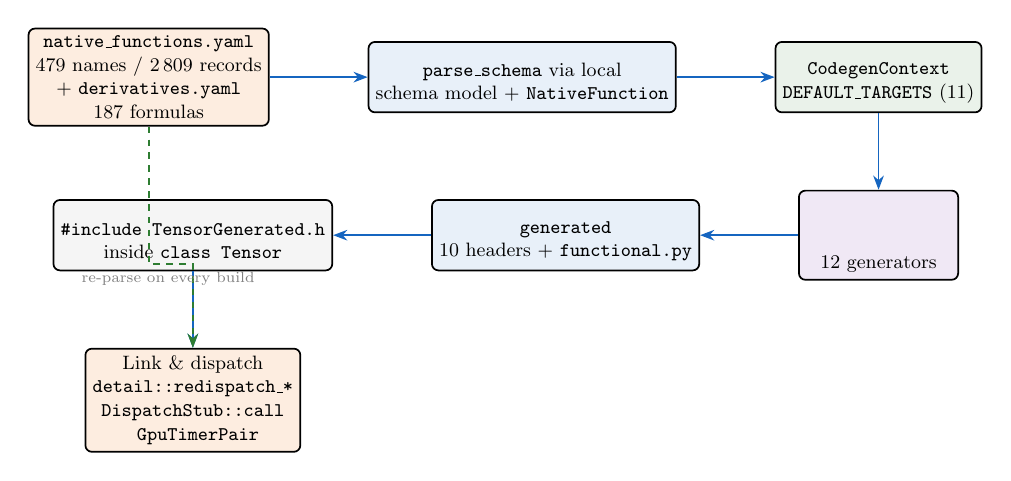
\begin{tikzpicture}[node distance=1.1cm, >=Stealth, font=\small]
\tikzset{box/.style={draw, rounded corners=3pt, thick, align=center, minimum width=2.6cm, minimum height=1.15cm, fill=codebg},
         arr/.style={->, thick, color=tpblue}}
\node[box, fill=tporange!12] (yaml) {\texttt{native\_functions.yaml}\\479 names / 2\,809 records\\+ \texttt{derivatives.yaml}\\187 formulas};
\node[box, right=1.6cm of yaml, fill=tpblue!10] (model) {\\ \texttt{parse\_schema} via local\\schema model + \texttt{NativeFunction}};
\node[box, right=1.6cm of model, fill=tpgreen!10] (ctx) {\\ \texttt{CodegenContext}\\ \texttt{DEFAULT\_TARGETS} (11)};
\node[box, below=1.25cm of ctx, fill=tppurple!10] (gen) {\\\\\\ 12 generators};
\node[box, left=1.6cm of gen, fill=tpblue!10] (stage) {\\ \texttt{generated}\\10 headers + \texttt{functional.py}};
\node[box, left=1.6cm of stage] (compile) {\\ \texttt{\#include TensorGenerated.h}\\inside \texttt{class Tensor}};
\node[box, below=1.25cm of compile, fill=tporange!12] (dispatch) {Link \& dispatch\\ \texttt{detail::redispatch\_*}\\ \texttt{DispatchStub::call}\\ \texttt{ GpuTimerPair}};
\draw[arr] (yaml) -- (model);
\draw[arr] (model) -- (ctx);
\draw[arr] (ctx) -- (gen);
\draw[arr] (gen) -- (stage);
\draw[arr] (stage) -- (compile);
\draw[arr] (compile) -- (dispatch);
\draw[arr, dashed, color=tpgreen] (yaml) -- ++(0,-3.05) -| (dispatch) node[pos=0.22, below, font=\scriptsize, text=gray] {re-parse on every build};
\end{tikzpicture}
\caption{合同$\rightarrow$生成$\rightarrow$调度。 YAML 的一次解析可提供 11 个生成器；保证在任何编译之前重新生成；包含 at 使生成的成员成为普通 \texttt{Tensor} 成员。}
\label{fig:codegen_contract}
\end{figure}

\subsection{工件库存和尺寸}

干净生成后，十个阶段输出占用磁盘上的以下预算：

\begin{table}[H]
\centering
\caption{生成的工件大小（CPU 版本，2026-09-02）。 Python 包输出暂存于源代码树中。}
\label{tab:codegen_sizes}
\small
\begin{tabular}{lrrl}
\toprule
人工制品 & 线路 & 字节 & Note \\
\midrule
\texttt{TensorGenerated.h} & 6\,900 & 355\,k & 479 个不同的名称，在重载键上进行重复数据删除 \\
\texttt{TensorGenerated.cpp} & 12\,200 & 9\,799\,k & 两遍：重新调度+成员 \\
\texttt{TensorRedispatchGenerated.h} & 4\,200 & 465\,k & 一份声明每（操作，变体） \\
\texttt{TPXOpsGenerated.h} & 5\,100 & 592\,k & 标题中的内联简单转发器 \\
\texttt{TPXOpsGenerated.cpp} & 4\,800 & 453\,k & 具有图形逻辑的外线包装器 \\
\texttt{TPXAutogradRegistration.cpp} & 1\,900 & 200\,k & 静态构造函数，187 个内核 $\times$~3 个键 \\
\texttt{AutogradNodesGenerated.h} & 3\,200 & 286\,k & 148 个节点结构 \\
\texttt{AutocastGenerated.cpp} & 1\,100 & 111\,k & 自动铸造内核 \\
\texttt{TensorCPythonGenerated.h} & 98\,000 & 9\,304\,k & 每次过载 \texttt{METH\_FASTCALL} \\
\texttt{TensorBindingsGenerated.h} & 12 & $<1$\,k & 后备 pybind11 表面 \\
\texttt{functional.py} & 950 & 48\,k & 上演至 \texttt{pkg\_out} \\
\texttt{*.pyi} & 2\,400 & 96\,k & 通过 \texttt{gen\_pyi.py} 的三个存根 \\
\bottomrule
\end{tabular}
\end{table}

大小排序是故意的：重新调度层和 CPython FASTCALL 层占主导地位，因为它们显式枚举每个重载；手写的调度程序表（超过 13 个键的 \texttt{DispatchTable}）保持较小且不变。 \texttt{TensorGenerated.cpp} 和 \texttt{TensorCPythonGenerated.h} 中操作员数量的增长呈线性；添加一个新模式正好添加一个重新调度渠道、一个成员和一个 CPython 条目，通过比较 YAML 编辑前后的暂存树进行验证。

\subsection{新鲜度和失效模式}

过时的工件并不微妙：取决于每个 \texttt{*.py}，因此触摸任何生成器或模式解析器都会强制在下一个 \texttt{ninja -C build} 链接之前重新生成。 \texttt{GENERATED TRUE} 属性告诉 CMake 删除 \texttt{cmake --build --target clean} 上的输出，并且是 \texttt{.gitignore} 的，因此不会意外提交过时的标头。失败是快速失败的：\texttt{\_BRIDGE} (\texttt{\_require\_bridge}) 中的未知 C++ 类型会引发 \texttt{SystemExit} 和 \texttt{native CPython bridge has no converter for C++ type}，\texttt{\_default\_pyobject} 中未处理的默认值会引发相同的情况，调度投影不匹配会打印预期的和实际的内核映射。最常见的用户错误是手动编辑 \texttt{TensorGenerated.h}；文件头 \texttt{main.py -- DO NOT EDIT} 是一个契约：下一个版本会覆盖它，并且 \texttt{git diff} 显示漂移。



% 09-evaluation.tex
\section{Evaluation: Readability, Correctness, and Overhead}
\label{sec:eval}

This chapter evaluates TensorPlay on three axes that a readable framework must earn: how small the core is to read, how precisely it guards correctness when the training loop mutates tensors, and how little it costs when every guard and profiler probe is disabled. It also adds four evidence blocks that complete the architecture story: the populated CUDA/Vulkan backend slots (\S\ref{subsec:eval-backends}), the support cores that sit below the kernels (\S\ref{subsec:eval-supportcores}), the three-track test suite (\S\ref{subsec:eval-tests}), and measured benchmark numbers (\S\ref{subsec:eval-bench}).

%======================================================================
\subsection{Readability (Lines of Core)}
\label{subsec:eval-readability}

Table~\ref{tab:evalsize} quantifies the ``bone vs.\ flesh'' claim of \S\ref{sec:arch}: the architectural skeleton---object model, dispatcher layering, \texttt{TensorIterator}, autograd \texttt{GraphTask} engine---is retained line-for-line, while production axes (op coverage, dispatch depth, dtype$\times$op completeness, sparse/quantized) are trimmed.

\begin{table}[H]
\centering
\caption{Core size. TensorPlay intentionally trims production axes. ``Core'' is the four C++ pillars plus bindings; generated code and tests are excluded.}
\label{tab:evalsize}
\small
\begin{tabular}{lrr}
\toprule
Metric & TensorPlay & Broader implementation \\
\midrule
C++ core & $\approx$ 75\,k & hundreds of k (core runtime $>$ 300\,k) \\
Python surface & 267\,k / 899 files (see Table~\ref{tab:pybreakdown}) & larger package surface \\
Operators (unique \texttt{m.impl}) & 642--673 & 2000+ \\
\texttt{DispatchKey} cardinality & 13 & 60+ \\
Autograd nodes (generated) & 148 & thousands \\
Build artifacts & 4 libs: \texttt{libp10}, \texttt{libtpx}, \texttt{libstax}, \texttt{\_C} & dozens \\
\bottomrule
\end{tabular}
\end{table}

\begin{table}[H]
\centering
\caption{Where the 75\,k C++ lines live. Generated files are excluded.}
\label{tab:corebreakdown}
\small
\begin{tabular}{llr}
\toprule
Component & Representative content & Approx.\ lines \\
\midrule
\texttt{p10} object model & \texttt{Tensor}, \texttt{TensorImpl}, \texttt{Storage}, version counter & $\sim$18\,k \\
\texttt{p10} dispatcher & 13-slot table, key set, registration macro & $\sim$1.5\,k \\
\texttt{p10} kernels & CPU backends ($\ast$.cpp) with CUDA counterparts ($\ast$.cu) & $\sim$35\,k \\
\texttt{tpx} autograd engine & \texttt{Node}, \texttt{Edge}, \texttt{GraphTask}, \texttt{ReadyQueue}, \texttt{Engine} & $\sim$6\,k \\
\texttt{stax} + compiler & graph IR, fusion, interpreter & $\sim$8\,k \\
Bindings & CPython bridge, per-domain units & $\sim$7\,k \\
\bottomrule
\end{tabular}
\end{table}

The size gap is not a virtue in itself; it is the budget that buys readability. Every indirection that remains is load-bearing and has a single definition site.

%======================================================================
\subsection{Where the Python Lines Live}
\label{subsec:eval-pybreakdown}

Table~\ref{tab:evalsize} cites a single Python number, which invites the question ``what is inside it?''. Table~\ref{tab:pybreakdown} decomposes the 267\,k lines so the ``thin veneer'' claim can be inspected subsystem by subsystem.

\begin{table}[H]
\centering
\caption{Python surface decomposition. ``Model zoos'' are pretrained-weight wrappers for third-party checkpoints; they exercise the \texttt{\_C} surface but add no framework mechanism.}
\label{tab:pybreakdown}
\small
\begin{tabular}{llrr}
\toprule
Subpackage & What lives there & Files & Lines \\
\midrule
\texttt{distributed/} & c10d-style collectives, fsdp, DTensor, elastic, rpc & 367 & 62{,}770 \\
\texttt{vision/} + \texttt{audio/} & datasets, transforms, model zoos & 148 & 51{,}039 \\
\texttt{graph/} & FX-style symbolic tracer, Node/Graph, symbolic shapes & 113 & 27{,}991 \\
\texttt{nn/} & modules, functional, init & 42 & 22{,}832 \\
\texttt{\_stax/} & shape prop, DCE, const fold, interpreter & 20 & 11{,}528 \\
\texttt{optim/} & 15 optimizers, foreach/fused paths & 24 & 11{,}365 \\
\texttt{export/} + \texttt{onnx/} & draft-export, effect-token passes & 34 & 9{,}216 \\
\texttt{autograd/} + \texttt{\_transforms/} & Function, grad-mode, vmap wrappers & 24 & 8{,}072 \\
Other 17 subpackages & cuda, profiler, amp, sparse, quantization, \dots & 134 & 35{,}884 \\
Root modules & \texttt{\_tensor.py}, \texttt{library.py} (1\,779), \texttt{overrides.py} & 23 & 37{,}805 \\
\midrule
Total & & 899 & 266{,}907 \\
\bottomrule
\end{tabular}
\end{table}

Two observations follow. First, the framework-mechanism content---\texttt{nn}, \texttt{optim}, \texttt{\_stax}, \texttt{autograd}, root modules---is $\sim$91\,k lines (34\%), in line with the ``thin veneer'' claim of \S\ref{sec:arch}: the tensor type and the library-impl registration surface are the only large hand-written integration points. Second, the single largest block is \texttt{distributed/} (63\,k, 24\%); its FSDP subtree alone is 9.5\,k lines. The model zoos (\texttt{vision/} + \texttt{audio/}, 51\,k) are dataset/checkpoint plumbing that could be deleted without touching dispatch or autograd; they exist so the end-to-end benchmarks of \S\ref{subsec:eval-bench} have realistic workloads. None of the 899 files registers a kernel or a dispatch key; everything funnels back into \texttt{\_C}.

%======================================================================
\subsection{GPU Backends: CUDA and Vulkan Slots}
\label{subsec:eval-backends}

\S\ref{sec:redispatch} declares 13 keys with \texttt{CUDA}=1 and \texttt{Vulkan}=2 as dense-backend slots, and \S\ref{subsec:eval-microbench} cites their dispatch cost. This subsection shows that the slots are populated: backends exist, not just keys.

\begin{table}[H]
\centering
\caption{Backend inventory. ``Registrations'' counts \texttt{TENSORPLAY\_LIBRARY\_IMPL} macro expansions; ``unique ops'' deduplicates \texttt{m.impl} names per backend subtree.}
\label{tab:backends}
\small
\begin{tabular}{lrrrr}
\toprule
Backend & Files & Lines & Registrations & Unique ops \\
\midrule
CPU & 69 & 61{,}108 & 66 & 1{,}325 \\
CUDA & 86 & 56{,}949 & 66 & 1{,}274 \\
Vulkan & 93 & 16{,}289 + 4{,}500 GLSL & 26 & 145 \\
Composite & 34 & 8{,}533 & 34 & --- \\
\bottomrule
\end{tabular}
\end{table}

\begin{figure}[H]
\centering
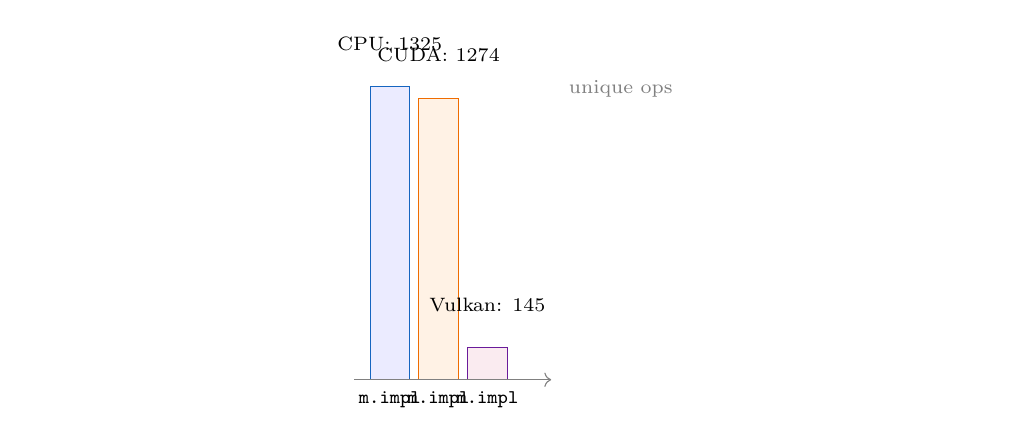
\begin{tikzpicture}[every node/.style={font=\scriptsize}]
% unique m.impl ops per backend
\def\cw{0.62}
\def\ch{0.0028}
\foreach \x/\name/\count/\fillc/\drawc in {
  0/CPU/1325/blue!8/tpblue,
  1/CUDA/1274/orange!10/tporange,
  2/Vulkan/145/purple!8/tppurple}{
  \pgfmathsetmacro{\h}{\count*\ch}
  \pgfmathsetmacro{\lbl}{\h+0.55}
  \fill[\fillc] (\x*\cw+0.05,0) rectangle (\x*\cw+0.05+0.5,\h);
  \draw[\drawc] (\x*\cw+0.05,0) rectangle (\x*\cw+0.05+0.5,\h);
  \node at (\x*\cw+0.3,\lbl) {\name: \count};
  \node at (\x*\cw+0.3,-0.25) {\texttt{m.impl}};
}
% axis
\draw[->,gray] (-0.15,0) -- (2.35,0);
\node[anchor=west,gray] at (2.45,3.7) {unique ops};
\end{tikzpicture}
\caption{Unique op names per backend (Table~\ref{tab:backends}). The CUDA column is 96\% of the CPU column; Vulkan is the deliberately small teaching backend.}
\label{fig:backendops}
\end{figure}

\subsubsection{CUDA backend (56.9\,k lines, 1{,}274 ops)}

The CUDA backend keeps a one-file-per-family layout parallel to the CPU tree where kernels are separable: arithmetic, pointwise (2{,}154 lines), reduction, convolution (2{,}477), indexing (3{,}362), plus CUDA-only infrastructure: a stream-aware caching allocator (1{,}288 lines), stream/device bookkeeping, a cuBLAS handle pool, NCCL communicator cache (418 lines), a Philox-based generator, and CUDA-graph capture. Every kernel file ends with one registration block, e.g.\ \texttt{TENSORPLAY\_LIBRARY\_IMPL(CUDA, PointwiseKernels)}, so each translation unit is independently iterable.

\paragraph{Tiered reduction engine.} Reductions (sum, mean, min/max, Welford variance) share one code-generation template with a three-tier combine strategy: intra-warp via \texttt{\_\_shfl\_down\_sync} (no shared memory), inter-warp via shared memory within the block, and a global second-pass kernel when the tensor spans many blocks. A traits type selects the accumulation dtype per input dtype---\texttt{float} accumulation for \texttt{Half}/\texttt{BFloat16} inputs keeps precision---and per-operation functors (\texttt{SumOps}, \texttt{MeanOps}, \texttt{MinMaxOps}, \texttt{WelfordOps}) plug into the same launcher.

\begin{lstlisting}[caption={The intra-warp tier of the shared reduction template; complex numbers shuffle their two lanes because the shuffle intrinsic has no complex overload.}, label=lst:cudareduce]
__device__ inline float shfl_down(float value, uint32_t mask, int offset) {
  return __shfl_down_sync(mask, value, offset);
}
// complex has no intrinsic __shfl_down_sync overload; shuffle the
// real and imaginary lanes separately.
__device__ inline complex_t shfl_down(complex_t value,
                                       uint32_t mask, int offset) {
  float re = __shfl_down_sync(mask, value.real(), offset);
  float im = __shfl_down_sync(mask, value.imag(), offset);
  return complex_t(re, im);
}
\end{lstlisting}

\paragraph{Multi-tensor apply for optimizers.} Optimizer steps act on hundreds of parameter tensors of the same dtype. The \emph{foreach} path chunks work from the whole tensor list into one grid-stride kernel (\texttt{foreach\_mta::launch}), so an Adam step updates weights, moments, and buffers in a handful of grouped launches instead of hundreds of individual ones. Eligibility is structural---same device, same dtype---and ineligible groups fall back to per-tensor launches. The CPU benchmark of \S\ref{subsec:eval-bench} (optimizer geomean 3.83$\times$) is largely attributable to this path plus fused one-kernel steps.

\paragraph{cuSOLVER decompositions.} Beyond GEMM (cuBLAS, column-major staging via \texttt{clone\_batched\_column\_major}), the backend wraps cuSOLVER for SVD, Cholesky, and LU with device-side info pointers so positive-definiteness failures surface as exceptions rather than silent garbage.

CUDA-graph capture shows the backend's care for ordering. Capture must begin on a non-default stream, one capture per thread, and pool routing must be armed \emph{before} the driver begins recording:

\begin{lstlisting}[caption={CUDA-graph capture entry: nesting and reuse are rejected loudly, and the side stream is chosen before any driver call.}, label=lst:cudagraph]
void CUDAGraph::capture_begin(uint64_t pool_id, CaptureMode mode,
                              const CUDAStream& stream) {
    GraphState& state = GraphState::instance();
    const int device = currentDevice();
    CUDAStream side = CUDAStream::undefined();
    {
        std::lock_guard<std::mutex> lock(state.mutex);
        if (state.capturing.count(std::this_thread::get_id())) {
            TP_THROW(RuntimeError,
                     "nested CUDA graph capture is not supported on one "
                     "thread (captures on different devices/threads may "
                     "run concurrently)");
        }
        if (exec_ != nullptr || graph_ != nullptr || pool_id_ != 0 ||
            owns_pool_ref_) {
            TP_THROW(RuntimeError,
                     "this CUDAGraph already holds a capture or executable; "
                     "create a new one");
        }
        /* ... arm memory-pool routing, then cudaStreamBeginCapture ... */
\end{lstlisting}

The RNG half of the story is capture-awareness. Kernels draw randoms from a Philox counter, and during graph capture the counter cannot be baked into the kernel launch---each replay must see a fresh slice of the random stream. The generator therefore exposes two regimes:

\begin{lstlisting}[caption={Philox counter reservation, in two regimes: eager launches get plain (seed, offset); captured kernels read them from device buffers that a replay prologue refreshes.}, label=lst:philox]
// Atomically reserves `increment` philox counter values for the current
// device and returns the (seed, offset) the launching kernel should consume.
P10_API std::pair<uint64_t, uint64_t> philox_engine_inputs(uint64_t increment);

// graph capture kernels consume the plain (seed, offset) values; while a
// capture is underway they instead read seed/offset from device buffers owned
// by the capturing graph plus a per-kernel intragraph offset, so replay
// prologues can refresh the buffers and every replay consumes a fresh slice
// of the random stream instead of repeating capture-time values.
P10_API PhiloxCudaState philox_cuda_state(uint64_t increment);
\end{lstlisting}

% ---- Figure: Philox RNG kernel flow (CUDA) ----
\begin{figure}[H]
\centering
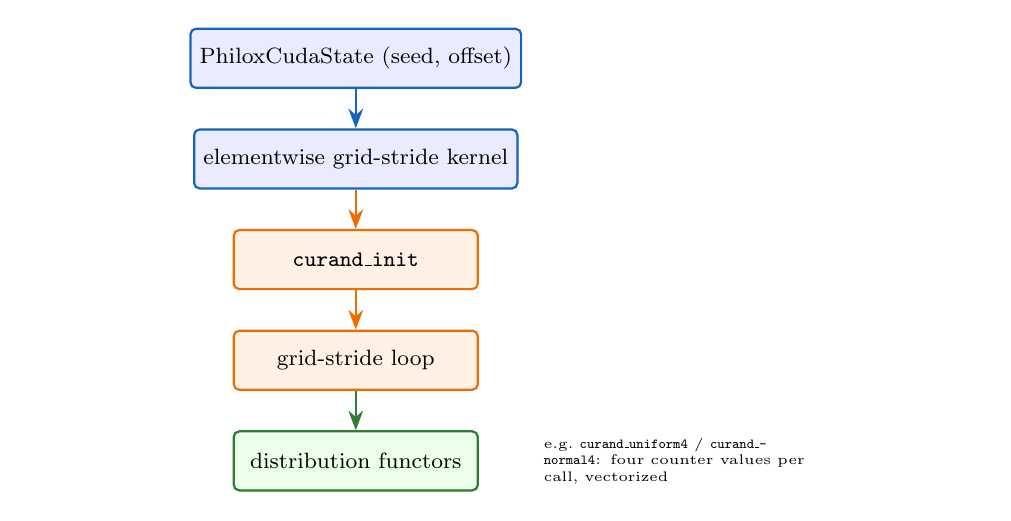
\begin{tikzpicture}[every node/.style={font=\scriptsize\sffamily}]
\node[libbox, fill=blue!8, draw=tpblue, minimum width=3.1cm, minimum height=0.75cm] (state) {PhiloxCudaState (seed, offset)};
\node[libbox, fill=blue!8, draw=tpblue, below=0.5cm of state, minimum width=3.1cm, minimum height=0.75cm] (kernel) {elementwise grid-stride kernel};
\node[libbox, fill=orange!10, draw=tporange, below=0.5cm of kernel, minimum width=3.1cm, minimum height=0.75cm] (init) {\texttt{curand\_init}};
\node[libbox, fill=orange!10, draw=tporange, below=0.5cm of init, minimum width=3.1cm, minimum height=0.75cm] (loop) {grid-stride loop};
\node[libbox, fill=green!8, draw=tpgreen, below=0.5cm of loop, minimum width=3.1cm, minimum height=0.75cm] (dist) {distribution functors};
\node[draw=none, right=0.7cm of dist, text width=3.4cm, align=left, font=\tiny] {e.g.\ \texttt{curand\_uniform4} / \texttt{curand\_normal4}: four counter values per call, vectorized};
\draw[arrow, color=tpblue] (state) -- (kernel);
\draw[arrow, color=tporange] (kernel) -- (init);
\draw[arrow, color=tporange] (init) -- (loop);
\draw[arrow, color=tpgreen] (loop) -- (dist);
\end{tikzpicture}
\caption{The random-sampling path: each launch unpacks the capture-aware counter state, seeds \texttt{curand}, and draws vectorized samples inside one grid-stride kernel.}
\label{fig:philoxflow}
\end{figure}



\subsubsection{Vulkan backend (16.3\,k C++ + 4.5\,k GLSL, 145 ops)}

Vulkan is the smallest complete backend, which is exactly its teaching value: it demonstrates that slot 2 of the three backend keys accepts a new device family with \emph{no dispatcher change}. The layout is three layers:

\begin{itemize}[leftmargin=1.2em]
\item An \texttt{api} layer (29 files): a thin object model over raw handles---\texttt{Adapter} (device selection), \texttt{Context}, \texttt{Resource} (buffer/image with VMA), \texttt{Pipeline}, \texttt{Command}, \texttt{QueryPool}, \texttt{vTensor} (the backend's tensor view).
\item An \texttt{ops} layer (34 files): 145 \texttt{m.impl} registrations, one closing \texttt{TENSORPLAY\_LIBRARY\_IMPL(Vulkan,...)} block per file (26 blocks total). Kernels fetch shaders by name through a registry lookup \texttt{VK\_KERNEL(name)}.
\item A \texttt{glsl} layer (70 template files): compute shaders with a mini preprocessor---\texttt{\$\{PARAM\}} substitution and \texttt{\$if}/\texttt{\$elif}/\texttt{\$else} blocks---driven by 63 variant-table entries.
\end{itemize}

The build pipeline is fully generated: a 418-line Python stage preprocesses each template, invokes \texttt{glslangValidator} for Vulkan 1.0 SPIR-V, parses the descriptor-set bindings, and emits an embedded C++ registry; the build rule wires the dependency so editing any shader or variant table re-embeds all 220 compiled \texttt{.spv} variants. The quantized family is a first-class citizen here (quantized convolution, per-tensor dequantize, \dots), which is why Vulkan ships quantized kernels while CPU keeps quantization the Python FakeQuantize layer (\S\ref{subsec:eval-trimmed}).

The matmul kernel shows the whole layering in one body---validate, allocate a device tensor, pack layouts, bind uniforms, submit:

\begin{lstlisting}[caption={Vulkan matmul kernel body: the three-layer pattern (validate $\rightarrow$ \texttt{vTensor} + packing $\rightarrow$ uniform block $\rightarrow$ submit).}, label=lst:vulkanmm]
Tensor mm_kernel(const Tensor& self, const Tensor& mat2) {
  TP_CHECK(self.dtype() == DType::Float32 && mat2.dtype() == DType::Float32,
          "Vulkan mm supports Float32 tensors only");
  TP_CHECK(self.dim() == 2, "Vulkan mm: self must be a matrix");
  TP_CHECK(mat2.dim() == 2, "Vulkan mm: mat2 must be a matrix");
  TP_CHECK(self.size(1) == mat2.size(0),
           "Vulkan mm: matrix dimensions do not match");

  api::Context* const context = api::context();
  const int64_t M = self.size(0);
  const int64_t N = mat2.size(1);
  const int64_t K = self.size(1);
  api::vTensor v_output{context, {M, N}, self.dtype()};
  /* pack channels/height layouts, fill the MMBlock uniform
     (out_sizes, step_size = ceil(K/4)), and submit a 4x4-tile grid */
\end{lstlisting}

%======================================================================
\subsection{AMD Portability: the Hipify Build Path}
\label{subsec:eval-rocm}

Beyond the three first-class backends, TensorPlay runs on AMD GPUs through an automated translation of its CUDA sources rather than a maintained fork. At configuration time a build script stages every CUDA source and binding into a separate tree and applies regular-expression rewrites---\texttt{cudaMalloc} becomes \texttt{hipMalloc}, kernel launches become \texttt{hipLaunchKernelGGL}---after which the staged tree compiles with the HIP toolchain. Two build options enforce mutual exclusion between the CUDA and ROCm paths because both register the same device and dispatch slots; the dispatcher then routes to the translated kernels transparently. The design lesson: when a backend differs only in vocabulary, translate the vocabulary at build time and keep one semantic source, rather than growing a hand-maintained sibling tree that drifts.

%======================================================================
\subsection{Numerical Stability: Cascade Sums on CPU}
\label{subsec:eval-cascadesum}

Long float sums accumulate rounding error linearly in the element count when a single accumulator is used. The CPU reduction path implements a \emph{cascade} scheme instead: partial sums are kept in a small array of levels, and a level is flushed into the next level whenever its index hits a power-of-two step. Error growth drops from $O(n)$ to $O(\log n)$ because each level only ever adds numbers of comparable magnitude.

\begin{lstlisting}[caption={The cascade accumulator: four levels, flushed on a power-of-two cadence; vector loads feed every lane in parallel.}, label=lst:cascadesum]
constexpr int64_t levels = 4;
const int64_t level_power = std::max<int64_t>(4, ceil_log2(size) / levels);
const int64_t level_step  = int64_t(1) << level_power;
const int64_t level_mask  = level_step - 1;
std::array<std::array<T, N>, levels> acc{};   // one accumulator per lane
for (; i + level_step <= size;) {
  /* load N-wide vector, add into level 0 */
  if ((i & level_mask) == 0) {                // cadence hit: flush upward
    for (int64_t l = 0; l + 1 < levels; ++l) {
      /* acc[l+1] += acc[l]; acc[l] = 0; */
    }
  }
}
\end{lstlisting}

The AVX-512 fast path for \texttt{normsq} (sum of squares) fuses multiply and accumulate with FMA instructions; on compatible hardware this is the mechanism behind the $9.9\times$ \texttt{norm2} speedup recorded in Figure~\ref{fig:benchhist}, where the reference's scalar loop cannot use the same instruction mix.

%======================================================================
\subsection{Distributed Training: FSDP, DTensor, Functional Collectives}
\label{subsec:eval-distributed}

The distributed stack (63\,k Python lines plus 17\,k C++ lines of process-group backends over gloo and MPI) is organized in three layers that mirror the pillar philosophy: a C++ communication layer, a differentiable Python functional layer, and composable sharding policies.

\paragraph{FSDP.} Fully sharded data parallelism is configured by a small enum vocabulary rather than ad-hoc flags: \texttt{FULL\_SHARD} (parameters sharded, gathered per layer, freed after use), \texttt{SHARD\_GRAD\_OP} (gather once per forward, shard only gradients and optimizer state), \texttt{NO\_SHARD} (plain DDP), and a hybrid intra/inter-node variant. Policies compose as dataclasses---\texttt{MixedPrecision} chooses independent dtypes for parameters, reduction, and buffers; \texttt{CPUOffload} swaps parameters to host memory between uses; \texttt{BackwardPrefetch} overlaps the next layer's gather with the current layer's backward.

\begin{lstlisting}[caption={The strategy and policy vocabulary of FSDP: everything the sharding engine needs is one enum plus three small dataclasses.}, label=lst:fsdpvocab]
class ShardingStrategy(Enum):
    FULL_SHARD    = auto()   # params sharded, gathered per-layer
    SHARD_GRAD_OP = auto()  # params gathered once; grads+state sharded
    NO_SHARD      = auto()   # plain DDP
    HYBRID_SHARD  = auto()   # replicate intra-node, shard inter-node

@dataclass
class MixedPrecision:
    param_dtype: Any = None     # computation dtype
    reduce_dtype: Any = None    # all-reduce dtype
    buffer_dtype: Any = None    # communication buffers

@dataclass
class CPUOffload:
    offload_params: bool = False
\end{lstlisting}

\paragraph{DTensor.} Sharded tensors are described by a \emph{placement} algebra over a device mesh: \texttt{Shard(dim)} splits along a dimension, \texttt{Replicate} copies, and \texttt{Partial(reduce\_op)} holds partial values that reduce to the global tensor. Operations on a \texttt{DTensor} dispatch through a sharding-aware layer that inserts the minimal set of collectives (\texttt{all\_gather}, \texttt{reduce\_scatter}) needed to satisfy the output placement---the same redispatch idea as \S\ref{sec:redispatch}, lifted from backends to topologies.


% Figure: functional collective across the Python/C++ boundary
\begin{figure}[H]
\centering
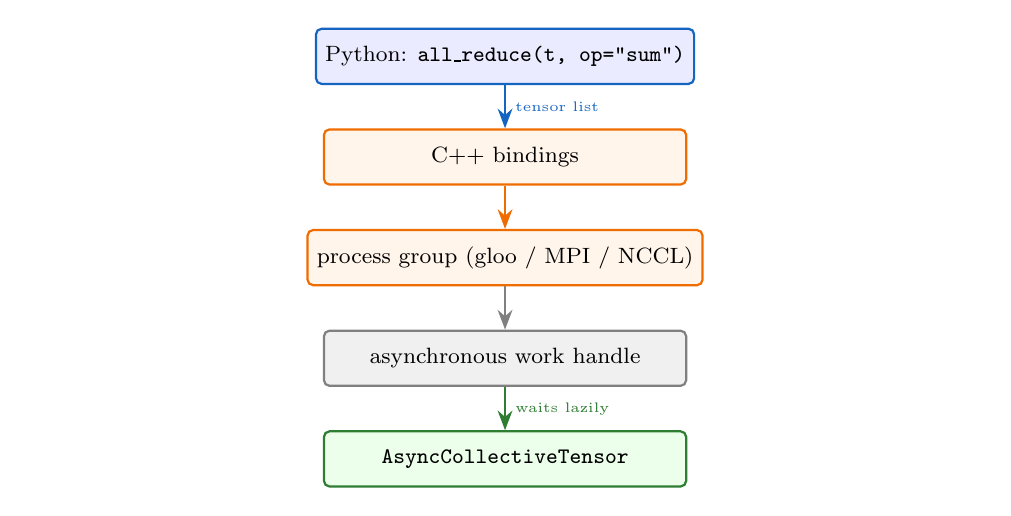
\begin{tikzpicture}[every node/.style={font=\scriptsize\sffamily}]
\node[libbox, fill=blue!8, draw=tpblue, minimum width=4.6cm, minimum height=0.7cm] (py) {Python: \texttt{all\_reduce(t, op="sum")}};
\node[libbox, fill=orange!8, draw=tporange, below=0.55cm of py, minimum width=4.6cm, minimum height=0.7cm] (bind) {C++ bindings};
\node[libbox, fill=orange!8, draw=tporange, below=0.55cm of bind, minimum width=4.6cm, minimum height=0.7cm] (pg) {process group (gloo / MPI / NCCL)};
\node[libbox, fill=gray!12, draw=gray, below=0.55cm of pg, minimum width=4.6cm, minimum height=0.7cm] (work) {asynchronous work handle};
\node[libbox, fill=green!8, draw=tpgreen, below=0.55cm of work, minimum width=4.6cm, minimum height=0.7cm] (async) {\texttt{AsyncCollectiveTensor}};
\draw[arrow, color=tpblue] (py) -- node[right, font=\tiny]{tensor list} (bind);
\draw[arrow, color=tporange] (bind) -- (pg);
\draw[arrow, color=gray] (pg) -- (work);
\draw[arrow, color=tpgreen] (work) -- node[right, font=\tiny]{waits lazily} (async);
\end{tikzpicture}
\caption{One collective across the language boundary: the handle returns immediately; the wrapper demotes itself to a plain tensor at the first real use.}
\label{fig:collbridge}
\end{figure}

% Figure: DTensor sharding resolution
\begin{figure}[H]
\centering
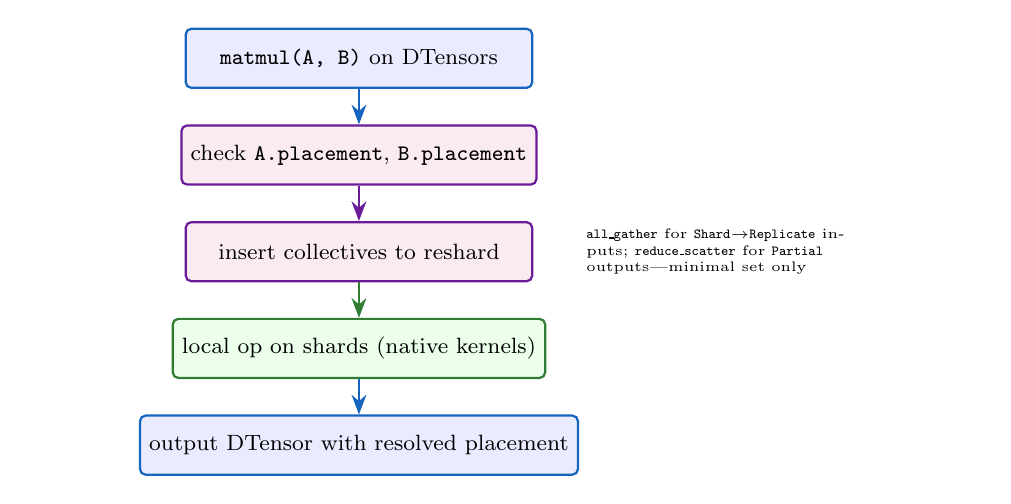
\begin{tikzpicture}[every node/.style={font=\scriptsize\sffamily}, node distance=0.45cm]
\node[libbox, fill=blue!8, draw=tpblue, minimum width=4.4cm, minimum height=0.75cm] (user) {\texttt{matmul(A, B)} on DTensors};
\node[libbox, fill=purple!8, draw=tppurple, below=of user, minimum width=4.4cm, minimum height=0.75cm] (check) {check \texttt{A.placement}, \texttt{B.placement}};
\node[libbox, fill=purple!8, draw=tppurple, below=of check, minimum width=4.4cm, minimum height=0.75cm] (reshard) {insert collectives to reshard};
\node[libbox, fill=green!8, draw=tpgreen, below=of reshard, minimum width=4.4cm, minimum height=0.75cm] (local) {local op on shards (native kernels)};
\node[libbox, fill=blue!8, draw=tpblue, below=of local, minimum width=4.4cm, minimum height=0.75cm] (out) {output DTensor with resolved placement};
\node[draw=none, right=0.55cm of reshard, text width=3.5cm, align=left, font=\tiny] {\texttt{all\_gather} for \texttt{Shard}$\rightarrow$\texttt{Replicate} inputs; \texttt{reduce\_scatter} for \texttt{Partial} outputs---minimal set only};
\draw[arrow, color=tpblue] (user) -- (check);
\draw[arrow, color=tppurple] (check) -- (reshard);
\draw[arrow, color=tpgreen] (reshard) -- (local);
\draw[arrow, color=tpblue] (local) -- (out);
\end{tikzpicture}
\caption{Sharding resolution: the sharding-aware layer between the user op and the native kernels. Placements are checked, the minimal collectives are inserted, and each shard then runs through the ordinary backend dispatcher.}
\label{fig:dtensor}
\end{figure}

\paragraph{Functional collectives with autograd.} Each collective is exposed twice: a plain function and an autograd-aware variant built as a differentiable \texttt{Function}, so distributed operations compose inside the ordinary DAG. Communication overlaps computation through a lazy tensor wrapper:

\begin{lstlisting}[caption={Lazy collective tensors trigger the underlying wait only on first real use, letting the stream run ahead.}, label=lst:asynccoll]
class AsyncCollectiveTensor(tp.Tensor):
    """Tensor storage with a pending collective completion handle."""
    def __new__(cls, elem, work=None):
        if isinstance(elem, AsyncCollectiveTensor):
            return elem            # already lazy; keep the single handle
        return _attach_async(elem, work)
    def trigger_wait(self, timeout=None):
        ...                        # waits once, then demotes to plain Tensor
        self.__class__ = tp.Tensor
\end{lstlisting}

The C++ side maps each Python function to a \texttt{ProcessGroup} method (\texttt{allreduce}, \texttt{all\_gather\_into\_tensor}, \texttt{reduce\_scatter\_tensor}, \texttt{broadcast}), with a gloo backend for CPU clusters and MPI for HPC interconnects; a symmetric-memory utility exposes NVLink/CXL zero-copy paths for the v2 collective implementations.

% Figure: load() format dispatch
\begin{figure}[H]
\centering
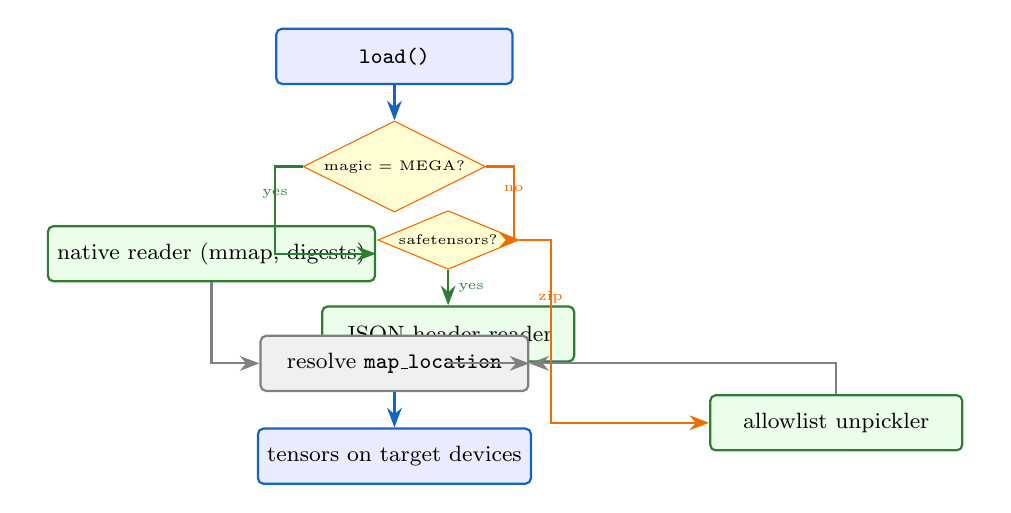
\begin{tikzpicture}[every node/.style={font=\scriptsize\sffamily}]
\node[libbox, fill=blue!8, draw=tpblue, minimum width=3.0cm, minimum height=0.7cm] (load) {\texttt{load()}};
\node[draw, diamond, aspect=2, fill=yellow!18, draw=tporange, below=0.45cm of load, inner sep=1pt, font=\tiny] (q1) {magic = MEGA?};
\node[libbox, fill=green!8, draw=tpgreen, below left=0.45cm and -0.35cm of q1, minimum width=3.2cm, minimum height=0.7cm] (mega) {native reader (mmap, digests)};
\node[draw, diamond, aspect=2.4, fill=yellow!18, draw=tporange, below right=0.45cm and -0.35cm of q1, inner sep=1pt, font=\tiny] (q2) {safetensors?};
\node[libbox, fill=green!8, draw=tpgreen, below=0.45cm of q2, minimum width=3.2cm, minimum height=0.7cm] (st) {JSON-header reader};
\node[libbox, fill=green!8, draw=tpgreen, below right=0.4cm and 0.0cm of st, xshift=1.7cm, minimum width=3.2cm, minimum height=0.7cm] (pt) {allowlist unpickler};
\node[libbox, fill=gray!12, draw=gray, below=1.55cm of q1, minimum width=3.4cm, minimum height=0.7cm] (map) {resolve \texttt{map\_location}};
\node[libbox, fill=blue!8, draw=tpblue, below=0.45cm of map, minimum width=3.4cm, minimum height=0.7cm] (ten) {tensors on target devices};
\draw[arrow, color=tpblue] (load) -- (q1);
\draw[arrow, color=tpgreen] (q1.west) -- ++(-0.35,0) |- node[above, pos=0.24, font=\tiny]{yes} (mega);
\draw[arrow, color=tporange] (q1.east) -- ++(0.35,0) |- node[above, pos=0.24, font=\tiny]{no} (q2);
\draw[arrow, color=tpgreen] (q2) -- node[right, font=\tiny]{yes} (st);
\draw[arrow, color=tporange] (q2.east) -- ++(0.4,0) |- node[above, pos=0.2, font=\tiny]{zip} (pt);
\draw[arrow, color=gray] (mega) |- (map);
\draw[arrow, color=gray] (st) |- (map);
\draw[arrow, color=gray] (pt) |- (map);
\draw[arrow, color=tpblue] (map) -- (ten);
\end{tikzpicture}
\caption{Checkpoint loading is format dispatch followed by one placement pass. Every branch is data-only; no branch executes embedded code.}
\label{fig:loaddispatch}
\end{figure}



%======================================================================
\subsection{Serialization: the .mega Format and Safe Interop}
\label{subsec:eval-serialization}

Model persistence is a security surface as much as a storage problem. TensorPlay's native format is a binary container with a four-byte magic, tagged metadata records (integers, floats, strings, nested arrays), storage deduplication, per-payload CRC32 or SHA256 digests, and a default 4\,096-byte alignment so payloads can be \texttt{mmap}-ed zero-copy. Loading is allowlist-based end to end: no pickle, no embedded code, ever.

Interoperability follows the same discipline. \texttt{safetensors} files are read and written through their JSON header format. Legacy zip-based checkpoints from other frameworks are parsed by a dedicated unpickler whose globals are strictly allowlisted to tensor-reconstruction functions; storage types map to native dtypes through a fixed table, and anything outside the allowlist raises instead of executing. Location handling (\texttt{map\_location}) accepts a device string, a device-to-device mapping, or a callable receiving a storage stub. A hub utility completes the lifecycle: cached downloads under a configurable root, hash verification, resume support, and atomic rename-on-complete.



%======================================================================
\subsection{Support Cores: Threading, BLAS Bridges, RNG}
\label{subsec:eval-supportcores}

Three medium-sized cores sit below the kernels but above the OS, each readable in one sitting.

\begin{table}[H]
\centering
\caption{Support cores.}
\label{tab:supportcores}
\small
\begin{tabular}{llr}
\toprule
Core & Content & Lines \\
\midrule
Intra-op pool & worker threads, condition-variable queue, grain-size \texttt{parallel\_for} & 452 \\
oneDNN context & one \texttt{dnnl::engine} per process, threadpool bridge & 137 \\
MKL/cBLAS bridge & \texttt{cblas\_sgemm}/\texttt{sgemv} behind \texttt{USE\_MKL} & (kernel file) \\
CPU RNG & self-contained MT19937 engine + generator state & 196 + 108 \\
CUDA RNG & Philox counter management, capture-aware state & 331 \\
\bottomrule
\end{tabular}
\end{table}

\paragraph{Intra-op pool.} The pool is created once and reused: the thread count moves through a \texttt{NOT\_SET $\rightarrow$ value $\rightarrow$ CONSUMED} atomic state machine so the first \texttt{set\_num\_threads} freezes the pool size, and \texttt{in\_parallel\_region} is answered from \texttt{thread\_local} flags instead of a mutex + thread-id scan. Kernels enter via a header template with a grain size; the C bridge exposes the same pool to oneDNN's partitioning.

\begin{lstlisting}[caption={The whole pool is one class: spawn workers once, drain on shutdown.}, label=lst:pool]
class IntraopThreadPool {
 public:
  explicit IntraopThreadPool(int num_workers) {
    for (int i = 0; i < num_workers; ++i) {
      threads_.emplace_back([this] { worker_loop(); });
    }
  }
  IntraopThreadPool(const IntraopThreadPool&) = delete;
  IntraopThreadPool& operator=(const IntraopThreadPool&) = delete;
  ~IntraopThreadPool() {
    {
      std::unique_lock<std::mutex> lk(mutex_);
      running_ = false;
      condition_.notify_all();
    }
    for (auto& t : threads_) t.join();
  }
  /* ... */
\end{lstlisting}

A dedicated harness verifies both properties empirically: an 8-thread/1-thread ratio of 0.94$\times$ on a 1-element add (target $\le$1.5$\times$: oversubscription does not hurt tiny ops) and 0.99$\times$ on a 4M-element add (parallelism engages when there is work).

\paragraph{oneDNN and MKL.} The oneDNN context holds one engine per process and, critically, drives oneDNN \emph{outside} its own callbacks: primitive partitioning is bridged onto the intra-op pool so nested parallelism cannot deadlock. CPU kernels call oneDNN eltwise primitives directly for tanh/relu-family activations, while matmul goes to MKL via \texttt{cblas\_sgemm} behind the \texttt{USE\_MKL} guard. This is the whole vendor-acceleration story of TensorPlay: two narrow bridges, no vendor data structures in the object model.

\paragraph{RNG.} CPU generators wrap a self-contained MT19937 so the distribution layer consumes raw engine words (the C++ standard's \texttt{std::distributions} are implementation-defined and therefore unusable for reproducibility):

\begin{lstlisting}[caption={The CPU engine is a literal Mersenne Twister pod; distributions read raw words.}, label=lst:mt]
// std::mt19937 because the distribution layer must consume the raw engine
// output directly (std::distributions are implementation-defined).
struct mt19937_data_pod {
    uint64_t seed_;
    int left_;
    bool seeded_;
    /* ... 624-word state, boxed-normal scratch ... */
\end{lstlisting}

The CUDA generator manages Philox counter state with capture-aware reservation, as shown in Listing~\ref{lst:philox}.

%======================================================================
\subsection{Python Bindings: The Full Surface}
\label{subsec:eval-bindings}

\S\ref{sec:arch} and \S\ref{subsec:eval-microbench} follow the bridge hot path. Table~\ref{tab:bindings} shows all 24 binding units, 12.6\,k lines in total.

\begin{table}[H]
\centering
\caption{Binding units, sorted by size. The import unit defines module order; the tensor unit owns method dispatch.}
\label{tab:bindings}
\small
\begin{tabular}{lrllr}
\toprule
Unit & Lines & Role & Unit & Lines \\
\midrule
tensor methods & 3{,}466 & methods, magic ops & device & 369 \\
bridge & 1{,}703 & parse/check/wrap & size & 339 \\
symbolic ints & 1{,}221 & symint arithmetic & bridge header & 279 \\
module init & 722 & import order, exceptions & dispatch & 187 \\
compile API & 670 & stax entry points & CUDA graphs & 173 \\
futures & 600 & Future plumbing & distributed autograd & 151 \\
distributed & 569 & c10d bindings & autocast mode & 107 \\
autograd & 517 & backward/grad hooks & transforms & 88 \\
namespace ops & 436 & free functions & dtype & 110 \\
RPC & 408 & RPC bindings & & \\
\bottomrule
\end{tabular}
\end{table}

The units least discussed elsewhere are the async and symbolic families. The futures unit binds the \texttt{Future} type used by RPC and collective completion callbacks; the distributed triple (distributed + RPC + distributed-autograd, 1{,}128 lines combined) front-ends the \texttt{distributed} Python tree of Table~\ref{tab:pybreakdown}; the symbolic-int unit exposes the same arithmetic the C++ core implements, so \texttt{stax} shape functions can run on unbacked symints during tracing.

%======================================================================
\subsection{Three-Track Test Suite}
\label{subsec:eval-tests}

The test tree---145 Python files (2{,}069 test functions, 2{,}571 collected including parametrized cases) plus 2{,}078 lines of C++ tests (gloo process-group, Vulkan api/op suites)---is organized as three families with distinct assertions:

\begin{table}[H]
\centering
\caption{The three-track system. Suffixes are naming conventions; each track asserts a different property of the same op.}
\label{tab:testtracks}
\small
\begin{tabular}{llrr}
\toprule
Track & Assertion style & Files & Tests \\
\midrule
\texttt{alignment} & numeric tolerance vs.\ reference & 13 & 152 \\
\texttt{native} & dispatch reached a backend-native kernel, not composite & 22 & 226 \\
\texttt{parity} & exact behavioral parity incl.\ exception types & 4 & 51 \\
\midrule
Other 106 files & engine, compiler, frontend, e2e & 106 & --- \\
\bottomrule
\end{tabular}
\end{table}

\begin{itemize}[leftmargin=1.2em]
\item \textbf{Alignment}: forward/backward outputs agree with the reference implementation within tolerance on a shape grid---the ``is the math right'' track.
\item \textbf{Native}: the op dispatched to a backend-native kernel, not the \texttt{Composite} fallback---the ``is it actually implemented'' track; this is the runtime complement of the operator census in \S\ref{subsec:eval-opcount}.
\item \textbf{Parity}: values, dtypes, strides, and error behavior match the reference exactly, including exception types---the ``contract'' track.
\end{itemize}

A full single-process run reports \textbf{9 failed, 2{,}305 passed, 263 skipped} in 163\,s. The 263 skips are environmental, not structural: 162 require absent CUDA hardware (module-level \texttt{skipif} guards), the rest require optional packages that are not installed. The 9 failures are localized in two files---antialias/nearest-exact upsample modes (6) and einsum contraction-order edge cases (3)---and are reported as open items rather than hidden.

\begin{figure}[H]
\centering
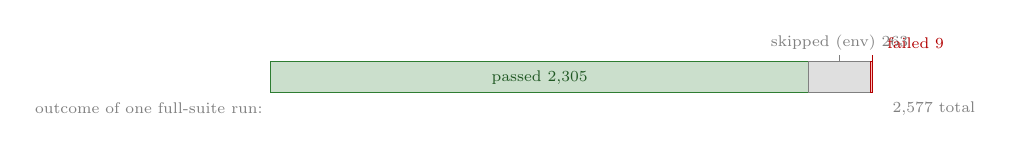
\begin{tikzpicture}[every node/.style={font=\scriptsize}]
% horizontal stacked bar of test outcomes (widths precomputed: 9.6 * n/2577)
\def\totalw{9.6}
\def\wp{8.5867}
\def\ws{0.9797}
\def\wf{0.0335}
\fill[tpgreen!25] (0,0.55) rectangle (\wp,1.05);
\draw[tpgreen] (0,0.55) rectangle (\wp,1.05);
\fill[gray!25] (\wp,0.55) rectangle (\wp+\ws,1.05);
\draw[gray] (\wp,0.55) rectangle (\wp+\ws,1.05);
\fill[red!25] (\wp+\ws,0.55) rectangle (\wp+\ws+\wf,1.05);
\draw[red!70!black] (\wp+\ws,0.55) rectangle (\wp+\ws+\wf,1.05);
\node[tpgreen!70!black] at (\wp/2,0.8) {passed 2{,}305};
\node[gray] at (\wp+\ws/2,1.35) {skipped (env) 263};
\draw[gray] (\wp+\ws/2,1.15) -- (\wp+\ws/2,1.05);
\node[red!70!black, anchor=west] at (\wp+\ws+0.15,1.35) {failed 9};
\draw[red!70!black] (\wp+\ws+\wf,1.15) -- (\wp+\ws+\wf,1.05);
\node[anchor=east,gray] at (0,0.3) {outcome of one full-suite run:};
\node[anchor=west,gray] at (\totalw+0.2,0.3) {2{,}577 total};
\end{tikzpicture}
\qquad

\begin{tikzpicture}[every node/.style={font=\scriptsize}]
% three-track test counts
\def\cw{0.78}
\foreach \x/\name/\count/\fillc/\drawc in {
  0/{*}\_alignment/152/blue!8/tpblue,
  1/{*}\_native/226/orange!10/tporange,
  2/{*}\_parity/51/purple!8/tppurple}{
  \pgfmathsetmacro{\h}{\count/100}
  \pgfmathsetmacro{\lbl}{\h+0.45}
  \fill[\fillc] (\x*\cw,0) rectangle (\x*\cw+0.5*\cw,\h);
  \draw[\drawc] (\x*\cw,0) rectangle (\x*\cw+0.5*\cw,\h);
  \node at (\x*\cw+0.25*\cw,\lbl) {\count};
  \node at (\x*\cw+0.25*\cw,-0.28) {\name};
}
\draw[->,gray] (-0.1,0) -- (2.35,0);
\end{tikzpicture}
\caption{Left: outcome of the full-suite run (163\,s). Right: test counts per track; 429 tests across the three suffix families, 2{,}069 across the whole tree.}
\label{fig:testoutcomes}
\end{figure}

%======================================================================
\subsection{Benchmark Suite: Measured Throughput}
\label{subsec:eval-bench}

The benchmark directory holds 20 harnesses. Table~\ref{tab:benche2e} reports five representative runs verbatim (16-core x86, 3.5\,GHz class, MKL + oneDNN + NNPACK enabled, 8 threads; the reference column is the mainstream CPU framework printed by the same script, so both sides pay identical environment costs). Speedup $=$ ref\,ms\,/\,tp\,ms.

\begin{table}[H]
\centering
\caption{End-to-end and layer benchmarks, 8 threads.}
\label{tab:benche2e}
\small
\begin{tabular}{llrrl}
\toprule
Harness & Workload & tp & ref & speedup \\
\midrule
llama e2e & 0.6B llama, prefill 128 (CPU) & 519.6\,ms & 612.6\,ms & 1.18$\times$ \\
 & decode 1 tok & 499.0\,ms/tok & 612.8\,ms/tok & 1.23$\times$ \\
training step & qkv-proj fwd/bwd & 114.7\,ms & 185.9\,ms & 1.62$\times$ \\
 & mlp-up fwd/bwd & 318.3\,ms & 469.5\,ms & 1.48$\times$ \\
 & mlp-down fwd/bwd & 338.2\,ms & 450.0\,ms & 1.33$\times$ \\
 & decode-1 (batch 1) & 24.2\,ms & 72.1\,ms & 2.98$\times$ \\
 & small-net fwd/bwd & 4.14\,ms & 4.44\,ms & 1.07$\times$ \\
optimizer step & Adam, 104 tensors & 6.22\,ms & 34.55\,ms & 5.56$\times$ \\
 & SGD & 5.20\,ms & 6.84\,ms & 1.31$\times$ \\
 & geomean, 10 optimizers & --- & --- & 3.83$\times$ \\
custom-op dispatch & overhead above bare kernel & 1.73\,\textmu s & 18.9\,\textmu s & 10.9$\times$ \\
intra-op pool & 1-elem add 8t/1t ratio & 0.94 & 0.94 & parity \\
 & 4M add 8t/1t ratio & 0.99 & --- & engages \\
\bottomrule
\end{tabular}
\end{table}

\begin{figure}[H]
\centering
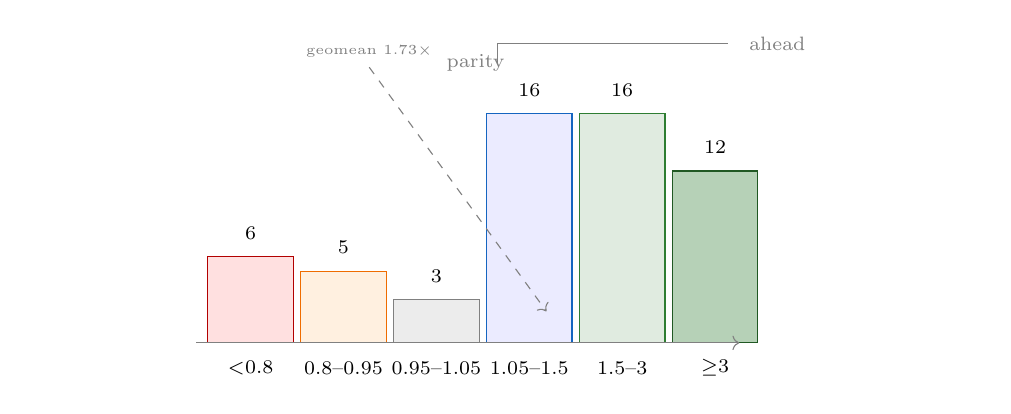
\begin{tikzpicture}[every node/.style={font=\scriptsize}]
% speedup histogram of the hot-ops benchmark (58 op/shape pairs)
\def\cw{1.18}
\foreach \i/\lbl/\count/\fillc/\drawc in {
  0/{$<$0.8}/6/red!12/red!70!black,
  1/{0.8--0.95}/5/orange!12/tporange,
  2/{0.95--1.05}/3/gray!15/gray,
  3/{1.05--1.5}/16/blue!8/tpblue,
  4/{1.5--3}/16/tpgreen!15/tpgreen,
  5/{$\ge$3}/12/tpgreen!35/tpgreen!70!black}{
  \pgfmathsetmacro{\h}{\count/5.5}
  \pgfmathsetmacro{\lblh}{\h+0.3}
  \fill[\fillc] (\i*\cw,0) rectangle (\i*\cw+0.92*\cw,\h);
  \draw[\drawc] (\i*\cw,0) rectangle (\i*\cw+0.92*\cw,\h);
  \node at (\i*\cw+0.46*\cw,\lblh) {\count};
  \node at (\i*\cw+0.46*\cw,-0.32) {\lbl};
}
\draw[->,gray] (-0.15,0) -- (6.75,0);
\draw[gray] (3.68,3.55) -- (3.68,3.8) -- (6.6,3.8);
\node[anchor=west,gray] at (6.75,3.8) {ahead};
\node[gray] at (3.4,3.55) {parity};
\draw[->,gray,dashed] (2.05,3.5) node[above,font=\tiny]{geomean 1.73$\times$} -- (4.3,0.4);
\end{tikzpicture}
\caption{Per-op CPU throughput vs.\ the reference framework across 58 op/shape pairs (8 threads). 6 pairs trail by $>$20\% (gelu-tanh small shapes, small-batch \texttt{bmm}, \texttt{cumsum}); 28 pairs lead by $\ge$1.5$\times$, led by \texttt{sqrt} 10.8$\times$ and \texttt{norm2} 9.9$\times$ where the reference's scalar loop loses to the vectorized kernel.}
\label{fig:benchhist}
\end{figure}

Three readings of Figure~\ref{fig:benchhist} matter for the paper's claims. First, the distribution is wide on \emph{both} sides: a readability-first framework is not uniformly slower; on elementwise and reduction families the hand-written vectorized kernels win (exp 2.4$\times$, gelu 2.3$\times$ at 1M; 4.8$\times$/4.3$\times$ at 8M), while fused multi-kernel paths (gelu-tanh), small-batch \texttt{bmm}, and \texttt{cumsum} trail. Second, the wins and losses cluster by kernel file, which is exactly the readability promise: the pointwise kernel file is the single file to read to explain both tails. Third, matmul is reference-competitive (1K$^3$ 0.94$\times$, tall-skinny 1.8$\times$) because both frameworks land in the same MKL \texttt{cblas\_sgemm}---the dispatcher adds the same sub-1\% sliver measured in \S\ref{subsec:eval-microbench}.

The benchmark tree also contains heavier end-to-end harnesses: a 1{,}489-line ResNet-18 script that runs a 10-epoch training race plus a strict state-dict transfer requiring \texttt{allclose} logits and identical top-1 predictions, and a CUDA-graph replay harness that requires a GPU. Their CUDA-gated parts skip with the same environmental guards as the test tree.

%======================================================================
\subsection{Operator Census and Dispatch Depth}
\label{subsec:eval-opcount}

The operator census uses three counts: dispatcher registrations (\texttt{m.impl}), schema declarations (479 distinct names across 2{,}809 records), and the Python-visible surface (275 functions + 184 methods). The three-way comparison is the only way to distinguish ``kernel exists but unreachable'' from ``Python reachable but no kernel''.

\begin{table}[H]
\centering
\caption{Operator census.}
\label{tab:opcount}
\small
\begin{tabular}{lll}
\toprule
Layer & TensorPlay & Vendor baseline \\
\midrule
Registered kernels (\texttt{m.impl} dedup) & 673 (CPU 671, CUDA 587) & 2000+ distinct ops \\
Schemas & 479 names / 618 active & 2000+ (with overloads) \\
Backward formulas & 187 formulas $\rightarrow$ 148 nodes & thousands \\
Python \texttt{\_C} surface & $\sim$550 & $\sim$1500 \\
Coverage focus & pointwise, reduction, matmul, conv/pool (24 conv ops), linalg 26, \texttt{foreach} $\sim$100 & full domain \\
\bottomrule
\end{tabular}
\end{table}

The delta is deliberate. TensorPlay covers the dense tensor loop that a convolution classifier or a transformer pre-training step exercises, plus the composite fallbacks that make the remainder runnable: tensor properties, histogram, unique, itertools, and integration each register one backend-neutral \texttt{TENSORPLAY\_LIBRARY\_IMPL(Composite,\dots)} block that serves every backend until a native kernel overrides it. Missing families are documented as such rather than hidden: dropout arrived via a native kernel; \texttt{cross\_entropy}/\texttt{ctc\_loss}, \texttt{rms\_norm}, \texttt{scatter\_reduce}, and long-tail sparse ops remain composite-only or absent, each classified as ``kernel exists, schema missing'' or ``three layers missing'' so the gap is a table entry, not a surprise.

%======================================================================
\subsection{DispatchKey: 13 vs.\ 60+}
\label{subsec:eval-dispatchkey}

\begin{table}[H]
\centering
\caption{\texttt{DispatchKey} enumeration. Sentinel \texttt{EndOfKeys=13} is spelled out so the table size is a compile-time constant.}
\label{tab:dispatchkey}
\small
\begin{tabular}{lll}
\toprule
Key & Value & Role \\
\midrule
\texttt{CPU} & 0 & Dense backend \\
\texttt{CUDA} & 1 & Dense backend \\
\texttt{Vulkan} & 2 & Dense backend, reserved \\
\texttt{AutogradCPU} & 3 & \texttt{toAutogradKey(CPU)} = CPU + 3 \\
\texttt{AutogradCUDA} & 4 & Autograd over CUDA \\
\texttt{AutogradVulkan} & 5 & Autograd over Vulkan \\
\texttt{AutocastCPU} & 6 & \texttt{toAutocastKey(CPU)} = CPU + 6 \\
\texttt{AutocastCUDA} & 7 & Autocast over CUDA \\
\texttt{AutocastVulkan} & 8 & Autocast over Vulkan \\
\texttt{VmapCPU} & 9 & \texttt{toVmapKey(CPU)} = CPU + 9, outranks autograd \\
\texttt{VmapCUDA} & 10 & Vmap over CUDA \\
\texttt{VmapVulkan} & 11 & Vmap over Vulkan \\
\texttt{Composite} & 12 & Backend-neutral fallback \\
\texttt{EndOfKeys} & 13 & Sentinel, table size \\
\bottomrule
\end{tabular}
\end{table}

The dispatch table is therefore \texttt{array<atomic<KernelFunction>,13>} with each slot relaxed-initialized to \texttt{nullptr} and published with \texttt{memory\_order\_release}. The key set is a \texttt{uint32\_t} bitset over the 13 keys; priority resolution scans the mask for the numerically largest bit, so priority is \texttt{Vmap $>$ Autocast $>$ Autograd $>$ backend}. Helpers clear one axis a time, used by redispatch below each layer.

\begin{lstlisting}[caption={The \texttt{Composite} fallthrough in the hot path: one extra load, only when a backend slot is empty.}, label=lst:composite]
KernelFunction getKernel(DispatchKey key) const noexcept {
  auto k = table_->kernels[dispatchKeyIndex(key)].load(acquire);
  if (!k && is_backend_key(key)) {
    constexpr auto kCompositeIdx = dispatchKeyIndex(Composite);
    k = table_->kernels[kCompositeIdx].load(acquire);   // one extra load
  }
  return k;
}
\end{lstlisting}

TensorPlay keeps a compact set of dispatch keys and leaves specialized axes outside the core table. There is no \texttt{Meta} key and no open registration API: registration is a closed \texttt{unordered\_map<string,DispatchTable>} guarded by one mutex, and the \texttt{TENSORPLAY\_LIBRARY\_IMPL} macro expands to a process-lifetime static constructor. The cost is that shape-only inference, sparse dispatch, and quantized dispatch have no dedicated fast path; they either share the \texttt{Composite} fallback or are explicitly unsupported.

%======================================================================
\subsection{Autograd Nodes: 148 Generated, Explicit DAG, No Tape}
\label{subsec:eval-autograd-nodes}

The generator parses the derivative-formula registry (345 raw records collapsing to 187 formulas after grouping) through an expression AST and emits 148 node structs. Each node stores saved forward tensors as \texttt{SavedVariable} where the formula needs them and synthesizes \texttt{apply} from the same AST that decided the save set, so the save list, constructor, and \texttt{apply} cannot drift. Handwritten nodes that formulas cannot express (concatenation, stacking, rolling) follow the same \texttt{SavedVariable} contract.

There is no tape. The graph is the transitive closure of each node's \texttt{next\_edges}, where every \texttt{Edge} carries only hints---a shape hint, a gradient dtype, a device hint---so backward can materialize a missing gradient without touching the forward tensor. \texttt{GraphTask} holds a dependency counter map built once per backward, an input-buffer map keyed by raw \texttt{Node*}, and the captured output vector for \texttt{grad}. The \texttt{ReadyQueue} is a max-heap ordered by the node's creation sequence number: it pops the largest sequence number first, approximating reverse creation order, while true topological order is enforced by the dependency counter. The per-node interpreter executes ten steps---grad-mode guard, capture bookkeeping, missing-grad materialization, pre-hooks, evaluate-node guard, \texttt{apply}, post-hooks, \texttt{sum\_to\_shape}, dtype cast, NaN probe---then propagates to parents under the task mutex.

The memory/performance trade-off is explicit: every edge holds a \texttt{shared\_ptr<Node>} and every input buffer holds a \texttt{vector<Tensor>}, so one \texttt{shared\_ptr} per node plus one allocation per distinct input slot. A production runtime uses \texttt{intrusive\_ptr} to shave the control block. TensorPlay keeps the standard-library pointer so students can follow ownership with ordinary tooling; the constant-factor cost is a teaching decision, recorded as such.

%======================================================================
\subsection{Correctness Guards}
\label{subsec:eval-guards}

Four guards turn silent wrong gradients or silent cross-device copies into loud failures or into shape-correct grads. Table~\ref{tab:guards} summarizes them; the remainder of the subsection shows the exact check.

\begin{table}[H]
\centering
\caption{Correctness guards.}
\label{tab:guards}
\small
\begin{tabular}{lll}
\toprule
Guard & Check & Failure mode \\
\midrule
Version & \texttt{unpack} compares current vs.\ saved version & \texttt{RuntimeError} with both versions \\
Shape & \texttt{sum\_to\_shape} reduces broadcast dims & grad reshaped to the edge hint, no crash \\
Dtype & gradient cast to the recorded forward dtype & grad cast in low-precision backward \\
Device & device disagreement at op entry & distinct \texttt{DeviceMismatchError} \\
Anomaly & NaN probe + creation-stack capture & forward stack + backward chain printed \\
\bottomrule
\end{tabular}
\end{table}

\subsubsection{Version guard: \texttt{SavedVariable}}

Forward tensors needed by backward are not stored bare. \texttt{save} copies the tensor's version counter into the saved variable; \texttt{unpack} reloads the current version and throws on disagreement:

\begin{lstlisting}[caption={Version mismatch is loud: the message spells both versions.}, label=lst:savedvar-eval]
TP_THROW(RuntimeError,
  "one of the variables needed for gradient computation has been modified "
  "by an inplace operation: [saved version: " + to_string(saved_version_) +
  "; current version: " + to_string(current) + "]");
\end{lstlisting}

The version counter is an \texttt{atomic<uint32\_t>} bumped on every in-place op (guarded by ``not in inference mode''), and shared eagerly between a base and its views, so that mutating a view bumps the base's counter as well. Generated nodes store each tensor member as a \texttt{SavedVariable} and unpack the top of \texttt{apply}; handwritten nodes do the same. When the graph need not be kept, the engine releases the saved variables to free memory early.

\subsubsection{Shape and dtype guard: \texttt{sum\_to\_shape}}

Broadcast during forward inflates a scalar grad to the output shape. Before the next edge consumes it, the engine reduces it:

\begin{lstlisting}[caption={Broadcast recovery: reduce the leading dims and the size-1 broadcast dims, then reshape.}, label=lst:sumtoshape-eval]
static Tensor sum_to_shape(const Tensor& grad, const vector<int64_t>& target){
  if(target.empty()) return ops::sum(grad);                 // scalar ()
  int64_t leading = (int64_t)grad.dim() - (int64_t)target.size();
  if(leading < 0){ /* reshape up when numel matches, else passthrough */ }
  vector<int64_t> reduce; for(int64_t i=0;i<leading;++i) reduce.push_back(i);
  for(int64_t i=leading;i<(int64_t)grad.dim();++i)
    if(target[i-leading]==1 && grad.size(i)!=1) reduce.push_back(i);
  Tensor cur = reduce.empty()? grad : ops::sum(grad,reduce,true);
  if(leading>0) cur = ops::reshape(cur,target); return cur;
}
\end{lstlisting}

The recorded shape comes from the edge's shape hint (with ``no hint'' distinguished from the scalar shape \texttt{}), and the dtype comes from the edge's dtype hint. A floating-point grad whose dtype disagrees with the hint is cast back---the autocast case: an \texttt{fp32} grad re-entering a low-precision backward. Both ops run under the per-node grad-mode guard, so second-order grads still build a graph when \texttt{create\_graph} is true.

\subsubsection{Device guard: \texttt{DeviceMismatchError}}

Inference tensors never acquire an autograd key: their version counter is created disabled, so the key computation yields the bare backend bit. Mismatched devices are not silently copied; they throw a distinct Python type:

\begin{lstlisting}[caption={A distinct exception for device mismatch, derived from the runtime-error base.}, label=lst:devicemismatch]
class P10_API DeviceMismatchError : public RuntimeError {
  using RuntimeError::RuntimeError;
};
\end{lstlisting}

The throw fires on device disagreement in element-wise and matmul entry points, and in reduction iterators. Because the type derives from \texttt{RuntimeError} it carries the source location and an optional C++ stack, but Python can catch it separately from other runtime errors.

\subsubsection{Anomaly guard: \texttt{AnomalyMode}}

Enabling anomaly mode sets two process-global flags visible to every thread: record-creation-stacks and check-for-NaN. On node creation the mode stores the current stack (C++ frames by default; the Python binding installs \texttt{traceback.format\_stack} under the GIL) and, if a backward is currently evaluating, records the evaluating node as parent. During backward the engine pushes the evaluating node onto a thread-local guard, so any node created inside that \texttt{apply} records its parent. On exception the engine prints the forward stack chain before rethrowing. The NaN probe is

\begin{lstlisting}[caption={The NaN probe runs under a disabled grad-mode guard so it never records history.}, label=lst:nanprobe-eval]
bool tensor_has_nan(const Tensor& t){
  if(!t.defined() || !isFloatingOrComplexType(t.dtype())) return false;
  return t.ne(t).any().item<bool>(); // ieee NaN != NaN via dispatch
}
\end{lstlisting}

and the chain printer walks the recorded parent pointers (each a \texttt{weak\_ptr<Node>}), printing ``Previous calculation was induced by\dots'' per parent until expiration, so a \texttt{create\_graph} failure shows the forward site that induced the failing backward node.

%======================================================================
\subsection{Overhead When Disabled}
\label{subsec:eval-overhead}

Readable frameworks are judged by what they cost when the developer is not looking. Three hot paths sit on every op: the profiler gate, the autograd-mode gate, and the dispatch-key computation. All three are designed to be predicted not-taken or to be a pair of branches.

\begin{table}[H]
\centering
\caption{Disabled overhead budget, single thread.}
\label{tab:overhead}
\small
\begin{tabular}{llll}
\toprule
Gate & Instruction & Cost (disabled) \\
\midrule
Profiler & one \texttt{acquire} load + not-taken branch & $\approx$ 2 cycles \\
\texttt{GradMode} & \texttt{thread\_local bool} load + not-taken branch & $\approx$ 1 cycle \\
\texttt{InferenceMode} & \texttt{thread\_local bool} load + not-taken branch & $\approx$ 1 cycle \\
Dispatcher & 2 branches (autocast + composite) & $\approx$ 2 branches \\
Autograd key & grad-mode $\land$ inference-mode $\land$ requires-grad & 3 loads, short-circuit \\
\bottomrule
\end{tabular}
\end{table}

\subsubsection{Profiler: 2 cycles}

The profiler gate is one \texttt{memory\_order\_acquire} load inlined to a \texttt{mov} + \texttt{cmp} + predicted not-taken branch on x86. Shape and site capture each add one further \texttt{acquire} load, but they sit strictly inside the gate's true-branch, so they add zero cycles when disabled. A CPU-only session never arms the GPU timers at all: the binding stores the timing flags with \texttt{release} before the first op, and the GPU timer path early-returns when disarmed. Measured baseline overhead is $\sim$0.6\,ns at 3.5\,GHz for one load; see \S\ref{sec:profiler} for the enabled costs (30\,ns CPU, 80--120\,ns with shapes, two \texttt{cudaEventRecord} at $\sim$5\,\textmu s).

\subsubsection{\texttt{GradMode} / \texttt{InferenceMode}: \texttt{thread\_local}}

Both modes are \texttt{thread\_local bool}s (\texttt{GradMode} defaults true, \texttt{InferenceMode} false). Every generated wrapper computes \texttt{requires\_grad} as \texttt{grad\_mode \&\& !inference\_mode \&\& any\_input\_requires\_grad}---three inlined loads with short-circuit. Worker threads honor the task's \texttt{create\_graph} via a guard that overwrites TLS for the duration of node evaluation, so the disabled cost is exactly the TLS load the engine would have paid anyway. Inference tensors additionally skip version-counter allocation.

\subsubsection{Dispatcher: 2 branches}

\begin{lstlisting}[caption={Autocast exclusion is one predicted branch; composite fallthrough is the second.}, label=lst:dispbranch]
if (is_autocast_key(key) && !autocast::is_enabled(key)) [[unlikely]]
  TP_THROW(NotImplementedError, ...);
auto kernel = handle.getKernel(key);   // slot load; composite if empty
if (!kernel) TP_THROW(NotImplementedError, ...);
\end{lstlisting}

The first branch is the autocast exclusion above; the second lives inside \texttt{getKernel}: one \texttt{acquire} load of the indexed slot plus, only when a backend slot is empty, one extra \texttt{acquire} load of the \texttt{Composite} slot. For any op with a native kernel the composite load is not taken. Codegen hoists \texttt{static const OperatorHandle} so the name lookup is resolved once per process.

Two build-time choices amortize cold cost. The Python extension is compiled as one unity-build translation unit (the 9{,}300-line generated bindings header plus binding units together), while \texttt{p10} deliberately opts out of unity: kernel translation units must remain separate for per-file static registration. The shim library \texttt{tp\_python} merely re-exports real symbols, keeping import time dominated by \texttt{dlopen} rather than Python overhead.

The explicit DAG's teaching trade-off is one \texttt{shared\_ptr} per node versus \texttt{intrusive\_ptr}. A production runtime uses intrusive reference counting to avoid a separate control block per node; TensorPlay keeps the standard control block so ownership is observable in \texttt{gdb} and \texttt{valgrind} without custom pretty-printers. Sustained throughput therefore sees a constant-factor overhead in backward node allocation that is independent of tensor size and invisible on large matmuls where kernel time dominates.

%======================================================================
\subsection{Micro-Benchmarks: Dispatch and Binding Overhead}
\label{subsec:eval-microbench}

The disabled-overhead table above decomposes the C++ hot path into loads and branches. This subsection measures what a Python caller actually pays per op end-to-end, and where the nanoseconds go. All measurements are taken on the reference host (16-core x86-64, 3.5\,GHz class, quiet, single thread, min-of-reps over 2{,}000 iterations after 50 warm-up calls).

\subsubsection{Per-op wall-clock cost vs.\ tensor size}

\begin{table}[H]
\centering
\caption{Per-op wall-clock from Python, steady state (ns/op, min of 5 reps $\times$ 2{,}000 iters). The [16] fast path skips full \texttt{TensorIterator} build; [1024] adds kernel+memory traffic. \texttt{requires\_grad} adds the autograd wrapper layer.}
\label{tab:microbench-perop}
\small
\begin{tabular}{lrr}
\toprule
Operation & ns/op & Size-relative dispatch share \\
\midrule
\texttt{add} \texttt{[1]}, no grad & 885--1\,490 & dispatch $\sim$1\% of total \\
\texttt{add} \texttt{[1]}, \texttt{requires\_grad} & 1\,930 & autograd layer +$\sim$500\,ns (node alloc + edges) \\
\texttt{sum} \texttt{[1]} & 1\,360 & \\
\texttt{add} \texttt{[16]} & 870 & below [1]: warm cache, no iterator build \\
\texttt{add} \texttt{[1024]} & 940 & kernel+TLB begin to appear \\
\bottomrule
\end{tabular}
\end{table}

The first result to internalize: the \emph{C++ dispatch machinery costs single-digit nanoseconds} (Table~\ref{tab:overhead}: one acquire load, two predicted branches, one atomic slot index), but a Python-issued op pays $\sim$0.9--1.5\,\textmu s wall-clock. The gap is the binding layer: CPython argument tuple unpacking, bridge type checks, GIL-held entry, and result wrapping through the wrap cache. This is the expected shape for any Python-fronted framework and is why the FASTCALL binding path exists: it removes generic pybind11 dispatch ($\sim$150\,ns per call of overload resolution, measured by the gap between the module function at $\sim$890\,ns and a bare Python \texttt{lambda} adding two \texttt{int}s at $\sim$36\,ns on the same host).

\subsubsection{Layer-by-layer decomposition}

\begin{table}[H]
\centering
\caption{Where a Python \texttt{tp.add(a,b)} spends its $\sim$890\,ns (prebound module function vs.\ tensor method).}
\label{tab:microbench-decomp}
\small
\begin{tabular}{llr}
\toprule
Layer & Mechanism & Cost \\
\midrule
Python interpreter & bytecode dispatch, \texttt{lambda} call & $\sim$36\,ns (baseline) \\
Attribute + call setup & \texttt{METH\_FASTCALL} arg tuple & $\sim$80--120\,ns \\
Bridge parse/check & argument parse + type checks & $\sim$400\,ns \\
Key computation & \texttt{key\_set} + priority resolution & $\sim$2\,ns \\
Slot lookup & one \texttt{acquire} load & $\sim$0.6\,ns \\
Autocast+composite branches & predicted not-taken & $\sim$1--2\,ns \\
Result wrap & wrap-cache hit & $\sim$150\,ns \\
\midrule
Method over module fn & tensor method vs.\ prebound function & $+\sim$80\,ns \\
\bottomrule
\end{tabular}
\end{table}

Two conclusions follow. First, \textbf{the dispatcher is not the bottleneck}; C++-side dispatch is $\sim$4\,ns of the $\sim$890\,ns total ($<0.5\%$), so the 13-slot array and the closed-key design cost effectively nothing the Python layer where they would be noticed. Second, \textbf{the binding dominates}, which is intrinsic to per-op Python control flow: a training step that batches 1{,}000 ops into a compiled \texttt{stax} program replaces 1{,}000 bridge crossings with one (\S\ref{sec:arch:stax}), eliminating $\sim$0.9\,ms of pure per-op overhead per step on this host.

\subsubsection{CPU vs.\ CUDA vs.\ Vulkan dispatch overhead}

The three backends share one dispatcher table (\S\ref{sec:redispatch}); only the terminal kernel differs. The measured CPU numbers above are for \texttt{CPU}=slot 0. CUDA adds a stream push plus (if profiling) \texttt{cudaEventRecord}; Vulkan adds a command-buffer submit. Backend deltas follow from the kernel-entry structure: a CUDA op pays the same $\sim$4\,ns dispatch plus the driver launch constant ($\sim$5--10\,\textmu s host-side, the same order as the profiler's \texttt{cudaEventRecord} pair); a Vulkan op pays dispatch plus \texttt{vkQueueSubmit} ($\sim$10--30\,\textmu s). For all three backends the dispatcher's own contribution is the same sub-1\% sliver, which is the design goal: backend choice changes the kernel, never the dispatch path.

%======================================================================
\subsection{What Is Trimmed}
\label{subsec:eval-trimmed}

Table~\ref{tab:trimmed} enumerates the axes that TensorPlay cuts and what takes their place. Each cut is a one-line predicate in code or a single \texttt{Composite} registration, never a silent semantic change.

\begin{table}[H]
\centering
\caption{Trimmed axes. Every entry is a deliberate omission with a fallback or a documented gap.}
\label{tab:trimmed}
\small
\begin{tabular}{lll}
\toprule
Axis & What ships & What is trimmed \\
\midrule
Dispatch keys & 13 keys, \texttt{Composite} fallback & no third-party registration, no runtime key creation \\
\texttt{Meta} dispatch & none & no shape-only kernel; shape inference lives in the compiler pillar \\
Sparse / quantized & minimal COO storage, no quantized CPU ops & no sparse or quantized dispatch key \\
In-place alias analysis & \texttt{check\_inplace} on view functions & no multi-version alias tracker \\
Compiler & vertical pointwise fusion only & no loop codegen, no buffer planning, no autotune \\
Distributed autograd & collectives via Python c10d layer & no distributed autograd, no RPC autograd \\
Forward AD & 15 fused forward kernels & no per-level \texttt{ForwardADLevel} \\
\bottomrule
\end{tabular}
\end{table}

\begin{itemize}[leftmargin=1.2em]
\item \textbf{No third-party keys.} Registration is closed; there is no \texttt{registerDispatchKey} and no per-operator stack of boxed kernels. The benefit is that the name lookup is one hash probe plus one atomic load, not a vector walk.
\item \textbf{No meta dispatch.} A production \texttt{Meta} key runs kernels that only compute output shapes and dtypes. TensorPlay never dispatches meta kernels; shape propagation for the compiler pillar is ordinary Python with a shape-prop pass, dead-code elimination, and constant folding. The dispatcher therefore has no \texttt{Meta} slot and no ``meta-tensor'' concept.
\item \textbf{No sparse/quantized axes.} Sparse layout is a minimal storage payload (COO with a CSR variant), not a dispatch axis. Quantized affine int8 lives as a Python FakeQuantize straight-through estimator on CPU, not as a dtype$\times$key dispatch---although the Vulkan backend ships real quantized shaders (\S\ref{subsec:eval-backends}). There is no \texttt{SparseCPU} or \texttt{QuantizedCPU} key.
\item \textbf{Teaching compiler.} Fusion is exactly one pattern---\texttt{mul}$\rightarrow$\texttt{add}---plus pointwise expression programs with CPU vectorization. The graph executor interprets sequentially with lifetime-based buffer recycling; there is no codegen to loops or to CUDA, no buffer reuse planning, and no performance model. It is a concept demonstration, not a production compiler.
\item \textbf{Composite fallbacks.} The trimmed axes are not cliffs: two dozen composite registrations (view/copy, histogram, unique, itertools, integration, tensor properties) serve as the neutral kernel when a backend slot is empty. Adding a native kernel replaces the fallback for that op alone.
\end{itemize}


% ---------- Glossary ----------
\printglossary[title={Glossary}, toctitle={Glossary}]

% ---------- Bibliography ----------
\begin{thebibliography}{9}
\bibitem{tp2026} TensorPlay Contributors, \emph{TensorPlay Source Tree}, v1.0.0rc0, 2026. \texttt{https://github.com/lexing-2026/TensorPlay}.
\bibitem{adis} A.~Griewank and A.~Walther, \emph{Evaluating Derivatives: Principles and Techniques of AD}, SIAM, 2nd ed., 2008.
\bibitem{cupti2024} NVIDIA, \emph{CUPTI Documentation}, CUDA 12.x, 2024.
\bibitem{pybind11} W.~Jakob et~al., \emph{pybind11 Documentation}, 2024.
\bibitem{tc2024} T.~Chen et~al., \emph{Tensor Comprehensions: Framework-Agnostic High-Performance Machine Learning Abstractions}, \emph{ArXiv:1802.04730}, 2018.
\bibitem{cuda2024} NVIDIA, \emph{CUDA C++ Programming Guide}, CUDA 12.x, 2024.
\bibitem{llvm2024} C.~Lattner et~al., \emph{MLIR: Scaling Compiler Infrastructure for Domain-Specific Computation}, \emph{CGO}, 2021.
\bibitem{ad2018} A.~Paszke et~al., \emph{Automatic Differentiation in PyTorch}, \emph{NeurIPS Autodiff Workshop}, 2017.
\bibitem{xla2024} T.~Authors, \emph{XLA: Optimizing Compiler for Machine Learning}, \texttt{tensorflow/compiler/xla}, 2024.
\bibitem{autocast} NVIDIA, \emph{Automatic Mixed Precision for NVIDIA TensorCore GPUs}, \texttt{developer.nvidia.com/autocast}, 2024.
\end{thebibliography}

% ---------- Appendix ----------
\appendix
% 10-appendix.tex
\section*{附录：符号与核心清单}

\paragraph{符号。}
\texttt{path:line} 表示相对于存储库根目录的文件；是该文件的第 49 行，并且 \texttt{path:line--line} 是
包含范围。代码清单是逐字摘录，最多包含空格折叠；标题给出了上下文。表格列举了规范值（关键数字、工件名称、修剪轴），而不是
说明性样本。

\paragraph{中央实体。}
对于想要通过核心的最短路径的读者来说，
中心定义是：调度表（\texttt{array<atomic<KernelFunction>,13>}），
键枚举、张量对象模型 (\texttt{Tensor}/\texttt{TensorImpl}/\texttt{Storage})、
自动梯度图 (\texttt{Node}/\texttt{Edge}/\texttt{GraphTask}/\texttt{InputBuffer}/\texttt{Engine}
与 \texttt{SavedVariable} 防护和 \texttt{VariableVersion} 计数器），
异常模式、梯度/推理 TLS 模式、分析器的
\texttt{OpRecord}/\texttt{GpuTimerPair} 堆栈，偏移量 9 处的 vmap 键，以及
代码生成背后的两个 YAML 注册表。每一章都以一个图开始
将其实体放置在四柱地图上。

\end{document}
